\chapter{Background}
%Starting my final year project at the Electronic Vision(s) group, I soon realized the diversity of their research. 
The required knowledge to work in the field of neuromorphic computing is broad and manifold, ranging from the biological view of the human brain further to machine learning algorithms. In the next sections, the main concepts and the physical background, upon which the presented research is based on is, are introduced. Starting with deep learning and an overview of the biological neuron, the transition to neuron models, neuronal coding schemes and their training approaches will be given before introducing the neuromorphic \gls{bss2} platform. Throughout the thesis, vectors are indicated by an upright boldface $\mathbf{v}$ and matrices by capital letters $M$.
\section{Deep Learning}
\label{deeplearning}
The presented introduction to deep learning in this section is largely oriented on the well-known eponymous book from \cite{Goodfellow-et-al-2016} and indicated respectively if otherwise.

Deep learning is among the most useful and powerful tools machine learning has provided to the scientific community. Image or pattern recognition are in general hard to solve for traditional computation concepts. Deep learning abstracts such task in terms of a hierarchy of concepts. Each concept is based upon a combination of simpler ones. Going down on a hypothetical ladder towards the easiest concept available, creates a deep structure with many layers. This is why it is called.

A popular example for deep learning is the \gls{mlp}, a deep feedforward network. As the name suggests, the information is forwarded from one layer to another (see \cref{multilayernetwork}). At each layer $l$ the input $\mathbf{x}^{(l)}$ is mapped to an output $\mathbf{y}^{(l)} = \gls{activation}(\mathbf{x}^{(l)}, \mathbf{\theta}^{(l)})$ with the activation function \gls{activation} and a set of parameters $\mathbf{\theta}^{(l)}$. The output of the layer $l$ then determines the input of the next layer, i.e. $\mathbf{y}^{(l)} = \mathbf{x}^{(l+1)}$, and so forth. The layer structure is inspired by biological neural networks and therefore they are often referred to as \gls{ann}. 

An \gls{ann} is trained by adapting the parameters $\mathbf{\theta}^{(l)}$ for all layers $l$ following a training algorithm. In machine learning, one discriminates between supervised, and unsupervised learning algorithms. Yet, drawing a consequent line to categorize machine learning methods is difficult, as the approaches are sometimes combined into hybrid forms too. Without a supervisor, an algorithm looks for structures and useful properties within the input data. To this end, unsupervised learning algorithms try to observe the underlying probability distribution of the input data. In supervised learning, on the other side, each input vector $x$ is associated with a target vector $\textbf{y}^*$. In this case, the algorithm is trained to predict a target for a given input.


%Given the task to identify a picture of cat, any computer will have a hard time to map the essential information of the camera's sensor data to the class \textit{cat}. An \gls{ann} solves the problem by learning how to describe the raw data in terms of simpler representations and essentially by combining these simpler representations into a meaningful solution in the last layer - the output layer. The first layer is called input layer and all other layers in between are named hidden layers, since they are usually not visible from the outside.\\


\subsection{Supervised Training}
\label{supervisedtraining}
%\begin{wrapfigure}{R}{0.45\textwidth}
\begin{figure}
	\centering
	\pgfmathsetseed{123456789}%
\tikzset{expressed/.style={-stealth,shorten <=4pt,shorten >=6pt,ultra thick}}%
\tikzset{potential/.style={-stealth,shorten <=4pt,shorten >=6pt,very thick,dotted}}%
\usetikzlibrary{calc}

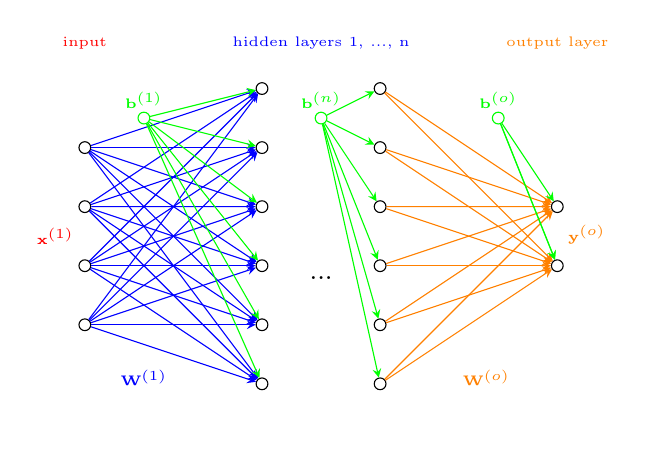
\begin{tikzpicture}[scale=1.5] 
\foreach \i in {0,...,3} \node[draw,circle,inner sep=1.5pt] (input\i) at (0,\the\numexpr0.5*\i+.5+0.75) {};
\foreach \i in {0,...,5} \node[draw,circle,inner sep=1.5pt] (hidden\i) at (1.5,\the\numexpr0.5*\i+0.75) {};
\foreach \i in {0,...,5} \node[draw,circle,inner sep=1.5pt] (hiddenl\i) at (2.5,\the\numexpr0.5*\i+0.75) {};
\foreach \i in {0,...,1} \node[draw,circle,inner sep=1.5pt] (output\i) at (4,\the\numexpr0.5*\i+1+.75) {};

% connectors input -> hidden
\foreach \i in {0,...,3}
\foreach \j in {0,...,5} \draw[-stealth,blue!100!white] (input\i) -- (hidden\j);

% connectors hidden -> output
\foreach \i in {0,...,5}
\foreach \j in {0,...,1} \draw[-stealth,orange!100!white] (hiddenl\i) -- (output\j);

% labels
\draw (input3) ++ (0.0,0.25+.5) node[red,above] {\tiny input};
\draw (output1) ++ (0.0,0.25+1.) node[orange,above] {\tiny output layer};
\draw (hidden5) ++ (0.5,0.25) node[blue,above] {\tiny hidden layers 1, ..., n};

%\draw (input0) ++ (-0.25,-0.20) node[red!100!white,above] {\tiny $x_1$};
\draw (input1) ++ (-0.25,.10) node[red!100!white,above] {\tiny $\mathbf{x}^{(1)}$};

%\draw (input1) ++ (-0.25,-0.20) node[red!100!white,above] {\tiny $x_0$};
%\draw (hiddenl5) ++ (0.0,0.25) node[blue,above] {\tiny hidden (n)};
\draw (output0) ++ (0.25,.10) node[orange,above] {\tiny $\mathbf{y}^{(o)}$};	
\draw (output0) ++ (0.25-2.25,-0.20) node[black,above] {...};	

% bias nodes
\node[color=green,draw,circle,inner sep=1.5pt] (bias1) at (0.5,5*0.5+0.5) {};
\draw (bias1) ++ (0.0,0.0) node[green,above] {\tiny $\textbf{b}^{\text{(1)}}$};

\node[color=green,draw,circle,inner sep=1.5pt] (bias3) at (0.5+1.5,5*0.5+0.5) {};
\draw (bias3) ++ (0.0,0.0) node[green,above] {\tiny $\textbf{b}^{\text{(n)}}$};

\node[color=green,draw,circle,inner sep=1.5pt] (bias2) at (2.25+1.25,5*0.5+0.5) {};
\draw (bias2) ++ (0.0,0.0) node[green,above] {\tiny $\textbf{b}^{\text{(o)}}$};

% bias connectors
\foreach \i in {0,...,5} \draw[-stealth,green!100!white] (bias1) -- (hidden\i);
\foreach \i in {0,...,5} \draw[-stealth,green!100!white] (bias3) -- (hiddenl\i);
\foreach \i in {0,...,1} \draw[-stealth,green!100!white] (bias2) -- (output\i);
\draw[-stealth,green!100!white] (bias2) -- (output0);

% weight labels
\draw (input0) ++ (0.5,-.6) node[blue!100!white,above] {\tiny $\textbf{W}^{\text{(1)}}$};
\draw (hiddenl0) ++ (.9,-0.1) node[orange!100!white,above] {\tiny $\textbf{W}^{\text{(o)}}$};

\node[draw,color=white] (dummy) at (0,0.5) {};
\end{tikzpicture}
	\caption[Deep artifical neural network]{Deep artifical neural network. An \acrfull{ann} can n hidden layers will always have an input $\mathbf{x}^{(1)})$ and one output layer $y^{(o)}$. The sizes of the input and the individual layers can vary depending on a chosen problem.} 
	\label{multilayernetwork}
\end{figure}
%\end{wrapfigure}
The supervised training of an \gls{ann} can be divided into a \emph{forward pass} where the output of all nodes is evaluated and a \emph{backward pass} which computes the respective parameter updates. In the \textbf{forward pass}, the input $\mathbf{x}^{(l)}$ of a layer $l$ sums to a net input $\mathbf{a}^{(l)}$ of
\begin{align*}
\mathbf{a}^{(l)} = W^{(l)} \, \mathbf{x}^{(l)} + \mathbf{b}^{(l)} + \left(\text{noise}\right), 
\end{align*}
with the weight matrix $W^{(l)}$, the bias $\mathbf{b}^{(l)}$ and an optional noise term. Depending on the task, the bias as well as the optional noise term can be vital: the individual biases for instance allow the network to adjust the dynamic range of each neuron and the injection of artificial noise can significantly increase the training performance (\citealp{an1996effects}).

The output $\mathbf{y}^{(l)}$ of the layer $l$ is then given by the activation function $\phi$, e.g. a sigmoid
\begin{equation*}
\mathbf{y}^{(l)} = \phi(\mathbf{a}^{(l)}) = \frac{1}{1 + e^{(-\beta \mathbf{a}^{(l)})}},
\end{equation*}
with the slope parameter $\beta$. Popular choices for the activation function besides a sigmoid are a \gls{relu} or the hyperbolic tangent ($\tanh$). In \cref{dltransfer} the various activation functions are shown for comparison. However, more important than the exact shape is that the chosen function is non-linear. A linear activation function makes any layer structure redundant, as the composition of linear linear functions yields again a linear function and therefore all layers of a deep network could be merged into a single one.

The same principle is then applied to all other layers to complete the forward pass, i.e. the result of the previous layer is the input for the current layer. The weight matrix $W^{\text{(l)}}$ connecting layer $l$ with $l-1$ has the appropriate shape to fit the number of input nodes $n^{\text{(l-1)}}_\text{nodes}$ and output nodes $n^{\text{(l)}}_\text{nodes}$.

\begin{figure}
	\begin{subfigure}[c]{0.5\textwidth}
		\centering
		\caption{}
		\inputpgf{figures}{deeplearning_activation_functions.pgf}
		\label{dltransfer}
	\end{subfigure}
	\begin{subfigure}[c]{0.5\textwidth}
		\centering
		\caption{}
		\inputpgf{figures}{deeplearning_activation_functions_derivative.pgf}	
		\label{dltransfergradient}
	\end{subfigure}
	\caption[Popular shapes for activation functions in deep learning.]{Popular shapes for activation functions in deep learning. \textbf{(\subref{dltransfer})}: Some of the most popular shapes for the activation function are a \gls{relu}, $\tanh$ or sigmoid. \textbf{(\subref{dltransfergradient})}: The derivative of the different activation function gives an insight how the impact of gradient descent changes for different functions. In the case of the sigmoid and the hyperbolic tangent, either a very high or low input leads to a zero gradient and thus to a vanishing parameter update.}
	\label{deeplearning_activation_functions}
\end{figure}

In deep learning, \emph{gradient descent} is probably the most popular algorithm to perform the \textbf{backward pass} on a network. A differentiable loss function $\loss(\mathbf{\mathbf{x}, y^*, \theta})$ for a given target $\textbf{y}^*$ is minimized. Here, a binary cross-entropy loss is chosen
\begin{equation*}
\mathcal{L} = - \frac{1}{N} \sum_{i=1}^N \textbf{y}^* \log(\textbf{y}_i + (1-\textbf{y}^*) \log(1 - \textbf{y}_i), 
\end{equation*}
with a minibatch of size $N$ and the target $\textbf{y}^*$ being scaled between 0 and 1. In combination with a sigmoid-shaped activation function, this choice becomes convenient when computing the new set of parameters $\mathbf{\theta}'$. This is done by moving along the negative gradient of the loss with respect to the network's parameters $\mathbf{\theta}$
\begin{equation}
\mathbf{\theta'} = \mathbf{\theta} - \eta \, \nabla_\theta\loss(\mathbf{\mathbf{x}, y^*, \mathbf{\theta}}),
\label{stochasticgradientdescent}
\end{equation}
with the learning rate $\eta$. To avoid extensive computational costs, the gradient is estimated by a uniformly drawn subset of the full training data set, a \emph{minibatch}. In particular, if the size of the minibatch equals one, one speaks of \gls{sgd}. As an example, the updates of the weight matrices of a single hidden layer network are computed in the next paragraphs using \gls{sgd}.

First, the derivative of the cross entropy loss function in the output layer $l\equiv o$ is computed
\begin{equation*}
\frac{\partial\mathcal{L}}{\partial \mathbf{y}^{(o)}} = 
- \frac{\mathbf{y}^*}{\mathbf{y}^{(o)}} + 
\frac{1 - \mathbf{y}^*}{1 - \mathbf{y}^{(o)}},
\end{equation*}
The gradient of the loss can then be rewritten in terms of the error $\mathbf{e}^{(o)} = \mathbf{y}^* - \mathbf{y}^{(o)}$ by using the derivative of the activation function
\begin{align*}
\frac{\partial \mathbf{y}^{(o)}}{\partial \mathbf{a}^{(o)}} = \frac{\partial \gls{activation}(\mathbf{a}^{(o)})}{\partial \mathbf{a}^{(o)}} = \gls{activation} (1 - \gls{activation}),\\
\Rightarrow \quad \frac{\partial\mathcal{L}}{\partial \mathbf{a}^{(o)}} =
\frac{\partial\mathcal{L}}{\partial \mathbf{y}^{(o)}} 
\; \frac{\partial \mathbf{y}^{(o)}}{\partial \mathbf{a}^{(o)}} =
\mathbf{y}^* - \mathbf{y}^{(o)} = \mathbf{e}^{(o)}.
\end{align*}

According to \cref{stochasticgradientdescent}, the final update of the weight matrix is given by
\begin{equation}
\delta W^{(o)} = - \eta \frac{\partial \mathcal{L}}{\partial W^{(o)}} 
= - \eta \;
\frac{\partial\mathcal{L}}{\partial \mathbf{y}^{(o)}} \;
\frac{\partial \mathbf{a}^{(o)}}{\partial W^{(o)}}
= - \eta \, \left(\mathbf{e}^{(o)} \mathbf{x}^{(o),T}\right),
\label{backpropupdate}
\end{equation}
with the transpose of the input $x^{(o),T}$.

The computation for the hidden layer ($l\equiv h$) can be done in a similar fashion. Again, the gradient of the loss function is computed
\begin{equation*}
\frac{\partial\mathcal{L}}{\partial \mathbf{a}^{(h)}} = \mathbf{e}^{(h)} \;
\frac{\partial \mathbf{y}^{(h)} }{\partial \mathbf{a}^{(h)}}.
\end{equation*}
The error of the output layer $\mathbf{e}^{(o)}$ is propagated backwards with the transpose of the weight matrix $W^{(o),T}$ as $\mathbf{e}^{(h)}=W^{(o),T}\mathbf{e}^{(o)}$ yielding a total update of
\begin{equation*}
\delta W^{\text{(h)}} = - \eta \;
\left(W^{\text{(o)}T} \mathbf{e}^{(o)}\right) \;
\frac{\partial \mathbf{y}^{(h)} }{\partial \mathbf{a}^{(h)}} \; \mathbf{x}^{(h), T}.
\end{equation*}

The backward propagation of the error is eponymous for the method's name \textit{backpropagation}. Despite the great performance for many deep learning tasks, the biological plausibility of propagating the error signal backward has been questioned ever since (\citealp{grossberg1987competitive}). A simple but effective adjustment was suggested by \cite{lillicrap2016random} which is also known as \textit{feedback alignment}. Instead of the transpose of the feedforward weight matrix, a fixed random matrix $B$ is chosen to propagate the error backwards. Compared to the backpropagation variant from \cref{backpropupdate} the update in the hidden layer changes to
\begin{equation*}
\delta W^{(h)} = - \eta \;
(B \mathbf{e}^{(o)}) \;
\frac{\partial \mathbf{y}^{(h)}}{\partial \mathbf{a}^{(h)}} \;
\mathbf{x}^{(h),T}.
\end{equation*}
The only constraint to $B$ is that $\mathbf{e}^{(o)T} W^{(o)} B \mathbf{e}^{(o)} > 0$ has to be fulfilled on average, meaning that geometrically, the new feedback signal $B \mathbf{e}^{(o)}$ for the hidden layer lies within $90^{\circ}$ of the one used by backpropagation, $W^{\text{(o)}T} \mathbf{e}^{(o)}$.

%Q:Überleitung zu biologischem neuron hier?

\section{The Biological Neuron}

Biological neural networks have been a great inspiration for deep learning algorithms and \glspl{ann}. It is estimated that the human brain contains around $10^{11}$ neurons of different shape, size and functions (\citealp{numberofneurons}). By the use of \emph{synapses}, \emph{presynaptic} neurons connect to \emph{postsynaptic} ones and thereby create complex network structures throughout the brain. A postsynaptic neuron has usually around $10^4$ presynaptic partners (\citealp{numberofsynapses}). The connections vary from dense clusters with nearby neurons to linking distant brain regions with each other. 

Most neurons can be divided into three functional parts: \emph{dendrites}, \emph{soma} and \emph{axon} (c.f. \cref{biologicalneuron}). At the dendrites a postsynaptic neuron receives inputs from its presynaptic partners. These inputs are converted into \glspl{psp} using charged molecules corresponding to a variable graded potential in size and shape. The \glspl{psp} are then relayed to the soma where they are integrated over. Depending on the nature of synaptic connection, the stimulation has either an excitatory or inhibitory effect on the neuron, resulting in an increased or decreased membrane potential. Over time the unbalanced ion concentration in and outside the membrane is restored by the membranes permeability and additional ion pumps. In an equilibrated state the membrane potential is referred to as the \emph{resting potential}. (\citealp{gerstner2014dynamics})

Given a continuous excitatory stimulation current, the neuron will trigger a fire mechanism once a certain threshold potential is reached. The neuron's membrane becomes hyperpolarized and decreases even below the resting potential as shown in \cref{actionpotential} entering a \emph{refractory period}. During this period it remains hard but not impossible for the neuron to fire again due to the ongoing hyperpolarization of the membrane. This mechanism releases an electrochemical pulse a so-called action potential or spike, which is then relayed by the axon to the connected partners at the end of the axon. (\citealp{gerstner2014dynamics})

\begin{figure}
	\begin{subfigure}{0.5\textwidth}
		\centering
		\caption{}
		\vspace{0.75cm}
		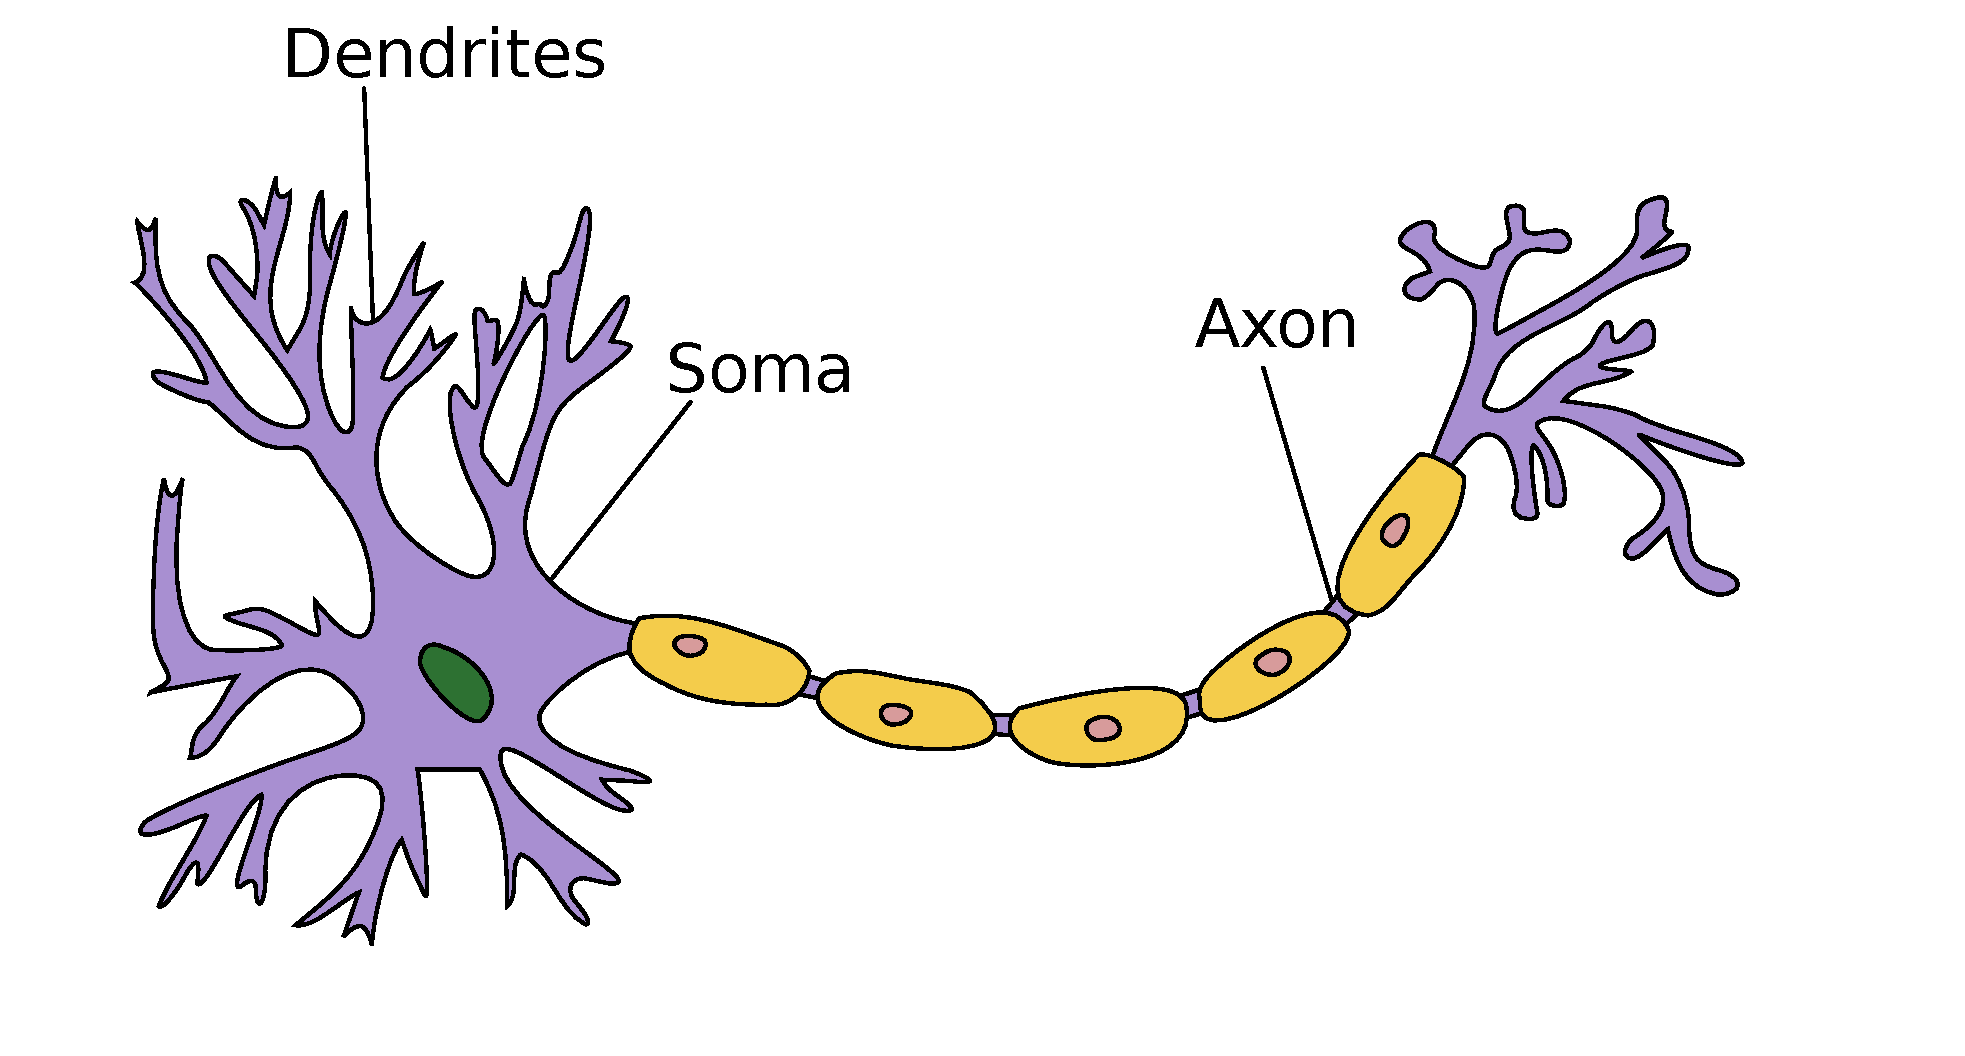
\includegraphics[width=\linewidth, valign=t]{figures/Neuron.pdf}
		\vspace{1.25cm}	
		\label{biosynapse}
	\end{subfigure}
	\begin{subfigure}{0.5\textwidth}
		\centering
		\caption{}
		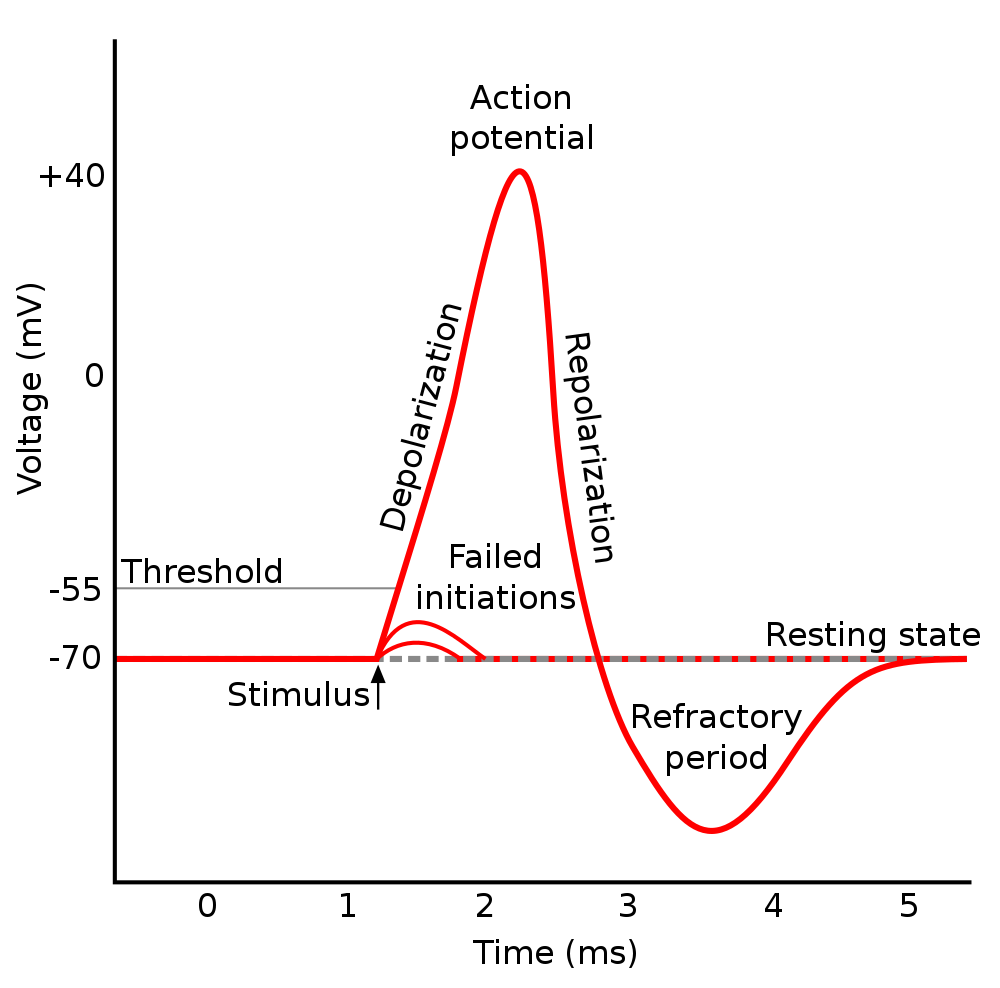
\includegraphics[width=0.8\linewidth, valign=t]{figures/action_potential.png}
		\label{actionpotential}
	\end{subfigure}
	\caption[Schematics of a biological neuron and an action potential]{Schematics of a biological neuron and an action potential. \textbf{(\subref{biosynapse})} A biological neuron can be split into three main functional parts. The dendrites collect the inputs from presynaptic partners and relay them in the form of \glsreset{psp}\glspl{psp} to the soma. The soma integrates the \glspl{psp} and eventually triggers a fire response. The axon relays this response to the connected neurons at the end of the axon. Figure adapted from \citealp{picture_neuron}. \textbf{(\subref{actionpotential})} The fire response of neuron after exceeding the threshold is called action potential or spike. After a phase of depolarization, the membrane repolarizes and enters the refractory periode during which it is hard but not impossible to fire again. Figure taken from \citealp{picture_actionpotential}.}
	\label{biologicalneuron}
	
\end{figure}

The action potential releases various neurotransmitter to overcome a small but physical gap at the synapses, the synaptic cleft. Once a transmitter has docked to a corresponding receptor on the other side, activated ion channels convert the chemical transmission back into an electrical signal resembling the \gls{psp}. Depending on the type of neuro\-transmitters the excitation can be excitatory or inhibitory (\citealp{gerstner2014dynamics}). According to Dale's principle a presynaptic neuron releases always the same type of neurotransmitter (\citealp{dale1935pharmacology}). To that end, a neuron's output is either excitatory or inhibitory but not both. The input of a neuron, on the other side, is not restricted to a single type of excitation, as various presynaptic partners can be connected. 

A wide-spread assumption in the field of neuroscience is that the exact shape of a spike doesn't carry any relevant information and therefore all spikes can be modeled by a stereotypical shape. However, recent research has already suggested that the small variations in the action potential contain vital information (\citealp{debanne2013mechanisms}). For the prior assumption, the communication between neurons is reduced to a temporal and spatial dimension. Temporal information is encoded either in the frequency (\emph{rate coding}) or the precise timing (\emph{time coding}) of spikes whereas the spatial dimension is filled with varying populations of neurons (\citealp{gerstner2014dynamics}). A more detailed description of neural coding schemes is presented in section \ref{neuralcoding}.

The brain has an ability to continuously change the topology of its synaptic wiring, to create new synapses, to alter the chemical properties of the synaptic receptors or to simply strengthen and weaken the synaptic efficacy. With these \emph{plasticity} mechanisms the brain is able to learn and adapt as a reaction to stimulation or even damage. (\citealp{gerstner2014dynamics})

One way of learning and forming memory is known as synaptic plasticity where the synaptic strength is changed over time. According to Hebb's theory ``neurons that fire together wire together" (\citealp{hebb1949organization}). An experimental proof of such activity-dependent plasticity was found by \citealp{bliss1973long}, where they discovered that a short but high frequency stimulation lead to a long lasting change in the synapse's efficacy. This is also referred to as \gls{ltp}. Reducing the stimulus to a low frequency, on the other hand, resulted in the opposite effect: \gls{ltd}. In combination they can carve out certain regions in the brain which is related to a specific stimulus and thereby create memory (\citealp{nabavi2014engineering}). A better understanding of \gls{ltp} and \gls{ltd} was gained when \gls{stdp} was first observed (\citealp{markram1997regulation}, \citealp{poo98stdp}). \gls{stdp} shows in principle that presynaptic activity just before a postsynaptic response leads to an increased synaptic strength. If presynaptic activity occurs right after a postsynaptic spike, the synapses is weakened. 

Such plasticity mechanism are self-regulating and independent of any reward-giving structure. In analogy to the learning concepts introduced by deep learning, they are also referred to as unsupervised Hebbian learning. However, these methods fall short of successfully training the brain to master complex action-required tasks, as the outcome of a decision made by the brain is not part of the plasticity mechanism. Hence, a behavioral learning strategy requires knowledge over the outcome of taken decisions and needs to remember which decisions have lead to rewards, as the reward in real life is often delayed. (\citealp{gerstner2014dynamics})

Developing biologically inspired and plausible supervised learning algorithms is a dedicated goal in the field of modern neuroscience. Before discussing two such candidates in more detail, a practicable model of the biological neuron is presented first. This model is implemented in the analog core of the neuromorphic platform \gls{bss2} and resembles the basis of all experimental work presented in this thesis.

\section{The \acrlong{lif} Model}
\label{lifmodel}

An early but successful description of the biological neuron dynamics was accomplished by the \glsfirst{lif} neuron model, first described by \cite{lapicque1907recherches}. Despite some strong simplifications, the main dynamics of the membrane potential are well described by the model and it thus has been a popular and portable choice for neuromorphic hardware implementations.

In biology, the observation of similar shaped individual action potentials lead to the assumption that the shape of a spike does not transport any information. The \gls{lif} model is based upon this theory and thus every spike can be replaced by a stereotypical shape (\citealp{gerstner2014dynamics}). 

Another observation in biology is that neurons vary much in their shape and size fulfilling different functions. The spatial component plays an important role for the dynamics of a neuron. For instance, the strategic positioning of certain excitatory or inhibitory inputs on the dendrites, either closer or farther away from the soma, give rise to non-linear behavior in the course of the membrane potential. However, extensive spatial dependencies are difficult and costly to implement in a model. Therefore, the \gls{lif} neuron neglects the topology of the neuron and is approximated as a point-like integrator. (\citealp{gerstner2014dynamics})

In the model, the incoming spike train $S_j(t)$ from various presynaptic partners $j$ is described by a series of spikes $s$ at times $t_j^{(s)}$
\begin{equation*}
S_j(t) = \sum_s \delta(t - t_j^{(s)}),
\end{equation*}
with the $\delta$-function denoted as $\delta$. 

Each spike of the input spike train evokes a \gls{psp}. The impact of the \glspl{psp} depends on the individual synaptic weights $w_j$. For simplicity, the excitatory or inhibitory nature of the synapses is encoded by a sign in the synaptic weight as well. Summing over all input sources yields a total synaptic input current that is seen by the postsynaptic neuron
\begin{equation}
\gls{isyn}(t) = \sum_j w_j \left(\epsilon \ast S_j(t)\right),
\label{synaptic_input}
\end{equation}
with the convolution of a double exponential kernel $\epsilon$ with the input spike train $\epsilon \ast S_j$ describing the shape of a single \gls{psp}. The kernel can be defined as
\begin{align*}
\epsilon_\text{double}(t) 	&=\frac{1}{\mathcal{N}} \left(\epsilon_\text{rise} \ast \epsilon_\text{fall}\right)(t) \\
&=\frac{1}{\mathcal{N}}\exp \left(-\frac{t}{\tau_\text{rise}} \right)  \ast \exp \left(-\frac{t}{\tau_\text{fall}} \right), 
%\label{exponentialkernels)}
\end{align*}
with a rising and falling time constant $\tau_\text{rise}$ and $\tau_\text{fall}$ respectively. A constant $\mathcal{N}$ norms the kernel to unity. As the rising constant goes to zero $\tau_\text{rise} \rightarrow 0$ the double exponential turns into a single exponential kernel $\epsilon_\text{single} = \epsilon_\text{fall}$.

The membrane potential \gls{v_mem} changes with the continuous synaptic input causing an unbalanced ion concentration inside the membrane. Passive as well as active processes are permanently restoring the membrane potential back to its equilibrium state which is associated with the resting potential \gls{v_leak}. In the \gls{lif} model, the temporal scale of these restoring processes is defined by the membranes capacitance $C_\text{m}$ and the leakage conductance $g_\text{leak}$ yielding the membrane's time constant $\gls{tau_m} = \frac{C_\text{m}}{g_\text{leak}}$. The dynamics of the membrane are then given by a single differential equation
\begin{align}
\label{lifeq}
C_{\text{m}} \frac{d\gls{v_mem}}{dt} &= -g_{\text{leak}} (\gls{v_mem} - \gls{v_leak}) + \gls{isyn}.
\end{align}

As for a biological neuron, a \gls{lif} neuron triggers a spike once a certain threshold \gls{thres} is crossed following the condition
\begin{equation*}
\gls{v_mem}\big(t^{(s)}\big) = \gls{thres} \Leftrightarrow \text{neuron fires at time } t^{(s)}.
\end{equation*}

Then the membrane is set to a reset potential \gls{v_reset} where it remains unchanged for a refractory period of \gls{refrac}
\begin{equation*}
\gls{v_mem}(t) = \gls{v_reset} \quad \forall t \in \left(t^{(s)}, t^{(s)} + \gls{refrac}\right].
\end{equation*}
Unlike for its biological counterpart, the modeled neuron cannot spike during the refractory period.

\begin{figure}
	\centering
	\scalebox{0.93}{%% Creator: Matplotlib, PGF backend
%%
%% To include the figure in your LaTeX document, write
%%   \input{<filename>.pgf}
%%
%% Make sure the required packages are loaded in your preamble
%%   \usepackage{pgf}
%%
%% Figures using additional raster images can only be included by \input if
%% they are in the same directory as the main LaTeX file. For loading figures
%% from other directories you can use the `import` package
%%   \usepackage{import}
%% and then include the figures with
%%   \import{<path to file>}{<filename>.pgf}
%%
%% Matplotlib used the following preamble
%%   \usepackage[utf8]{inputenc}
%%   \usepackage[T1]{fontenc}
%%   \usepackage{textcomp}
%%
\begingroup%
\makeatletter%
\begin{pgfpicture}%
\pgfpathrectangle{\pgfpointorigin}{\pgfqpoint{4.902605in}{2.799288in}}%
\pgfusepath{use as bounding box, clip}%
\begin{pgfscope}%
\pgfsetbuttcap%
\pgfsetmiterjoin%
\pgfsetlinewidth{0.000000pt}%
\definecolor{currentstroke}{rgb}{0.000000,0.000000,0.000000}%
\pgfsetstrokecolor{currentstroke}%
\pgfsetstrokeopacity{0.000000}%
\pgfsetdash{}{0pt}%
\pgfpathmoveto{\pgfqpoint{0.000000in}{0.000000in}}%
\pgfpathlineto{\pgfqpoint{4.902605in}{0.000000in}}%
\pgfpathlineto{\pgfqpoint{4.902605in}{2.799288in}}%
\pgfpathlineto{\pgfqpoint{0.000000in}{2.799288in}}%
\pgfpathclose%
\pgfusepath{}%
\end{pgfscope}%
\begin{pgfscope}%
\pgfsetbuttcap%
\pgfsetmiterjoin%
\pgfsetlinewidth{0.000000pt}%
\definecolor{currentstroke}{rgb}{0.000000,0.000000,0.000000}%
\pgfsetstrokecolor{currentstroke}%
\pgfsetstrokeopacity{0.000000}%
\pgfsetdash{}{0pt}%
\pgfpathmoveto{\pgfqpoint{0.585105in}{2.064876in}}%
\pgfpathlineto{\pgfqpoint{4.847605in}{2.064876in}}%
\pgfpathlineto{\pgfqpoint{4.847605in}{2.744288in}}%
\pgfpathlineto{\pgfqpoint{0.585105in}{2.744288in}}%
\pgfpathclose%
\pgfusepath{}%
\end{pgfscope}%
\begin{pgfscope}%
\pgfsetbuttcap%
\pgfsetroundjoin%
\definecolor{currentfill}{rgb}{0.200000,0.200000,0.200000}%
\pgfsetfillcolor{currentfill}%
\pgfsetlinewidth{0.803000pt}%
\definecolor{currentstroke}{rgb}{0.200000,0.200000,0.200000}%
\pgfsetstrokecolor{currentstroke}%
\pgfsetdash{}{0pt}%
\pgfsys@defobject{currentmarker}{\pgfqpoint{0.000000in}{-0.048611in}}{\pgfqpoint{0.000000in}{0.000000in}}{%
\pgfpathmoveto{\pgfqpoint{0.000000in}{0.000000in}}%
\pgfpathlineto{\pgfqpoint{0.000000in}{-0.048611in}}%
\pgfusepath{stroke,fill}%
}%
\begin{pgfscope}%
\pgfsys@transformshift{0.585105in}{2.064876in}%
\pgfsys@useobject{currentmarker}{}%
\end{pgfscope}%
\end{pgfscope}%
\begin{pgfscope}%
\pgfsetbuttcap%
\pgfsetroundjoin%
\definecolor{currentfill}{rgb}{0.200000,0.200000,0.200000}%
\pgfsetfillcolor{currentfill}%
\pgfsetlinewidth{0.803000pt}%
\definecolor{currentstroke}{rgb}{0.200000,0.200000,0.200000}%
\pgfsetstrokecolor{currentstroke}%
\pgfsetdash{}{0pt}%
\pgfsys@defobject{currentmarker}{\pgfqpoint{0.000000in}{-0.048611in}}{\pgfqpoint{0.000000in}{0.000000in}}{%
\pgfpathmoveto{\pgfqpoint{0.000000in}{0.000000in}}%
\pgfpathlineto{\pgfqpoint{0.000000in}{-0.048611in}}%
\pgfusepath{stroke,fill}%
}%
\begin{pgfscope}%
\pgfsys@transformshift{1.153438in}{2.064876in}%
\pgfsys@useobject{currentmarker}{}%
\end{pgfscope}%
\end{pgfscope}%
\begin{pgfscope}%
\pgfsetbuttcap%
\pgfsetroundjoin%
\definecolor{currentfill}{rgb}{0.200000,0.200000,0.200000}%
\pgfsetfillcolor{currentfill}%
\pgfsetlinewidth{0.803000pt}%
\definecolor{currentstroke}{rgb}{0.200000,0.200000,0.200000}%
\pgfsetstrokecolor{currentstroke}%
\pgfsetdash{}{0pt}%
\pgfsys@defobject{currentmarker}{\pgfqpoint{0.000000in}{-0.048611in}}{\pgfqpoint{0.000000in}{0.000000in}}{%
\pgfpathmoveto{\pgfqpoint{0.000000in}{0.000000in}}%
\pgfpathlineto{\pgfqpoint{0.000000in}{-0.048611in}}%
\pgfusepath{stroke,fill}%
}%
\begin{pgfscope}%
\pgfsys@transformshift{1.721772in}{2.064876in}%
\pgfsys@useobject{currentmarker}{}%
\end{pgfscope}%
\end{pgfscope}%
\begin{pgfscope}%
\pgfsetbuttcap%
\pgfsetroundjoin%
\definecolor{currentfill}{rgb}{0.200000,0.200000,0.200000}%
\pgfsetfillcolor{currentfill}%
\pgfsetlinewidth{0.803000pt}%
\definecolor{currentstroke}{rgb}{0.200000,0.200000,0.200000}%
\pgfsetstrokecolor{currentstroke}%
\pgfsetdash{}{0pt}%
\pgfsys@defobject{currentmarker}{\pgfqpoint{0.000000in}{-0.048611in}}{\pgfqpoint{0.000000in}{0.000000in}}{%
\pgfpathmoveto{\pgfqpoint{0.000000in}{0.000000in}}%
\pgfpathlineto{\pgfqpoint{0.000000in}{-0.048611in}}%
\pgfusepath{stroke,fill}%
}%
\begin{pgfscope}%
\pgfsys@transformshift{2.290105in}{2.064876in}%
\pgfsys@useobject{currentmarker}{}%
\end{pgfscope}%
\end{pgfscope}%
\begin{pgfscope}%
\pgfsetbuttcap%
\pgfsetroundjoin%
\definecolor{currentfill}{rgb}{0.200000,0.200000,0.200000}%
\pgfsetfillcolor{currentfill}%
\pgfsetlinewidth{0.803000pt}%
\definecolor{currentstroke}{rgb}{0.200000,0.200000,0.200000}%
\pgfsetstrokecolor{currentstroke}%
\pgfsetdash{}{0pt}%
\pgfsys@defobject{currentmarker}{\pgfqpoint{0.000000in}{-0.048611in}}{\pgfqpoint{0.000000in}{0.000000in}}{%
\pgfpathmoveto{\pgfqpoint{0.000000in}{0.000000in}}%
\pgfpathlineto{\pgfqpoint{0.000000in}{-0.048611in}}%
\pgfusepath{stroke,fill}%
}%
\begin{pgfscope}%
\pgfsys@transformshift{2.858438in}{2.064876in}%
\pgfsys@useobject{currentmarker}{}%
\end{pgfscope}%
\end{pgfscope}%
\begin{pgfscope}%
\pgfsetbuttcap%
\pgfsetroundjoin%
\definecolor{currentfill}{rgb}{0.200000,0.200000,0.200000}%
\pgfsetfillcolor{currentfill}%
\pgfsetlinewidth{0.803000pt}%
\definecolor{currentstroke}{rgb}{0.200000,0.200000,0.200000}%
\pgfsetstrokecolor{currentstroke}%
\pgfsetdash{}{0pt}%
\pgfsys@defobject{currentmarker}{\pgfqpoint{0.000000in}{-0.048611in}}{\pgfqpoint{0.000000in}{0.000000in}}{%
\pgfpathmoveto{\pgfqpoint{0.000000in}{0.000000in}}%
\pgfpathlineto{\pgfqpoint{0.000000in}{-0.048611in}}%
\pgfusepath{stroke,fill}%
}%
\begin{pgfscope}%
\pgfsys@transformshift{3.426772in}{2.064876in}%
\pgfsys@useobject{currentmarker}{}%
\end{pgfscope}%
\end{pgfscope}%
\begin{pgfscope}%
\pgfsetbuttcap%
\pgfsetroundjoin%
\definecolor{currentfill}{rgb}{0.200000,0.200000,0.200000}%
\pgfsetfillcolor{currentfill}%
\pgfsetlinewidth{0.803000pt}%
\definecolor{currentstroke}{rgb}{0.200000,0.200000,0.200000}%
\pgfsetstrokecolor{currentstroke}%
\pgfsetdash{}{0pt}%
\pgfsys@defobject{currentmarker}{\pgfqpoint{0.000000in}{-0.048611in}}{\pgfqpoint{0.000000in}{0.000000in}}{%
\pgfpathmoveto{\pgfqpoint{0.000000in}{0.000000in}}%
\pgfpathlineto{\pgfqpoint{0.000000in}{-0.048611in}}%
\pgfusepath{stroke,fill}%
}%
\begin{pgfscope}%
\pgfsys@transformshift{3.995105in}{2.064876in}%
\pgfsys@useobject{currentmarker}{}%
\end{pgfscope}%
\end{pgfscope}%
\begin{pgfscope}%
\pgfsetbuttcap%
\pgfsetroundjoin%
\definecolor{currentfill}{rgb}{0.200000,0.200000,0.200000}%
\pgfsetfillcolor{currentfill}%
\pgfsetlinewidth{0.803000pt}%
\definecolor{currentstroke}{rgb}{0.200000,0.200000,0.200000}%
\pgfsetstrokecolor{currentstroke}%
\pgfsetdash{}{0pt}%
\pgfsys@defobject{currentmarker}{\pgfqpoint{0.000000in}{-0.048611in}}{\pgfqpoint{0.000000in}{0.000000in}}{%
\pgfpathmoveto{\pgfqpoint{0.000000in}{0.000000in}}%
\pgfpathlineto{\pgfqpoint{0.000000in}{-0.048611in}}%
\pgfusepath{stroke,fill}%
}%
\begin{pgfscope}%
\pgfsys@transformshift{4.563438in}{2.064876in}%
\pgfsys@useobject{currentmarker}{}%
\end{pgfscope}%
\end{pgfscope}%
\begin{pgfscope}%
\pgfpathrectangle{\pgfqpoint{0.585105in}{2.064876in}}{\pgfqpoint{4.262500in}{0.679412in}} %
\pgfusepath{clip}%
\pgfsetrectcap%
\pgfsetroundjoin%
\pgfsetlinewidth{0.803000pt}%
\definecolor{currentstroke}{rgb}{0.690196,0.690196,0.690196}%
\pgfsetstrokecolor{currentstroke}%
\pgfsetstrokeopacity{0.300000}%
\pgfsetdash{}{0pt}%
\pgfpathmoveto{\pgfqpoint{0.585105in}{2.214661in}}%
\pgfpathlineto{\pgfqpoint{4.847605in}{2.214661in}}%
\pgfusepath{stroke}%
\end{pgfscope}%
\begin{pgfscope}%
\pgfsetbuttcap%
\pgfsetroundjoin%
\definecolor{currentfill}{rgb}{0.200000,0.200000,0.200000}%
\pgfsetfillcolor{currentfill}%
\pgfsetlinewidth{0.803000pt}%
\definecolor{currentstroke}{rgb}{0.200000,0.200000,0.200000}%
\pgfsetstrokecolor{currentstroke}%
\pgfsetdash{}{0pt}%
\pgfsys@defobject{currentmarker}{\pgfqpoint{-0.048611in}{0.000000in}}{\pgfqpoint{0.000000in}{0.000000in}}{%
\pgfpathmoveto{\pgfqpoint{0.000000in}{0.000000in}}%
\pgfpathlineto{\pgfqpoint{-0.048611in}{0.000000in}}%
\pgfusepath{stroke,fill}%
}%
\begin{pgfscope}%
\pgfsys@transformshift{0.585105in}{2.214661in}%
\pgfsys@useobject{currentmarker}{}%
\end{pgfscope}%
\end{pgfscope}%
\begin{pgfscope}%
\definecolor{textcolor}{rgb}{0.200000,0.200000,0.200000}%
\pgfsetstrokecolor{textcolor}%
\pgfsetfillcolor{textcolor}%
\pgftext[x=0.240968in,y=2.166833in,left,base]{\color{textcolor}\rmfamily\fontsize{10.000000}{12.000000}\selectfont \(\displaystyle -60\)}%
\end{pgfscope}%
\begin{pgfscope}%
\pgfpathrectangle{\pgfqpoint{0.585105in}{2.064876in}}{\pgfqpoint{4.262500in}{0.679412in}} %
\pgfusepath{clip}%
\pgfsetrectcap%
\pgfsetroundjoin%
\pgfsetlinewidth{0.803000pt}%
\definecolor{currentstroke}{rgb}{0.690196,0.690196,0.690196}%
\pgfsetstrokecolor{currentstroke}%
\pgfsetstrokeopacity{0.300000}%
\pgfsetdash{}{0pt}%
\pgfpathmoveto{\pgfqpoint{0.585105in}{2.690272in}}%
\pgfpathlineto{\pgfqpoint{4.847605in}{2.690272in}}%
\pgfusepath{stroke}%
\end{pgfscope}%
\begin{pgfscope}%
\pgfsetbuttcap%
\pgfsetroundjoin%
\definecolor{currentfill}{rgb}{0.200000,0.200000,0.200000}%
\pgfsetfillcolor{currentfill}%
\pgfsetlinewidth{0.803000pt}%
\definecolor{currentstroke}{rgb}{0.200000,0.200000,0.200000}%
\pgfsetstrokecolor{currentstroke}%
\pgfsetdash{}{0pt}%
\pgfsys@defobject{currentmarker}{\pgfqpoint{-0.048611in}{0.000000in}}{\pgfqpoint{0.000000in}{0.000000in}}{%
\pgfpathmoveto{\pgfqpoint{0.000000in}{0.000000in}}%
\pgfpathlineto{\pgfqpoint{-0.048611in}{0.000000in}}%
\pgfusepath{stroke,fill}%
}%
\begin{pgfscope}%
\pgfsys@transformshift{0.585105in}{2.690272in}%
\pgfsys@useobject{currentmarker}{}%
\end{pgfscope}%
\end{pgfscope}%
\begin{pgfscope}%
\definecolor{textcolor}{rgb}{0.200000,0.200000,0.200000}%
\pgfsetstrokecolor{textcolor}%
\pgfsetfillcolor{textcolor}%
\pgftext[x=0.240968in,y=2.642444in,left,base]{\color{textcolor}\rmfamily\fontsize{10.000000}{12.000000}\selectfont \(\displaystyle -40\)}%
\end{pgfscope}%
\begin{pgfscope}%
\pgftext[x=0.185413in,y=2.404582in,,bottom,rotate=90.000000]{\rmfamily\fontsize{10.000000}{12.000000}\selectfont \(\displaystyle V^\mathrm{LIF}_\mathrm{m}\) [mV]}%
\end{pgfscope}%
\begin{pgfscope}%
\pgfpathrectangle{\pgfqpoint{0.585105in}{2.064876in}}{\pgfqpoint{4.262500in}{0.679412in}} %
\pgfusepath{clip}%
\pgfsetrectcap%
\pgfsetroundjoin%
\pgfsetlinewidth{0.501875pt}%
\definecolor{currentstroke}{rgb}{0.400000,0.400000,0.400000}%
\pgfsetstrokecolor{currentstroke}%
\pgfsetdash{}{0pt}%
\pgfpathmoveto{\pgfqpoint{0.585105in}{2.214661in}}%
\pgfpathlineto{\pgfqpoint{1.153438in}{2.214661in}}%
\pgfpathlineto{\pgfqpoint{1.165373in}{2.248444in}}%
\pgfpathlineto{\pgfqpoint{1.177308in}{2.275828in}}%
\pgfpathlineto{\pgfqpoint{1.189812in}{2.298970in}}%
\pgfpathlineto{\pgfqpoint{1.202315in}{2.317542in}}%
\pgfpathlineto{\pgfqpoint{1.215387in}{2.333049in}}%
\pgfpathlineto{\pgfqpoint{1.229027in}{2.345844in}}%
\pgfpathlineto{\pgfqpoint{1.243803in}{2.356644in}}%
\pgfpathlineto{\pgfqpoint{1.259717in}{2.365526in}}%
\pgfpathlineto{\pgfqpoint{1.277903in}{2.373054in}}%
\pgfpathlineto{\pgfqpoint{1.298932in}{2.379227in}}%
\pgfpathlineto{\pgfqpoint{1.323938in}{2.384135in}}%
\pgfpathlineto{\pgfqpoint{1.355197in}{2.387892in}}%
\pgfpathlineto{\pgfqpoint{1.397253in}{2.390571in}}%
\pgfpathlineto{\pgfqpoint{1.462043in}{2.392233in}}%
\pgfpathlineto{\pgfqpoint{1.594465in}{2.392939in}}%
\pgfpathlineto{\pgfqpoint{1.727455in}{2.393008in}}%
\pgfpathlineto{\pgfqpoint{1.739390in}{2.359226in}}%
\pgfpathlineto{\pgfqpoint{1.751325in}{2.331843in}}%
\pgfpathlineto{\pgfqpoint{1.763828in}{2.308702in}}%
\pgfpathlineto{\pgfqpoint{1.776332in}{2.290131in}}%
\pgfpathlineto{\pgfqpoint{1.789403in}{2.274624in}}%
\pgfpathlineto{\pgfqpoint{1.803043in}{2.261830in}}%
\pgfpathlineto{\pgfqpoint{1.817820in}{2.251031in}}%
\pgfpathlineto{\pgfqpoint{1.833733in}{2.242149in}}%
\pgfpathlineto{\pgfqpoint{1.851920in}{2.234621in}}%
\pgfpathlineto{\pgfqpoint{1.872948in}{2.228448in}}%
\pgfpathlineto{\pgfqpoint{1.897955in}{2.223540in}}%
\pgfpathlineto{\pgfqpoint{1.929213in}{2.219784in}}%
\pgfpathlineto{\pgfqpoint{1.971270in}{2.217105in}}%
\pgfpathlineto{\pgfqpoint{2.036060in}{2.215443in}}%
\pgfpathlineto{\pgfqpoint{2.168482in}{2.214737in}}%
\pgfpathlineto{\pgfqpoint{2.869805in}{2.214661in}}%
\pgfpathlineto{\pgfqpoint{2.881740in}{2.263309in}}%
\pgfpathlineto{\pgfqpoint{2.893675in}{2.302742in}}%
\pgfpathlineto{\pgfqpoint{2.905610in}{2.334705in}}%
\pgfpathlineto{\pgfqpoint{2.917545in}{2.360615in}}%
\pgfpathlineto{\pgfqpoint{2.930048in}{2.382511in}}%
\pgfpathlineto{\pgfqpoint{2.942552in}{2.400083in}}%
\pgfpathlineto{\pgfqpoint{2.955623in}{2.414754in}}%
\pgfpathlineto{\pgfqpoint{2.969832in}{2.427305in}}%
\pgfpathlineto{\pgfqpoint{2.984608in}{2.437421in}}%
\pgfpathlineto{\pgfqpoint{3.001090in}{2.445997in}}%
\pgfpathlineto{\pgfqpoint{3.017572in}{2.452415in}}%
\pgfpathlineto{\pgfqpoint{3.018708in}{2.095759in}}%
\pgfpathlineto{\pgfqpoint{3.074405in}{2.095759in}}%
\pgfpathlineto{\pgfqpoint{3.086340in}{2.166928in}}%
\pgfpathlineto{\pgfqpoint{3.098275in}{2.224617in}}%
\pgfpathlineto{\pgfqpoint{3.110210in}{2.271379in}}%
\pgfpathlineto{\pgfqpoint{3.122145in}{2.309283in}}%
\pgfpathlineto{\pgfqpoint{3.134080in}{2.340008in}}%
\pgfpathlineto{\pgfqpoint{3.146015in}{2.364913in}}%
\pgfpathlineto{\pgfqpoint{3.158518in}{2.385960in}}%
\pgfpathlineto{\pgfqpoint{3.171590in}{2.403534in}}%
\pgfpathlineto{\pgfqpoint{3.184662in}{2.417497in}}%
\pgfpathlineto{\pgfqpoint{3.198870in}{2.429440in}}%
\pgfpathlineto{\pgfqpoint{3.214215in}{2.439390in}}%
\pgfpathlineto{\pgfqpoint{3.231265in}{2.447710in}}%
\pgfpathlineto{\pgfqpoint{3.243768in}{2.452406in}}%
\pgfpathlineto{\pgfqpoint{3.244905in}{2.095759in}}%
\pgfpathlineto{\pgfqpoint{3.300602in}{2.095759in}}%
\pgfpathlineto{\pgfqpoint{3.312537in}{2.166928in}}%
\pgfpathlineto{\pgfqpoint{3.324472in}{2.224617in}}%
\pgfpathlineto{\pgfqpoint{3.336407in}{2.271379in}}%
\pgfpathlineto{\pgfqpoint{3.348342in}{2.309283in}}%
\pgfpathlineto{\pgfqpoint{3.360277in}{2.340008in}}%
\pgfpathlineto{\pgfqpoint{3.372212in}{2.364913in}}%
\pgfpathlineto{\pgfqpoint{3.384715in}{2.385960in}}%
\pgfpathlineto{\pgfqpoint{3.397787in}{2.403534in}}%
\pgfpathlineto{\pgfqpoint{3.410858in}{2.417497in}}%
\pgfpathlineto{\pgfqpoint{3.425067in}{2.429440in}}%
\pgfpathlineto{\pgfqpoint{3.440412in}{2.439390in}}%
\pgfpathlineto{\pgfqpoint{3.457462in}{2.447710in}}%
\pgfpathlineto{\pgfqpoint{3.469965in}{2.452406in}}%
\pgfpathlineto{\pgfqpoint{3.471102in}{2.095759in}}%
\pgfpathlineto{\pgfqpoint{3.526798in}{2.095759in}}%
\pgfpathlineto{\pgfqpoint{3.538733in}{2.166928in}}%
\pgfpathlineto{\pgfqpoint{3.550668in}{2.224617in}}%
\pgfpathlineto{\pgfqpoint{3.562603in}{2.271379in}}%
\pgfpathlineto{\pgfqpoint{3.574538in}{2.309283in}}%
\pgfpathlineto{\pgfqpoint{3.586473in}{2.340008in}}%
\pgfpathlineto{\pgfqpoint{3.598408in}{2.364913in}}%
\pgfpathlineto{\pgfqpoint{3.610912in}{2.385960in}}%
\pgfpathlineto{\pgfqpoint{3.623983in}{2.403534in}}%
\pgfpathlineto{\pgfqpoint{3.637055in}{2.417497in}}%
\pgfpathlineto{\pgfqpoint{3.651263in}{2.429440in}}%
\pgfpathlineto{\pgfqpoint{3.666608in}{2.439390in}}%
\pgfpathlineto{\pgfqpoint{3.683658in}{2.447710in}}%
\pgfpathlineto{\pgfqpoint{3.696162in}{2.452406in}}%
\pgfpathlineto{\pgfqpoint{3.697298in}{2.095759in}}%
\pgfpathlineto{\pgfqpoint{3.752995in}{2.095759in}}%
\pgfpathlineto{\pgfqpoint{3.764930in}{2.166928in}}%
\pgfpathlineto{\pgfqpoint{3.776865in}{2.224617in}}%
\pgfpathlineto{\pgfqpoint{3.788800in}{2.271379in}}%
\pgfpathlineto{\pgfqpoint{3.800735in}{2.309283in}}%
\pgfpathlineto{\pgfqpoint{3.812670in}{2.340008in}}%
\pgfpathlineto{\pgfqpoint{3.824605in}{2.364913in}}%
\pgfpathlineto{\pgfqpoint{3.837108in}{2.385960in}}%
\pgfpathlineto{\pgfqpoint{3.850180in}{2.403534in}}%
\pgfpathlineto{\pgfqpoint{3.863252in}{2.417497in}}%
\pgfpathlineto{\pgfqpoint{3.877460in}{2.429440in}}%
\pgfpathlineto{\pgfqpoint{3.892805in}{2.439390in}}%
\pgfpathlineto{\pgfqpoint{3.909855in}{2.447710in}}%
\pgfpathlineto{\pgfqpoint{3.922358in}{2.452406in}}%
\pgfpathlineto{\pgfqpoint{3.923495in}{2.095759in}}%
\pgfpathlineto{\pgfqpoint{3.979192in}{2.095759in}}%
\pgfpathlineto{\pgfqpoint{3.991127in}{2.166928in}}%
\pgfpathlineto{\pgfqpoint{4.003062in}{2.224617in}}%
\pgfpathlineto{\pgfqpoint{4.012155in}{2.261119in}}%
\pgfpathlineto{\pgfqpoint{4.026932in}{2.250482in}}%
\pgfpathlineto{\pgfqpoint{4.042845in}{2.241734in}}%
\pgfpathlineto{\pgfqpoint{4.061032in}{2.234320in}}%
\pgfpathlineto{\pgfqpoint{4.082060in}{2.228240in}}%
\pgfpathlineto{\pgfqpoint{4.107067in}{2.223407in}}%
\pgfpathlineto{\pgfqpoint{4.138893in}{2.219657in}}%
\pgfpathlineto{\pgfqpoint{4.181518in}{2.217021in}}%
\pgfpathlineto{\pgfqpoint{4.247445in}{2.215401in}}%
\pgfpathlineto{\pgfqpoint{4.384982in}{2.214727in}}%
\pgfpathlineto{\pgfqpoint{4.848173in}{2.214661in}}%
\pgfpathlineto{\pgfqpoint{4.848173in}{2.214661in}}%
\pgfusepath{stroke}%
\end{pgfscope}%
\begin{pgfscope}%
\pgfsetrectcap%
\pgfsetmiterjoin%
\pgfsetlinewidth{0.803000pt}%
\definecolor{currentstroke}{rgb}{0.200000,0.200000,0.200000}%
\pgfsetstrokecolor{currentstroke}%
\pgfsetdash{}{0pt}%
\pgfpathmoveto{\pgfqpoint{0.585105in}{2.064876in}}%
\pgfpathlineto{\pgfqpoint{0.585105in}{2.744288in}}%
\pgfusepath{stroke}%
\end{pgfscope}%
\begin{pgfscope}%
\pgfsetrectcap%
\pgfsetmiterjoin%
\pgfsetlinewidth{0.803000pt}%
\definecolor{currentstroke}{rgb}{0.200000,0.200000,0.200000}%
\pgfsetstrokecolor{currentstroke}%
\pgfsetdash{}{0pt}%
\pgfpathmoveto{\pgfqpoint{0.585105in}{2.064876in}}%
\pgfpathlineto{\pgfqpoint{4.847605in}{2.064876in}}%
\pgfusepath{stroke}%
\end{pgfscope}%
\begin{pgfscope}%
\definecolor{textcolor}{rgb}{0.200000,0.200000,0.200000}%
\pgfsetstrokecolor{textcolor}%
\pgfsetfillcolor{textcolor}%
\pgftext[x=0.670355in,y=2.642376in,left,top]{\color{textcolor}\rmfamily\fontsize{10.000000}{12.000000}\selectfont (a)}%
\end{pgfscope}%
\begin{pgfscope}%
\pgfsetbuttcap%
\pgfsetmiterjoin%
\pgfsetlinewidth{0.000000pt}%
\definecolor{currentstroke}{rgb}{0.000000,0.000000,0.000000}%
\pgfsetstrokecolor{currentstroke}%
\pgfsetstrokeopacity{0.000000}%
\pgfsetdash{}{0pt}%
\pgfpathmoveto{\pgfqpoint{0.585105in}{1.249582in}}%
\pgfpathlineto{\pgfqpoint{4.847605in}{1.249582in}}%
\pgfpathlineto{\pgfqpoint{4.847605in}{1.928994in}}%
\pgfpathlineto{\pgfqpoint{0.585105in}{1.928994in}}%
\pgfpathclose%
\pgfusepath{}%
\end{pgfscope}%
\begin{pgfscope}%
\pgfsetbuttcap%
\pgfsetroundjoin%
\definecolor{currentfill}{rgb}{0.200000,0.200000,0.200000}%
\pgfsetfillcolor{currentfill}%
\pgfsetlinewidth{0.803000pt}%
\definecolor{currentstroke}{rgb}{0.200000,0.200000,0.200000}%
\pgfsetstrokecolor{currentstroke}%
\pgfsetdash{}{0pt}%
\pgfsys@defobject{currentmarker}{\pgfqpoint{0.000000in}{-0.048611in}}{\pgfqpoint{0.000000in}{0.000000in}}{%
\pgfpathmoveto{\pgfqpoint{0.000000in}{0.000000in}}%
\pgfpathlineto{\pgfqpoint{0.000000in}{-0.048611in}}%
\pgfusepath{stroke,fill}%
}%
\begin{pgfscope}%
\pgfsys@transformshift{0.585105in}{1.249582in}%
\pgfsys@useobject{currentmarker}{}%
\end{pgfscope}%
\end{pgfscope}%
\begin{pgfscope}%
\pgfsetbuttcap%
\pgfsetroundjoin%
\definecolor{currentfill}{rgb}{0.200000,0.200000,0.200000}%
\pgfsetfillcolor{currentfill}%
\pgfsetlinewidth{0.803000pt}%
\definecolor{currentstroke}{rgb}{0.200000,0.200000,0.200000}%
\pgfsetstrokecolor{currentstroke}%
\pgfsetdash{}{0pt}%
\pgfsys@defobject{currentmarker}{\pgfqpoint{0.000000in}{-0.048611in}}{\pgfqpoint{0.000000in}{0.000000in}}{%
\pgfpathmoveto{\pgfqpoint{0.000000in}{0.000000in}}%
\pgfpathlineto{\pgfqpoint{0.000000in}{-0.048611in}}%
\pgfusepath{stroke,fill}%
}%
\begin{pgfscope}%
\pgfsys@transformshift{1.153438in}{1.249582in}%
\pgfsys@useobject{currentmarker}{}%
\end{pgfscope}%
\end{pgfscope}%
\begin{pgfscope}%
\pgfsetbuttcap%
\pgfsetroundjoin%
\definecolor{currentfill}{rgb}{0.200000,0.200000,0.200000}%
\pgfsetfillcolor{currentfill}%
\pgfsetlinewidth{0.803000pt}%
\definecolor{currentstroke}{rgb}{0.200000,0.200000,0.200000}%
\pgfsetstrokecolor{currentstroke}%
\pgfsetdash{}{0pt}%
\pgfsys@defobject{currentmarker}{\pgfqpoint{0.000000in}{-0.048611in}}{\pgfqpoint{0.000000in}{0.000000in}}{%
\pgfpathmoveto{\pgfqpoint{0.000000in}{0.000000in}}%
\pgfpathlineto{\pgfqpoint{0.000000in}{-0.048611in}}%
\pgfusepath{stroke,fill}%
}%
\begin{pgfscope}%
\pgfsys@transformshift{1.721772in}{1.249582in}%
\pgfsys@useobject{currentmarker}{}%
\end{pgfscope}%
\end{pgfscope}%
\begin{pgfscope}%
\pgfsetbuttcap%
\pgfsetroundjoin%
\definecolor{currentfill}{rgb}{0.200000,0.200000,0.200000}%
\pgfsetfillcolor{currentfill}%
\pgfsetlinewidth{0.803000pt}%
\definecolor{currentstroke}{rgb}{0.200000,0.200000,0.200000}%
\pgfsetstrokecolor{currentstroke}%
\pgfsetdash{}{0pt}%
\pgfsys@defobject{currentmarker}{\pgfqpoint{0.000000in}{-0.048611in}}{\pgfqpoint{0.000000in}{0.000000in}}{%
\pgfpathmoveto{\pgfqpoint{0.000000in}{0.000000in}}%
\pgfpathlineto{\pgfqpoint{0.000000in}{-0.048611in}}%
\pgfusepath{stroke,fill}%
}%
\begin{pgfscope}%
\pgfsys@transformshift{2.290105in}{1.249582in}%
\pgfsys@useobject{currentmarker}{}%
\end{pgfscope}%
\end{pgfscope}%
\begin{pgfscope}%
\pgfsetbuttcap%
\pgfsetroundjoin%
\definecolor{currentfill}{rgb}{0.200000,0.200000,0.200000}%
\pgfsetfillcolor{currentfill}%
\pgfsetlinewidth{0.803000pt}%
\definecolor{currentstroke}{rgb}{0.200000,0.200000,0.200000}%
\pgfsetstrokecolor{currentstroke}%
\pgfsetdash{}{0pt}%
\pgfsys@defobject{currentmarker}{\pgfqpoint{0.000000in}{-0.048611in}}{\pgfqpoint{0.000000in}{0.000000in}}{%
\pgfpathmoveto{\pgfqpoint{0.000000in}{0.000000in}}%
\pgfpathlineto{\pgfqpoint{0.000000in}{-0.048611in}}%
\pgfusepath{stroke,fill}%
}%
\begin{pgfscope}%
\pgfsys@transformshift{2.858438in}{1.249582in}%
\pgfsys@useobject{currentmarker}{}%
\end{pgfscope}%
\end{pgfscope}%
\begin{pgfscope}%
\pgfsetbuttcap%
\pgfsetroundjoin%
\definecolor{currentfill}{rgb}{0.200000,0.200000,0.200000}%
\pgfsetfillcolor{currentfill}%
\pgfsetlinewidth{0.803000pt}%
\definecolor{currentstroke}{rgb}{0.200000,0.200000,0.200000}%
\pgfsetstrokecolor{currentstroke}%
\pgfsetdash{}{0pt}%
\pgfsys@defobject{currentmarker}{\pgfqpoint{0.000000in}{-0.048611in}}{\pgfqpoint{0.000000in}{0.000000in}}{%
\pgfpathmoveto{\pgfqpoint{0.000000in}{0.000000in}}%
\pgfpathlineto{\pgfqpoint{0.000000in}{-0.048611in}}%
\pgfusepath{stroke,fill}%
}%
\begin{pgfscope}%
\pgfsys@transformshift{3.426772in}{1.249582in}%
\pgfsys@useobject{currentmarker}{}%
\end{pgfscope}%
\end{pgfscope}%
\begin{pgfscope}%
\pgfsetbuttcap%
\pgfsetroundjoin%
\definecolor{currentfill}{rgb}{0.200000,0.200000,0.200000}%
\pgfsetfillcolor{currentfill}%
\pgfsetlinewidth{0.803000pt}%
\definecolor{currentstroke}{rgb}{0.200000,0.200000,0.200000}%
\pgfsetstrokecolor{currentstroke}%
\pgfsetdash{}{0pt}%
\pgfsys@defobject{currentmarker}{\pgfqpoint{0.000000in}{-0.048611in}}{\pgfqpoint{0.000000in}{0.000000in}}{%
\pgfpathmoveto{\pgfqpoint{0.000000in}{0.000000in}}%
\pgfpathlineto{\pgfqpoint{0.000000in}{-0.048611in}}%
\pgfusepath{stroke,fill}%
}%
\begin{pgfscope}%
\pgfsys@transformshift{3.995105in}{1.249582in}%
\pgfsys@useobject{currentmarker}{}%
\end{pgfscope}%
\end{pgfscope}%
\begin{pgfscope}%
\pgfsetbuttcap%
\pgfsetroundjoin%
\definecolor{currentfill}{rgb}{0.200000,0.200000,0.200000}%
\pgfsetfillcolor{currentfill}%
\pgfsetlinewidth{0.803000pt}%
\definecolor{currentstroke}{rgb}{0.200000,0.200000,0.200000}%
\pgfsetstrokecolor{currentstroke}%
\pgfsetdash{}{0pt}%
\pgfsys@defobject{currentmarker}{\pgfqpoint{0.000000in}{-0.048611in}}{\pgfqpoint{0.000000in}{0.000000in}}{%
\pgfpathmoveto{\pgfqpoint{0.000000in}{0.000000in}}%
\pgfpathlineto{\pgfqpoint{0.000000in}{-0.048611in}}%
\pgfusepath{stroke,fill}%
}%
\begin{pgfscope}%
\pgfsys@transformshift{4.563438in}{1.249582in}%
\pgfsys@useobject{currentmarker}{}%
\end{pgfscope}%
\end{pgfscope}%
\begin{pgfscope}%
\pgfpathrectangle{\pgfqpoint{0.585105in}{1.249582in}}{\pgfqpoint{4.262500in}{0.679412in}} %
\pgfusepath{clip}%
\pgfsetrectcap%
\pgfsetroundjoin%
\pgfsetlinewidth{0.803000pt}%
\definecolor{currentstroke}{rgb}{0.690196,0.690196,0.690196}%
\pgfsetstrokecolor{currentstroke}%
\pgfsetstrokeopacity{0.300000}%
\pgfsetdash{}{0pt}%
\pgfpathmoveto{\pgfqpoint{0.585105in}{1.399367in}}%
\pgfpathlineto{\pgfqpoint{4.847605in}{1.399367in}}%
\pgfusepath{stroke}%
\end{pgfscope}%
\begin{pgfscope}%
\pgfsetbuttcap%
\pgfsetroundjoin%
\definecolor{currentfill}{rgb}{0.200000,0.200000,0.200000}%
\pgfsetfillcolor{currentfill}%
\pgfsetlinewidth{0.803000pt}%
\definecolor{currentstroke}{rgb}{0.200000,0.200000,0.200000}%
\pgfsetstrokecolor{currentstroke}%
\pgfsetdash{}{0pt}%
\pgfsys@defobject{currentmarker}{\pgfqpoint{-0.048611in}{0.000000in}}{\pgfqpoint{0.000000in}{0.000000in}}{%
\pgfpathmoveto{\pgfqpoint{0.000000in}{0.000000in}}%
\pgfpathlineto{\pgfqpoint{-0.048611in}{0.000000in}}%
\pgfusepath{stroke,fill}%
}%
\begin{pgfscope}%
\pgfsys@transformshift{0.585105in}{1.399367in}%
\pgfsys@useobject{currentmarker}{}%
\end{pgfscope}%
\end{pgfscope}%
\begin{pgfscope}%
\definecolor{textcolor}{rgb}{0.200000,0.200000,0.200000}%
\pgfsetstrokecolor{textcolor}%
\pgfsetfillcolor{textcolor}%
\pgftext[x=0.240968in,y=1.351539in,left,base]{\color{textcolor}\rmfamily\fontsize{10.000000}{12.000000}\selectfont \(\displaystyle -60\)}%
\end{pgfscope}%
\begin{pgfscope}%
\pgfpathrectangle{\pgfqpoint{0.585105in}{1.249582in}}{\pgfqpoint{4.262500in}{0.679412in}} %
\pgfusepath{clip}%
\pgfsetrectcap%
\pgfsetroundjoin%
\pgfsetlinewidth{0.803000pt}%
\definecolor{currentstroke}{rgb}{0.690196,0.690196,0.690196}%
\pgfsetstrokecolor{currentstroke}%
\pgfsetstrokeopacity{0.300000}%
\pgfsetdash{}{0pt}%
\pgfpathmoveto{\pgfqpoint{0.585105in}{1.874977in}}%
\pgfpathlineto{\pgfqpoint{4.847605in}{1.874977in}}%
\pgfusepath{stroke}%
\end{pgfscope}%
\begin{pgfscope}%
\pgfsetbuttcap%
\pgfsetroundjoin%
\definecolor{currentfill}{rgb}{0.200000,0.200000,0.200000}%
\pgfsetfillcolor{currentfill}%
\pgfsetlinewidth{0.803000pt}%
\definecolor{currentstroke}{rgb}{0.200000,0.200000,0.200000}%
\pgfsetstrokecolor{currentstroke}%
\pgfsetdash{}{0pt}%
\pgfsys@defobject{currentmarker}{\pgfqpoint{-0.048611in}{0.000000in}}{\pgfqpoint{0.000000in}{0.000000in}}{%
\pgfpathmoveto{\pgfqpoint{0.000000in}{0.000000in}}%
\pgfpathlineto{\pgfqpoint{-0.048611in}{0.000000in}}%
\pgfusepath{stroke,fill}%
}%
\begin{pgfscope}%
\pgfsys@transformshift{0.585105in}{1.874977in}%
\pgfsys@useobject{currentmarker}{}%
\end{pgfscope}%
\end{pgfscope}%
\begin{pgfscope}%
\definecolor{textcolor}{rgb}{0.200000,0.200000,0.200000}%
\pgfsetstrokecolor{textcolor}%
\pgfsetfillcolor{textcolor}%
\pgftext[x=0.240968in,y=1.827150in,left,base]{\color{textcolor}\rmfamily\fontsize{10.000000}{12.000000}\selectfont \(\displaystyle -40\)}%
\end{pgfscope}%
\begin{pgfscope}%
\pgftext[x=0.185413in,y=1.589288in,,bottom,rotate=90.000000]{\rmfamily\fontsize{10.000000}{12.000000}\selectfont \(\displaystyle V^\mathrm{AdEx}_\mathrm{m}\) [mV]}%
\end{pgfscope}%
\begin{pgfscope}%
\pgfpathrectangle{\pgfqpoint{0.585105in}{1.249582in}}{\pgfqpoint{4.262500in}{0.679412in}} %
\pgfusepath{clip}%
\pgfsetrectcap%
\pgfsetroundjoin%
\pgfsetlinewidth{0.501875pt}%
\definecolor{currentstroke}{rgb}{0.400000,0.400000,0.400000}%
\pgfsetstrokecolor{currentstroke}%
\pgfsetdash{}{0pt}%
\pgfpathmoveto{\pgfqpoint{0.585105in}{1.399367in}}%
\pgfpathlineto{\pgfqpoint{0.828352in}{1.399630in}}%
\pgfpathlineto{\pgfqpoint{1.153438in}{1.399615in}}%
\pgfpathlineto{\pgfqpoint{1.165373in}{1.433548in}}%
\pgfpathlineto{\pgfqpoint{1.177308in}{1.460921in}}%
\pgfpathlineto{\pgfqpoint{1.189243in}{1.482877in}}%
\pgfpathlineto{\pgfqpoint{1.201178in}{1.500383in}}%
\pgfpathlineto{\pgfqpoint{1.213682in}{1.514830in}}%
\pgfpathlineto{\pgfqpoint{1.226753in}{1.526490in}}%
\pgfpathlineto{\pgfqpoint{1.240393in}{1.535659in}}%
\pgfpathlineto{\pgfqpoint{1.255170in}{1.542869in}}%
\pgfpathlineto{\pgfqpoint{1.271652in}{1.548335in}}%
\pgfpathlineto{\pgfqpoint{1.290407in}{1.552096in}}%
\pgfpathlineto{\pgfqpoint{1.312572in}{1.554162in}}%
\pgfpathlineto{\pgfqpoint{1.340988in}{1.554419in}}%
\pgfpathlineto{\pgfqpoint{1.383613in}{1.552317in}}%
\pgfpathlineto{\pgfqpoint{1.521718in}{1.544306in}}%
\pgfpathlineto{\pgfqpoint{1.609810in}{1.542256in}}%
\pgfpathlineto{\pgfqpoint{1.728023in}{1.539722in}}%
\pgfpathlineto{\pgfqpoint{1.740527in}{1.504303in}}%
\pgfpathlineto{\pgfqpoint{1.752462in}{1.476876in}}%
\pgfpathlineto{\pgfqpoint{1.764397in}{1.454836in}}%
\pgfpathlineto{\pgfqpoint{1.776332in}{1.437338in}}%
\pgfpathlineto{\pgfqpoint{1.788267in}{1.423613in}}%
\pgfpathlineto{\pgfqpoint{1.800770in}{1.412555in}}%
\pgfpathlineto{\pgfqpoint{1.813842in}{1.403930in}}%
\pgfpathlineto{\pgfqpoint{1.828050in}{1.397244in}}%
\pgfpathlineto{\pgfqpoint{1.843963in}{1.392305in}}%
\pgfpathlineto{\pgfqpoint{1.862150in}{1.389071in}}%
\pgfpathlineto{\pgfqpoint{1.884315in}{1.387484in}}%
\pgfpathlineto{\pgfqpoint{1.913868in}{1.387735in}}%
\pgfpathlineto{\pgfqpoint{1.966723in}{1.390819in}}%
\pgfpathlineto{\pgfqpoint{2.062772in}{1.396187in}}%
\pgfpathlineto{\pgfqpoint{2.148590in}{1.398471in}}%
\pgfpathlineto{\pgfqpoint{2.281580in}{1.399484in}}%
\pgfpathlineto{\pgfqpoint{2.774325in}{1.399615in}}%
\pgfpathlineto{\pgfqpoint{2.869805in}{1.399615in}}%
\pgfpathlineto{\pgfqpoint{2.881740in}{1.448483in}}%
\pgfpathlineto{\pgfqpoint{2.893675in}{1.487951in}}%
\pgfpathlineto{\pgfqpoint{2.905610in}{1.519737in}}%
\pgfpathlineto{\pgfqpoint{2.917545in}{1.545332in}}%
\pgfpathlineto{\pgfqpoint{2.930048in}{1.566879in}}%
\pgfpathlineto{\pgfqpoint{2.943120in}{1.584916in}}%
\pgfpathlineto{\pgfqpoint{2.956760in}{1.599992in}}%
\pgfpathlineto{\pgfqpoint{2.971537in}{1.613084in}}%
\pgfpathlineto{\pgfqpoint{2.988018in}{1.624765in}}%
\pgfpathlineto{\pgfqpoint{3.007342in}{1.635683in}}%
\pgfpathlineto{\pgfqpoint{3.030643in}{1.646204in}}%
\pgfpathlineto{\pgfqpoint{3.063607in}{1.658404in}}%
\pgfpathlineto{\pgfqpoint{3.109642in}{1.675541in}}%
\pgfpathlineto{\pgfqpoint{3.126123in}{1.684068in}}%
\pgfpathlineto{\pgfqpoint{3.138058in}{1.692663in}}%
\pgfpathlineto{\pgfqpoint{3.147152in}{1.702020in}}%
\pgfpathlineto{\pgfqpoint{3.153972in}{1.712182in}}%
\pgfpathlineto{\pgfqpoint{3.159655in}{1.724777in}}%
\pgfpathlineto{\pgfqpoint{3.164202in}{1.740565in}}%
\pgfpathlineto{\pgfqpoint{3.167612in}{1.760146in}}%
\pgfpathlineto{\pgfqpoint{3.170453in}{1.790580in}}%
\pgfpathlineto{\pgfqpoint{3.172158in}{1.829874in}}%
\pgfpathlineto{\pgfqpoint{3.173295in}{1.898111in}}%
\pgfpathlineto{\pgfqpoint{3.173863in}{1.280464in}}%
\pgfpathlineto{\pgfqpoint{3.174432in}{1.283463in}}%
\pgfpathlineto{\pgfqpoint{3.187503in}{1.346038in}}%
\pgfpathlineto{\pgfqpoint{3.200575in}{1.397661in}}%
\pgfpathlineto{\pgfqpoint{3.213078in}{1.438396in}}%
\pgfpathlineto{\pgfqpoint{3.225582in}{1.472041in}}%
\pgfpathlineto{\pgfqpoint{3.238653in}{1.500914in}}%
\pgfpathlineto{\pgfqpoint{3.251725in}{1.524495in}}%
\pgfpathlineto{\pgfqpoint{3.265365in}{1.544536in}}%
\pgfpathlineto{\pgfqpoint{3.279573in}{1.561450in}}%
\pgfpathlineto{\pgfqpoint{3.294350in}{1.575658in}}%
\pgfpathlineto{\pgfqpoint{3.310263in}{1.587951in}}%
\pgfpathlineto{\pgfqpoint{3.327882in}{1.598764in}}%
\pgfpathlineto{\pgfqpoint{3.347773in}{1.608299in}}%
\pgfpathlineto{\pgfqpoint{3.369938in}{1.616433in}}%
\pgfpathlineto{\pgfqpoint{3.395513in}{1.623414in}}%
\pgfpathlineto{\pgfqpoint{3.425067in}{1.629138in}}%
\pgfpathlineto{\pgfqpoint{3.459735in}{1.633522in}}%
\pgfpathlineto{\pgfqpoint{3.500087in}{1.636321in}}%
\pgfpathlineto{\pgfqpoint{3.547827in}{1.637335in}}%
\pgfpathlineto{\pgfqpoint{3.607502in}{1.636258in}}%
\pgfpathlineto{\pgfqpoint{3.708665in}{1.631786in}}%
\pgfpathlineto{\pgfqpoint{3.830857in}{1.627091in}}%
\pgfpathlineto{\pgfqpoint{3.939977in}{1.625306in}}%
\pgfpathlineto{\pgfqpoint{4.012155in}{1.625014in}}%
\pgfpathlineto{\pgfqpoint{4.028637in}{1.555638in}}%
\pgfpathlineto{\pgfqpoint{4.041140in}{1.512787in}}%
\pgfpathlineto{\pgfqpoint{4.053075in}{1.479846in}}%
\pgfpathlineto{\pgfqpoint{4.064442in}{1.454779in}}%
\pgfpathlineto{\pgfqpoint{4.075808in}{1.434905in}}%
\pgfpathlineto{\pgfqpoint{4.087175in}{1.419362in}}%
\pgfpathlineto{\pgfqpoint{4.098542in}{1.407390in}}%
\pgfpathlineto{\pgfqpoint{4.110477in}{1.397954in}}%
\pgfpathlineto{\pgfqpoint{4.122980in}{1.390835in}}%
\pgfpathlineto{\pgfqpoint{4.136620in}{1.385601in}}%
\pgfpathlineto{\pgfqpoint{4.151965in}{1.382103in}}%
\pgfpathlineto{\pgfqpoint{4.170152in}{1.380302in}}%
\pgfpathlineto{\pgfqpoint{4.193453in}{1.380393in}}%
\pgfpathlineto{\pgfqpoint{4.227553in}{1.383018in}}%
\pgfpathlineto{\pgfqpoint{4.355428in}{1.394585in}}%
\pgfpathlineto{\pgfqpoint{4.423628in}{1.397504in}}%
\pgfpathlineto{\pgfqpoint{4.517403in}{1.399104in}}%
\pgfpathlineto{\pgfqpoint{4.707795in}{1.399616in}}%
\pgfpathlineto{\pgfqpoint{4.848173in}{1.399620in}}%
\pgfpathlineto{\pgfqpoint{4.848173in}{1.399620in}}%
\pgfusepath{stroke}%
\end{pgfscope}%
\begin{pgfscope}%
\pgfsetrectcap%
\pgfsetmiterjoin%
\pgfsetlinewidth{0.803000pt}%
\definecolor{currentstroke}{rgb}{0.200000,0.200000,0.200000}%
\pgfsetstrokecolor{currentstroke}%
\pgfsetdash{}{0pt}%
\pgfpathmoveto{\pgfqpoint{0.585105in}{1.249582in}}%
\pgfpathlineto{\pgfqpoint{0.585105in}{1.928994in}}%
\pgfusepath{stroke}%
\end{pgfscope}%
\begin{pgfscope}%
\pgfsetrectcap%
\pgfsetmiterjoin%
\pgfsetlinewidth{0.803000pt}%
\definecolor{currentstroke}{rgb}{0.200000,0.200000,0.200000}%
\pgfsetstrokecolor{currentstroke}%
\pgfsetdash{}{0pt}%
\pgfpathmoveto{\pgfqpoint{0.585105in}{1.249582in}}%
\pgfpathlineto{\pgfqpoint{4.847605in}{1.249582in}}%
\pgfusepath{stroke}%
\end{pgfscope}%
\begin{pgfscope}%
\definecolor{textcolor}{rgb}{0.200000,0.200000,0.200000}%
\pgfsetstrokecolor{textcolor}%
\pgfsetfillcolor{textcolor}%
\pgftext[x=0.670355in,y=1.827082in,left,top]{\color{textcolor}\rmfamily\fontsize{10.000000}{12.000000}\selectfont (b)}%
\end{pgfscope}%
\begin{pgfscope}%
\pgfsetbuttcap%
\pgfsetmiterjoin%
\pgfsetlinewidth{0.000000pt}%
\definecolor{currentstroke}{rgb}{0.000000,0.000000,0.000000}%
\pgfsetstrokecolor{currentstroke}%
\pgfsetstrokeopacity{0.000000}%
\pgfsetdash{}{0pt}%
\pgfpathmoveto{\pgfqpoint{0.585105in}{0.434288in}}%
\pgfpathlineto{\pgfqpoint{4.847605in}{0.434288in}}%
\pgfpathlineto{\pgfqpoint{4.847605in}{1.113700in}}%
\pgfpathlineto{\pgfqpoint{0.585105in}{1.113700in}}%
\pgfpathclose%
\pgfusepath{}%
\end{pgfscope}%
\begin{pgfscope}%
\pgfsetbuttcap%
\pgfsetroundjoin%
\definecolor{currentfill}{rgb}{0.200000,0.200000,0.200000}%
\pgfsetfillcolor{currentfill}%
\pgfsetlinewidth{0.803000pt}%
\definecolor{currentstroke}{rgb}{0.200000,0.200000,0.200000}%
\pgfsetstrokecolor{currentstroke}%
\pgfsetdash{}{0pt}%
\pgfsys@defobject{currentmarker}{\pgfqpoint{0.000000in}{-0.048611in}}{\pgfqpoint{0.000000in}{0.000000in}}{%
\pgfpathmoveto{\pgfqpoint{0.000000in}{0.000000in}}%
\pgfpathlineto{\pgfqpoint{0.000000in}{-0.048611in}}%
\pgfusepath{stroke,fill}%
}%
\begin{pgfscope}%
\pgfsys@transformshift{0.585105in}{0.434288in}%
\pgfsys@useobject{currentmarker}{}%
\end{pgfscope}%
\end{pgfscope}%
\begin{pgfscope}%
\definecolor{textcolor}{rgb}{0.200000,0.200000,0.200000}%
\pgfsetstrokecolor{textcolor}%
\pgfsetfillcolor{textcolor}%
\pgftext[x=0.585105in,y=0.337066in,,top]{\color{textcolor}\rmfamily\fontsize{10.000000}{12.000000}\selectfont \(\displaystyle 0\)}%
\end{pgfscope}%
\begin{pgfscope}%
\pgfsetbuttcap%
\pgfsetroundjoin%
\definecolor{currentfill}{rgb}{0.200000,0.200000,0.200000}%
\pgfsetfillcolor{currentfill}%
\pgfsetlinewidth{0.803000pt}%
\definecolor{currentstroke}{rgb}{0.200000,0.200000,0.200000}%
\pgfsetstrokecolor{currentstroke}%
\pgfsetdash{}{0pt}%
\pgfsys@defobject{currentmarker}{\pgfqpoint{0.000000in}{-0.048611in}}{\pgfqpoint{0.000000in}{0.000000in}}{%
\pgfpathmoveto{\pgfqpoint{0.000000in}{0.000000in}}%
\pgfpathlineto{\pgfqpoint{0.000000in}{-0.048611in}}%
\pgfusepath{stroke,fill}%
}%
\begin{pgfscope}%
\pgfsys@transformshift{1.153438in}{0.434288in}%
\pgfsys@useobject{currentmarker}{}%
\end{pgfscope}%
\end{pgfscope}%
\begin{pgfscope}%
\definecolor{textcolor}{rgb}{0.200000,0.200000,0.200000}%
\pgfsetstrokecolor{textcolor}%
\pgfsetfillcolor{textcolor}%
\pgftext[x=1.153438in,y=0.337066in,,top]{\color{textcolor}\rmfamily\fontsize{10.000000}{12.000000}\selectfont \(\displaystyle 100\)}%
\end{pgfscope}%
\begin{pgfscope}%
\pgfsetbuttcap%
\pgfsetroundjoin%
\definecolor{currentfill}{rgb}{0.200000,0.200000,0.200000}%
\pgfsetfillcolor{currentfill}%
\pgfsetlinewidth{0.803000pt}%
\definecolor{currentstroke}{rgb}{0.200000,0.200000,0.200000}%
\pgfsetstrokecolor{currentstroke}%
\pgfsetdash{}{0pt}%
\pgfsys@defobject{currentmarker}{\pgfqpoint{0.000000in}{-0.048611in}}{\pgfqpoint{0.000000in}{0.000000in}}{%
\pgfpathmoveto{\pgfqpoint{0.000000in}{0.000000in}}%
\pgfpathlineto{\pgfqpoint{0.000000in}{-0.048611in}}%
\pgfusepath{stroke,fill}%
}%
\begin{pgfscope}%
\pgfsys@transformshift{1.721772in}{0.434288in}%
\pgfsys@useobject{currentmarker}{}%
\end{pgfscope}%
\end{pgfscope}%
\begin{pgfscope}%
\definecolor{textcolor}{rgb}{0.200000,0.200000,0.200000}%
\pgfsetstrokecolor{textcolor}%
\pgfsetfillcolor{textcolor}%
\pgftext[x=1.721772in,y=0.337066in,,top]{\color{textcolor}\rmfamily\fontsize{10.000000}{12.000000}\selectfont \(\displaystyle 200\)}%
\end{pgfscope}%
\begin{pgfscope}%
\pgfsetbuttcap%
\pgfsetroundjoin%
\definecolor{currentfill}{rgb}{0.200000,0.200000,0.200000}%
\pgfsetfillcolor{currentfill}%
\pgfsetlinewidth{0.803000pt}%
\definecolor{currentstroke}{rgb}{0.200000,0.200000,0.200000}%
\pgfsetstrokecolor{currentstroke}%
\pgfsetdash{}{0pt}%
\pgfsys@defobject{currentmarker}{\pgfqpoint{0.000000in}{-0.048611in}}{\pgfqpoint{0.000000in}{0.000000in}}{%
\pgfpathmoveto{\pgfqpoint{0.000000in}{0.000000in}}%
\pgfpathlineto{\pgfqpoint{0.000000in}{-0.048611in}}%
\pgfusepath{stroke,fill}%
}%
\begin{pgfscope}%
\pgfsys@transformshift{2.290105in}{0.434288in}%
\pgfsys@useobject{currentmarker}{}%
\end{pgfscope}%
\end{pgfscope}%
\begin{pgfscope}%
\definecolor{textcolor}{rgb}{0.200000,0.200000,0.200000}%
\pgfsetstrokecolor{textcolor}%
\pgfsetfillcolor{textcolor}%
\pgftext[x=2.290105in,y=0.337066in,,top]{\color{textcolor}\rmfamily\fontsize{10.000000}{12.000000}\selectfont \(\displaystyle 300\)}%
\end{pgfscope}%
\begin{pgfscope}%
\pgfsetbuttcap%
\pgfsetroundjoin%
\definecolor{currentfill}{rgb}{0.200000,0.200000,0.200000}%
\pgfsetfillcolor{currentfill}%
\pgfsetlinewidth{0.803000pt}%
\definecolor{currentstroke}{rgb}{0.200000,0.200000,0.200000}%
\pgfsetstrokecolor{currentstroke}%
\pgfsetdash{}{0pt}%
\pgfsys@defobject{currentmarker}{\pgfqpoint{0.000000in}{-0.048611in}}{\pgfqpoint{0.000000in}{0.000000in}}{%
\pgfpathmoveto{\pgfqpoint{0.000000in}{0.000000in}}%
\pgfpathlineto{\pgfqpoint{0.000000in}{-0.048611in}}%
\pgfusepath{stroke,fill}%
}%
\begin{pgfscope}%
\pgfsys@transformshift{2.858438in}{0.434288in}%
\pgfsys@useobject{currentmarker}{}%
\end{pgfscope}%
\end{pgfscope}%
\begin{pgfscope}%
\definecolor{textcolor}{rgb}{0.200000,0.200000,0.200000}%
\pgfsetstrokecolor{textcolor}%
\pgfsetfillcolor{textcolor}%
\pgftext[x=2.858438in,y=0.337066in,,top]{\color{textcolor}\rmfamily\fontsize{10.000000}{12.000000}\selectfont \(\displaystyle 400\)}%
\end{pgfscope}%
\begin{pgfscope}%
\pgfsetbuttcap%
\pgfsetroundjoin%
\definecolor{currentfill}{rgb}{0.200000,0.200000,0.200000}%
\pgfsetfillcolor{currentfill}%
\pgfsetlinewidth{0.803000pt}%
\definecolor{currentstroke}{rgb}{0.200000,0.200000,0.200000}%
\pgfsetstrokecolor{currentstroke}%
\pgfsetdash{}{0pt}%
\pgfsys@defobject{currentmarker}{\pgfqpoint{0.000000in}{-0.048611in}}{\pgfqpoint{0.000000in}{0.000000in}}{%
\pgfpathmoveto{\pgfqpoint{0.000000in}{0.000000in}}%
\pgfpathlineto{\pgfqpoint{0.000000in}{-0.048611in}}%
\pgfusepath{stroke,fill}%
}%
\begin{pgfscope}%
\pgfsys@transformshift{3.426772in}{0.434288in}%
\pgfsys@useobject{currentmarker}{}%
\end{pgfscope}%
\end{pgfscope}%
\begin{pgfscope}%
\definecolor{textcolor}{rgb}{0.200000,0.200000,0.200000}%
\pgfsetstrokecolor{textcolor}%
\pgfsetfillcolor{textcolor}%
\pgftext[x=3.426772in,y=0.337066in,,top]{\color{textcolor}\rmfamily\fontsize{10.000000}{12.000000}\selectfont \(\displaystyle 500\)}%
\end{pgfscope}%
\begin{pgfscope}%
\pgfsetbuttcap%
\pgfsetroundjoin%
\definecolor{currentfill}{rgb}{0.200000,0.200000,0.200000}%
\pgfsetfillcolor{currentfill}%
\pgfsetlinewidth{0.803000pt}%
\definecolor{currentstroke}{rgb}{0.200000,0.200000,0.200000}%
\pgfsetstrokecolor{currentstroke}%
\pgfsetdash{}{0pt}%
\pgfsys@defobject{currentmarker}{\pgfqpoint{0.000000in}{-0.048611in}}{\pgfqpoint{0.000000in}{0.000000in}}{%
\pgfpathmoveto{\pgfqpoint{0.000000in}{0.000000in}}%
\pgfpathlineto{\pgfqpoint{0.000000in}{-0.048611in}}%
\pgfusepath{stroke,fill}%
}%
\begin{pgfscope}%
\pgfsys@transformshift{3.995105in}{0.434288in}%
\pgfsys@useobject{currentmarker}{}%
\end{pgfscope}%
\end{pgfscope}%
\begin{pgfscope}%
\definecolor{textcolor}{rgb}{0.200000,0.200000,0.200000}%
\pgfsetstrokecolor{textcolor}%
\pgfsetfillcolor{textcolor}%
\pgftext[x=3.995105in,y=0.337066in,,top]{\color{textcolor}\rmfamily\fontsize{10.000000}{12.000000}\selectfont \(\displaystyle 600\)}%
\end{pgfscope}%
\begin{pgfscope}%
\pgfsetbuttcap%
\pgfsetroundjoin%
\definecolor{currentfill}{rgb}{0.200000,0.200000,0.200000}%
\pgfsetfillcolor{currentfill}%
\pgfsetlinewidth{0.803000pt}%
\definecolor{currentstroke}{rgb}{0.200000,0.200000,0.200000}%
\pgfsetstrokecolor{currentstroke}%
\pgfsetdash{}{0pt}%
\pgfsys@defobject{currentmarker}{\pgfqpoint{0.000000in}{-0.048611in}}{\pgfqpoint{0.000000in}{0.000000in}}{%
\pgfpathmoveto{\pgfqpoint{0.000000in}{0.000000in}}%
\pgfpathlineto{\pgfqpoint{0.000000in}{-0.048611in}}%
\pgfusepath{stroke,fill}%
}%
\begin{pgfscope}%
\pgfsys@transformshift{4.563438in}{0.434288in}%
\pgfsys@useobject{currentmarker}{}%
\end{pgfscope}%
\end{pgfscope}%
\begin{pgfscope}%
\definecolor{textcolor}{rgb}{0.200000,0.200000,0.200000}%
\pgfsetstrokecolor{textcolor}%
\pgfsetfillcolor{textcolor}%
\pgftext[x=4.563438in,y=0.337066in,,top]{\color{textcolor}\rmfamily\fontsize{10.000000}{12.000000}\selectfont \(\displaystyle 700\)}%
\end{pgfscope}%
\begin{pgfscope}%
\pgftext[x=2.716355in,y=0.158855in,,top]{\rmfamily\fontsize{10.000000}{12.000000}\selectfont Time [ms]}%
\end{pgfscope}%
\begin{pgfscope}%
\pgfpathrectangle{\pgfqpoint{0.585105in}{0.434288in}}{\pgfqpoint{4.262500in}{0.679412in}} %
\pgfusepath{clip}%
\pgfsetrectcap%
\pgfsetroundjoin%
\pgfsetlinewidth{0.803000pt}%
\definecolor{currentstroke}{rgb}{0.690196,0.690196,0.690196}%
\pgfsetstrokecolor{currentstroke}%
\pgfsetstrokeopacity{0.300000}%
\pgfsetdash{}{0pt}%
\pgfpathmoveto{\pgfqpoint{0.585105in}{0.490906in}}%
\pgfpathlineto{\pgfqpoint{4.847605in}{0.490906in}}%
\pgfusepath{stroke}%
\end{pgfscope}%
\begin{pgfscope}%
\pgfsetbuttcap%
\pgfsetroundjoin%
\definecolor{currentfill}{rgb}{0.200000,0.200000,0.200000}%
\pgfsetfillcolor{currentfill}%
\pgfsetlinewidth{0.803000pt}%
\definecolor{currentstroke}{rgb}{0.200000,0.200000,0.200000}%
\pgfsetstrokecolor{currentstroke}%
\pgfsetdash{}{0pt}%
\pgfsys@defobject{currentmarker}{\pgfqpoint{-0.048611in}{0.000000in}}{\pgfqpoint{0.000000in}{0.000000in}}{%
\pgfpathmoveto{\pgfqpoint{0.000000in}{0.000000in}}%
\pgfpathlineto{\pgfqpoint{-0.048611in}{0.000000in}}%
\pgfusepath{stroke,fill}%
}%
\begin{pgfscope}%
\pgfsys@transformshift{0.585105in}{0.490906in}%
\pgfsys@useobject{currentmarker}{}%
\end{pgfscope}%
\end{pgfscope}%
\begin{pgfscope}%
\definecolor{textcolor}{rgb}{0.200000,0.200000,0.200000}%
\pgfsetstrokecolor{textcolor}%
\pgfsetfillcolor{textcolor}%
\pgftext[x=0.418438in,y=0.443078in,left,base]{\color{textcolor}\rmfamily\fontsize{10.000000}{12.000000}\selectfont \(\displaystyle 0\)}%
\end{pgfscope}%
\begin{pgfscope}%
\pgfpathrectangle{\pgfqpoint{0.585105in}{0.434288in}}{\pgfqpoint{4.262500in}{0.679412in}} %
\pgfusepath{clip}%
\pgfsetrectcap%
\pgfsetroundjoin%
\pgfsetlinewidth{0.803000pt}%
\definecolor{currentstroke}{rgb}{0.690196,0.690196,0.690196}%
\pgfsetstrokecolor{currentstroke}%
\pgfsetstrokeopacity{0.300000}%
\pgfsetdash{}{0pt}%
\pgfpathmoveto{\pgfqpoint{0.585105in}{1.057082in}}%
\pgfpathlineto{\pgfqpoint{4.847605in}{1.057082in}}%
\pgfusepath{stroke}%
\end{pgfscope}%
\begin{pgfscope}%
\pgfsetbuttcap%
\pgfsetroundjoin%
\definecolor{currentfill}{rgb}{0.200000,0.200000,0.200000}%
\pgfsetfillcolor{currentfill}%
\pgfsetlinewidth{0.803000pt}%
\definecolor{currentstroke}{rgb}{0.200000,0.200000,0.200000}%
\pgfsetstrokecolor{currentstroke}%
\pgfsetdash{}{0pt}%
\pgfsys@defobject{currentmarker}{\pgfqpoint{-0.048611in}{0.000000in}}{\pgfqpoint{0.000000in}{0.000000in}}{%
\pgfpathmoveto{\pgfqpoint{0.000000in}{0.000000in}}%
\pgfpathlineto{\pgfqpoint{-0.048611in}{0.000000in}}%
\pgfusepath{stroke,fill}%
}%
\begin{pgfscope}%
\pgfsys@transformshift{0.585105in}{1.057082in}%
\pgfsys@useobject{currentmarker}{}%
\end{pgfscope}%
\end{pgfscope}%
\begin{pgfscope}%
\definecolor{textcolor}{rgb}{0.200000,0.200000,0.200000}%
\pgfsetstrokecolor{textcolor}%
\pgfsetfillcolor{textcolor}%
\pgftext[x=0.418438in,y=1.009254in,left,base]{\color{textcolor}\rmfamily\fontsize{10.000000}{12.000000}\selectfont \(\displaystyle 1\)}%
\end{pgfscope}%
\begin{pgfscope}%
\pgftext[x=0.158855in,y=0.773994in,,bottom,rotate=90.000000]{\rmfamily\fontsize{10.000000}{12.000000}\selectfont \(\displaystyle I_\mathrm{stim}\) [nA]}%
\end{pgfscope}%
\begin{pgfscope}%
\pgfpathrectangle{\pgfqpoint{0.585105in}{0.434288in}}{\pgfqpoint{4.262500in}{0.679412in}} %
\pgfusepath{clip}%
\pgfsetrectcap%
\pgfsetroundjoin%
\pgfsetlinewidth{0.501875pt}%
\definecolor{currentstroke}{rgb}{0.400000,0.400000,0.400000}%
\pgfsetstrokecolor{currentstroke}%
\pgfsetdash{}{0pt}%
\pgfpathmoveto{\pgfqpoint{0.585105in}{0.490906in}}%
\pgfpathlineto{\pgfqpoint{1.152870in}{0.490906in}}%
\pgfpathlineto{\pgfqpoint{1.154007in}{0.773994in}}%
\pgfpathlineto{\pgfqpoint{1.726887in}{0.773994in}}%
\pgfpathlineto{\pgfqpoint{1.728023in}{0.490906in}}%
\pgfpathlineto{\pgfqpoint{2.869237in}{0.490906in}}%
\pgfpathlineto{\pgfqpoint{2.870373in}{0.898553in}}%
\pgfpathlineto{\pgfqpoint{4.011587in}{0.898553in}}%
\pgfpathlineto{\pgfqpoint{4.012723in}{0.490906in}}%
\pgfpathlineto{\pgfqpoint{4.848173in}{0.490906in}}%
\pgfpathlineto{\pgfqpoint{4.848173in}{0.490906in}}%
\pgfusepath{stroke}%
\end{pgfscope}%
\begin{pgfscope}%
\pgfsetrectcap%
\pgfsetmiterjoin%
\pgfsetlinewidth{0.803000pt}%
\definecolor{currentstroke}{rgb}{0.200000,0.200000,0.200000}%
\pgfsetstrokecolor{currentstroke}%
\pgfsetdash{}{0pt}%
\pgfpathmoveto{\pgfqpoint{0.585105in}{0.434288in}}%
\pgfpathlineto{\pgfqpoint{0.585105in}{1.113700in}}%
\pgfusepath{stroke}%
\end{pgfscope}%
\begin{pgfscope}%
\pgfsetrectcap%
\pgfsetmiterjoin%
\pgfsetlinewidth{0.803000pt}%
\definecolor{currentstroke}{rgb}{0.200000,0.200000,0.200000}%
\pgfsetstrokecolor{currentstroke}%
\pgfsetdash{}{0pt}%
\pgfpathmoveto{\pgfqpoint{0.585105in}{0.434288in}}%
\pgfpathlineto{\pgfqpoint{4.847605in}{0.434288in}}%
\pgfusepath{stroke}%
\end{pgfscope}%
\begin{pgfscope}%
\definecolor{textcolor}{rgb}{0.200000,0.200000,0.200000}%
\pgfsetstrokecolor{textcolor}%
\pgfsetfillcolor{textcolor}%
\pgftext[x=0.670355in,y=1.011788in,left,top]{\color{textcolor}\rmfamily\fontsize{10.000000}{12.000000}\selectfont (c)}%
\end{pgfscope}%
\end{pgfpicture}%
\makeatother%
\endgroup%
}
	\caption[Membrane dynamics of the \gls{lif} and \gls{adex} given a constant input.]{Membrane dynamics of the \gls{lif} and \gls{adex} given a constant input. \textbf{(a)} Evolution of the membrane potential $V_\text{m}^\text{LIF}$ according to the \gls{lif} model in response to a different stimulation currents. The first current is not strong enough to trigger an action potential. A more intense stimulation yields a repetitive and equidistant spiking pattern. \textbf{(b)} Given a small box shaped current, the evolution of the \gls{adex} neuron's potential $V_\text{m}^\text{AdEx}$ is similar to the \gls{lif} model. At higher inputs, a negative adaption suppresses a repetitive spiking pattern after the first spike. The peak resembles the positive exponential voltage feedback simulating an action potential. \textbf{(c)} A box-shaped stimulation current $I_\text{stim}$ is used for both models to show the course of the membrane potential. Figure taken from \citealp{stradmann2019msc}}
	\label{lifvsadex}
\end{figure}

A \gls{lif} neuron doesn't keep track of any previous spikes once a spike is released, given that the time constant of the synaptic input is shorter than the one of the membrane potential, in particular if $\gls{tau_m} > \gls{tau_syn}$. These limitations make it impossible for the model to correctly describe neuronal behavior such as spike bursts (\citealp{gerstner2014dynamics}) and led to a demand of a more detailed modeling as the \glsfirst{adex} model. The \gls{adex} model resembles an extension to the \gls{lif} model featuring an additional adaption state variable that provides post-spike memory to the membrane. Depending on the sign of the adaption, the neuron is either inhibited or engaged to fire again after having spiked at least once (see \cref{lifvsadex}).

%Apart from the additional state variable the \gls{adex} neuron features a positive exponential voltage feedback. on the other hand, enables the neuron to have a more complex behavior in the (\gls{v_mem}, w?) phase space.
For the scope of this thesis a more advanced model is not yet required. All experiments are done using the simpler \gls{lif} model. However, the use of the \gls{adex} model for a spike-based learning rule such as SuperSpike is promising when targeting real-world applications. A respective project has already been planned in the future and will be explained in more detail in \cref{discussionandoutlook}.

A supervised learning algorithm based on a single \gls{lif} neuron will not be able to solve any difficult task yet. In the human brain millions of such neurons are split up into various areas which are each responsible to perform a certain type of work such as smell, speak or motor control. In the next section different ways of how neurons can communicate with each other in order to perform a certain task are discussed.

%(see \cref{lifvsadex}).
\section{Neural Coding with Spiking Neural Networks}
\label{neuralcoding}
\glsreset{snn}
The communication among biological neurons can be modeled by \glspl{snn} where individual neurons convey information by sending spikes to their connected partners. As mentioned before, spikes can be approximated to have a stereotypical shape, leaving the temporal to encode information. In the context of large multilayer networks, the spatial dimension of the network encodes information as well, i.e. the types of synapses, the synaptic strength and the network's topology.

%A neuron's primary way to exchange information with another is to send and receive spikes.
%\Glspl{snn} take the biological inspiration for \glspl{ann} further by conveying and processing information using spikes and neuronal models such as the \gls{lif} neuron. As mentioned before, spikes are assumed to have a stereotypical shape, leaving the temporal and spatial dimension to communicate. In the context of large multilayer networks, the topology itself, i.e. the types of synapses, the synaptic strength, the pre- and postsynaptic partners, encodes information as well.

In the following, the different coding schemes and supervised training approaches for a feedforward multi-layer \glspl{snn} using \gls{lif} neurons are presented.

\subsection{Rate Coding}
\label{ratecoding}
In an attempt to explain computational processes in the brain, the activation of an artificial neuron has been mapped onto the firing rate of a spiking neuron by \cite{rieke1999spikes}. The most apparent way to define a neuron's spike rate $\nu$ is to count the number of spikes $n_\text{spikes}$ fired within a period $T$
\begin{equation*}
\nu = \frac{n_\text{spikes}}{T}.
\label{eqratecoding}
\end{equation*}

% LATER SOMEWHERE IN THE THEORY PART 

From a practical point of view, this method is time consuming and can therefore not be the basis upon which fast decisions are taken by the brain. The measurement time can be reduced by shortening the period $T$ to $\Delta T$, but this will yield a more inaccurate firing rate. By repeating the measurement multiple times, the average rate improves the accuracy, but the total measurement duration is prolonged again. Moreover it is not feasible that the exact same input occurs multiple times in a real world problem.

To solve both issues, a population average rate $\nu_\text{pop}$ can be used. The averaged firing rate of a population with $n$ neurons $\left\langle\nu \right\rangle_\text{pop}$ yields an accurate rate despite the reduced measurement time $\Delta T$
\begin{equation*}
\left\langle\nu \right\rangle_\text{pop} = \frac{\sum_i n_{\text{spikes},i}}{n \Delta T},
\end{equation*}
with the number of spikes for a neuron $i$ within the population $n_{\text{spikes}, i}$.
%As this thesis targets neuronal networks of smaller size, the following paragraphs focus on the temporal dimension of neural coding.

In the terminology of the \gls{lif} model, a presynaptic spike train $S_j$ from a source $j$ can be associated with a mean firing rate $\nu_j$. This is based on the assumption that the spikes of the input follow a Poisson process and therefore the firing rate of a neuron is well described by a Poisson distribution in most cases (\citealp{averbeck2009poisson}), which in turn legitimates the use of a mean firing rate and a certain accuracy. In this way the time average of the synaptic input current for a \gls{lif} neuron can be expressed in terms of the incoming firing rates $\nu_{\text{in}, j}$ and their respective synaptic weight $w_j$
\begin{equation*}
\left\langle \gls{isyn} \right\rangle = \sum_j w_j \nu_{\text{in}, j}.
\end{equation*}

\paragraph{Training with Rate Coding}
With a rate coding approach, a spiking feedforward network obtains properties from an \glspl{ann}. In particular, the activation function of a node in an \gls{snn} associates a given input rate $\nu_{\text{in}}$ with an output rate $\nu_{\text{out}}$ 
\begin{equation*}
	\gls{activation}(\nu_{\text{in}}) = \nu_\text{out}.
\end{equation*}
Unlike for individual spikes, the gradient of the activation function can now be formulated with the use of rates.  This allows the use of typical deep learning methods such as \glsfirst{sgd} for rate-based \glspl{snn}.
 
%The similarity to \glspl{ann} implies that typical training methods such as \acrfull{sgd} will work with rate-based \glspl{snn} too. In a spiking feedforward network the output of a node is determined by the activation function \gls{activation}, which is given by the neuron model in place.
% In case of the \gls{lif} neuron, the activation function is similar to a \gls{relu}, with a significant difference, that the rate will no keep increasing but rather saturates quickly at a maximum frequency $\nu_\text{max}$ which is limited by the refractory period $\nu_\text{max} = \nicefrac{1}{\gls{refrac}}$.
%The choice for a sigmoid activation function in combination with a cross entropy loss have already been motivated in. With a few adjustments the activation function can be implemented for a \gls{lif} model and rate-based coding.

The choice for a sigmoid activation function in combination with a cross entropy loss has already been motivated in section \cref{supervisedtraining}. In the following, the necessary adjustments to shape the response of the \gls{lif} neuron model into a sigmoidal activation function are presented.

The stimulation of a \gls{lif} neuron can be expressed by the synaptic input current \gls{isyn} or the corresponding input firing rate $\nu_\text{in}$. In analogy to the activation of an \gls{ann} the synaptic current is split up into an input and bias term $\gls{isyn} = I_\text{in} + I_\text{bias}$. The input spike rate $\nu_\text{in}$ of the neuron scales linearly with the synaptic current and therefore $\nu_\text{in} \propto I_\text{in}$. The activation function of the \gls{lif} neuron is then approximated by 
\begin{equation}
\frac{1}{\gls{activation}(\nu_\text{in})} = \frac{1}{\nu_\text{out}} \approx \gls{refrac} + \gls{tau_m} \frac{\gls{thres} - \gls{v_reset}}{\gls{isyn}},
\label{fireratehigh}
\end{equation}
given that the input rate is high and the time constants of the membrane \gls{tau_m} and the synaptic input current \gls{tau_syn} are smaller than the refractory period \gls{refrac} (c.f. \citealp{brunel2000dynamics}). The output rate saturates at a maximum rate $\nu_\text{max} \approx \nicefrac{1}{\gls{refrac}}$ for a high enough input rate.

In the limit $\gls{thres} - \gls{isyn} \gg \sigma$, i.e. for low input rates, the activation function yields
\begin{equation}
\nu_\text{out} \approx \frac{(\gls{thres} - \gls{isyn})}{\gls{tau_m}\sigma \sqrt{\pi}} \exp\left(-\frac{(\gls{thres} - \gls{isyn})^2}{\sigma^2}\right),
\label{fireratelow}
\end{equation}
with the fluctuations of a single excitatory input source $\sigma$.

\begin{figure}[ht!]
	\begin{center}
		%% Creator: Matplotlib, PGF backend
%%
%% To include the figure in your LaTeX document, write
%%   \input{<filename>.pgf}
%%
%% Make sure the required packages are loaded in your preamble
%%   \usepackage{pgf}
%%
%% Figures using additional raster images can only be included by \input if
%% they are in the same directory as the main LaTeX file. For loading figures
%% from other directories you can use the `import` package
%%   \usepackage{import}
%% and then include the figures with
%%   \import{<path to file>}{<filename>.pgf}
%%
%% Matplotlib used the following preamble
%%   \usepackage{amsmath} \usepackage{pifont} \usepackage{xcolor} \definecolor{green}{HTML}{467821} \definecolor{red}{HTML}{CF4457} \usepackage[detect-all]{siunitx}
%%   \usepackage{fontspec}
%%
\begingroup%
\makeatletter%
\begin{pgfpicture}%
\pgfpathrectangle{\pgfpointorigin}{\pgfqpoint{3.229604in}{2.793578in}}%
\pgfusepath{use as bounding box, clip}%
\begin{pgfscope}%
\pgfsetbuttcap%
\pgfsetmiterjoin%
\pgfsetlinewidth{0.000000pt}%
\definecolor{currentstroke}{rgb}{0.000000,0.000000,0.000000}%
\pgfsetstrokecolor{currentstroke}%
\pgfsetstrokeopacity{0.000000}%
\pgfsetdash{}{0pt}%
\pgfpathmoveto{\pgfqpoint{0.000000in}{0.000000in}}%
\pgfpathlineto{\pgfqpoint{3.229604in}{0.000000in}}%
\pgfpathlineto{\pgfqpoint{3.229604in}{2.793578in}}%
\pgfpathlineto{\pgfqpoint{0.000000in}{2.793578in}}%
\pgfpathclose%
\pgfusepath{}%
\end{pgfscope}%
\begin{pgfscope}%
\pgfsetbuttcap%
\pgfsetmiterjoin%
\pgfsetlinewidth{0.000000pt}%
\definecolor{currentstroke}{rgb}{0.000000,0.000000,0.000000}%
\pgfsetstrokecolor{currentstroke}%
\pgfsetstrokeopacity{0.000000}%
\pgfsetdash{}{0pt}%
\pgfpathmoveto{\pgfqpoint{0.417104in}{0.383578in}}%
\pgfpathlineto{\pgfqpoint{3.129604in}{0.383578in}}%
\pgfpathlineto{\pgfqpoint{3.129604in}{2.693578in}}%
\pgfpathlineto{\pgfqpoint{0.417104in}{2.693578in}}%
\pgfpathclose%
\pgfusepath{}%
\end{pgfscope}%
\begin{pgfscope}%
\pgfsetbuttcap%
\pgfsetroundjoin%
\definecolor{currentfill}{rgb}{0.317647,0.317647,0.317647}%
\pgfsetfillcolor{currentfill}%
\pgfsetlinewidth{0.501875pt}%
\definecolor{currentstroke}{rgb}{0.317647,0.317647,0.317647}%
\pgfsetstrokecolor{currentstroke}%
\pgfsetdash{}{0pt}%
\pgfsys@defobject{currentmarker}{\pgfqpoint{0.000000in}{-0.020833in}}{\pgfqpoint{0.000000in}{0.000000in}}{%
\pgfpathmoveto{\pgfqpoint{0.000000in}{0.000000in}}%
\pgfpathlineto{\pgfqpoint{0.000000in}{-0.020833in}}%
\pgfusepath{stroke,fill}%
}%
\begin{pgfscope}%
\pgfsys@transformshift{0.595339in}{0.383578in}%
\pgfsys@useobject{currentmarker}{}%
\end{pgfscope}%
\end{pgfscope}%
\begin{pgfscope}%
\definecolor{textcolor}{rgb}{0.317647,0.317647,0.317647}%
\pgfsetstrokecolor{textcolor}%
\pgfsetfillcolor{textcolor}%
\pgftext[x=0.595339in,y=0.334967in,,top]{\color{textcolor}\rmfamily\fontsize{6.664000}{7.996800}\selectfont \(\displaystyle -1.0\)}%
\end{pgfscope}%
\begin{pgfscope}%
\pgfsetbuttcap%
\pgfsetroundjoin%
\definecolor{currentfill}{rgb}{0.317647,0.317647,0.317647}%
\pgfsetfillcolor{currentfill}%
\pgfsetlinewidth{0.501875pt}%
\definecolor{currentstroke}{rgb}{0.317647,0.317647,0.317647}%
\pgfsetstrokecolor{currentstroke}%
\pgfsetdash{}{0pt}%
\pgfsys@defobject{currentmarker}{\pgfqpoint{0.000000in}{-0.020833in}}{\pgfqpoint{0.000000in}{0.000000in}}{%
\pgfpathmoveto{\pgfqpoint{0.000000in}{0.000000in}}%
\pgfpathlineto{\pgfqpoint{0.000000in}{-0.020833in}}%
\pgfusepath{stroke,fill}%
}%
\begin{pgfscope}%
\pgfsys@transformshift{1.150248in}{0.383578in}%
\pgfsys@useobject{currentmarker}{}%
\end{pgfscope}%
\end{pgfscope}%
\begin{pgfscope}%
\definecolor{textcolor}{rgb}{0.317647,0.317647,0.317647}%
\pgfsetstrokecolor{textcolor}%
\pgfsetfillcolor{textcolor}%
\pgftext[x=1.150248in,y=0.334967in,,top]{\color{textcolor}\rmfamily\fontsize{6.664000}{7.996800}\selectfont \(\displaystyle -0.5\)}%
\end{pgfscope}%
\begin{pgfscope}%
\pgfsetbuttcap%
\pgfsetroundjoin%
\definecolor{currentfill}{rgb}{0.317647,0.317647,0.317647}%
\pgfsetfillcolor{currentfill}%
\pgfsetlinewidth{0.501875pt}%
\definecolor{currentstroke}{rgb}{0.317647,0.317647,0.317647}%
\pgfsetstrokecolor{currentstroke}%
\pgfsetdash{}{0pt}%
\pgfsys@defobject{currentmarker}{\pgfqpoint{0.000000in}{-0.020833in}}{\pgfqpoint{0.000000in}{0.000000in}}{%
\pgfpathmoveto{\pgfqpoint{0.000000in}{0.000000in}}%
\pgfpathlineto{\pgfqpoint{0.000000in}{-0.020833in}}%
\pgfusepath{stroke,fill}%
}%
\begin{pgfscope}%
\pgfsys@transformshift{1.705157in}{0.383578in}%
\pgfsys@useobject{currentmarker}{}%
\end{pgfscope}%
\end{pgfscope}%
\begin{pgfscope}%
\definecolor{textcolor}{rgb}{0.317647,0.317647,0.317647}%
\pgfsetstrokecolor{textcolor}%
\pgfsetfillcolor{textcolor}%
\pgftext[x=1.705157in,y=0.334967in,,top]{\color{textcolor}\rmfamily\fontsize{6.664000}{7.996800}\selectfont \(\displaystyle 0.0\)}%
\end{pgfscope}%
\begin{pgfscope}%
\pgfsetbuttcap%
\pgfsetroundjoin%
\definecolor{currentfill}{rgb}{0.317647,0.317647,0.317647}%
\pgfsetfillcolor{currentfill}%
\pgfsetlinewidth{0.501875pt}%
\definecolor{currentstroke}{rgb}{0.317647,0.317647,0.317647}%
\pgfsetstrokecolor{currentstroke}%
\pgfsetdash{}{0pt}%
\pgfsys@defobject{currentmarker}{\pgfqpoint{0.000000in}{-0.020833in}}{\pgfqpoint{0.000000in}{0.000000in}}{%
\pgfpathmoveto{\pgfqpoint{0.000000in}{0.000000in}}%
\pgfpathlineto{\pgfqpoint{0.000000in}{-0.020833in}}%
\pgfusepath{stroke,fill}%
}%
\begin{pgfscope}%
\pgfsys@transformshift{2.260067in}{0.383578in}%
\pgfsys@useobject{currentmarker}{}%
\end{pgfscope}%
\end{pgfscope}%
\begin{pgfscope}%
\definecolor{textcolor}{rgb}{0.317647,0.317647,0.317647}%
\pgfsetstrokecolor{textcolor}%
\pgfsetfillcolor{textcolor}%
\pgftext[x=2.260067in,y=0.334967in,,top]{\color{textcolor}\rmfamily\fontsize{6.664000}{7.996800}\selectfont \(\displaystyle 0.5\)}%
\end{pgfscope}%
\begin{pgfscope}%
\pgfsetbuttcap%
\pgfsetroundjoin%
\definecolor{currentfill}{rgb}{0.317647,0.317647,0.317647}%
\pgfsetfillcolor{currentfill}%
\pgfsetlinewidth{0.501875pt}%
\definecolor{currentstroke}{rgb}{0.317647,0.317647,0.317647}%
\pgfsetstrokecolor{currentstroke}%
\pgfsetdash{}{0pt}%
\pgfsys@defobject{currentmarker}{\pgfqpoint{0.000000in}{-0.020833in}}{\pgfqpoint{0.000000in}{0.000000in}}{%
\pgfpathmoveto{\pgfqpoint{0.000000in}{0.000000in}}%
\pgfpathlineto{\pgfqpoint{0.000000in}{-0.020833in}}%
\pgfusepath{stroke,fill}%
}%
\begin{pgfscope}%
\pgfsys@transformshift{2.814976in}{0.383578in}%
\pgfsys@useobject{currentmarker}{}%
\end{pgfscope}%
\end{pgfscope}%
\begin{pgfscope}%
\definecolor{textcolor}{rgb}{0.317647,0.317647,0.317647}%
\pgfsetstrokecolor{textcolor}%
\pgfsetfillcolor{textcolor}%
\pgftext[x=2.814976in,y=0.334967in,,top]{\color{textcolor}\rmfamily\fontsize{6.664000}{7.996800}\selectfont \(\displaystyle 1.0\)}%
\end{pgfscope}%
\begin{pgfscope}%
\definecolor{textcolor}{rgb}{0.317647,0.317647,0.317647}%
\pgfsetstrokecolor{textcolor}%
\pgfsetfillcolor{textcolor}%
\pgftext[x=1.773354in,y=0.197222in,,top]{\color{textcolor}\rmfamily\fontsize{6.664000}{7.996800}\selectfont membrane potential \(\displaystyle V_\mathrm{m} \; (\si{\V})\)}%
\end{pgfscope}%
\begin{pgfscope}%
\pgfsetbuttcap%
\pgfsetroundjoin%
\definecolor{currentfill}{rgb}{0.317647,0.317647,0.317647}%
\pgfsetfillcolor{currentfill}%
\pgfsetlinewidth{0.501875pt}%
\definecolor{currentstroke}{rgb}{0.317647,0.317647,0.317647}%
\pgfsetstrokecolor{currentstroke}%
\pgfsetdash{}{0pt}%
\pgfsys@defobject{currentmarker}{\pgfqpoint{-0.020833in}{0.000000in}}{\pgfqpoint{0.000000in}{0.000000in}}{%
\pgfpathmoveto{\pgfqpoint{0.000000in}{0.000000in}}%
\pgfpathlineto{\pgfqpoint{-0.020833in}{0.000000in}}%
\pgfusepath{stroke,fill}%
}%
\begin{pgfscope}%
\pgfsys@transformshift{0.417104in}{0.383578in}%
\pgfsys@useobject{currentmarker}{}%
\end{pgfscope}%
\end{pgfscope}%
\begin{pgfscope}%
\definecolor{textcolor}{rgb}{0.317647,0.317647,0.317647}%
\pgfsetstrokecolor{textcolor}%
\pgfsetfillcolor{textcolor}%
\pgftext[x=0.238670in,y=0.351461in,left,base]{\color{textcolor}\rmfamily\fontsize{6.664000}{7.996800}\selectfont \(\displaystyle 0.0\)}%
\end{pgfscope}%
\begin{pgfscope}%
\pgfsetbuttcap%
\pgfsetroundjoin%
\definecolor{currentfill}{rgb}{0.317647,0.317647,0.317647}%
\pgfsetfillcolor{currentfill}%
\pgfsetlinewidth{0.501875pt}%
\definecolor{currentstroke}{rgb}{0.317647,0.317647,0.317647}%
\pgfsetstrokecolor{currentstroke}%
\pgfsetdash{}{0pt}%
\pgfsys@defobject{currentmarker}{\pgfqpoint{-0.020833in}{0.000000in}}{\pgfqpoint{0.000000in}{0.000000in}}{%
\pgfpathmoveto{\pgfqpoint{0.000000in}{0.000000in}}%
\pgfpathlineto{\pgfqpoint{-0.020833in}{0.000000in}}%
\pgfusepath{stroke,fill}%
}%
\begin{pgfscope}%
\pgfsys@transformshift{0.417104in}{0.655343in}%
\pgfsys@useobject{currentmarker}{}%
\end{pgfscope}%
\end{pgfscope}%
\begin{pgfscope}%
\definecolor{textcolor}{rgb}{0.317647,0.317647,0.317647}%
\pgfsetstrokecolor{textcolor}%
\pgfsetfillcolor{textcolor}%
\pgftext[x=0.238670in,y=0.623226in,left,base]{\color{textcolor}\rmfamily\fontsize{6.664000}{7.996800}\selectfont \(\displaystyle 0.2\)}%
\end{pgfscope}%
\begin{pgfscope}%
\pgfsetbuttcap%
\pgfsetroundjoin%
\definecolor{currentfill}{rgb}{0.317647,0.317647,0.317647}%
\pgfsetfillcolor{currentfill}%
\pgfsetlinewidth{0.501875pt}%
\definecolor{currentstroke}{rgb}{0.317647,0.317647,0.317647}%
\pgfsetstrokecolor{currentstroke}%
\pgfsetdash{}{0pt}%
\pgfsys@defobject{currentmarker}{\pgfqpoint{-0.020833in}{0.000000in}}{\pgfqpoint{0.000000in}{0.000000in}}{%
\pgfpathmoveto{\pgfqpoint{0.000000in}{0.000000in}}%
\pgfpathlineto{\pgfqpoint{-0.020833in}{0.000000in}}%
\pgfusepath{stroke,fill}%
}%
\begin{pgfscope}%
\pgfsys@transformshift{0.417104in}{0.927107in}%
\pgfsys@useobject{currentmarker}{}%
\end{pgfscope}%
\end{pgfscope}%
\begin{pgfscope}%
\definecolor{textcolor}{rgb}{0.317647,0.317647,0.317647}%
\pgfsetstrokecolor{textcolor}%
\pgfsetfillcolor{textcolor}%
\pgftext[x=0.238670in,y=0.894991in,left,base]{\color{textcolor}\rmfamily\fontsize{6.664000}{7.996800}\selectfont \(\displaystyle 0.4\)}%
\end{pgfscope}%
\begin{pgfscope}%
\pgfsetbuttcap%
\pgfsetroundjoin%
\definecolor{currentfill}{rgb}{0.317647,0.317647,0.317647}%
\pgfsetfillcolor{currentfill}%
\pgfsetlinewidth{0.501875pt}%
\definecolor{currentstroke}{rgb}{0.317647,0.317647,0.317647}%
\pgfsetstrokecolor{currentstroke}%
\pgfsetdash{}{0pt}%
\pgfsys@defobject{currentmarker}{\pgfqpoint{-0.020833in}{0.000000in}}{\pgfqpoint{0.000000in}{0.000000in}}{%
\pgfpathmoveto{\pgfqpoint{0.000000in}{0.000000in}}%
\pgfpathlineto{\pgfqpoint{-0.020833in}{0.000000in}}%
\pgfusepath{stroke,fill}%
}%
\begin{pgfscope}%
\pgfsys@transformshift{0.417104in}{1.198872in}%
\pgfsys@useobject{currentmarker}{}%
\end{pgfscope}%
\end{pgfscope}%
\begin{pgfscope}%
\definecolor{textcolor}{rgb}{0.317647,0.317647,0.317647}%
\pgfsetstrokecolor{textcolor}%
\pgfsetfillcolor{textcolor}%
\pgftext[x=0.238670in,y=1.166755in,left,base]{\color{textcolor}\rmfamily\fontsize{6.664000}{7.996800}\selectfont \(\displaystyle 0.6\)}%
\end{pgfscope}%
\begin{pgfscope}%
\pgfsetbuttcap%
\pgfsetroundjoin%
\definecolor{currentfill}{rgb}{0.317647,0.317647,0.317647}%
\pgfsetfillcolor{currentfill}%
\pgfsetlinewidth{0.501875pt}%
\definecolor{currentstroke}{rgb}{0.317647,0.317647,0.317647}%
\pgfsetstrokecolor{currentstroke}%
\pgfsetdash{}{0pt}%
\pgfsys@defobject{currentmarker}{\pgfqpoint{-0.020833in}{0.000000in}}{\pgfqpoint{0.000000in}{0.000000in}}{%
\pgfpathmoveto{\pgfqpoint{0.000000in}{0.000000in}}%
\pgfpathlineto{\pgfqpoint{-0.020833in}{0.000000in}}%
\pgfusepath{stroke,fill}%
}%
\begin{pgfscope}%
\pgfsys@transformshift{0.417104in}{1.470637in}%
\pgfsys@useobject{currentmarker}{}%
\end{pgfscope}%
\end{pgfscope}%
\begin{pgfscope}%
\definecolor{textcolor}{rgb}{0.317647,0.317647,0.317647}%
\pgfsetstrokecolor{textcolor}%
\pgfsetfillcolor{textcolor}%
\pgftext[x=0.238670in,y=1.438520in,left,base]{\color{textcolor}\rmfamily\fontsize{6.664000}{7.996800}\selectfont \(\displaystyle 0.8\)}%
\end{pgfscope}%
\begin{pgfscope}%
\pgfsetbuttcap%
\pgfsetroundjoin%
\definecolor{currentfill}{rgb}{0.317647,0.317647,0.317647}%
\pgfsetfillcolor{currentfill}%
\pgfsetlinewidth{0.501875pt}%
\definecolor{currentstroke}{rgb}{0.317647,0.317647,0.317647}%
\pgfsetstrokecolor{currentstroke}%
\pgfsetdash{}{0pt}%
\pgfsys@defobject{currentmarker}{\pgfqpoint{-0.020833in}{0.000000in}}{\pgfqpoint{0.000000in}{0.000000in}}{%
\pgfpathmoveto{\pgfqpoint{0.000000in}{0.000000in}}%
\pgfpathlineto{\pgfqpoint{-0.020833in}{0.000000in}}%
\pgfusepath{stroke,fill}%
}%
\begin{pgfscope}%
\pgfsys@transformshift{0.417104in}{1.742402in}%
\pgfsys@useobject{currentmarker}{}%
\end{pgfscope}%
\end{pgfscope}%
\begin{pgfscope}%
\definecolor{textcolor}{rgb}{0.317647,0.317647,0.317647}%
\pgfsetstrokecolor{textcolor}%
\pgfsetfillcolor{textcolor}%
\pgftext[x=0.238670in,y=1.710285in,left,base]{\color{textcolor}\rmfamily\fontsize{6.664000}{7.996800}\selectfont \(\displaystyle 1.0\)}%
\end{pgfscope}%
\begin{pgfscope}%
\pgfsetbuttcap%
\pgfsetroundjoin%
\definecolor{currentfill}{rgb}{0.317647,0.317647,0.317647}%
\pgfsetfillcolor{currentfill}%
\pgfsetlinewidth{0.501875pt}%
\definecolor{currentstroke}{rgb}{0.317647,0.317647,0.317647}%
\pgfsetstrokecolor{currentstroke}%
\pgfsetdash{}{0pt}%
\pgfsys@defobject{currentmarker}{\pgfqpoint{-0.020833in}{0.000000in}}{\pgfqpoint{0.000000in}{0.000000in}}{%
\pgfpathmoveto{\pgfqpoint{0.000000in}{0.000000in}}%
\pgfpathlineto{\pgfqpoint{-0.020833in}{0.000000in}}%
\pgfusepath{stroke,fill}%
}%
\begin{pgfscope}%
\pgfsys@transformshift{0.417104in}{2.014166in}%
\pgfsys@useobject{currentmarker}{}%
\end{pgfscope}%
\end{pgfscope}%
\begin{pgfscope}%
\definecolor{textcolor}{rgb}{0.317647,0.317647,0.317647}%
\pgfsetstrokecolor{textcolor}%
\pgfsetfillcolor{textcolor}%
\pgftext[x=0.238670in,y=1.982049in,left,base]{\color{textcolor}\rmfamily\fontsize{6.664000}{7.996800}\selectfont \(\displaystyle 1.2\)}%
\end{pgfscope}%
\begin{pgfscope}%
\pgfsetbuttcap%
\pgfsetroundjoin%
\definecolor{currentfill}{rgb}{0.317647,0.317647,0.317647}%
\pgfsetfillcolor{currentfill}%
\pgfsetlinewidth{0.501875pt}%
\definecolor{currentstroke}{rgb}{0.317647,0.317647,0.317647}%
\pgfsetstrokecolor{currentstroke}%
\pgfsetdash{}{0pt}%
\pgfsys@defobject{currentmarker}{\pgfqpoint{-0.020833in}{0.000000in}}{\pgfqpoint{0.000000in}{0.000000in}}{%
\pgfpathmoveto{\pgfqpoint{0.000000in}{0.000000in}}%
\pgfpathlineto{\pgfqpoint{-0.020833in}{0.000000in}}%
\pgfusepath{stroke,fill}%
}%
\begin{pgfscope}%
\pgfsys@transformshift{0.417104in}{2.285931in}%
\pgfsys@useobject{currentmarker}{}%
\end{pgfscope}%
\end{pgfscope}%
\begin{pgfscope}%
\definecolor{textcolor}{rgb}{0.317647,0.317647,0.317647}%
\pgfsetstrokecolor{textcolor}%
\pgfsetfillcolor{textcolor}%
\pgftext[x=0.238670in,y=2.253814in,left,base]{\color{textcolor}\rmfamily\fontsize{6.664000}{7.996800}\selectfont \(\displaystyle 1.4\)}%
\end{pgfscope}%
\begin{pgfscope}%
\pgfsetbuttcap%
\pgfsetroundjoin%
\definecolor{currentfill}{rgb}{0.317647,0.317647,0.317647}%
\pgfsetfillcolor{currentfill}%
\pgfsetlinewidth{0.501875pt}%
\definecolor{currentstroke}{rgb}{0.317647,0.317647,0.317647}%
\pgfsetstrokecolor{currentstroke}%
\pgfsetdash{}{0pt}%
\pgfsys@defobject{currentmarker}{\pgfqpoint{-0.020833in}{0.000000in}}{\pgfqpoint{0.000000in}{0.000000in}}{%
\pgfpathmoveto{\pgfqpoint{0.000000in}{0.000000in}}%
\pgfpathlineto{\pgfqpoint{-0.020833in}{0.000000in}}%
\pgfusepath{stroke,fill}%
}%
\begin{pgfscope}%
\pgfsys@transformshift{0.417104in}{2.557696in}%
\pgfsys@useobject{currentmarker}{}%
\end{pgfscope}%
\end{pgfscope}%
\begin{pgfscope}%
\definecolor{textcolor}{rgb}{0.317647,0.317647,0.317647}%
\pgfsetstrokecolor{textcolor}%
\pgfsetfillcolor{textcolor}%
\pgftext[x=0.238670in,y=2.525579in,left,base]{\color{textcolor}\rmfamily\fontsize{6.664000}{7.996800}\selectfont \(\displaystyle 1.6\)}%
\end{pgfscope}%
\begin{pgfscope}%
\definecolor{textcolor}{rgb}{0.317647,0.317647,0.317647}%
\pgfsetstrokecolor{textcolor}%
\pgfsetfillcolor{textcolor}%
\pgftext[x=0.183115in,y=1.538578in,,bottom,rotate=90.000000]{\color{textcolor}\rmfamily\fontsize{6.664000}{7.996800}\selectfont density}%
\end{pgfscope}%
\begin{pgfscope}%
\pgfpathrectangle{\pgfqpoint{0.417104in}{0.383578in}}{\pgfqpoint{2.712500in}{2.310000in}}%
\pgfusepath{clip}%
\pgfsetbuttcap%
\pgfsetmiterjoin%
\definecolor{currentfill}{rgb}{0.686275,0.352941,0.313725}%
\pgfsetfillcolor{currentfill}%
\pgfsetfillopacity{0.500000}%
\pgfsetlinewidth{0.000000pt}%
\definecolor{currentstroke}{rgb}{0.000000,0.000000,0.000000}%
\pgfsetstrokecolor{currentstroke}%
\pgfsetstrokeopacity{0.500000}%
\pgfsetdash{}{0pt}%
\pgfpathmoveto{\pgfqpoint{0.540400in}{0.383578in}}%
\pgfpathlineto{\pgfqpoint{0.571224in}{0.383578in}}%
\pgfpathlineto{\pgfqpoint{0.571224in}{0.403148in}}%
\pgfpathlineto{\pgfqpoint{0.540400in}{0.403148in}}%
\pgfpathclose%
\pgfusepath{fill}%
\end{pgfscope}%
\begin{pgfscope}%
\pgfpathrectangle{\pgfqpoint{0.417104in}{0.383578in}}{\pgfqpoint{2.712500in}{2.310000in}}%
\pgfusepath{clip}%
\pgfsetbuttcap%
\pgfsetmiterjoin%
\definecolor{currentfill}{rgb}{0.686275,0.352941,0.313725}%
\pgfsetfillcolor{currentfill}%
\pgfsetfillopacity{0.500000}%
\pgfsetlinewidth{0.000000pt}%
\definecolor{currentstroke}{rgb}{0.000000,0.000000,0.000000}%
\pgfsetstrokecolor{currentstroke}%
\pgfsetstrokeopacity{0.500000}%
\pgfsetdash{}{0pt}%
\pgfpathmoveto{\pgfqpoint{0.571224in}{0.383578in}}%
\pgfpathlineto{\pgfqpoint{0.602048in}{0.383578in}}%
\pgfpathlineto{\pgfqpoint{0.602048in}{0.395809in}}%
\pgfpathlineto{\pgfqpoint{0.571224in}{0.395809in}}%
\pgfpathclose%
\pgfusepath{fill}%
\end{pgfscope}%
\begin{pgfscope}%
\pgfpathrectangle{\pgfqpoint{0.417104in}{0.383578in}}{\pgfqpoint{2.712500in}{2.310000in}}%
\pgfusepath{clip}%
\pgfsetbuttcap%
\pgfsetmiterjoin%
\definecolor{currentfill}{rgb}{0.686275,0.352941,0.313725}%
\pgfsetfillcolor{currentfill}%
\pgfsetfillopacity{0.500000}%
\pgfsetlinewidth{0.000000pt}%
\definecolor{currentstroke}{rgb}{0.000000,0.000000,0.000000}%
\pgfsetstrokecolor{currentstroke}%
\pgfsetstrokeopacity{0.500000}%
\pgfsetdash{}{0pt}%
\pgfpathmoveto{\pgfqpoint{0.602048in}{0.383578in}}%
\pgfpathlineto{\pgfqpoint{0.632871in}{0.383578in}}%
\pgfpathlineto{\pgfqpoint{0.632871in}{0.393363in}}%
\pgfpathlineto{\pgfqpoint{0.602048in}{0.393363in}}%
\pgfpathclose%
\pgfusepath{fill}%
\end{pgfscope}%
\begin{pgfscope}%
\pgfpathrectangle{\pgfqpoint{0.417104in}{0.383578in}}{\pgfqpoint{2.712500in}{2.310000in}}%
\pgfusepath{clip}%
\pgfsetbuttcap%
\pgfsetmiterjoin%
\definecolor{currentfill}{rgb}{0.686275,0.352941,0.313725}%
\pgfsetfillcolor{currentfill}%
\pgfsetfillopacity{0.500000}%
\pgfsetlinewidth{0.000000pt}%
\definecolor{currentstroke}{rgb}{0.000000,0.000000,0.000000}%
\pgfsetstrokecolor{currentstroke}%
\pgfsetstrokeopacity{0.500000}%
\pgfsetdash{}{0pt}%
\pgfpathmoveto{\pgfqpoint{0.632871in}{0.383578in}}%
\pgfpathlineto{\pgfqpoint{0.663695in}{0.383578in}}%
\pgfpathlineto{\pgfqpoint{0.663695in}{0.403148in}}%
\pgfpathlineto{\pgfqpoint{0.632871in}{0.403148in}}%
\pgfpathclose%
\pgfusepath{fill}%
\end{pgfscope}%
\begin{pgfscope}%
\pgfpathrectangle{\pgfqpoint{0.417104in}{0.383578in}}{\pgfqpoint{2.712500in}{2.310000in}}%
\pgfusepath{clip}%
\pgfsetbuttcap%
\pgfsetmiterjoin%
\definecolor{currentfill}{rgb}{0.686275,0.352941,0.313725}%
\pgfsetfillcolor{currentfill}%
\pgfsetfillopacity{0.500000}%
\pgfsetlinewidth{0.000000pt}%
\definecolor{currentstroke}{rgb}{0.000000,0.000000,0.000000}%
\pgfsetstrokecolor{currentstroke}%
\pgfsetstrokeopacity{0.500000}%
\pgfsetdash{}{0pt}%
\pgfpathmoveto{\pgfqpoint{0.663695in}{0.383578in}}%
\pgfpathlineto{\pgfqpoint{0.694519in}{0.383578in}}%
\pgfpathlineto{\pgfqpoint{0.694519in}{0.403148in}}%
\pgfpathlineto{\pgfqpoint{0.663695in}{0.403148in}}%
\pgfpathclose%
\pgfusepath{fill}%
\end{pgfscope}%
\begin{pgfscope}%
\pgfpathrectangle{\pgfqpoint{0.417104in}{0.383578in}}{\pgfqpoint{2.712500in}{2.310000in}}%
\pgfusepath{clip}%
\pgfsetbuttcap%
\pgfsetmiterjoin%
\definecolor{currentfill}{rgb}{0.686275,0.352941,0.313725}%
\pgfsetfillcolor{currentfill}%
\pgfsetfillopacity{0.500000}%
\pgfsetlinewidth{0.000000pt}%
\definecolor{currentstroke}{rgb}{0.000000,0.000000,0.000000}%
\pgfsetstrokecolor{currentstroke}%
\pgfsetstrokeopacity{0.500000}%
\pgfsetdash{}{0pt}%
\pgfpathmoveto{\pgfqpoint{0.694519in}{0.383578in}}%
\pgfpathlineto{\pgfqpoint{0.725343in}{0.383578in}}%
\pgfpathlineto{\pgfqpoint{0.725343in}{0.400702in}}%
\pgfpathlineto{\pgfqpoint{0.694519in}{0.400702in}}%
\pgfpathclose%
\pgfusepath{fill}%
\end{pgfscope}%
\begin{pgfscope}%
\pgfpathrectangle{\pgfqpoint{0.417104in}{0.383578in}}{\pgfqpoint{2.712500in}{2.310000in}}%
\pgfusepath{clip}%
\pgfsetbuttcap%
\pgfsetmiterjoin%
\definecolor{currentfill}{rgb}{0.686275,0.352941,0.313725}%
\pgfsetfillcolor{currentfill}%
\pgfsetfillopacity{0.500000}%
\pgfsetlinewidth{0.000000pt}%
\definecolor{currentstroke}{rgb}{0.000000,0.000000,0.000000}%
\pgfsetstrokecolor{currentstroke}%
\pgfsetstrokeopacity{0.500000}%
\pgfsetdash{}{0pt}%
\pgfpathmoveto{\pgfqpoint{0.725343in}{0.383578in}}%
\pgfpathlineto{\pgfqpoint{0.756167in}{0.383578in}}%
\pgfpathlineto{\pgfqpoint{0.756167in}{0.408040in}}%
\pgfpathlineto{\pgfqpoint{0.725343in}{0.408040in}}%
\pgfpathclose%
\pgfusepath{fill}%
\end{pgfscope}%
\begin{pgfscope}%
\pgfpathrectangle{\pgfqpoint{0.417104in}{0.383578in}}{\pgfqpoint{2.712500in}{2.310000in}}%
\pgfusepath{clip}%
\pgfsetbuttcap%
\pgfsetmiterjoin%
\definecolor{currentfill}{rgb}{0.686275,0.352941,0.313725}%
\pgfsetfillcolor{currentfill}%
\pgfsetfillopacity{0.500000}%
\pgfsetlinewidth{0.000000pt}%
\definecolor{currentstroke}{rgb}{0.000000,0.000000,0.000000}%
\pgfsetstrokecolor{currentstroke}%
\pgfsetstrokeopacity{0.500000}%
\pgfsetdash{}{0pt}%
\pgfpathmoveto{\pgfqpoint{0.756167in}{0.383578in}}%
\pgfpathlineto{\pgfqpoint{0.786991in}{0.383578in}}%
\pgfpathlineto{\pgfqpoint{0.786991in}{0.410487in}}%
\pgfpathlineto{\pgfqpoint{0.756167in}{0.410487in}}%
\pgfpathclose%
\pgfusepath{fill}%
\end{pgfscope}%
\begin{pgfscope}%
\pgfpathrectangle{\pgfqpoint{0.417104in}{0.383578in}}{\pgfqpoint{2.712500in}{2.310000in}}%
\pgfusepath{clip}%
\pgfsetbuttcap%
\pgfsetmiterjoin%
\definecolor{currentfill}{rgb}{0.686275,0.352941,0.313725}%
\pgfsetfillcolor{currentfill}%
\pgfsetfillopacity{0.500000}%
\pgfsetlinewidth{0.000000pt}%
\definecolor{currentstroke}{rgb}{0.000000,0.000000,0.000000}%
\pgfsetstrokecolor{currentstroke}%
\pgfsetstrokeopacity{0.500000}%
\pgfsetdash{}{0pt}%
\pgfpathmoveto{\pgfqpoint{0.786991in}{0.383578in}}%
\pgfpathlineto{\pgfqpoint{0.817815in}{0.383578in}}%
\pgfpathlineto{\pgfqpoint{0.817815in}{0.454519in}}%
\pgfpathlineto{\pgfqpoint{0.786991in}{0.454519in}}%
\pgfpathclose%
\pgfusepath{fill}%
\end{pgfscope}%
\begin{pgfscope}%
\pgfpathrectangle{\pgfqpoint{0.417104in}{0.383578in}}{\pgfqpoint{2.712500in}{2.310000in}}%
\pgfusepath{clip}%
\pgfsetbuttcap%
\pgfsetmiterjoin%
\definecolor{currentfill}{rgb}{0.686275,0.352941,0.313725}%
\pgfsetfillcolor{currentfill}%
\pgfsetfillopacity{0.500000}%
\pgfsetlinewidth{0.000000pt}%
\definecolor{currentstroke}{rgb}{0.000000,0.000000,0.000000}%
\pgfsetstrokecolor{currentstroke}%
\pgfsetstrokeopacity{0.500000}%
\pgfsetdash{}{0pt}%
\pgfpathmoveto{\pgfqpoint{0.817815in}{0.383578in}}%
\pgfpathlineto{\pgfqpoint{0.848639in}{0.383578in}}%
\pgfpathlineto{\pgfqpoint{0.848639in}{0.471642in}}%
\pgfpathlineto{\pgfqpoint{0.817815in}{0.471642in}}%
\pgfpathclose%
\pgfusepath{fill}%
\end{pgfscope}%
\begin{pgfscope}%
\pgfpathrectangle{\pgfqpoint{0.417104in}{0.383578in}}{\pgfqpoint{2.712500in}{2.310000in}}%
\pgfusepath{clip}%
\pgfsetbuttcap%
\pgfsetmiterjoin%
\definecolor{currentfill}{rgb}{0.686275,0.352941,0.313725}%
\pgfsetfillcolor{currentfill}%
\pgfsetfillopacity{0.500000}%
\pgfsetlinewidth{0.000000pt}%
\definecolor{currentstroke}{rgb}{0.000000,0.000000,0.000000}%
\pgfsetstrokecolor{currentstroke}%
\pgfsetstrokeopacity{0.500000}%
\pgfsetdash{}{0pt}%
\pgfpathmoveto{\pgfqpoint{0.848639in}{0.383578in}}%
\pgfpathlineto{\pgfqpoint{0.879462in}{0.383578in}}%
\pgfpathlineto{\pgfqpoint{0.879462in}{0.481427in}}%
\pgfpathlineto{\pgfqpoint{0.848639in}{0.481427in}}%
\pgfpathclose%
\pgfusepath{fill}%
\end{pgfscope}%
\begin{pgfscope}%
\pgfpathrectangle{\pgfqpoint{0.417104in}{0.383578in}}{\pgfqpoint{2.712500in}{2.310000in}}%
\pgfusepath{clip}%
\pgfsetbuttcap%
\pgfsetmiterjoin%
\definecolor{currentfill}{rgb}{0.686275,0.352941,0.313725}%
\pgfsetfillcolor{currentfill}%
\pgfsetfillopacity{0.500000}%
\pgfsetlinewidth{0.000000pt}%
\definecolor{currentstroke}{rgb}{0.000000,0.000000,0.000000}%
\pgfsetstrokecolor{currentstroke}%
\pgfsetstrokeopacity{0.500000}%
\pgfsetdash{}{0pt}%
\pgfpathmoveto{\pgfqpoint{0.879462in}{0.383578in}}%
\pgfpathlineto{\pgfqpoint{0.910286in}{0.383578in}}%
\pgfpathlineto{\pgfqpoint{0.910286in}{0.486320in}}%
\pgfpathlineto{\pgfqpoint{0.879462in}{0.486320in}}%
\pgfpathclose%
\pgfusepath{fill}%
\end{pgfscope}%
\begin{pgfscope}%
\pgfpathrectangle{\pgfqpoint{0.417104in}{0.383578in}}{\pgfqpoint{2.712500in}{2.310000in}}%
\pgfusepath{clip}%
\pgfsetbuttcap%
\pgfsetmiterjoin%
\definecolor{currentfill}{rgb}{0.686275,0.352941,0.313725}%
\pgfsetfillcolor{currentfill}%
\pgfsetfillopacity{0.500000}%
\pgfsetlinewidth{0.000000pt}%
\definecolor{currentstroke}{rgb}{0.000000,0.000000,0.000000}%
\pgfsetstrokecolor{currentstroke}%
\pgfsetstrokeopacity{0.500000}%
\pgfsetdash{}{0pt}%
\pgfpathmoveto{\pgfqpoint{0.910286in}{0.383578in}}%
\pgfpathlineto{\pgfqpoint{0.941110in}{0.383578in}}%
\pgfpathlineto{\pgfqpoint{0.941110in}{0.547476in}}%
\pgfpathlineto{\pgfqpoint{0.910286in}{0.547476in}}%
\pgfpathclose%
\pgfusepath{fill}%
\end{pgfscope}%
\begin{pgfscope}%
\pgfpathrectangle{\pgfqpoint{0.417104in}{0.383578in}}{\pgfqpoint{2.712500in}{2.310000in}}%
\pgfusepath{clip}%
\pgfsetbuttcap%
\pgfsetmiterjoin%
\definecolor{currentfill}{rgb}{0.686275,0.352941,0.313725}%
\pgfsetfillcolor{currentfill}%
\pgfsetfillopacity{0.500000}%
\pgfsetlinewidth{0.000000pt}%
\definecolor{currentstroke}{rgb}{0.000000,0.000000,0.000000}%
\pgfsetstrokecolor{currentstroke}%
\pgfsetstrokeopacity{0.500000}%
\pgfsetdash{}{0pt}%
\pgfpathmoveto{\pgfqpoint{0.941110in}{0.383578in}}%
\pgfpathlineto{\pgfqpoint{0.971934in}{0.383578in}}%
\pgfpathlineto{\pgfqpoint{0.971934in}{0.569492in}}%
\pgfpathlineto{\pgfqpoint{0.941110in}{0.569492in}}%
\pgfpathclose%
\pgfusepath{fill}%
\end{pgfscope}%
\begin{pgfscope}%
\pgfpathrectangle{\pgfqpoint{0.417104in}{0.383578in}}{\pgfqpoint{2.712500in}{2.310000in}}%
\pgfusepath{clip}%
\pgfsetbuttcap%
\pgfsetmiterjoin%
\definecolor{currentfill}{rgb}{0.686275,0.352941,0.313725}%
\pgfsetfillcolor{currentfill}%
\pgfsetfillopacity{0.500000}%
\pgfsetlinewidth{0.000000pt}%
\definecolor{currentstroke}{rgb}{0.000000,0.000000,0.000000}%
\pgfsetstrokecolor{currentstroke}%
\pgfsetstrokeopacity{0.500000}%
\pgfsetdash{}{0pt}%
\pgfpathmoveto{\pgfqpoint{0.971934in}{0.383578in}}%
\pgfpathlineto{\pgfqpoint{1.002758in}{0.383578in}}%
\pgfpathlineto{\pgfqpoint{1.002758in}{0.549922in}}%
\pgfpathlineto{\pgfqpoint{0.971934in}{0.549922in}}%
\pgfpathclose%
\pgfusepath{fill}%
\end{pgfscope}%
\begin{pgfscope}%
\pgfpathrectangle{\pgfqpoint{0.417104in}{0.383578in}}{\pgfqpoint{2.712500in}{2.310000in}}%
\pgfusepath{clip}%
\pgfsetbuttcap%
\pgfsetmiterjoin%
\definecolor{currentfill}{rgb}{0.686275,0.352941,0.313725}%
\pgfsetfillcolor{currentfill}%
\pgfsetfillopacity{0.500000}%
\pgfsetlinewidth{0.000000pt}%
\definecolor{currentstroke}{rgb}{0.000000,0.000000,0.000000}%
\pgfsetstrokecolor{currentstroke}%
\pgfsetstrokeopacity{0.500000}%
\pgfsetdash{}{0pt}%
\pgfpathmoveto{\pgfqpoint{1.002758in}{0.383578in}}%
\pgfpathlineto{\pgfqpoint{1.033582in}{0.383578in}}%
\pgfpathlineto{\pgfqpoint{1.033582in}{0.642879in}}%
\pgfpathlineto{\pgfqpoint{1.002758in}{0.642879in}}%
\pgfpathclose%
\pgfusepath{fill}%
\end{pgfscope}%
\begin{pgfscope}%
\pgfpathrectangle{\pgfqpoint{0.417104in}{0.383578in}}{\pgfqpoint{2.712500in}{2.310000in}}%
\pgfusepath{clip}%
\pgfsetbuttcap%
\pgfsetmiterjoin%
\definecolor{currentfill}{rgb}{0.686275,0.352941,0.313725}%
\pgfsetfillcolor{currentfill}%
\pgfsetfillopacity{0.500000}%
\pgfsetlinewidth{0.000000pt}%
\definecolor{currentstroke}{rgb}{0.000000,0.000000,0.000000}%
\pgfsetstrokecolor{currentstroke}%
\pgfsetstrokeopacity{0.500000}%
\pgfsetdash{}{0pt}%
\pgfpathmoveto{\pgfqpoint{1.033582in}{0.383578in}}%
\pgfpathlineto{\pgfqpoint{1.064406in}{0.383578in}}%
\pgfpathlineto{\pgfqpoint{1.064406in}{0.601293in}}%
\pgfpathlineto{\pgfqpoint{1.033582in}{0.601293in}}%
\pgfpathclose%
\pgfusepath{fill}%
\end{pgfscope}%
\begin{pgfscope}%
\pgfpathrectangle{\pgfqpoint{0.417104in}{0.383578in}}{\pgfqpoint{2.712500in}{2.310000in}}%
\pgfusepath{clip}%
\pgfsetbuttcap%
\pgfsetmiterjoin%
\definecolor{currentfill}{rgb}{0.686275,0.352941,0.313725}%
\pgfsetfillcolor{currentfill}%
\pgfsetfillopacity{0.500000}%
\pgfsetlinewidth{0.000000pt}%
\definecolor{currentstroke}{rgb}{0.000000,0.000000,0.000000}%
\pgfsetstrokecolor{currentstroke}%
\pgfsetstrokeopacity{0.500000}%
\pgfsetdash{}{0pt}%
\pgfpathmoveto{\pgfqpoint{1.064406in}{0.383578in}}%
\pgfpathlineto{\pgfqpoint{1.095229in}{0.383578in}}%
\pgfpathlineto{\pgfqpoint{1.095229in}{0.655110in}}%
\pgfpathlineto{\pgfqpoint{1.064406in}{0.655110in}}%
\pgfpathclose%
\pgfusepath{fill}%
\end{pgfscope}%
\begin{pgfscope}%
\pgfpathrectangle{\pgfqpoint{0.417104in}{0.383578in}}{\pgfqpoint{2.712500in}{2.310000in}}%
\pgfusepath{clip}%
\pgfsetbuttcap%
\pgfsetmiterjoin%
\definecolor{currentfill}{rgb}{0.686275,0.352941,0.313725}%
\pgfsetfillcolor{currentfill}%
\pgfsetfillopacity{0.500000}%
\pgfsetlinewidth{0.000000pt}%
\definecolor{currentstroke}{rgb}{0.000000,0.000000,0.000000}%
\pgfsetstrokecolor{currentstroke}%
\pgfsetstrokeopacity{0.500000}%
\pgfsetdash{}{0pt}%
\pgfpathmoveto{\pgfqpoint{1.095229in}{0.383578in}}%
\pgfpathlineto{\pgfqpoint{1.126053in}{0.383578in}}%
\pgfpathlineto{\pgfqpoint{1.126053in}{0.730943in}}%
\pgfpathlineto{\pgfqpoint{1.095229in}{0.730943in}}%
\pgfpathclose%
\pgfusepath{fill}%
\end{pgfscope}%
\begin{pgfscope}%
\pgfpathrectangle{\pgfqpoint{0.417104in}{0.383578in}}{\pgfqpoint{2.712500in}{2.310000in}}%
\pgfusepath{clip}%
\pgfsetbuttcap%
\pgfsetmiterjoin%
\definecolor{currentfill}{rgb}{0.686275,0.352941,0.313725}%
\pgfsetfillcolor{currentfill}%
\pgfsetfillopacity{0.500000}%
\pgfsetlinewidth{0.000000pt}%
\definecolor{currentstroke}{rgb}{0.000000,0.000000,0.000000}%
\pgfsetstrokecolor{currentstroke}%
\pgfsetstrokeopacity{0.500000}%
\pgfsetdash{}{0pt}%
\pgfpathmoveto{\pgfqpoint{1.126053in}{0.383578in}}%
\pgfpathlineto{\pgfqpoint{1.156877in}{0.383578in}}%
\pgfpathlineto{\pgfqpoint{1.156877in}{0.809223in}}%
\pgfpathlineto{\pgfqpoint{1.126053in}{0.809223in}}%
\pgfpathclose%
\pgfusepath{fill}%
\end{pgfscope}%
\begin{pgfscope}%
\pgfpathrectangle{\pgfqpoint{0.417104in}{0.383578in}}{\pgfqpoint{2.712500in}{2.310000in}}%
\pgfusepath{clip}%
\pgfsetbuttcap%
\pgfsetmiterjoin%
\definecolor{currentfill}{rgb}{0.686275,0.352941,0.313725}%
\pgfsetfillcolor{currentfill}%
\pgfsetfillopacity{0.500000}%
\pgfsetlinewidth{0.000000pt}%
\definecolor{currentstroke}{rgb}{0.000000,0.000000,0.000000}%
\pgfsetstrokecolor{currentstroke}%
\pgfsetstrokeopacity{0.500000}%
\pgfsetdash{}{0pt}%
\pgfpathmoveto{\pgfqpoint{1.156877in}{0.383578in}}%
\pgfpathlineto{\pgfqpoint{1.187701in}{0.383578in}}%
\pgfpathlineto{\pgfqpoint{1.187701in}{0.836131in}}%
\pgfpathlineto{\pgfqpoint{1.156877in}{0.836131in}}%
\pgfpathclose%
\pgfusepath{fill}%
\end{pgfscope}%
\begin{pgfscope}%
\pgfpathrectangle{\pgfqpoint{0.417104in}{0.383578in}}{\pgfqpoint{2.712500in}{2.310000in}}%
\pgfusepath{clip}%
\pgfsetbuttcap%
\pgfsetmiterjoin%
\definecolor{currentfill}{rgb}{0.686275,0.352941,0.313725}%
\pgfsetfillcolor{currentfill}%
\pgfsetfillopacity{0.500000}%
\pgfsetlinewidth{0.000000pt}%
\definecolor{currentstroke}{rgb}{0.000000,0.000000,0.000000}%
\pgfsetstrokecolor{currentstroke}%
\pgfsetstrokeopacity{0.500000}%
\pgfsetdash{}{0pt}%
\pgfpathmoveto{\pgfqpoint{1.187701in}{0.383578in}}%
\pgfpathlineto{\pgfqpoint{1.218525in}{0.383578in}}%
\pgfpathlineto{\pgfqpoint{1.218525in}{0.875271in}}%
\pgfpathlineto{\pgfqpoint{1.187701in}{0.875271in}}%
\pgfpathclose%
\pgfusepath{fill}%
\end{pgfscope}%
\begin{pgfscope}%
\pgfpathrectangle{\pgfqpoint{0.417104in}{0.383578in}}{\pgfqpoint{2.712500in}{2.310000in}}%
\pgfusepath{clip}%
\pgfsetbuttcap%
\pgfsetmiterjoin%
\definecolor{currentfill}{rgb}{0.686275,0.352941,0.313725}%
\pgfsetfillcolor{currentfill}%
\pgfsetfillopacity{0.500000}%
\pgfsetlinewidth{0.000000pt}%
\definecolor{currentstroke}{rgb}{0.000000,0.000000,0.000000}%
\pgfsetstrokecolor{currentstroke}%
\pgfsetstrokeopacity{0.500000}%
\pgfsetdash{}{0pt}%
\pgfpathmoveto{\pgfqpoint{1.218525in}{0.383578in}}%
\pgfpathlineto{\pgfqpoint{1.249349in}{0.383578in}}%
\pgfpathlineto{\pgfqpoint{1.249349in}{0.980459in}}%
\pgfpathlineto{\pgfqpoint{1.218525in}{0.980459in}}%
\pgfpathclose%
\pgfusepath{fill}%
\end{pgfscope}%
\begin{pgfscope}%
\pgfpathrectangle{\pgfqpoint{0.417104in}{0.383578in}}{\pgfqpoint{2.712500in}{2.310000in}}%
\pgfusepath{clip}%
\pgfsetbuttcap%
\pgfsetmiterjoin%
\definecolor{currentfill}{rgb}{0.686275,0.352941,0.313725}%
\pgfsetfillcolor{currentfill}%
\pgfsetfillopacity{0.500000}%
\pgfsetlinewidth{0.000000pt}%
\definecolor{currentstroke}{rgb}{0.000000,0.000000,0.000000}%
\pgfsetstrokecolor{currentstroke}%
\pgfsetstrokeopacity{0.500000}%
\pgfsetdash{}{0pt}%
\pgfpathmoveto{\pgfqpoint{1.249349in}{0.383578in}}%
\pgfpathlineto{\pgfqpoint{1.280173in}{0.383578in}}%
\pgfpathlineto{\pgfqpoint{1.280173in}{1.092986in}}%
\pgfpathlineto{\pgfqpoint{1.249349in}{1.092986in}}%
\pgfpathclose%
\pgfusepath{fill}%
\end{pgfscope}%
\begin{pgfscope}%
\pgfpathrectangle{\pgfqpoint{0.417104in}{0.383578in}}{\pgfqpoint{2.712500in}{2.310000in}}%
\pgfusepath{clip}%
\pgfsetbuttcap%
\pgfsetmiterjoin%
\definecolor{currentfill}{rgb}{0.686275,0.352941,0.313725}%
\pgfsetfillcolor{currentfill}%
\pgfsetfillopacity{0.500000}%
\pgfsetlinewidth{0.000000pt}%
\definecolor{currentstroke}{rgb}{0.000000,0.000000,0.000000}%
\pgfsetstrokecolor{currentstroke}%
\pgfsetstrokeopacity{0.500000}%
\pgfsetdash{}{0pt}%
\pgfpathmoveto{\pgfqpoint{1.280173in}{0.383578in}}%
\pgfpathlineto{\pgfqpoint{1.310996in}{0.383578in}}%
\pgfpathlineto{\pgfqpoint{1.310996in}{1.168819in}}%
\pgfpathlineto{\pgfqpoint{1.280173in}{1.168819in}}%
\pgfpathclose%
\pgfusepath{fill}%
\end{pgfscope}%
\begin{pgfscope}%
\pgfpathrectangle{\pgfqpoint{0.417104in}{0.383578in}}{\pgfqpoint{2.712500in}{2.310000in}}%
\pgfusepath{clip}%
\pgfsetbuttcap%
\pgfsetmiterjoin%
\definecolor{currentfill}{rgb}{0.686275,0.352941,0.313725}%
\pgfsetfillcolor{currentfill}%
\pgfsetfillopacity{0.500000}%
\pgfsetlinewidth{0.000000pt}%
\definecolor{currentstroke}{rgb}{0.000000,0.000000,0.000000}%
\pgfsetstrokecolor{currentstroke}%
\pgfsetstrokeopacity{0.500000}%
\pgfsetdash{}{0pt}%
\pgfpathmoveto{\pgfqpoint{1.310996in}{0.383578in}}%
\pgfpathlineto{\pgfqpoint{1.341820in}{0.383578in}}%
\pgfpathlineto{\pgfqpoint{1.341820in}{1.198174in}}%
\pgfpathlineto{\pgfqpoint{1.310996in}{1.198174in}}%
\pgfpathclose%
\pgfusepath{fill}%
\end{pgfscope}%
\begin{pgfscope}%
\pgfpathrectangle{\pgfqpoint{0.417104in}{0.383578in}}{\pgfqpoint{2.712500in}{2.310000in}}%
\pgfusepath{clip}%
\pgfsetbuttcap%
\pgfsetmiterjoin%
\definecolor{currentfill}{rgb}{0.686275,0.352941,0.313725}%
\pgfsetfillcolor{currentfill}%
\pgfsetfillopacity{0.500000}%
\pgfsetlinewidth{0.000000pt}%
\definecolor{currentstroke}{rgb}{0.000000,0.000000,0.000000}%
\pgfsetstrokecolor{currentstroke}%
\pgfsetstrokeopacity{0.500000}%
\pgfsetdash{}{0pt}%
\pgfpathmoveto{\pgfqpoint{1.341820in}{0.383578in}}%
\pgfpathlineto{\pgfqpoint{1.372644in}{0.383578in}}%
\pgfpathlineto{\pgfqpoint{1.372644in}{1.313147in}}%
\pgfpathlineto{\pgfqpoint{1.341820in}{1.313147in}}%
\pgfpathclose%
\pgfusepath{fill}%
\end{pgfscope}%
\begin{pgfscope}%
\pgfpathrectangle{\pgfqpoint{0.417104in}{0.383578in}}{\pgfqpoint{2.712500in}{2.310000in}}%
\pgfusepath{clip}%
\pgfsetbuttcap%
\pgfsetmiterjoin%
\definecolor{currentfill}{rgb}{0.686275,0.352941,0.313725}%
\pgfsetfillcolor{currentfill}%
\pgfsetfillopacity{0.500000}%
\pgfsetlinewidth{0.000000pt}%
\definecolor{currentstroke}{rgb}{0.000000,0.000000,0.000000}%
\pgfsetstrokecolor{currentstroke}%
\pgfsetstrokeopacity{0.500000}%
\pgfsetdash{}{0pt}%
\pgfpathmoveto{\pgfqpoint{1.372644in}{0.383578in}}%
\pgfpathlineto{\pgfqpoint{1.403468in}{0.383578in}}%
\pgfpathlineto{\pgfqpoint{1.403468in}{1.455028in}}%
\pgfpathlineto{\pgfqpoint{1.372644in}{1.455028in}}%
\pgfpathclose%
\pgfusepath{fill}%
\end{pgfscope}%
\begin{pgfscope}%
\pgfpathrectangle{\pgfqpoint{0.417104in}{0.383578in}}{\pgfqpoint{2.712500in}{2.310000in}}%
\pgfusepath{clip}%
\pgfsetbuttcap%
\pgfsetmiterjoin%
\definecolor{currentfill}{rgb}{0.686275,0.352941,0.313725}%
\pgfsetfillcolor{currentfill}%
\pgfsetfillopacity{0.500000}%
\pgfsetlinewidth{0.000000pt}%
\definecolor{currentstroke}{rgb}{0.000000,0.000000,0.000000}%
\pgfsetstrokecolor{currentstroke}%
\pgfsetstrokeopacity{0.500000}%
\pgfsetdash{}{0pt}%
\pgfpathmoveto{\pgfqpoint{1.403468in}{0.383578in}}%
\pgfpathlineto{\pgfqpoint{1.434292in}{0.383578in}}%
\pgfpathlineto{\pgfqpoint{1.434292in}{1.506399in}}%
\pgfpathlineto{\pgfqpoint{1.403468in}{1.506399in}}%
\pgfpathclose%
\pgfusepath{fill}%
\end{pgfscope}%
\begin{pgfscope}%
\pgfpathrectangle{\pgfqpoint{0.417104in}{0.383578in}}{\pgfqpoint{2.712500in}{2.310000in}}%
\pgfusepath{clip}%
\pgfsetbuttcap%
\pgfsetmiterjoin%
\definecolor{currentfill}{rgb}{0.686275,0.352941,0.313725}%
\pgfsetfillcolor{currentfill}%
\pgfsetfillopacity{0.500000}%
\pgfsetlinewidth{0.000000pt}%
\definecolor{currentstroke}{rgb}{0.000000,0.000000,0.000000}%
\pgfsetstrokecolor{currentstroke}%
\pgfsetstrokeopacity{0.500000}%
\pgfsetdash{}{0pt}%
\pgfpathmoveto{\pgfqpoint{1.434292in}{0.383578in}}%
\pgfpathlineto{\pgfqpoint{1.465116in}{0.383578in}}%
\pgfpathlineto{\pgfqpoint{1.465116in}{1.692313in}}%
\pgfpathlineto{\pgfqpoint{1.434292in}{1.692313in}}%
\pgfpathclose%
\pgfusepath{fill}%
\end{pgfscope}%
\begin{pgfscope}%
\pgfpathrectangle{\pgfqpoint{0.417104in}{0.383578in}}{\pgfqpoint{2.712500in}{2.310000in}}%
\pgfusepath{clip}%
\pgfsetbuttcap%
\pgfsetmiterjoin%
\definecolor{currentfill}{rgb}{0.686275,0.352941,0.313725}%
\pgfsetfillcolor{currentfill}%
\pgfsetfillopacity{0.500000}%
\pgfsetlinewidth{0.000000pt}%
\definecolor{currentstroke}{rgb}{0.000000,0.000000,0.000000}%
\pgfsetstrokecolor{currentstroke}%
\pgfsetstrokeopacity{0.500000}%
\pgfsetdash{}{0pt}%
\pgfpathmoveto{\pgfqpoint{1.465116in}{0.383578in}}%
\pgfpathlineto{\pgfqpoint{1.495940in}{0.383578in}}%
\pgfpathlineto{\pgfqpoint{1.495940in}{1.787716in}}%
\pgfpathlineto{\pgfqpoint{1.465116in}{1.787716in}}%
\pgfpathclose%
\pgfusepath{fill}%
\end{pgfscope}%
\begin{pgfscope}%
\pgfpathrectangle{\pgfqpoint{0.417104in}{0.383578in}}{\pgfqpoint{2.712500in}{2.310000in}}%
\pgfusepath{clip}%
\pgfsetbuttcap%
\pgfsetmiterjoin%
\definecolor{currentfill}{rgb}{0.686275,0.352941,0.313725}%
\pgfsetfillcolor{currentfill}%
\pgfsetfillopacity{0.500000}%
\pgfsetlinewidth{0.000000pt}%
\definecolor{currentstroke}{rgb}{0.000000,0.000000,0.000000}%
\pgfsetstrokecolor{currentstroke}%
\pgfsetstrokeopacity{0.500000}%
\pgfsetdash{}{0pt}%
\pgfpathmoveto{\pgfqpoint{1.495940in}{0.383578in}}%
\pgfpathlineto{\pgfqpoint{1.526764in}{0.383578in}}%
\pgfpathlineto{\pgfqpoint{1.526764in}{1.939383in}}%
\pgfpathlineto{\pgfqpoint{1.495940in}{1.939383in}}%
\pgfpathclose%
\pgfusepath{fill}%
\end{pgfscope}%
\begin{pgfscope}%
\pgfpathrectangle{\pgfqpoint{0.417104in}{0.383578in}}{\pgfqpoint{2.712500in}{2.310000in}}%
\pgfusepath{clip}%
\pgfsetbuttcap%
\pgfsetmiterjoin%
\definecolor{currentfill}{rgb}{0.686275,0.352941,0.313725}%
\pgfsetfillcolor{currentfill}%
\pgfsetfillopacity{0.500000}%
\pgfsetlinewidth{0.000000pt}%
\definecolor{currentstroke}{rgb}{0.000000,0.000000,0.000000}%
\pgfsetstrokecolor{currentstroke}%
\pgfsetstrokeopacity{0.500000}%
\pgfsetdash{}{0pt}%
\pgfpathmoveto{\pgfqpoint{1.526764in}{0.383578in}}%
\pgfpathlineto{\pgfqpoint{1.557587in}{0.383578in}}%
\pgfpathlineto{\pgfqpoint{1.557587in}{2.029893in}}%
\pgfpathlineto{\pgfqpoint{1.526764in}{2.029893in}}%
\pgfpathclose%
\pgfusepath{fill}%
\end{pgfscope}%
\begin{pgfscope}%
\pgfpathrectangle{\pgfqpoint{0.417104in}{0.383578in}}{\pgfqpoint{2.712500in}{2.310000in}}%
\pgfusepath{clip}%
\pgfsetbuttcap%
\pgfsetmiterjoin%
\definecolor{currentfill}{rgb}{0.686275,0.352941,0.313725}%
\pgfsetfillcolor{currentfill}%
\pgfsetfillopacity{0.500000}%
\pgfsetlinewidth{0.000000pt}%
\definecolor{currentstroke}{rgb}{0.000000,0.000000,0.000000}%
\pgfsetstrokecolor{currentstroke}%
\pgfsetstrokeopacity{0.500000}%
\pgfsetdash{}{0pt}%
\pgfpathmoveto{\pgfqpoint{1.557587in}{0.383578in}}%
\pgfpathlineto{\pgfqpoint{1.588411in}{0.383578in}}%
\pgfpathlineto{\pgfqpoint{1.588411in}{2.115511in}}%
\pgfpathlineto{\pgfqpoint{1.557587in}{2.115511in}}%
\pgfpathclose%
\pgfusepath{fill}%
\end{pgfscope}%
\begin{pgfscope}%
\pgfpathrectangle{\pgfqpoint{0.417104in}{0.383578in}}{\pgfqpoint{2.712500in}{2.310000in}}%
\pgfusepath{clip}%
\pgfsetbuttcap%
\pgfsetmiterjoin%
\definecolor{currentfill}{rgb}{0.686275,0.352941,0.313725}%
\pgfsetfillcolor{currentfill}%
\pgfsetfillopacity{0.500000}%
\pgfsetlinewidth{0.000000pt}%
\definecolor{currentstroke}{rgb}{0.000000,0.000000,0.000000}%
\pgfsetstrokecolor{currentstroke}%
\pgfsetstrokeopacity{0.500000}%
\pgfsetdash{}{0pt}%
\pgfpathmoveto{\pgfqpoint{1.588411in}{0.383578in}}%
\pgfpathlineto{\pgfqpoint{1.619235in}{0.383578in}}%
\pgfpathlineto{\pgfqpoint{1.619235in}{2.164436in}}%
\pgfpathlineto{\pgfqpoint{1.588411in}{2.164436in}}%
\pgfpathclose%
\pgfusepath{fill}%
\end{pgfscope}%
\begin{pgfscope}%
\pgfpathrectangle{\pgfqpoint{0.417104in}{0.383578in}}{\pgfqpoint{2.712500in}{2.310000in}}%
\pgfusepath{clip}%
\pgfsetbuttcap%
\pgfsetmiterjoin%
\definecolor{currentfill}{rgb}{0.686275,0.352941,0.313725}%
\pgfsetfillcolor{currentfill}%
\pgfsetfillopacity{0.500000}%
\pgfsetlinewidth{0.000000pt}%
\definecolor{currentstroke}{rgb}{0.000000,0.000000,0.000000}%
\pgfsetstrokecolor{currentstroke}%
\pgfsetstrokeopacity{0.500000}%
\pgfsetdash{}{0pt}%
\pgfpathmoveto{\pgfqpoint{1.619235in}{0.383578in}}%
\pgfpathlineto{\pgfqpoint{1.650059in}{0.383578in}}%
\pgfpathlineto{\pgfqpoint{1.650059in}{2.284301in}}%
\pgfpathlineto{\pgfqpoint{1.619235in}{2.284301in}}%
\pgfpathclose%
\pgfusepath{fill}%
\end{pgfscope}%
\begin{pgfscope}%
\pgfpathrectangle{\pgfqpoint{0.417104in}{0.383578in}}{\pgfqpoint{2.712500in}{2.310000in}}%
\pgfusepath{clip}%
\pgfsetbuttcap%
\pgfsetmiterjoin%
\definecolor{currentfill}{rgb}{0.686275,0.352941,0.313725}%
\pgfsetfillcolor{currentfill}%
\pgfsetfillopacity{0.500000}%
\pgfsetlinewidth{0.000000pt}%
\definecolor{currentstroke}{rgb}{0.000000,0.000000,0.000000}%
\pgfsetstrokecolor{currentstroke}%
\pgfsetstrokeopacity{0.500000}%
\pgfsetdash{}{0pt}%
\pgfpathmoveto{\pgfqpoint{1.650059in}{0.383578in}}%
\pgfpathlineto{\pgfqpoint{1.680883in}{0.383578in}}%
\pgfpathlineto{\pgfqpoint{1.680883in}{2.230484in}}%
\pgfpathlineto{\pgfqpoint{1.650059in}{2.230484in}}%
\pgfpathclose%
\pgfusepath{fill}%
\end{pgfscope}%
\begin{pgfscope}%
\pgfpathrectangle{\pgfqpoint{0.417104in}{0.383578in}}{\pgfqpoint{2.712500in}{2.310000in}}%
\pgfusepath{clip}%
\pgfsetbuttcap%
\pgfsetmiterjoin%
\definecolor{currentfill}{rgb}{0.686275,0.352941,0.313725}%
\pgfsetfillcolor{currentfill}%
\pgfsetfillopacity{0.500000}%
\pgfsetlinewidth{0.000000pt}%
\definecolor{currentstroke}{rgb}{0.000000,0.000000,0.000000}%
\pgfsetstrokecolor{currentstroke}%
\pgfsetstrokeopacity{0.500000}%
\pgfsetdash{}{0pt}%
\pgfpathmoveto{\pgfqpoint{1.680883in}{0.383578in}}%
\pgfpathlineto{\pgfqpoint{1.711707in}{0.383578in}}%
\pgfpathlineto{\pgfqpoint{1.711707in}{2.440860in}}%
\pgfpathlineto{\pgfqpoint{1.680883in}{2.440860in}}%
\pgfpathclose%
\pgfusepath{fill}%
\end{pgfscope}%
\begin{pgfscope}%
\pgfpathrectangle{\pgfqpoint{0.417104in}{0.383578in}}{\pgfqpoint{2.712500in}{2.310000in}}%
\pgfusepath{clip}%
\pgfsetbuttcap%
\pgfsetmiterjoin%
\definecolor{currentfill}{rgb}{0.686275,0.352941,0.313725}%
\pgfsetfillcolor{currentfill}%
\pgfsetfillopacity{0.500000}%
\pgfsetlinewidth{0.000000pt}%
\definecolor{currentstroke}{rgb}{0.000000,0.000000,0.000000}%
\pgfsetstrokecolor{currentstroke}%
\pgfsetstrokeopacity{0.500000}%
\pgfsetdash{}{0pt}%
\pgfpathmoveto{\pgfqpoint{1.711707in}{0.383578in}}%
\pgfpathlineto{\pgfqpoint{1.742531in}{0.383578in}}%
\pgfpathlineto{\pgfqpoint{1.742531in}{2.286748in}}%
\pgfpathlineto{\pgfqpoint{1.711707in}{2.286748in}}%
\pgfpathclose%
\pgfusepath{fill}%
\end{pgfscope}%
\begin{pgfscope}%
\pgfpathrectangle{\pgfqpoint{0.417104in}{0.383578in}}{\pgfqpoint{2.712500in}{2.310000in}}%
\pgfusepath{clip}%
\pgfsetbuttcap%
\pgfsetmiterjoin%
\definecolor{currentfill}{rgb}{0.686275,0.352941,0.313725}%
\pgfsetfillcolor{currentfill}%
\pgfsetfillopacity{0.500000}%
\pgfsetlinewidth{0.000000pt}%
\definecolor{currentstroke}{rgb}{0.000000,0.000000,0.000000}%
\pgfsetstrokecolor{currentstroke}%
\pgfsetstrokeopacity{0.500000}%
\pgfsetdash{}{0pt}%
\pgfpathmoveto{\pgfqpoint{1.742531in}{0.383578in}}%
\pgfpathlineto{\pgfqpoint{1.773354in}{0.383578in}}%
\pgfpathlineto{\pgfqpoint{1.773354in}{2.350350in}}%
\pgfpathlineto{\pgfqpoint{1.742531in}{2.350350in}}%
\pgfpathclose%
\pgfusepath{fill}%
\end{pgfscope}%
\begin{pgfscope}%
\pgfpathrectangle{\pgfqpoint{0.417104in}{0.383578in}}{\pgfqpoint{2.712500in}{2.310000in}}%
\pgfusepath{clip}%
\pgfsetbuttcap%
\pgfsetmiterjoin%
\definecolor{currentfill}{rgb}{0.686275,0.352941,0.313725}%
\pgfsetfillcolor{currentfill}%
\pgfsetfillopacity{0.500000}%
\pgfsetlinewidth{0.000000pt}%
\definecolor{currentstroke}{rgb}{0.000000,0.000000,0.000000}%
\pgfsetstrokecolor{currentstroke}%
\pgfsetstrokeopacity{0.500000}%
\pgfsetdash{}{0pt}%
\pgfpathmoveto{\pgfqpoint{1.773354in}{0.383578in}}%
\pgfpathlineto{\pgfqpoint{1.804178in}{0.383578in}}%
\pgfpathlineto{\pgfqpoint{1.804178in}{2.325887in}}%
\pgfpathlineto{\pgfqpoint{1.773354in}{2.325887in}}%
\pgfpathclose%
\pgfusepath{fill}%
\end{pgfscope}%
\begin{pgfscope}%
\pgfpathrectangle{\pgfqpoint{0.417104in}{0.383578in}}{\pgfqpoint{2.712500in}{2.310000in}}%
\pgfusepath{clip}%
\pgfsetbuttcap%
\pgfsetmiterjoin%
\definecolor{currentfill}{rgb}{0.686275,0.352941,0.313725}%
\pgfsetfillcolor{currentfill}%
\pgfsetfillopacity{0.500000}%
\pgfsetlinewidth{0.000000pt}%
\definecolor{currentstroke}{rgb}{0.000000,0.000000,0.000000}%
\pgfsetstrokecolor{currentstroke}%
\pgfsetstrokeopacity{0.500000}%
\pgfsetdash{}{0pt}%
\pgfpathmoveto{\pgfqpoint{1.804178in}{0.383578in}}%
\pgfpathlineto{\pgfqpoint{1.835002in}{0.383578in}}%
\pgfpathlineto{\pgfqpoint{1.835002in}{2.081264in}}%
\pgfpathlineto{\pgfqpoint{1.804178in}{2.081264in}}%
\pgfpathclose%
\pgfusepath{fill}%
\end{pgfscope}%
\begin{pgfscope}%
\pgfpathrectangle{\pgfqpoint{0.417104in}{0.383578in}}{\pgfqpoint{2.712500in}{2.310000in}}%
\pgfusepath{clip}%
\pgfsetbuttcap%
\pgfsetmiterjoin%
\definecolor{currentfill}{rgb}{0.686275,0.352941,0.313725}%
\pgfsetfillcolor{currentfill}%
\pgfsetfillopacity{0.500000}%
\pgfsetlinewidth{0.000000pt}%
\definecolor{currentstroke}{rgb}{0.000000,0.000000,0.000000}%
\pgfsetstrokecolor{currentstroke}%
\pgfsetstrokeopacity{0.500000}%
\pgfsetdash{}{0pt}%
\pgfpathmoveto{\pgfqpoint{1.835002in}{0.383578in}}%
\pgfpathlineto{\pgfqpoint{1.865826in}{0.383578in}}%
\pgfpathlineto{\pgfqpoint{1.865826in}{1.958952in}}%
\pgfpathlineto{\pgfqpoint{1.835002in}{1.958952in}}%
\pgfpathclose%
\pgfusepath{fill}%
\end{pgfscope}%
\begin{pgfscope}%
\pgfpathrectangle{\pgfqpoint{0.417104in}{0.383578in}}{\pgfqpoint{2.712500in}{2.310000in}}%
\pgfusepath{clip}%
\pgfsetbuttcap%
\pgfsetmiterjoin%
\definecolor{currentfill}{rgb}{0.686275,0.352941,0.313725}%
\pgfsetfillcolor{currentfill}%
\pgfsetfillopacity{0.500000}%
\pgfsetlinewidth{0.000000pt}%
\definecolor{currentstroke}{rgb}{0.000000,0.000000,0.000000}%
\pgfsetstrokecolor{currentstroke}%
\pgfsetstrokeopacity{0.500000}%
\pgfsetdash{}{0pt}%
\pgfpathmoveto{\pgfqpoint{1.865826in}{0.383578in}}%
\pgfpathlineto{\pgfqpoint{1.896650in}{0.383578in}}%
\pgfpathlineto{\pgfqpoint{1.896650in}{2.115511in}}%
\pgfpathlineto{\pgfqpoint{1.865826in}{2.115511in}}%
\pgfpathclose%
\pgfusepath{fill}%
\end{pgfscope}%
\begin{pgfscope}%
\pgfpathrectangle{\pgfqpoint{0.417104in}{0.383578in}}{\pgfqpoint{2.712500in}{2.310000in}}%
\pgfusepath{clip}%
\pgfsetbuttcap%
\pgfsetmiterjoin%
\definecolor{currentfill}{rgb}{0.686275,0.352941,0.313725}%
\pgfsetfillcolor{currentfill}%
\pgfsetfillopacity{0.500000}%
\pgfsetlinewidth{0.000000pt}%
\definecolor{currentstroke}{rgb}{0.000000,0.000000,0.000000}%
\pgfsetstrokecolor{currentstroke}%
\pgfsetstrokeopacity{0.500000}%
\pgfsetdash{}{0pt}%
\pgfpathmoveto{\pgfqpoint{1.896650in}{0.383578in}}%
\pgfpathlineto{\pgfqpoint{1.927474in}{0.383578in}}%
\pgfpathlineto{\pgfqpoint{1.927474in}{1.985861in}}%
\pgfpathlineto{\pgfqpoint{1.896650in}{1.985861in}}%
\pgfpathclose%
\pgfusepath{fill}%
\end{pgfscope}%
\begin{pgfscope}%
\pgfpathrectangle{\pgfqpoint{0.417104in}{0.383578in}}{\pgfqpoint{2.712500in}{2.310000in}}%
\pgfusepath{clip}%
\pgfsetbuttcap%
\pgfsetmiterjoin%
\definecolor{currentfill}{rgb}{0.686275,0.352941,0.313725}%
\pgfsetfillcolor{currentfill}%
\pgfsetfillopacity{0.500000}%
\pgfsetlinewidth{0.000000pt}%
\definecolor{currentstroke}{rgb}{0.000000,0.000000,0.000000}%
\pgfsetstrokecolor{currentstroke}%
\pgfsetstrokeopacity{0.500000}%
\pgfsetdash{}{0pt}%
\pgfpathmoveto{\pgfqpoint{1.927474in}{0.383578in}}%
\pgfpathlineto{\pgfqpoint{1.958298in}{0.383578in}}%
\pgfpathlineto{\pgfqpoint{1.958298in}{1.790162in}}%
\pgfpathlineto{\pgfqpoint{1.927474in}{1.790162in}}%
\pgfpathclose%
\pgfusepath{fill}%
\end{pgfscope}%
\begin{pgfscope}%
\pgfpathrectangle{\pgfqpoint{0.417104in}{0.383578in}}{\pgfqpoint{2.712500in}{2.310000in}}%
\pgfusepath{clip}%
\pgfsetbuttcap%
\pgfsetmiterjoin%
\definecolor{currentfill}{rgb}{0.686275,0.352941,0.313725}%
\pgfsetfillcolor{currentfill}%
\pgfsetfillopacity{0.500000}%
\pgfsetlinewidth{0.000000pt}%
\definecolor{currentstroke}{rgb}{0.000000,0.000000,0.000000}%
\pgfsetstrokecolor{currentstroke}%
\pgfsetstrokeopacity{0.500000}%
\pgfsetdash{}{0pt}%
\pgfpathmoveto{\pgfqpoint{1.958298in}{0.383578in}}%
\pgfpathlineto{\pgfqpoint{1.989121in}{0.383578in}}%
\pgfpathlineto{\pgfqpoint{1.989121in}{1.618926in}}%
\pgfpathlineto{\pgfqpoint{1.958298in}{1.618926in}}%
\pgfpathclose%
\pgfusepath{fill}%
\end{pgfscope}%
\begin{pgfscope}%
\pgfpathrectangle{\pgfqpoint{0.417104in}{0.383578in}}{\pgfqpoint{2.712500in}{2.310000in}}%
\pgfusepath{clip}%
\pgfsetbuttcap%
\pgfsetmiterjoin%
\definecolor{currentfill}{rgb}{0.686275,0.352941,0.313725}%
\pgfsetfillcolor{currentfill}%
\pgfsetfillopacity{0.500000}%
\pgfsetlinewidth{0.000000pt}%
\definecolor{currentstroke}{rgb}{0.000000,0.000000,0.000000}%
\pgfsetstrokecolor{currentstroke}%
\pgfsetstrokeopacity{0.500000}%
\pgfsetdash{}{0pt}%
\pgfpathmoveto{\pgfqpoint{1.989121in}{0.383578in}}%
\pgfpathlineto{\pgfqpoint{2.019945in}{0.383578in}}%
\pgfpathlineto{\pgfqpoint{2.019945in}{1.506399in}}%
\pgfpathlineto{\pgfqpoint{1.989121in}{1.506399in}}%
\pgfpathclose%
\pgfusepath{fill}%
\end{pgfscope}%
\begin{pgfscope}%
\pgfpathrectangle{\pgfqpoint{0.417104in}{0.383578in}}{\pgfqpoint{2.712500in}{2.310000in}}%
\pgfusepath{clip}%
\pgfsetbuttcap%
\pgfsetmiterjoin%
\definecolor{currentfill}{rgb}{0.686275,0.352941,0.313725}%
\pgfsetfillcolor{currentfill}%
\pgfsetfillopacity{0.500000}%
\pgfsetlinewidth{0.000000pt}%
\definecolor{currentstroke}{rgb}{0.000000,0.000000,0.000000}%
\pgfsetstrokecolor{currentstroke}%
\pgfsetstrokeopacity{0.500000}%
\pgfsetdash{}{0pt}%
\pgfpathmoveto{\pgfqpoint{2.019945in}{0.383578in}}%
\pgfpathlineto{\pgfqpoint{2.050769in}{0.383578in}}%
\pgfpathlineto{\pgfqpoint{2.050769in}{1.450136in}}%
\pgfpathlineto{\pgfqpoint{2.019945in}{1.450136in}}%
\pgfpathclose%
\pgfusepath{fill}%
\end{pgfscope}%
\begin{pgfscope}%
\pgfpathrectangle{\pgfqpoint{0.417104in}{0.383578in}}{\pgfqpoint{2.712500in}{2.310000in}}%
\pgfusepath{clip}%
\pgfsetbuttcap%
\pgfsetmiterjoin%
\definecolor{currentfill}{rgb}{0.686275,0.352941,0.313725}%
\pgfsetfillcolor{currentfill}%
\pgfsetfillopacity{0.500000}%
\pgfsetlinewidth{0.000000pt}%
\definecolor{currentstroke}{rgb}{0.000000,0.000000,0.000000}%
\pgfsetstrokecolor{currentstroke}%
\pgfsetstrokeopacity{0.500000}%
\pgfsetdash{}{0pt}%
\pgfpathmoveto{\pgfqpoint{2.050769in}{0.383578in}}%
\pgfpathlineto{\pgfqpoint{2.081593in}{0.383578in}}%
\pgfpathlineto{\pgfqpoint{2.081593in}{1.340055in}}%
\pgfpathlineto{\pgfqpoint{2.050769in}{1.340055in}}%
\pgfpathclose%
\pgfusepath{fill}%
\end{pgfscope}%
\begin{pgfscope}%
\pgfpathrectangle{\pgfqpoint{0.417104in}{0.383578in}}{\pgfqpoint{2.712500in}{2.310000in}}%
\pgfusepath{clip}%
\pgfsetbuttcap%
\pgfsetmiterjoin%
\definecolor{currentfill}{rgb}{0.686275,0.352941,0.313725}%
\pgfsetfillcolor{currentfill}%
\pgfsetfillopacity{0.500000}%
\pgfsetlinewidth{0.000000pt}%
\definecolor{currentstroke}{rgb}{0.000000,0.000000,0.000000}%
\pgfsetstrokecolor{currentstroke}%
\pgfsetstrokeopacity{0.500000}%
\pgfsetdash{}{0pt}%
\pgfpathmoveto{\pgfqpoint{2.081593in}{0.383578in}}%
\pgfpathlineto{\pgfqpoint{2.112417in}{0.383578in}}%
\pgfpathlineto{\pgfqpoint{2.112417in}{1.185943in}}%
\pgfpathlineto{\pgfqpoint{2.081593in}{1.185943in}}%
\pgfpathclose%
\pgfusepath{fill}%
\end{pgfscope}%
\begin{pgfscope}%
\pgfpathrectangle{\pgfqpoint{0.417104in}{0.383578in}}{\pgfqpoint{2.712500in}{2.310000in}}%
\pgfusepath{clip}%
\pgfsetbuttcap%
\pgfsetmiterjoin%
\definecolor{currentfill}{rgb}{0.686275,0.352941,0.313725}%
\pgfsetfillcolor{currentfill}%
\pgfsetfillopacity{0.500000}%
\pgfsetlinewidth{0.000000pt}%
\definecolor{currentstroke}{rgb}{0.000000,0.000000,0.000000}%
\pgfsetstrokecolor{currentstroke}%
\pgfsetstrokeopacity{0.500000}%
\pgfsetdash{}{0pt}%
\pgfpathmoveto{\pgfqpoint{2.112417in}{0.383578in}}%
\pgfpathlineto{\pgfqpoint{2.143241in}{0.383578in}}%
\pgfpathlineto{\pgfqpoint{2.143241in}{1.173711in}}%
\pgfpathlineto{\pgfqpoint{2.112417in}{1.173711in}}%
\pgfpathclose%
\pgfusepath{fill}%
\end{pgfscope}%
\begin{pgfscope}%
\pgfpathrectangle{\pgfqpoint{0.417104in}{0.383578in}}{\pgfqpoint{2.712500in}{2.310000in}}%
\pgfusepath{clip}%
\pgfsetbuttcap%
\pgfsetmiterjoin%
\definecolor{currentfill}{rgb}{0.686275,0.352941,0.313725}%
\pgfsetfillcolor{currentfill}%
\pgfsetfillopacity{0.500000}%
\pgfsetlinewidth{0.000000pt}%
\definecolor{currentstroke}{rgb}{0.000000,0.000000,0.000000}%
\pgfsetstrokecolor{currentstroke}%
\pgfsetstrokeopacity{0.500000}%
\pgfsetdash{}{0pt}%
\pgfpathmoveto{\pgfqpoint{2.143241in}{0.383578in}}%
\pgfpathlineto{\pgfqpoint{2.174065in}{0.383578in}}%
\pgfpathlineto{\pgfqpoint{2.174065in}{1.090540in}}%
\pgfpathlineto{\pgfqpoint{2.143241in}{1.090540in}}%
\pgfpathclose%
\pgfusepath{fill}%
\end{pgfscope}%
\begin{pgfscope}%
\pgfpathrectangle{\pgfqpoint{0.417104in}{0.383578in}}{\pgfqpoint{2.712500in}{2.310000in}}%
\pgfusepath{clip}%
\pgfsetbuttcap%
\pgfsetmiterjoin%
\definecolor{currentfill}{rgb}{0.686275,0.352941,0.313725}%
\pgfsetfillcolor{currentfill}%
\pgfsetfillopacity{0.500000}%
\pgfsetlinewidth{0.000000pt}%
\definecolor{currentstroke}{rgb}{0.000000,0.000000,0.000000}%
\pgfsetstrokecolor{currentstroke}%
\pgfsetstrokeopacity{0.500000}%
\pgfsetdash{}{0pt}%
\pgfpathmoveto{\pgfqpoint{2.174065in}{0.383578in}}%
\pgfpathlineto{\pgfqpoint{2.204889in}{0.383578in}}%
\pgfpathlineto{\pgfqpoint{2.204889in}{0.955997in}}%
\pgfpathlineto{\pgfqpoint{2.174065in}{0.955997in}}%
\pgfpathclose%
\pgfusepath{fill}%
\end{pgfscope}%
\begin{pgfscope}%
\pgfpathrectangle{\pgfqpoint{0.417104in}{0.383578in}}{\pgfqpoint{2.712500in}{2.310000in}}%
\pgfusepath{clip}%
\pgfsetbuttcap%
\pgfsetmiterjoin%
\definecolor{currentfill}{rgb}{0.686275,0.352941,0.313725}%
\pgfsetfillcolor{currentfill}%
\pgfsetfillopacity{0.500000}%
\pgfsetlinewidth{0.000000pt}%
\definecolor{currentstroke}{rgb}{0.000000,0.000000,0.000000}%
\pgfsetstrokecolor{currentstroke}%
\pgfsetstrokeopacity{0.500000}%
\pgfsetdash{}{0pt}%
\pgfpathmoveto{\pgfqpoint{2.204889in}{0.383578in}}%
\pgfpathlineto{\pgfqpoint{2.235712in}{0.383578in}}%
\pgfpathlineto{\pgfqpoint{2.235712in}{0.887502in}}%
\pgfpathlineto{\pgfqpoint{2.204889in}{0.887502in}}%
\pgfpathclose%
\pgfusepath{fill}%
\end{pgfscope}%
\begin{pgfscope}%
\pgfpathrectangle{\pgfqpoint{0.417104in}{0.383578in}}{\pgfqpoint{2.712500in}{2.310000in}}%
\pgfusepath{clip}%
\pgfsetbuttcap%
\pgfsetmiterjoin%
\definecolor{currentfill}{rgb}{0.686275,0.352941,0.313725}%
\pgfsetfillcolor{currentfill}%
\pgfsetfillopacity{0.500000}%
\pgfsetlinewidth{0.000000pt}%
\definecolor{currentstroke}{rgb}{0.000000,0.000000,0.000000}%
\pgfsetstrokecolor{currentstroke}%
\pgfsetstrokeopacity{0.500000}%
\pgfsetdash{}{0pt}%
\pgfpathmoveto{\pgfqpoint{2.235712in}{0.383578in}}%
\pgfpathlineto{\pgfqpoint{2.266536in}{0.383578in}}%
\pgfpathlineto{\pgfqpoint{2.266536in}{0.796992in}}%
\pgfpathlineto{\pgfqpoint{2.235712in}{0.796992in}}%
\pgfpathclose%
\pgfusepath{fill}%
\end{pgfscope}%
\begin{pgfscope}%
\pgfpathrectangle{\pgfqpoint{0.417104in}{0.383578in}}{\pgfqpoint{2.712500in}{2.310000in}}%
\pgfusepath{clip}%
\pgfsetbuttcap%
\pgfsetmiterjoin%
\definecolor{currentfill}{rgb}{0.686275,0.352941,0.313725}%
\pgfsetfillcolor{currentfill}%
\pgfsetfillopacity{0.500000}%
\pgfsetlinewidth{0.000000pt}%
\definecolor{currentstroke}{rgb}{0.000000,0.000000,0.000000}%
\pgfsetstrokecolor{currentstroke}%
\pgfsetstrokeopacity{0.500000}%
\pgfsetdash{}{0pt}%
\pgfpathmoveto{\pgfqpoint{2.266536in}{0.383578in}}%
\pgfpathlineto{\pgfqpoint{2.297360in}{0.383578in}}%
\pgfpathlineto{\pgfqpoint{2.297360in}{0.726051in}}%
\pgfpathlineto{\pgfqpoint{2.266536in}{0.726051in}}%
\pgfpathclose%
\pgfusepath{fill}%
\end{pgfscope}%
\begin{pgfscope}%
\pgfpathrectangle{\pgfqpoint{0.417104in}{0.383578in}}{\pgfqpoint{2.712500in}{2.310000in}}%
\pgfusepath{clip}%
\pgfsetbuttcap%
\pgfsetmiterjoin%
\definecolor{currentfill}{rgb}{0.686275,0.352941,0.313725}%
\pgfsetfillcolor{currentfill}%
\pgfsetfillopacity{0.500000}%
\pgfsetlinewidth{0.000000pt}%
\definecolor{currentstroke}{rgb}{0.000000,0.000000,0.000000}%
\pgfsetstrokecolor{currentstroke}%
\pgfsetstrokeopacity{0.500000}%
\pgfsetdash{}{0pt}%
\pgfpathmoveto{\pgfqpoint{2.297360in}{0.383578in}}%
\pgfpathlineto{\pgfqpoint{2.328184in}{0.383578in}}%
\pgfpathlineto{\pgfqpoint{2.328184in}{0.647771in}}%
\pgfpathlineto{\pgfqpoint{2.297360in}{0.647771in}}%
\pgfpathclose%
\pgfusepath{fill}%
\end{pgfscope}%
\begin{pgfscope}%
\pgfpathrectangle{\pgfqpoint{0.417104in}{0.383578in}}{\pgfqpoint{2.712500in}{2.310000in}}%
\pgfusepath{clip}%
\pgfsetbuttcap%
\pgfsetmiterjoin%
\definecolor{currentfill}{rgb}{0.686275,0.352941,0.313725}%
\pgfsetfillcolor{currentfill}%
\pgfsetfillopacity{0.500000}%
\pgfsetlinewidth{0.000000pt}%
\definecolor{currentstroke}{rgb}{0.000000,0.000000,0.000000}%
\pgfsetstrokecolor{currentstroke}%
\pgfsetstrokeopacity{0.500000}%
\pgfsetdash{}{0pt}%
\pgfpathmoveto{\pgfqpoint{2.328184in}{0.383578in}}%
\pgfpathlineto{\pgfqpoint{2.359008in}{0.383578in}}%
\pgfpathlineto{\pgfqpoint{2.359008in}{0.669787in}}%
\pgfpathlineto{\pgfqpoint{2.328184in}{0.669787in}}%
\pgfpathclose%
\pgfusepath{fill}%
\end{pgfscope}%
\begin{pgfscope}%
\pgfpathrectangle{\pgfqpoint{0.417104in}{0.383578in}}{\pgfqpoint{2.712500in}{2.310000in}}%
\pgfusepath{clip}%
\pgfsetbuttcap%
\pgfsetmiterjoin%
\definecolor{currentfill}{rgb}{0.686275,0.352941,0.313725}%
\pgfsetfillcolor{currentfill}%
\pgfsetfillopacity{0.500000}%
\pgfsetlinewidth{0.000000pt}%
\definecolor{currentstroke}{rgb}{0.000000,0.000000,0.000000}%
\pgfsetstrokecolor{currentstroke}%
\pgfsetstrokeopacity{0.500000}%
\pgfsetdash{}{0pt}%
\pgfpathmoveto{\pgfqpoint{2.359008in}{0.383578in}}%
\pgfpathlineto{\pgfqpoint{2.389832in}{0.383578in}}%
\pgfpathlineto{\pgfqpoint{2.389832in}{0.615970in}}%
\pgfpathlineto{\pgfqpoint{2.359008in}{0.615970in}}%
\pgfpathclose%
\pgfusepath{fill}%
\end{pgfscope}%
\begin{pgfscope}%
\pgfpathrectangle{\pgfqpoint{0.417104in}{0.383578in}}{\pgfqpoint{2.712500in}{2.310000in}}%
\pgfusepath{clip}%
\pgfsetbuttcap%
\pgfsetmiterjoin%
\definecolor{currentfill}{rgb}{0.686275,0.352941,0.313725}%
\pgfsetfillcolor{currentfill}%
\pgfsetfillopacity{0.500000}%
\pgfsetlinewidth{0.000000pt}%
\definecolor{currentstroke}{rgb}{0.000000,0.000000,0.000000}%
\pgfsetstrokecolor{currentstroke}%
\pgfsetstrokeopacity{0.500000}%
\pgfsetdash{}{0pt}%
\pgfpathmoveto{\pgfqpoint{2.389832in}{0.383578in}}%
\pgfpathlineto{\pgfqpoint{2.420656in}{0.383578in}}%
\pgfpathlineto{\pgfqpoint{2.420656in}{0.620863in}}%
\pgfpathlineto{\pgfqpoint{2.389832in}{0.620863in}}%
\pgfpathclose%
\pgfusepath{fill}%
\end{pgfscope}%
\begin{pgfscope}%
\pgfpathrectangle{\pgfqpoint{0.417104in}{0.383578in}}{\pgfqpoint{2.712500in}{2.310000in}}%
\pgfusepath{clip}%
\pgfsetbuttcap%
\pgfsetmiterjoin%
\definecolor{currentfill}{rgb}{0.686275,0.352941,0.313725}%
\pgfsetfillcolor{currentfill}%
\pgfsetfillopacity{0.500000}%
\pgfsetlinewidth{0.000000pt}%
\definecolor{currentstroke}{rgb}{0.000000,0.000000,0.000000}%
\pgfsetstrokecolor{currentstroke}%
\pgfsetstrokeopacity{0.500000}%
\pgfsetdash{}{0pt}%
\pgfpathmoveto{\pgfqpoint{2.420656in}{0.383578in}}%
\pgfpathlineto{\pgfqpoint{2.451479in}{0.383578in}}%
\pgfpathlineto{\pgfqpoint{2.451479in}{0.540137in}}%
\pgfpathlineto{\pgfqpoint{2.420656in}{0.540137in}}%
\pgfpathclose%
\pgfusepath{fill}%
\end{pgfscope}%
\begin{pgfscope}%
\pgfpathrectangle{\pgfqpoint{0.417104in}{0.383578in}}{\pgfqpoint{2.712500in}{2.310000in}}%
\pgfusepath{clip}%
\pgfsetbuttcap%
\pgfsetmiterjoin%
\definecolor{currentfill}{rgb}{0.686275,0.352941,0.313725}%
\pgfsetfillcolor{currentfill}%
\pgfsetfillopacity{0.500000}%
\pgfsetlinewidth{0.000000pt}%
\definecolor{currentstroke}{rgb}{0.000000,0.000000,0.000000}%
\pgfsetstrokecolor{currentstroke}%
\pgfsetstrokeopacity{0.500000}%
\pgfsetdash{}{0pt}%
\pgfpathmoveto{\pgfqpoint{2.451479in}{0.383578in}}%
\pgfpathlineto{\pgfqpoint{2.482303in}{0.383578in}}%
\pgfpathlineto{\pgfqpoint{2.482303in}{0.527906in}}%
\pgfpathlineto{\pgfqpoint{2.451479in}{0.527906in}}%
\pgfpathclose%
\pgfusepath{fill}%
\end{pgfscope}%
\begin{pgfscope}%
\pgfpathrectangle{\pgfqpoint{0.417104in}{0.383578in}}{\pgfqpoint{2.712500in}{2.310000in}}%
\pgfusepath{clip}%
\pgfsetbuttcap%
\pgfsetmiterjoin%
\definecolor{currentfill}{rgb}{0.686275,0.352941,0.313725}%
\pgfsetfillcolor{currentfill}%
\pgfsetfillopacity{0.500000}%
\pgfsetlinewidth{0.000000pt}%
\definecolor{currentstroke}{rgb}{0.000000,0.000000,0.000000}%
\pgfsetstrokecolor{currentstroke}%
\pgfsetstrokeopacity{0.500000}%
\pgfsetdash{}{0pt}%
\pgfpathmoveto{\pgfqpoint{2.482303in}{0.383578in}}%
\pgfpathlineto{\pgfqpoint{2.513127in}{0.383578in}}%
\pgfpathlineto{\pgfqpoint{2.513127in}{0.510782in}}%
\pgfpathlineto{\pgfqpoint{2.482303in}{0.510782in}}%
\pgfpathclose%
\pgfusepath{fill}%
\end{pgfscope}%
\begin{pgfscope}%
\pgfpathrectangle{\pgfqpoint{0.417104in}{0.383578in}}{\pgfqpoint{2.712500in}{2.310000in}}%
\pgfusepath{clip}%
\pgfsetbuttcap%
\pgfsetmiterjoin%
\definecolor{currentfill}{rgb}{0.686275,0.352941,0.313725}%
\pgfsetfillcolor{currentfill}%
\pgfsetfillopacity{0.500000}%
\pgfsetlinewidth{0.000000pt}%
\definecolor{currentstroke}{rgb}{0.000000,0.000000,0.000000}%
\pgfsetstrokecolor{currentstroke}%
\pgfsetstrokeopacity{0.500000}%
\pgfsetdash{}{0pt}%
\pgfpathmoveto{\pgfqpoint{2.513127in}{0.383578in}}%
\pgfpathlineto{\pgfqpoint{2.543951in}{0.383578in}}%
\pgfpathlineto{\pgfqpoint{2.543951in}{0.466750in}}%
\pgfpathlineto{\pgfqpoint{2.513127in}{0.466750in}}%
\pgfpathclose%
\pgfusepath{fill}%
\end{pgfscope}%
\begin{pgfscope}%
\pgfpathrectangle{\pgfqpoint{0.417104in}{0.383578in}}{\pgfqpoint{2.712500in}{2.310000in}}%
\pgfusepath{clip}%
\pgfsetbuttcap%
\pgfsetmiterjoin%
\definecolor{currentfill}{rgb}{0.686275,0.352941,0.313725}%
\pgfsetfillcolor{currentfill}%
\pgfsetfillopacity{0.500000}%
\pgfsetlinewidth{0.000000pt}%
\definecolor{currentstroke}{rgb}{0.000000,0.000000,0.000000}%
\pgfsetstrokecolor{currentstroke}%
\pgfsetstrokeopacity{0.500000}%
\pgfsetdash{}{0pt}%
\pgfpathmoveto{\pgfqpoint{2.543951in}{0.383578in}}%
\pgfpathlineto{\pgfqpoint{2.574775in}{0.383578in}}%
\pgfpathlineto{\pgfqpoint{2.574775in}{0.464304in}}%
\pgfpathlineto{\pgfqpoint{2.543951in}{0.464304in}}%
\pgfpathclose%
\pgfusepath{fill}%
\end{pgfscope}%
\begin{pgfscope}%
\pgfpathrectangle{\pgfqpoint{0.417104in}{0.383578in}}{\pgfqpoint{2.712500in}{2.310000in}}%
\pgfusepath{clip}%
\pgfsetbuttcap%
\pgfsetmiterjoin%
\definecolor{currentfill}{rgb}{0.686275,0.352941,0.313725}%
\pgfsetfillcolor{currentfill}%
\pgfsetfillopacity{0.500000}%
\pgfsetlinewidth{0.000000pt}%
\definecolor{currentstroke}{rgb}{0.000000,0.000000,0.000000}%
\pgfsetstrokecolor{currentstroke}%
\pgfsetstrokeopacity{0.500000}%
\pgfsetdash{}{0pt}%
\pgfpathmoveto{\pgfqpoint{2.574775in}{0.383578in}}%
\pgfpathlineto{\pgfqpoint{2.605599in}{0.383578in}}%
\pgfpathlineto{\pgfqpoint{2.605599in}{0.461858in}}%
\pgfpathlineto{\pgfqpoint{2.574775in}{0.461858in}}%
\pgfpathclose%
\pgfusepath{fill}%
\end{pgfscope}%
\begin{pgfscope}%
\pgfpathrectangle{\pgfqpoint{0.417104in}{0.383578in}}{\pgfqpoint{2.712500in}{2.310000in}}%
\pgfusepath{clip}%
\pgfsetbuttcap%
\pgfsetmiterjoin%
\definecolor{currentfill}{rgb}{0.686275,0.352941,0.313725}%
\pgfsetfillcolor{currentfill}%
\pgfsetfillopacity{0.500000}%
\pgfsetlinewidth{0.000000pt}%
\definecolor{currentstroke}{rgb}{0.000000,0.000000,0.000000}%
\pgfsetstrokecolor{currentstroke}%
\pgfsetstrokeopacity{0.500000}%
\pgfsetdash{}{0pt}%
\pgfpathmoveto{\pgfqpoint{2.605599in}{0.383578in}}%
\pgfpathlineto{\pgfqpoint{2.636423in}{0.383578in}}%
\pgfpathlineto{\pgfqpoint{2.636423in}{0.420272in}}%
\pgfpathlineto{\pgfqpoint{2.605599in}{0.420272in}}%
\pgfpathclose%
\pgfusepath{fill}%
\end{pgfscope}%
\begin{pgfscope}%
\pgfpathrectangle{\pgfqpoint{0.417104in}{0.383578in}}{\pgfqpoint{2.712500in}{2.310000in}}%
\pgfusepath{clip}%
\pgfsetbuttcap%
\pgfsetmiterjoin%
\definecolor{currentfill}{rgb}{0.686275,0.352941,0.313725}%
\pgfsetfillcolor{currentfill}%
\pgfsetfillopacity{0.500000}%
\pgfsetlinewidth{0.000000pt}%
\definecolor{currentstroke}{rgb}{0.000000,0.000000,0.000000}%
\pgfsetstrokecolor{currentstroke}%
\pgfsetstrokeopacity{0.500000}%
\pgfsetdash{}{0pt}%
\pgfpathmoveto{\pgfqpoint{2.636423in}{0.383578in}}%
\pgfpathlineto{\pgfqpoint{2.667246in}{0.383578in}}%
\pgfpathlineto{\pgfqpoint{2.667246in}{0.400702in}}%
\pgfpathlineto{\pgfqpoint{2.636423in}{0.400702in}}%
\pgfpathclose%
\pgfusepath{fill}%
\end{pgfscope}%
\begin{pgfscope}%
\pgfpathrectangle{\pgfqpoint{0.417104in}{0.383578in}}{\pgfqpoint{2.712500in}{2.310000in}}%
\pgfusepath{clip}%
\pgfsetbuttcap%
\pgfsetmiterjoin%
\definecolor{currentfill}{rgb}{0.686275,0.352941,0.313725}%
\pgfsetfillcolor{currentfill}%
\pgfsetfillopacity{0.500000}%
\pgfsetlinewidth{0.000000pt}%
\definecolor{currentstroke}{rgb}{0.000000,0.000000,0.000000}%
\pgfsetstrokecolor{currentstroke}%
\pgfsetstrokeopacity{0.500000}%
\pgfsetdash{}{0pt}%
\pgfpathmoveto{\pgfqpoint{2.667246in}{0.383578in}}%
\pgfpathlineto{\pgfqpoint{2.698070in}{0.383578in}}%
\pgfpathlineto{\pgfqpoint{2.698070in}{0.398255in}}%
\pgfpathlineto{\pgfqpoint{2.667246in}{0.398255in}}%
\pgfpathclose%
\pgfusepath{fill}%
\end{pgfscope}%
\begin{pgfscope}%
\pgfpathrectangle{\pgfqpoint{0.417104in}{0.383578in}}{\pgfqpoint{2.712500in}{2.310000in}}%
\pgfusepath{clip}%
\pgfsetbuttcap%
\pgfsetmiterjoin%
\definecolor{currentfill}{rgb}{0.686275,0.352941,0.313725}%
\pgfsetfillcolor{currentfill}%
\pgfsetfillopacity{0.500000}%
\pgfsetlinewidth{0.000000pt}%
\definecolor{currentstroke}{rgb}{0.000000,0.000000,0.000000}%
\pgfsetstrokecolor{currentstroke}%
\pgfsetstrokeopacity{0.500000}%
\pgfsetdash{}{0pt}%
\pgfpathmoveto{\pgfqpoint{2.698070in}{0.383578in}}%
\pgfpathlineto{\pgfqpoint{2.728894in}{0.383578in}}%
\pgfpathlineto{\pgfqpoint{2.728894in}{0.395809in}}%
\pgfpathlineto{\pgfqpoint{2.698070in}{0.395809in}}%
\pgfpathclose%
\pgfusepath{fill}%
\end{pgfscope}%
\begin{pgfscope}%
\pgfpathrectangle{\pgfqpoint{0.417104in}{0.383578in}}{\pgfqpoint{2.712500in}{2.310000in}}%
\pgfusepath{clip}%
\pgfsetbuttcap%
\pgfsetmiterjoin%
\definecolor{currentfill}{rgb}{0.686275,0.352941,0.313725}%
\pgfsetfillcolor{currentfill}%
\pgfsetfillopacity{0.500000}%
\pgfsetlinewidth{0.000000pt}%
\definecolor{currentstroke}{rgb}{0.000000,0.000000,0.000000}%
\pgfsetstrokecolor{currentstroke}%
\pgfsetstrokeopacity{0.500000}%
\pgfsetdash{}{0pt}%
\pgfpathmoveto{\pgfqpoint{2.728894in}{0.383578in}}%
\pgfpathlineto{\pgfqpoint{2.759718in}{0.383578in}}%
\pgfpathlineto{\pgfqpoint{2.759718in}{0.393363in}}%
\pgfpathlineto{\pgfqpoint{2.728894in}{0.393363in}}%
\pgfpathclose%
\pgfusepath{fill}%
\end{pgfscope}%
\begin{pgfscope}%
\pgfpathrectangle{\pgfqpoint{0.417104in}{0.383578in}}{\pgfqpoint{2.712500in}{2.310000in}}%
\pgfusepath{clip}%
\pgfsetbuttcap%
\pgfsetmiterjoin%
\definecolor{currentfill}{rgb}{0.686275,0.352941,0.313725}%
\pgfsetfillcolor{currentfill}%
\pgfsetfillopacity{0.500000}%
\pgfsetlinewidth{0.000000pt}%
\definecolor{currentstroke}{rgb}{0.000000,0.000000,0.000000}%
\pgfsetstrokecolor{currentstroke}%
\pgfsetstrokeopacity{0.500000}%
\pgfsetdash{}{0pt}%
\pgfpathmoveto{\pgfqpoint{2.759718in}{0.383578in}}%
\pgfpathlineto{\pgfqpoint{2.790542in}{0.383578in}}%
\pgfpathlineto{\pgfqpoint{2.790542in}{0.386024in}}%
\pgfpathlineto{\pgfqpoint{2.759718in}{0.386024in}}%
\pgfpathclose%
\pgfusepath{fill}%
\end{pgfscope}%
\begin{pgfscope}%
\pgfpathrectangle{\pgfqpoint{0.417104in}{0.383578in}}{\pgfqpoint{2.712500in}{2.310000in}}%
\pgfusepath{clip}%
\pgfsetbuttcap%
\pgfsetmiterjoin%
\definecolor{currentfill}{rgb}{0.686275,0.352941,0.313725}%
\pgfsetfillcolor{currentfill}%
\pgfsetfillopacity{0.500000}%
\pgfsetlinewidth{0.000000pt}%
\definecolor{currentstroke}{rgb}{0.000000,0.000000,0.000000}%
\pgfsetstrokecolor{currentstroke}%
\pgfsetstrokeopacity{0.500000}%
\pgfsetdash{}{0pt}%
\pgfpathmoveto{\pgfqpoint{2.790542in}{0.383578in}}%
\pgfpathlineto{\pgfqpoint{2.821366in}{0.383578in}}%
\pgfpathlineto{\pgfqpoint{2.821366in}{0.386024in}}%
\pgfpathlineto{\pgfqpoint{2.790542in}{0.386024in}}%
\pgfpathclose%
\pgfusepath{fill}%
\end{pgfscope}%
\begin{pgfscope}%
\pgfpathrectangle{\pgfqpoint{0.417104in}{0.383578in}}{\pgfqpoint{2.712500in}{2.310000in}}%
\pgfusepath{clip}%
\pgfsetbuttcap%
\pgfsetmiterjoin%
\definecolor{currentfill}{rgb}{0.686275,0.352941,0.313725}%
\pgfsetfillcolor{currentfill}%
\pgfsetfillopacity{0.500000}%
\pgfsetlinewidth{0.000000pt}%
\definecolor{currentstroke}{rgb}{0.000000,0.000000,0.000000}%
\pgfsetstrokecolor{currentstroke}%
\pgfsetstrokeopacity{0.500000}%
\pgfsetdash{}{0pt}%
\pgfpathmoveto{\pgfqpoint{2.821366in}{0.383578in}}%
\pgfpathlineto{\pgfqpoint{2.852190in}{0.383578in}}%
\pgfpathlineto{\pgfqpoint{2.852190in}{0.386024in}}%
\pgfpathlineto{\pgfqpoint{2.821366in}{0.386024in}}%
\pgfpathclose%
\pgfusepath{fill}%
\end{pgfscope}%
\begin{pgfscope}%
\pgfpathrectangle{\pgfqpoint{0.417104in}{0.383578in}}{\pgfqpoint{2.712500in}{2.310000in}}%
\pgfusepath{clip}%
\pgfsetbuttcap%
\pgfsetmiterjoin%
\definecolor{currentfill}{rgb}{0.686275,0.352941,0.313725}%
\pgfsetfillcolor{currentfill}%
\pgfsetfillopacity{0.500000}%
\pgfsetlinewidth{0.000000pt}%
\definecolor{currentstroke}{rgb}{0.000000,0.000000,0.000000}%
\pgfsetstrokecolor{currentstroke}%
\pgfsetstrokeopacity{0.500000}%
\pgfsetdash{}{0pt}%
\pgfpathmoveto{\pgfqpoint{2.852190in}{0.383578in}}%
\pgfpathlineto{\pgfqpoint{2.883014in}{0.383578in}}%
\pgfpathlineto{\pgfqpoint{2.883014in}{0.388471in}}%
\pgfpathlineto{\pgfqpoint{2.852190in}{0.388471in}}%
\pgfpathclose%
\pgfusepath{fill}%
\end{pgfscope}%
\begin{pgfscope}%
\pgfpathrectangle{\pgfqpoint{0.417104in}{0.383578in}}{\pgfqpoint{2.712500in}{2.310000in}}%
\pgfusepath{clip}%
\pgfsetbuttcap%
\pgfsetmiterjoin%
\definecolor{currentfill}{rgb}{0.686275,0.352941,0.313725}%
\pgfsetfillcolor{currentfill}%
\pgfsetfillopacity{0.500000}%
\pgfsetlinewidth{0.000000pt}%
\definecolor{currentstroke}{rgb}{0.000000,0.000000,0.000000}%
\pgfsetstrokecolor{currentstroke}%
\pgfsetstrokeopacity{0.500000}%
\pgfsetdash{}{0pt}%
\pgfpathmoveto{\pgfqpoint{2.883014in}{0.383578in}}%
\pgfpathlineto{\pgfqpoint{2.913837in}{0.383578in}}%
\pgfpathlineto{\pgfqpoint{2.913837in}{0.386024in}}%
\pgfpathlineto{\pgfqpoint{2.883014in}{0.386024in}}%
\pgfpathclose%
\pgfusepath{fill}%
\end{pgfscope}%
\begin{pgfscope}%
\pgfpathrectangle{\pgfqpoint{0.417104in}{0.383578in}}{\pgfqpoint{2.712500in}{2.310000in}}%
\pgfusepath{clip}%
\pgfsetbuttcap%
\pgfsetmiterjoin%
\definecolor{currentfill}{rgb}{0.686275,0.352941,0.313725}%
\pgfsetfillcolor{currentfill}%
\pgfsetfillopacity{0.500000}%
\pgfsetlinewidth{0.000000pt}%
\definecolor{currentstroke}{rgb}{0.000000,0.000000,0.000000}%
\pgfsetstrokecolor{currentstroke}%
\pgfsetstrokeopacity{0.500000}%
\pgfsetdash{}{0pt}%
\pgfpathmoveto{\pgfqpoint{2.913837in}{0.383578in}}%
\pgfpathlineto{\pgfqpoint{2.944661in}{0.383578in}}%
\pgfpathlineto{\pgfqpoint{2.944661in}{0.388471in}}%
\pgfpathlineto{\pgfqpoint{2.913837in}{0.388471in}}%
\pgfpathclose%
\pgfusepath{fill}%
\end{pgfscope}%
\begin{pgfscope}%
\pgfpathrectangle{\pgfqpoint{0.417104in}{0.383578in}}{\pgfqpoint{2.712500in}{2.310000in}}%
\pgfusepath{clip}%
\pgfsetbuttcap%
\pgfsetmiterjoin%
\definecolor{currentfill}{rgb}{0.686275,0.352941,0.313725}%
\pgfsetfillcolor{currentfill}%
\pgfsetfillopacity{0.500000}%
\pgfsetlinewidth{0.000000pt}%
\definecolor{currentstroke}{rgb}{0.000000,0.000000,0.000000}%
\pgfsetstrokecolor{currentstroke}%
\pgfsetstrokeopacity{0.500000}%
\pgfsetdash{}{0pt}%
\pgfpathmoveto{\pgfqpoint{2.944661in}{0.383578in}}%
\pgfpathlineto{\pgfqpoint{2.975485in}{0.383578in}}%
\pgfpathlineto{\pgfqpoint{2.975485in}{0.395809in}}%
\pgfpathlineto{\pgfqpoint{2.944661in}{0.395809in}}%
\pgfpathclose%
\pgfusepath{fill}%
\end{pgfscope}%
\begin{pgfscope}%
\pgfpathrectangle{\pgfqpoint{0.417104in}{0.383578in}}{\pgfqpoint{2.712500in}{2.310000in}}%
\pgfusepath{clip}%
\pgfsetbuttcap%
\pgfsetmiterjoin%
\definecolor{currentfill}{rgb}{0.686275,0.352941,0.313725}%
\pgfsetfillcolor{currentfill}%
\pgfsetfillopacity{0.500000}%
\pgfsetlinewidth{0.000000pt}%
\definecolor{currentstroke}{rgb}{0.000000,0.000000,0.000000}%
\pgfsetstrokecolor{currentstroke}%
\pgfsetstrokeopacity{0.500000}%
\pgfsetdash{}{0pt}%
\pgfpathmoveto{\pgfqpoint{2.975485in}{0.383578in}}%
\pgfpathlineto{\pgfqpoint{3.006309in}{0.383578in}}%
\pgfpathlineto{\pgfqpoint{3.006309in}{0.403148in}}%
\pgfpathlineto{\pgfqpoint{2.975485in}{0.403148in}}%
\pgfpathclose%
\pgfusepath{fill}%
\end{pgfscope}%
\begin{pgfscope}%
\pgfpathrectangle{\pgfqpoint{0.417104in}{0.383578in}}{\pgfqpoint{2.712500in}{2.310000in}}%
\pgfusepath{clip}%
\pgfsetrectcap%
\pgfsetroundjoin%
\pgfsetlinewidth{0.803000pt}%
\definecolor{currentstroke}{rgb}{0.333333,0.333333,0.333333}%
\pgfsetstrokecolor{currentstroke}%
\pgfsetdash{}{0pt}%
\pgfpathmoveto{\pgfqpoint{0.595339in}{0.389960in}}%
\pgfpathlineto{\pgfqpoint{0.617760in}{0.391579in}}%
\pgfpathlineto{\pgfqpoint{0.640180in}{0.393564in}}%
\pgfpathlineto{\pgfqpoint{0.662601in}{0.395982in}}%
\pgfpathlineto{\pgfqpoint{0.685021in}{0.398916in}}%
\pgfpathlineto{\pgfqpoint{0.707442in}{0.402456in}}%
\pgfpathlineto{\pgfqpoint{0.729862in}{0.406707in}}%
\pgfpathlineto{\pgfqpoint{0.752283in}{0.411784in}}%
\pgfpathlineto{\pgfqpoint{0.774704in}{0.417817in}}%
\pgfpathlineto{\pgfqpoint{0.797124in}{0.424949in}}%
\pgfpathlineto{\pgfqpoint{0.819545in}{0.433336in}}%
\pgfpathlineto{\pgfqpoint{0.841965in}{0.443149in}}%
\pgfpathlineto{\pgfqpoint{0.864386in}{0.454568in}}%
\pgfpathlineto{\pgfqpoint{0.886806in}{0.467787in}}%
\pgfpathlineto{\pgfqpoint{0.909227in}{0.483007in}}%
\pgfpathlineto{\pgfqpoint{0.931648in}{0.500438in}}%
\pgfpathlineto{\pgfqpoint{0.954068in}{0.520293in}}%
\pgfpathlineto{\pgfqpoint{0.976489in}{0.542784in}}%
\pgfpathlineto{\pgfqpoint{0.998909in}{0.568122in}}%
\pgfpathlineto{\pgfqpoint{1.021330in}{0.596508in}}%
\pgfpathlineto{\pgfqpoint{1.043750in}{0.628130in}}%
\pgfpathlineto{\pgfqpoint{1.066171in}{0.663153in}}%
\pgfpathlineto{\pgfqpoint{1.088592in}{0.701722in}}%
\pgfpathlineto{\pgfqpoint{1.111012in}{0.743944in}}%
\pgfpathlineto{\pgfqpoint{1.133433in}{0.789891in}}%
\pgfpathlineto{\pgfqpoint{1.155853in}{0.839587in}}%
\pgfpathlineto{\pgfqpoint{1.178274in}{0.893005in}}%
\pgfpathlineto{\pgfqpoint{1.200694in}{0.950061in}}%
\pgfpathlineto{\pgfqpoint{1.223115in}{1.010607in}}%
\pgfpathlineto{\pgfqpoint{1.245536in}{1.074429in}}%
\pgfpathlineto{\pgfqpoint{1.267956in}{1.141242in}}%
\pgfpathlineto{\pgfqpoint{1.290377in}{1.210692in}}%
\pgfpathlineto{\pgfqpoint{1.312797in}{1.282352in}}%
\pgfpathlineto{\pgfqpoint{1.335218in}{1.355723in}}%
\pgfpathlineto{\pgfqpoint{1.357638in}{1.430243in}}%
\pgfpathlineto{\pgfqpoint{1.380059in}{1.505287in}}%
\pgfpathlineto{\pgfqpoint{1.402480in}{1.580178in}}%
\pgfpathlineto{\pgfqpoint{1.424900in}{1.654192in}}%
\pgfpathlineto{\pgfqpoint{1.447321in}{1.726573in}}%
\pgfpathlineto{\pgfqpoint{1.469741in}{1.796542in}}%
\pgfpathlineto{\pgfqpoint{1.492162in}{1.863312in}}%
\pgfpathlineto{\pgfqpoint{1.514582in}{1.926104in}}%
\pgfpathlineto{\pgfqpoint{1.537003in}{1.984157in}}%
\pgfpathlineto{\pgfqpoint{1.559424in}{2.036749in}}%
\pgfpathlineto{\pgfqpoint{1.581844in}{2.083208in}}%
\pgfpathlineto{\pgfqpoint{1.604265in}{2.122929in}}%
\pgfpathlineto{\pgfqpoint{1.626685in}{2.155383in}}%
\pgfpathlineto{\pgfqpoint{1.649106in}{2.180133in}}%
\pgfpathlineto{\pgfqpoint{1.671526in}{2.196843in}}%
\pgfpathlineto{\pgfqpoint{1.693947in}{2.205283in}}%
\pgfpathlineto{\pgfqpoint{1.716368in}{2.205336in}}%
\pgfpathlineto{\pgfqpoint{1.738788in}{2.197002in}}%
\pgfpathlineto{\pgfqpoint{1.761209in}{2.180396in}}%
\pgfpathlineto{\pgfqpoint{1.783629in}{2.155746in}}%
\pgfpathlineto{\pgfqpoint{1.806050in}{2.123387in}}%
\pgfpathlineto{\pgfqpoint{1.828471in}{2.083755in}}%
\pgfpathlineto{\pgfqpoint{1.850891in}{2.037378in}}%
\pgfpathlineto{\pgfqpoint{1.873312in}{1.984859in}}%
\pgfpathlineto{\pgfqpoint{1.895732in}{1.926871in}}%
\pgfpathlineto{\pgfqpoint{1.918153in}{1.864135in}}%
\pgfpathlineto{\pgfqpoint{1.940573in}{1.797410in}}%
\pgfpathlineto{\pgfqpoint{1.962994in}{1.727477in}}%
\pgfpathlineto{\pgfqpoint{1.985415in}{1.655122in}}%
\pgfpathlineto{\pgfqpoint{2.007835in}{1.581123in}}%
\pgfpathlineto{\pgfqpoint{2.030256in}{1.506239in}}%
\pgfpathlineto{\pgfqpoint{2.052676in}{1.431192in}}%
\pgfpathlineto{\pgfqpoint{2.075097in}{1.356662in}}%
\pgfpathlineto{\pgfqpoint{2.097517in}{1.283272in}}%
\pgfpathlineto{\pgfqpoint{2.119938in}{1.211588in}}%
\pgfpathlineto{\pgfqpoint{2.142359in}{1.142107in}}%
\pgfpathlineto{\pgfqpoint{2.164779in}{1.075258in}}%
\pgfpathlineto{\pgfqpoint{2.187200in}{1.011396in}}%
\pgfpathlineto{\pgfqpoint{2.209620in}{0.950807in}}%
\pgfpathlineto{\pgfqpoint{2.232041in}{0.893706in}}%
\pgfpathlineto{\pgfqpoint{2.254461in}{0.840241in}}%
\pgfpathlineto{\pgfqpoint{2.276882in}{0.790498in}}%
\pgfpathlineto{\pgfqpoint{2.299303in}{0.744504in}}%
\pgfpathlineto{\pgfqpoint{2.321723in}{0.702234in}}%
\pgfpathlineto{\pgfqpoint{2.344144in}{0.663620in}}%
\pgfpathlineto{\pgfqpoint{2.366564in}{0.628552in}}%
\pgfpathlineto{\pgfqpoint{2.388985in}{0.596889in}}%
\pgfpathlineto{\pgfqpoint{2.411405in}{0.568463in}}%
\pgfpathlineto{\pgfqpoint{2.433826in}{0.543087in}}%
\pgfpathlineto{\pgfqpoint{2.456247in}{0.520561in}}%
\pgfpathlineto{\pgfqpoint{2.478667in}{0.500674in}}%
\pgfpathlineto{\pgfqpoint{2.501088in}{0.483214in}}%
\pgfpathlineto{\pgfqpoint{2.523508in}{0.467967in}}%
\pgfpathlineto{\pgfqpoint{2.545929in}{0.454724in}}%
\pgfpathlineto{\pgfqpoint{2.568349in}{0.443283in}}%
\pgfpathlineto{\pgfqpoint{2.590770in}{0.433451in}}%
\pgfpathlineto{\pgfqpoint{2.613191in}{0.425047in}}%
\pgfpathlineto{\pgfqpoint{2.635611in}{0.417900in}}%
\pgfpathlineto{\pgfqpoint{2.658032in}{0.411854in}}%
\pgfpathlineto{\pgfqpoint{2.680452in}{0.406766in}}%
\pgfpathlineto{\pgfqpoint{2.702873in}{0.402505in}}%
\pgfpathlineto{\pgfqpoint{2.725293in}{0.398957in}}%
\pgfpathlineto{\pgfqpoint{2.747714in}{0.396016in}}%
\pgfpathlineto{\pgfqpoint{2.770135in}{0.393591in}}%
\pgfpathlineto{\pgfqpoint{2.792555in}{0.391602in}}%
\pgfpathlineto{\pgfqpoint{2.814976in}{0.389979in}}%
\pgfusepath{stroke}%
\end{pgfscope}%
\begin{pgfscope}%
\pgfsetrectcap%
\pgfsetmiterjoin%
\pgfsetlinewidth{0.501875pt}%
\definecolor{currentstroke}{rgb}{0.317647,0.317647,0.317647}%
\pgfsetstrokecolor{currentstroke}%
\pgfsetdash{}{0pt}%
\pgfpathmoveto{\pgfqpoint{0.417104in}{0.383578in}}%
\pgfpathlineto{\pgfqpoint{0.417104in}{2.693578in}}%
\pgfusepath{stroke}%
\end{pgfscope}%
\begin{pgfscope}%
\pgfsetrectcap%
\pgfsetmiterjoin%
\pgfsetlinewidth{0.501875pt}%
\definecolor{currentstroke}{rgb}{0.317647,0.317647,0.317647}%
\pgfsetstrokecolor{currentstroke}%
\pgfsetdash{}{0pt}%
\pgfpathmoveto{\pgfqpoint{0.417104in}{0.383578in}}%
\pgfpathlineto{\pgfqpoint{3.129604in}{0.383578in}}%
\pgfusepath{stroke}%
\end{pgfscope}%
\begin{pgfscope}%
\pgfsetrectcap%
\pgfsetroundjoin%
\pgfsetlinewidth{0.803000pt}%
\definecolor{currentstroke}{rgb}{0.333333,0.333333,0.333333}%
\pgfsetstrokecolor{currentstroke}%
\pgfsetdash{}{0pt}%
\pgfpathmoveto{\pgfqpoint{2.302065in}{2.633417in}}%
\pgfpathlineto{\pgfqpoint{2.376109in}{2.633417in}}%
\pgfusepath{stroke}%
\end{pgfscope}%
\begin{pgfscope}%
\definecolor{textcolor}{rgb}{0.000000,0.000000,0.000000}%
\pgfsetstrokecolor{textcolor}%
\pgfsetfillcolor{textcolor}%
\pgftext[x=2.422387in,y=2.601023in,left,base]{\color{textcolor}\rmfamily\fontsize{6.664000}{7.996800}\selectfont Gaussian fit}%
\end{pgfscope}%
\begin{pgfscope}%
\pgfsetbuttcap%
\pgfsetmiterjoin%
\definecolor{currentfill}{rgb}{0.686275,0.352941,0.313725}%
\pgfsetfillcolor{currentfill}%
\pgfsetfillopacity{0.500000}%
\pgfsetlinewidth{0.000000pt}%
\definecolor{currentstroke}{rgb}{0.000000,0.000000,0.000000}%
\pgfsetstrokecolor{currentstroke}%
\pgfsetstrokeopacity{0.500000}%
\pgfsetdash{}{0pt}%
\pgfpathmoveto{\pgfqpoint{2.302065in}{2.481256in}}%
\pgfpathlineto{\pgfqpoint{2.376109in}{2.481256in}}%
\pgfpathlineto{\pgfqpoint{2.376109in}{2.546045in}}%
\pgfpathlineto{\pgfqpoint{2.302065in}{2.546045in}}%
\pgfpathclose%
\pgfusepath{fill}%
\end{pgfscope}%
\begin{pgfscope}%
\definecolor{textcolor}{rgb}{0.000000,0.000000,0.000000}%
\pgfsetstrokecolor{textcolor}%
\pgfsetfillcolor{textcolor}%
\pgftext[x=2.422387in,y=2.481256in,left,base]{\color{textcolor}\rmfamily\fontsize{6.664000}{7.996800}\selectfont free membrane}%
\end{pgfscope}%
\end{pgfpicture}%
\makeatother%
\endgroup%

	\end{center}
	\caption[Simulation of the Gaussian free membrane potential distribution.]{Simulation of the Gaussian free membrane potential distribution, i.e. the distribution of the membrane potential in absence of any spiking mechanisms. The distribution $f_{\gls{v_mem}}$ centers around \gls{v_leak}. The width of the distribution correlates to the amount and synaptic weight of injected noise spikes. The part of the distribution colored in black, exceeds the threshold potential \gls{thres} indicated by a red vertical line and would lead to spikes.}
	\label{theoretical_vleak_w_noise}
\end{figure}

Without external noise, the fluctuations are small, reflecting only the variations of the input spike train and thus the activation function shows a steep incline. One way to smoothen the course of the function is to increase $\sigma$, e.g. by injecting additional Poisson spikes. A continuous noise stimulation with these noise spikes leads to a Gaussian free membrane potential distribution $f_{\gls{v_mem}}$ which is centered around the resting potential \gls{v_leak} as depicted in \cref{theoretical_vleak_w_noise}. The term \emph{free} refers to the absence of any spiking mechanisms of the membrane. In a naive approach, the part of the free distribution that exceeds a certain threshold potential correlates to the number of fired spikes. This neglects non-vanishing effects from the fire dynamics of the membrane which have been investigated in more detail by \cite{petrovici12phdthesis}. The impact of these dynamics can be reduced by the use of short time constants for the synaptic input and the membrane.

However, despite the strongly simplified picture, this view still offers a correct intuition of how the threshold, the leak potential and the strength of the noise effect the free membrane potential and in turn change the shape of the activation function: more noise leads to a broader distribution and thus a more gentle incline of the output rate, synaptic input moves the distribution to either a lower or a higher mean value, moving the threshold corresponds to an additional bias term. The latter has been motivated by \cite{petrovici2016stochastic}. The bias term in the neuron's activation can be adequately replaced by adapting the relative distance $\delta V$ between the resting potential and the threshold
\begin{equation}
b \propto \delta V = \gls{v_leak} - \gls{thres}.
\end{equation}
With the approximations made in \cref{fireratehigh} and \cref{fireratelow} as well as a suitable choice of neuron parameters, the activation function yields an sigmoidal shape (\cref{theoreticalactivationfunction}). The slope of the sigmoid can be easily adapted by changing the synaptic strength of the input spike trains. And the alignment along the x-axis can be done by the bias. Finding the appropriate neuron model parameters to create a well shaped sigmoid can be tricky. The parameters in-use are listed in \cref{hardwarevssimulationtable} in the appendix.

\begin{figure}[h!]
	\begin{subfigure}[c]{0.5\textwidth}
		\centering
		\caption{}
		%% Creator: Matplotlib, PGF backend
%%
%% To include the figure in your LaTeX document, write
%%   \input{<filename>.pgf}
%%
%% Make sure the required packages are loaded in your preamble
%%   \usepackage{pgf}
%%
%% Figures using additional raster images can only be included by \input if
%% they are in the same directory as the main LaTeX file. For loading figures
%% from other directories you can use the `import` package
%%   \usepackage{import}
%% and then include the figures with
%%   \import{<path to file>}{<filename>.pgf}
%%
%% Matplotlib used the following preamble
%%   \usepackage{amsmath} \usepackage{pifont} \usepackage{xcolor} \definecolor{green}{HTML}{467821} \definecolor{red}{HTML}{CF4457} \usepackage[detect-all]{siunitx}
%%   \usepackage{fontspec}
%%
\begingroup%
\makeatletter%
\begin{pgfpicture}%
\pgfpathrectangle{\pgfpointorigin}{\pgfqpoint{2.816042in}{2.408578in}}%
\pgfusepath{use as bounding box, clip}%
\begin{pgfscope}%
\pgfsetbuttcap%
\pgfsetmiterjoin%
\pgfsetlinewidth{0.000000pt}%
\definecolor{currentstroke}{rgb}{0.000000,0.000000,0.000000}%
\pgfsetstrokecolor{currentstroke}%
\pgfsetstrokeopacity{0.000000}%
\pgfsetdash{}{0pt}%
\pgfpathmoveto{\pgfqpoint{0.000000in}{0.000000in}}%
\pgfpathlineto{\pgfqpoint{2.816042in}{0.000000in}}%
\pgfpathlineto{\pgfqpoint{2.816042in}{2.408578in}}%
\pgfpathlineto{\pgfqpoint{0.000000in}{2.408578in}}%
\pgfpathclose%
\pgfusepath{}%
\end{pgfscope}%
\begin{pgfscope}%
\pgfsetbuttcap%
\pgfsetmiterjoin%
\pgfsetlinewidth{0.000000pt}%
\definecolor{currentstroke}{rgb}{0.000000,0.000000,0.000000}%
\pgfsetstrokecolor{currentstroke}%
\pgfsetstrokeopacity{0.000000}%
\pgfsetdash{}{0pt}%
\pgfpathmoveto{\pgfqpoint{0.342863in}{0.383578in}}%
\pgfpathlineto{\pgfqpoint{2.667863in}{0.383578in}}%
\pgfpathlineto{\pgfqpoint{2.667863in}{2.308578in}}%
\pgfpathlineto{\pgfqpoint{0.342863in}{2.308578in}}%
\pgfpathclose%
\pgfusepath{}%
\end{pgfscope}%
\begin{pgfscope}%
\pgfsetbuttcap%
\pgfsetroundjoin%
\definecolor{currentfill}{rgb}{0.317647,0.317647,0.317647}%
\pgfsetfillcolor{currentfill}%
\pgfsetlinewidth{0.501875pt}%
\definecolor{currentstroke}{rgb}{0.317647,0.317647,0.317647}%
\pgfsetstrokecolor{currentstroke}%
\pgfsetdash{}{0pt}%
\pgfsys@defobject{currentmarker}{\pgfqpoint{0.000000in}{-0.020833in}}{\pgfqpoint{0.000000in}{0.000000in}}{%
\pgfpathmoveto{\pgfqpoint{0.000000in}{0.000000in}}%
\pgfpathlineto{\pgfqpoint{0.000000in}{-0.020833in}}%
\pgfusepath{stroke,fill}%
}%
\begin{pgfscope}%
\pgfsys@transformshift{0.448545in}{0.383578in}%
\pgfsys@useobject{currentmarker}{}%
\end{pgfscope}%
\end{pgfscope}%
\begin{pgfscope}%
\definecolor{textcolor}{rgb}{0.317647,0.317647,0.317647}%
\pgfsetstrokecolor{textcolor}%
\pgfsetfillcolor{textcolor}%
\pgftext[x=0.448545in,y=0.334967in,,top]{\color{textcolor}\rmfamily\fontsize{6.664000}{7.996800}\selectfont \(\displaystyle -1000\)}%
\end{pgfscope}%
\begin{pgfscope}%
\pgfsetbuttcap%
\pgfsetroundjoin%
\definecolor{currentfill}{rgb}{0.317647,0.317647,0.317647}%
\pgfsetfillcolor{currentfill}%
\pgfsetlinewidth{0.501875pt}%
\definecolor{currentstroke}{rgb}{0.317647,0.317647,0.317647}%
\pgfsetstrokecolor{currentstroke}%
\pgfsetdash{}{0pt}%
\pgfsys@defobject{currentmarker}{\pgfqpoint{0.000000in}{-0.020833in}}{\pgfqpoint{0.000000in}{0.000000in}}{%
\pgfpathmoveto{\pgfqpoint{0.000000in}{0.000000in}}%
\pgfpathlineto{\pgfqpoint{0.000000in}{-0.020833in}}%
\pgfusepath{stroke,fill}%
}%
\begin{pgfscope}%
\pgfsys@transformshift{0.987738in}{0.383578in}%
\pgfsys@useobject{currentmarker}{}%
\end{pgfscope}%
\end{pgfscope}%
\begin{pgfscope}%
\definecolor{textcolor}{rgb}{0.317647,0.317647,0.317647}%
\pgfsetstrokecolor{textcolor}%
\pgfsetfillcolor{textcolor}%
\pgftext[x=0.987738in,y=0.334967in,,top]{\color{textcolor}\rmfamily\fontsize{6.664000}{7.996800}\selectfont \(\displaystyle -500\)}%
\end{pgfscope}%
\begin{pgfscope}%
\pgfsetbuttcap%
\pgfsetroundjoin%
\definecolor{currentfill}{rgb}{0.317647,0.317647,0.317647}%
\pgfsetfillcolor{currentfill}%
\pgfsetlinewidth{0.501875pt}%
\definecolor{currentstroke}{rgb}{0.317647,0.317647,0.317647}%
\pgfsetstrokecolor{currentstroke}%
\pgfsetdash{}{0pt}%
\pgfsys@defobject{currentmarker}{\pgfqpoint{0.000000in}{-0.020833in}}{\pgfqpoint{0.000000in}{0.000000in}}{%
\pgfpathmoveto{\pgfqpoint{0.000000in}{0.000000in}}%
\pgfpathlineto{\pgfqpoint{0.000000in}{-0.020833in}}%
\pgfusepath{stroke,fill}%
}%
\begin{pgfscope}%
\pgfsys@transformshift{1.526931in}{0.383578in}%
\pgfsys@useobject{currentmarker}{}%
\end{pgfscope}%
\end{pgfscope}%
\begin{pgfscope}%
\definecolor{textcolor}{rgb}{0.317647,0.317647,0.317647}%
\pgfsetstrokecolor{textcolor}%
\pgfsetfillcolor{textcolor}%
\pgftext[x=1.526931in,y=0.334967in,,top]{\color{textcolor}\rmfamily\fontsize{6.664000}{7.996800}\selectfont \(\displaystyle 0\)}%
\end{pgfscope}%
\begin{pgfscope}%
\pgfsetbuttcap%
\pgfsetroundjoin%
\definecolor{currentfill}{rgb}{0.317647,0.317647,0.317647}%
\pgfsetfillcolor{currentfill}%
\pgfsetlinewidth{0.501875pt}%
\definecolor{currentstroke}{rgb}{0.317647,0.317647,0.317647}%
\pgfsetstrokecolor{currentstroke}%
\pgfsetdash{}{0pt}%
\pgfsys@defobject{currentmarker}{\pgfqpoint{0.000000in}{-0.020833in}}{\pgfqpoint{0.000000in}{0.000000in}}{%
\pgfpathmoveto{\pgfqpoint{0.000000in}{0.000000in}}%
\pgfpathlineto{\pgfqpoint{0.000000in}{-0.020833in}}%
\pgfusepath{stroke,fill}%
}%
\begin{pgfscope}%
\pgfsys@transformshift{2.066124in}{0.383578in}%
\pgfsys@useobject{currentmarker}{}%
\end{pgfscope}%
\end{pgfscope}%
\begin{pgfscope}%
\definecolor{textcolor}{rgb}{0.317647,0.317647,0.317647}%
\pgfsetstrokecolor{textcolor}%
\pgfsetfillcolor{textcolor}%
\pgftext[x=2.066124in,y=0.334967in,,top]{\color{textcolor}\rmfamily\fontsize{6.664000}{7.996800}\selectfont \(\displaystyle 500\)}%
\end{pgfscope}%
\begin{pgfscope}%
\pgfsetbuttcap%
\pgfsetroundjoin%
\definecolor{currentfill}{rgb}{0.317647,0.317647,0.317647}%
\pgfsetfillcolor{currentfill}%
\pgfsetlinewidth{0.501875pt}%
\definecolor{currentstroke}{rgb}{0.317647,0.317647,0.317647}%
\pgfsetstrokecolor{currentstroke}%
\pgfsetdash{}{0pt}%
\pgfsys@defobject{currentmarker}{\pgfqpoint{0.000000in}{-0.020833in}}{\pgfqpoint{0.000000in}{0.000000in}}{%
\pgfpathmoveto{\pgfqpoint{0.000000in}{0.000000in}}%
\pgfpathlineto{\pgfqpoint{0.000000in}{-0.020833in}}%
\pgfusepath{stroke,fill}%
}%
\begin{pgfscope}%
\pgfsys@transformshift{2.605317in}{0.383578in}%
\pgfsys@useobject{currentmarker}{}%
\end{pgfscope}%
\end{pgfscope}%
\begin{pgfscope}%
\definecolor{textcolor}{rgb}{0.317647,0.317647,0.317647}%
\pgfsetstrokecolor{textcolor}%
\pgfsetfillcolor{textcolor}%
\pgftext[x=2.605317in,y=0.334967in,,top]{\color{textcolor}\rmfamily\fontsize{6.664000}{7.996800}\selectfont \(\displaystyle 1000\)}%
\end{pgfscope}%
\begin{pgfscope}%
\definecolor{textcolor}{rgb}{0.317647,0.317647,0.317647}%
\pgfsetstrokecolor{textcolor}%
\pgfsetfillcolor{textcolor}%
\pgftext[x=1.505363in,y=0.197222in,,top]{\color{textcolor}\rmfamily\fontsize{6.664000}{7.996800}\selectfont input frequency \(\displaystyle \nu_\mathrm{in} \; (\si{\kilo \Hz})\)}%
\end{pgfscope}%
\begin{pgfscope}%
\pgfsetbuttcap%
\pgfsetroundjoin%
\definecolor{currentfill}{rgb}{0.317647,0.317647,0.317647}%
\pgfsetfillcolor{currentfill}%
\pgfsetlinewidth{0.501875pt}%
\definecolor{currentstroke}{rgb}{0.317647,0.317647,0.317647}%
\pgfsetstrokecolor{currentstroke}%
\pgfsetdash{}{0pt}%
\pgfsys@defobject{currentmarker}{\pgfqpoint{-0.020833in}{0.000000in}}{\pgfqpoint{0.000000in}{0.000000in}}{%
\pgfpathmoveto{\pgfqpoint{0.000000in}{0.000000in}}%
\pgfpathlineto{\pgfqpoint{-0.020833in}{0.000000in}}%
\pgfusepath{stroke,fill}%
}%
\begin{pgfscope}%
\pgfsys@transformshift{0.342863in}{0.471078in}%
\pgfsys@useobject{currentmarker}{}%
\end{pgfscope}%
\end{pgfscope}%
\begin{pgfscope}%
\definecolor{textcolor}{rgb}{0.317647,0.317647,0.317647}%
\pgfsetstrokecolor{textcolor}%
\pgfsetfillcolor{textcolor}%
\pgftext[x=0.252778in,y=0.438961in,left,base]{\color{textcolor}\rmfamily\fontsize{6.664000}{7.996800}\selectfont \(\displaystyle 0\)}%
\end{pgfscope}%
\begin{pgfscope}%
\pgfsetbuttcap%
\pgfsetroundjoin%
\definecolor{currentfill}{rgb}{0.317647,0.317647,0.317647}%
\pgfsetfillcolor{currentfill}%
\pgfsetlinewidth{0.501875pt}%
\definecolor{currentstroke}{rgb}{0.317647,0.317647,0.317647}%
\pgfsetstrokecolor{currentstroke}%
\pgfsetdash{}{0pt}%
\pgfsys@defobject{currentmarker}{\pgfqpoint{-0.020833in}{0.000000in}}{\pgfqpoint{0.000000in}{0.000000in}}{%
\pgfpathmoveto{\pgfqpoint{0.000000in}{0.000000in}}%
\pgfpathlineto{\pgfqpoint{-0.020833in}{0.000000in}}%
\pgfusepath{stroke,fill}%
}%
\begin{pgfscope}%
\pgfsys@transformshift{0.342863in}{0.847422in}%
\pgfsys@useobject{currentmarker}{}%
\end{pgfscope}%
\end{pgfscope}%
\begin{pgfscope}%
\definecolor{textcolor}{rgb}{0.317647,0.317647,0.317647}%
\pgfsetstrokecolor{textcolor}%
\pgfsetfillcolor{textcolor}%
\pgftext[x=0.252778in,y=0.815305in,left,base]{\color{textcolor}\rmfamily\fontsize{6.664000}{7.996800}\selectfont \(\displaystyle 2\)}%
\end{pgfscope}%
\begin{pgfscope}%
\pgfsetbuttcap%
\pgfsetroundjoin%
\definecolor{currentfill}{rgb}{0.317647,0.317647,0.317647}%
\pgfsetfillcolor{currentfill}%
\pgfsetlinewidth{0.501875pt}%
\definecolor{currentstroke}{rgb}{0.317647,0.317647,0.317647}%
\pgfsetstrokecolor{currentstroke}%
\pgfsetdash{}{0pt}%
\pgfsys@defobject{currentmarker}{\pgfqpoint{-0.020833in}{0.000000in}}{\pgfqpoint{0.000000in}{0.000000in}}{%
\pgfpathmoveto{\pgfqpoint{0.000000in}{0.000000in}}%
\pgfpathlineto{\pgfqpoint{-0.020833in}{0.000000in}}%
\pgfusepath{stroke,fill}%
}%
\begin{pgfscope}%
\pgfsys@transformshift{0.342863in}{1.223766in}%
\pgfsys@useobject{currentmarker}{}%
\end{pgfscope}%
\end{pgfscope}%
\begin{pgfscope}%
\definecolor{textcolor}{rgb}{0.317647,0.317647,0.317647}%
\pgfsetstrokecolor{textcolor}%
\pgfsetfillcolor{textcolor}%
\pgftext[x=0.252778in,y=1.191649in,left,base]{\color{textcolor}\rmfamily\fontsize{6.664000}{7.996800}\selectfont \(\displaystyle 4\)}%
\end{pgfscope}%
\begin{pgfscope}%
\pgfsetbuttcap%
\pgfsetroundjoin%
\definecolor{currentfill}{rgb}{0.317647,0.317647,0.317647}%
\pgfsetfillcolor{currentfill}%
\pgfsetlinewidth{0.501875pt}%
\definecolor{currentstroke}{rgb}{0.317647,0.317647,0.317647}%
\pgfsetstrokecolor{currentstroke}%
\pgfsetdash{}{0pt}%
\pgfsys@defobject{currentmarker}{\pgfqpoint{-0.020833in}{0.000000in}}{\pgfqpoint{0.000000in}{0.000000in}}{%
\pgfpathmoveto{\pgfqpoint{0.000000in}{0.000000in}}%
\pgfpathlineto{\pgfqpoint{-0.020833in}{0.000000in}}%
\pgfusepath{stroke,fill}%
}%
\begin{pgfscope}%
\pgfsys@transformshift{0.342863in}{1.600110in}%
\pgfsys@useobject{currentmarker}{}%
\end{pgfscope}%
\end{pgfscope}%
\begin{pgfscope}%
\definecolor{textcolor}{rgb}{0.317647,0.317647,0.317647}%
\pgfsetstrokecolor{textcolor}%
\pgfsetfillcolor{textcolor}%
\pgftext[x=0.252778in,y=1.567994in,left,base]{\color{textcolor}\rmfamily\fontsize{6.664000}{7.996800}\selectfont \(\displaystyle 6\)}%
\end{pgfscope}%
\begin{pgfscope}%
\pgfsetbuttcap%
\pgfsetroundjoin%
\definecolor{currentfill}{rgb}{0.317647,0.317647,0.317647}%
\pgfsetfillcolor{currentfill}%
\pgfsetlinewidth{0.501875pt}%
\definecolor{currentstroke}{rgb}{0.317647,0.317647,0.317647}%
\pgfsetstrokecolor{currentstroke}%
\pgfsetdash{}{0pt}%
\pgfsys@defobject{currentmarker}{\pgfqpoint{-0.020833in}{0.000000in}}{\pgfqpoint{0.000000in}{0.000000in}}{%
\pgfpathmoveto{\pgfqpoint{0.000000in}{0.000000in}}%
\pgfpathlineto{\pgfqpoint{-0.020833in}{0.000000in}}%
\pgfusepath{stroke,fill}%
}%
\begin{pgfscope}%
\pgfsys@transformshift{0.342863in}{1.976454in}%
\pgfsys@useobject{currentmarker}{}%
\end{pgfscope}%
\end{pgfscope}%
\begin{pgfscope}%
\definecolor{textcolor}{rgb}{0.317647,0.317647,0.317647}%
\pgfsetstrokecolor{textcolor}%
\pgfsetfillcolor{textcolor}%
\pgftext[x=0.252778in,y=1.944338in,left,base]{\color{textcolor}\rmfamily\fontsize{6.664000}{7.996800}\selectfont \(\displaystyle 8\)}%
\end{pgfscope}%
\begin{pgfscope}%
\definecolor{textcolor}{rgb}{0.317647,0.317647,0.317647}%
\pgfsetstrokecolor{textcolor}%
\pgfsetfillcolor{textcolor}%
\pgftext[x=0.197222in,y=1.346078in,,bottom,rotate=90.000000]{\color{textcolor}\rmfamily\fontsize{6.664000}{7.996800}\selectfont output frequency \(\displaystyle \nu_\mathrm{out} \; (\si{\kilo \Hz})\)}%
\end{pgfscope}%
\begin{pgfscope}%
\pgfpathrectangle{\pgfqpoint{0.342863in}{0.383578in}}{\pgfqpoint{2.325000in}{1.925000in}}%
\pgfusepath{clip}%
\pgfsetbuttcap%
\pgfsetroundjoin%
\definecolor{currentfill}{rgb}{0.333333,0.333333,0.333333}%
\pgfsetfillcolor{currentfill}%
\pgfsetlinewidth{1.003750pt}%
\definecolor{currentstroke}{rgb}{0.333333,0.333333,0.333333}%
\pgfsetstrokecolor{currentstroke}%
\pgfsetdash{}{0pt}%
\pgfsys@defobject{currentmarker}{\pgfqpoint{-0.010417in}{-0.010417in}}{\pgfqpoint{0.010417in}{0.010417in}}{%
\pgfpathmoveto{\pgfqpoint{0.000000in}{-0.010417in}}%
\pgfpathcurveto{\pgfqpoint{0.002763in}{-0.010417in}}{\pgfqpoint{0.005412in}{-0.009319in}}{\pgfqpoint{0.007366in}{-0.007366in}}%
\pgfpathcurveto{\pgfqpoint{0.009319in}{-0.005412in}}{\pgfqpoint{0.010417in}{-0.002763in}}{\pgfqpoint{0.010417in}{0.000000in}}%
\pgfpathcurveto{\pgfqpoint{0.010417in}{0.002763in}}{\pgfqpoint{0.009319in}{0.005412in}}{\pgfqpoint{0.007366in}{0.007366in}}%
\pgfpathcurveto{\pgfqpoint{0.005412in}{0.009319in}}{\pgfqpoint{0.002763in}{0.010417in}}{\pgfqpoint{0.000000in}{0.010417in}}%
\pgfpathcurveto{\pgfqpoint{-0.002763in}{0.010417in}}{\pgfqpoint{-0.005412in}{0.009319in}}{\pgfqpoint{-0.007366in}{0.007366in}}%
\pgfpathcurveto{\pgfqpoint{-0.009319in}{0.005412in}}{\pgfqpoint{-0.010417in}{0.002763in}}{\pgfqpoint{-0.010417in}{0.000000in}}%
\pgfpathcurveto{\pgfqpoint{-0.010417in}{-0.002763in}}{\pgfqpoint{-0.009319in}{-0.005412in}}{\pgfqpoint{-0.007366in}{-0.007366in}}%
\pgfpathcurveto{\pgfqpoint{-0.005412in}{-0.009319in}}{\pgfqpoint{-0.002763in}{-0.010417in}}{\pgfqpoint{0.000000in}{-0.010417in}}%
\pgfpathclose%
\pgfusepath{stroke,fill}%
}%
\begin{pgfscope}%
\pgfsys@transformshift{0.448545in}{0.583981in}%
\pgfsys@useobject{currentmarker}{}%
\end{pgfscope}%
\begin{pgfscope}%
\pgfsys@transformshift{0.491680in}{0.621616in}%
\pgfsys@useobject{currentmarker}{}%
\end{pgfscope}%
\begin{pgfscope}%
\pgfsys@transformshift{0.534816in}{0.621616in}%
\pgfsys@useobject{currentmarker}{}%
\end{pgfscope}%
\begin{pgfscope}%
\pgfsys@transformshift{0.577951in}{0.659250in}%
\pgfsys@useobject{currentmarker}{}%
\end{pgfscope}%
\begin{pgfscope}%
\pgfsys@transformshift{0.621086in}{0.649841in}%
\pgfsys@useobject{currentmarker}{}%
\end{pgfscope}%
\begin{pgfscope}%
\pgfsys@transformshift{0.664222in}{0.678067in}%
\pgfsys@useobject{currentmarker}{}%
\end{pgfscope}%
\begin{pgfscope}%
\pgfsys@transformshift{0.707357in}{0.715702in}%
\pgfsys@useobject{currentmarker}{}%
\end{pgfscope}%
\begin{pgfscope}%
\pgfsys@transformshift{0.750493in}{0.762745in}%
\pgfsys@useobject{currentmarker}{}%
\end{pgfscope}%
\begin{pgfscope}%
\pgfsys@transformshift{0.793628in}{0.743928in}%
\pgfsys@useobject{currentmarker}{}%
\end{pgfscope}%
\begin{pgfscope}%
\pgfsys@transformshift{0.836764in}{0.800379in}%
\pgfsys@useobject{currentmarker}{}%
\end{pgfscope}%
\begin{pgfscope}%
\pgfsys@transformshift{0.879899in}{0.809788in}%
\pgfsys@useobject{currentmarker}{}%
\end{pgfscope}%
\begin{pgfscope}%
\pgfsys@transformshift{0.923035in}{0.838014in}%
\pgfsys@useobject{currentmarker}{}%
\end{pgfscope}%
\begin{pgfscope}%
\pgfsys@transformshift{0.966170in}{0.856831in}%
\pgfsys@useobject{currentmarker}{}%
\end{pgfscope}%
\begin{pgfscope}%
\pgfsys@transformshift{1.009305in}{0.913282in}%
\pgfsys@useobject{currentmarker}{}%
\end{pgfscope}%
\begin{pgfscope}%
\pgfsys@transformshift{1.052441in}{0.941508in}%
\pgfsys@useobject{currentmarker}{}%
\end{pgfscope}%
\begin{pgfscope}%
\pgfsys@transformshift{1.095576in}{0.979143in}%
\pgfsys@useobject{currentmarker}{}%
\end{pgfscope}%
\begin{pgfscope}%
\pgfsys@transformshift{1.138712in}{0.988551in}%
\pgfsys@useobject{currentmarker}{}%
\end{pgfscope}%
\begin{pgfscope}%
\pgfsys@transformshift{1.181847in}{1.063820in}%
\pgfsys@useobject{currentmarker}{}%
\end{pgfscope}%
\begin{pgfscope}%
\pgfsys@transformshift{1.224983in}{1.082637in}%
\pgfsys@useobject{currentmarker}{}%
\end{pgfscope}%
\begin{pgfscope}%
\pgfsys@transformshift{1.268118in}{1.148497in}%
\pgfsys@useobject{currentmarker}{}%
\end{pgfscope}%
\begin{pgfscope}%
\pgfsys@transformshift{1.311253in}{1.148497in}%
\pgfsys@useobject{currentmarker}{}%
\end{pgfscope}%
\begin{pgfscope}%
\pgfsys@transformshift{1.354389in}{1.223766in}%
\pgfsys@useobject{currentmarker}{}%
\end{pgfscope}%
\begin{pgfscope}%
\pgfsys@transformshift{1.397524in}{1.299035in}%
\pgfsys@useobject{currentmarker}{}%
\end{pgfscope}%
\begin{pgfscope}%
\pgfsys@transformshift{1.440660in}{1.327261in}%
\pgfsys@useobject{currentmarker}{}%
\end{pgfscope}%
\begin{pgfscope}%
\pgfsys@transformshift{1.483795in}{1.393121in}%
\pgfsys@useobject{currentmarker}{}%
\end{pgfscope}%
\begin{pgfscope}%
\pgfsys@transformshift{1.526931in}{1.477798in}%
\pgfsys@useobject{currentmarker}{}%
\end{pgfscope}%
\begin{pgfscope}%
\pgfsys@transformshift{1.570066in}{1.496616in}%
\pgfsys@useobject{currentmarker}{}%
\end{pgfscope}%
\begin{pgfscope}%
\pgfsys@transformshift{1.613202in}{1.534250in}%
\pgfsys@useobject{currentmarker}{}%
\end{pgfscope}%
\begin{pgfscope}%
\pgfsys@transformshift{1.656337in}{1.571885in}%
\pgfsys@useobject{currentmarker}{}%
\end{pgfscope}%
\begin{pgfscope}%
\pgfsys@transformshift{1.699472in}{1.618928in}%
\pgfsys@useobject{currentmarker}{}%
\end{pgfscope}%
\begin{pgfscope}%
\pgfsys@transformshift{1.742608in}{1.665971in}%
\pgfsys@useobject{currentmarker}{}%
\end{pgfscope}%
\begin{pgfscope}%
\pgfsys@transformshift{1.785743in}{1.722422in}%
\pgfsys@useobject{currentmarker}{}%
\end{pgfscope}%
\begin{pgfscope}%
\pgfsys@transformshift{1.828879in}{1.760057in}%
\pgfsys@useobject{currentmarker}{}%
\end{pgfscope}%
\begin{pgfscope}%
\pgfsys@transformshift{1.872014in}{1.835325in}%
\pgfsys@useobject{currentmarker}{}%
\end{pgfscope}%
\begin{pgfscope}%
\pgfsys@transformshift{1.915150in}{1.863551in}%
\pgfsys@useobject{currentmarker}{}%
\end{pgfscope}%
\begin{pgfscope}%
\pgfsys@transformshift{1.958285in}{1.901186in}%
\pgfsys@useobject{currentmarker}{}%
\end{pgfscope}%
\begin{pgfscope}%
\pgfsys@transformshift{2.001420in}{1.910594in}%
\pgfsys@useobject{currentmarker}{}%
\end{pgfscope}%
\begin{pgfscope}%
\pgfsys@transformshift{2.044556in}{1.957637in}%
\pgfsys@useobject{currentmarker}{}%
\end{pgfscope}%
\begin{pgfscope}%
\pgfsys@transformshift{2.087691in}{1.957637in}%
\pgfsys@useobject{currentmarker}{}%
\end{pgfscope}%
\begin{pgfscope}%
\pgfsys@transformshift{2.130827in}{1.985863in}%
\pgfsys@useobject{currentmarker}{}%
\end{pgfscope}%
\begin{pgfscope}%
\pgfsys@transformshift{2.173962in}{1.995272in}%
\pgfsys@useobject{currentmarker}{}%
\end{pgfscope}%
\begin{pgfscope}%
\pgfsys@transformshift{2.217098in}{2.004680in}%
\pgfsys@useobject{currentmarker}{}%
\end{pgfscope}%
\begin{pgfscope}%
\pgfsys@transformshift{2.260233in}{2.032906in}%
\pgfsys@useobject{currentmarker}{}%
\end{pgfscope}%
\begin{pgfscope}%
\pgfsys@transformshift{2.303368in}{2.051723in}%
\pgfsys@useobject{currentmarker}{}%
\end{pgfscope}%
\begin{pgfscope}%
\pgfsys@transformshift{2.346504in}{2.061132in}%
\pgfsys@useobject{currentmarker}{}%
\end{pgfscope}%
\begin{pgfscope}%
\pgfsys@transformshift{2.389639in}{2.079949in}%
\pgfsys@useobject{currentmarker}{}%
\end{pgfscope}%
\begin{pgfscope}%
\pgfsys@transformshift{2.432775in}{2.079949in}%
\pgfsys@useobject{currentmarker}{}%
\end{pgfscope}%
\begin{pgfscope}%
\pgfsys@transformshift{2.475910in}{2.098766in}%
\pgfsys@useobject{currentmarker}{}%
\end{pgfscope}%
\begin{pgfscope}%
\pgfsys@transformshift{2.519046in}{2.098766in}%
\pgfsys@useobject{currentmarker}{}%
\end{pgfscope}%
\begin{pgfscope}%
\pgfsys@transformshift{2.562181in}{2.117583in}%
\pgfsys@useobject{currentmarker}{}%
\end{pgfscope}%
\end{pgfscope}%
\begin{pgfscope}%
\pgfpathrectangle{\pgfqpoint{0.342863in}{0.383578in}}{\pgfqpoint{2.325000in}{1.925000in}}%
\pgfusepath{clip}%
\pgfsetrectcap%
\pgfsetroundjoin%
\pgfsetlinewidth{0.803000pt}%
\definecolor{currentstroke}{rgb}{0.333333,0.333333,0.333333}%
\pgfsetstrokecolor{currentstroke}%
\pgfsetdash{}{0pt}%
\pgfpathmoveto{\pgfqpoint{0.448545in}{0.592196in}}%
\pgfpathlineto{\pgfqpoint{0.491680in}{0.605616in}}%
\pgfpathlineto{\pgfqpoint{0.534816in}{0.620387in}}%
\pgfpathlineto{\pgfqpoint{0.577951in}{0.636614in}}%
\pgfpathlineto{\pgfqpoint{0.621086in}{0.654400in}}%
\pgfpathlineto{\pgfqpoint{0.664222in}{0.673853in}}%
\pgfpathlineto{\pgfqpoint{0.707357in}{0.695074in}}%
\pgfpathlineto{\pgfqpoint{0.750493in}{0.718160in}}%
\pgfpathlineto{\pgfqpoint{0.793628in}{0.743199in}}%
\pgfpathlineto{\pgfqpoint{0.836764in}{0.770270in}}%
\pgfpathlineto{\pgfqpoint{0.879899in}{0.799432in}}%
\pgfpathlineto{\pgfqpoint{0.923035in}{0.830731in}}%
\pgfpathlineto{\pgfqpoint{0.966170in}{0.864184in}}%
\pgfpathlineto{\pgfqpoint{1.009305in}{0.899787in}}%
\pgfpathlineto{\pgfqpoint{1.052441in}{0.937501in}}%
\pgfpathlineto{\pgfqpoint{1.095576in}{0.977257in}}%
\pgfpathlineto{\pgfqpoint{1.138712in}{1.018950in}}%
\pgfpathlineto{\pgfqpoint{1.181847in}{1.062437in}}%
\pgfpathlineto{\pgfqpoint{1.224983in}{1.107542in}}%
\pgfpathlineto{\pgfqpoint{1.268118in}{1.154049in}}%
\pgfpathlineto{\pgfqpoint{1.311253in}{1.201716in}}%
\pgfpathlineto{\pgfqpoint{1.354389in}{1.250268in}}%
\pgfpathlineto{\pgfqpoint{1.397524in}{1.299412in}}%
\pgfpathlineto{\pgfqpoint{1.440660in}{1.348838in}}%
\pgfpathlineto{\pgfqpoint{1.483795in}{1.398230in}}%
\pgfpathlineto{\pgfqpoint{1.526931in}{1.447274in}}%
\pgfpathlineto{\pgfqpoint{1.570066in}{1.495661in}}%
\pgfpathlineto{\pgfqpoint{1.613202in}{1.543102in}}%
\pgfpathlineto{\pgfqpoint{1.656337in}{1.589331in}}%
\pgfpathlineto{\pgfqpoint{1.699472in}{1.634107in}}%
\pgfpathlineto{\pgfqpoint{1.742608in}{1.677226in}}%
\pgfpathlineto{\pgfqpoint{1.785743in}{1.718517in}}%
\pgfpathlineto{\pgfqpoint{1.828879in}{1.757846in}}%
\pgfpathlineto{\pgfqpoint{1.872014in}{1.795114in}}%
\pgfpathlineto{\pgfqpoint{1.915150in}{1.830261in}}%
\pgfpathlineto{\pgfqpoint{1.958285in}{1.863255in}}%
\pgfpathlineto{\pgfqpoint{2.001420in}{1.894095in}}%
\pgfpathlineto{\pgfqpoint{2.044556in}{1.922808in}}%
\pgfpathlineto{\pgfqpoint{2.087691in}{1.949440in}}%
\pgfpathlineto{\pgfqpoint{2.130827in}{1.974056in}}%
\pgfpathlineto{\pgfqpoint{2.173962in}{1.996737in}}%
\pgfpathlineto{\pgfqpoint{2.217098in}{2.017572in}}%
\pgfpathlineto{\pgfqpoint{2.260233in}{2.036662in}}%
\pgfpathlineto{\pgfqpoint{2.303368in}{2.054107in}}%
\pgfpathlineto{\pgfqpoint{2.346504in}{2.070014in}}%
\pgfpathlineto{\pgfqpoint{2.389639in}{2.084489in}}%
\pgfpathlineto{\pgfqpoint{2.432775in}{2.097635in}}%
\pgfpathlineto{\pgfqpoint{2.475910in}{2.109555in}}%
\pgfpathlineto{\pgfqpoint{2.519046in}{2.120345in}}%
\pgfpathlineto{\pgfqpoint{2.562181in}{2.130099in}}%
\pgfusepath{stroke}%
\end{pgfscope}%
\begin{pgfscope}%
\pgfpathrectangle{\pgfqpoint{0.342863in}{0.383578in}}{\pgfqpoint{2.325000in}{1.925000in}}%
\pgfusepath{clip}%
\pgfsetbuttcap%
\pgfsetroundjoin%
\definecolor{currentfill}{rgb}{0.686275,0.352941,0.313725}%
\pgfsetfillcolor{currentfill}%
\pgfsetlinewidth{1.003750pt}%
\definecolor{currentstroke}{rgb}{0.686275,0.352941,0.313725}%
\pgfsetstrokecolor{currentstroke}%
\pgfsetdash{}{0pt}%
\pgfsys@defobject{currentmarker}{\pgfqpoint{-0.010417in}{-0.010417in}}{\pgfqpoint{0.010417in}{0.010417in}}{%
\pgfpathmoveto{\pgfqpoint{0.000000in}{-0.010417in}}%
\pgfpathcurveto{\pgfqpoint{0.002763in}{-0.010417in}}{\pgfqpoint{0.005412in}{-0.009319in}}{\pgfqpoint{0.007366in}{-0.007366in}}%
\pgfpathcurveto{\pgfqpoint{0.009319in}{-0.005412in}}{\pgfqpoint{0.010417in}{-0.002763in}}{\pgfqpoint{0.010417in}{0.000000in}}%
\pgfpathcurveto{\pgfqpoint{0.010417in}{0.002763in}}{\pgfqpoint{0.009319in}{0.005412in}}{\pgfqpoint{0.007366in}{0.007366in}}%
\pgfpathcurveto{\pgfqpoint{0.005412in}{0.009319in}}{\pgfqpoint{0.002763in}{0.010417in}}{\pgfqpoint{0.000000in}{0.010417in}}%
\pgfpathcurveto{\pgfqpoint{-0.002763in}{0.010417in}}{\pgfqpoint{-0.005412in}{0.009319in}}{\pgfqpoint{-0.007366in}{0.007366in}}%
\pgfpathcurveto{\pgfqpoint{-0.009319in}{0.005412in}}{\pgfqpoint{-0.010417in}{0.002763in}}{\pgfqpoint{-0.010417in}{0.000000in}}%
\pgfpathcurveto{\pgfqpoint{-0.010417in}{-0.002763in}}{\pgfqpoint{-0.009319in}{-0.005412in}}{\pgfqpoint{-0.007366in}{-0.007366in}}%
\pgfpathcurveto{\pgfqpoint{-0.005412in}{-0.009319in}}{\pgfqpoint{-0.002763in}{-0.010417in}}{\pgfqpoint{0.000000in}{-0.010417in}}%
\pgfpathclose%
\pgfusepath{stroke,fill}%
}%
\begin{pgfscope}%
\pgfsys@transformshift{0.448545in}{0.471078in}%
\pgfsys@useobject{currentmarker}{}%
\end{pgfscope}%
\begin{pgfscope}%
\pgfsys@transformshift{0.491680in}{0.471078in}%
\pgfsys@useobject{currentmarker}{}%
\end{pgfscope}%
\begin{pgfscope}%
\pgfsys@transformshift{0.534816in}{0.471078in}%
\pgfsys@useobject{currentmarker}{}%
\end{pgfscope}%
\begin{pgfscope}%
\pgfsys@transformshift{0.577951in}{0.480487in}%
\pgfsys@useobject{currentmarker}{}%
\end{pgfscope}%
\begin{pgfscope}%
\pgfsys@transformshift{0.621086in}{0.480487in}%
\pgfsys@useobject{currentmarker}{}%
\end{pgfscope}%
\begin{pgfscope}%
\pgfsys@transformshift{0.664222in}{0.499304in}%
\pgfsys@useobject{currentmarker}{}%
\end{pgfscope}%
\begin{pgfscope}%
\pgfsys@transformshift{0.707357in}{0.499304in}%
\pgfsys@useobject{currentmarker}{}%
\end{pgfscope}%
\begin{pgfscope}%
\pgfsys@transformshift{0.750493in}{0.508712in}%
\pgfsys@useobject{currentmarker}{}%
\end{pgfscope}%
\begin{pgfscope}%
\pgfsys@transformshift{0.793628in}{0.518121in}%
\pgfsys@useobject{currentmarker}{}%
\end{pgfscope}%
\begin{pgfscope}%
\pgfsys@transformshift{0.836764in}{0.518121in}%
\pgfsys@useobject{currentmarker}{}%
\end{pgfscope}%
\begin{pgfscope}%
\pgfsys@transformshift{0.879899in}{0.518121in}%
\pgfsys@useobject{currentmarker}{}%
\end{pgfscope}%
\begin{pgfscope}%
\pgfsys@transformshift{0.923035in}{0.546347in}%
\pgfsys@useobject{currentmarker}{}%
\end{pgfscope}%
\begin{pgfscope}%
\pgfsys@transformshift{0.966170in}{0.574573in}%
\pgfsys@useobject{currentmarker}{}%
\end{pgfscope}%
\begin{pgfscope}%
\pgfsys@transformshift{1.009305in}{0.612207in}%
\pgfsys@useobject{currentmarker}{}%
\end{pgfscope}%
\begin{pgfscope}%
\pgfsys@transformshift{1.052441in}{0.649841in}%
\pgfsys@useobject{currentmarker}{}%
\end{pgfscope}%
\begin{pgfscope}%
\pgfsys@transformshift{1.095576in}{0.678067in}%
\pgfsys@useobject{currentmarker}{}%
\end{pgfscope}%
\begin{pgfscope}%
\pgfsys@transformshift{1.138712in}{0.762745in}%
\pgfsys@useobject{currentmarker}{}%
\end{pgfscope}%
\begin{pgfscope}%
\pgfsys@transformshift{1.181847in}{0.809788in}%
\pgfsys@useobject{currentmarker}{}%
\end{pgfscope}%
\begin{pgfscope}%
\pgfsys@transformshift{1.224983in}{0.828605in}%
\pgfsys@useobject{currentmarker}{}%
\end{pgfscope}%
\begin{pgfscope}%
\pgfsys@transformshift{1.268118in}{0.913282in}%
\pgfsys@useobject{currentmarker}{}%
\end{pgfscope}%
\begin{pgfscope}%
\pgfsys@transformshift{1.311253in}{1.007368in}%
\pgfsys@useobject{currentmarker}{}%
\end{pgfscope}%
\begin{pgfscope}%
\pgfsys@transformshift{1.354389in}{1.082637in}%
\pgfsys@useobject{currentmarker}{}%
\end{pgfscope}%
\begin{pgfscope}%
\pgfsys@transformshift{1.397524in}{1.139089in}%
\pgfsys@useobject{currentmarker}{}%
\end{pgfscope}%
\begin{pgfscope}%
\pgfsys@transformshift{1.440660in}{1.242583in}%
\pgfsys@useobject{currentmarker}{}%
\end{pgfscope}%
\begin{pgfscope}%
\pgfsys@transformshift{1.483795in}{1.317852in}%
\pgfsys@useobject{currentmarker}{}%
\end{pgfscope}%
\begin{pgfscope}%
\pgfsys@transformshift{1.526931in}{1.477798in}%
\pgfsys@useobject{currentmarker}{}%
\end{pgfscope}%
\begin{pgfscope}%
\pgfsys@transformshift{1.570066in}{1.553067in}%
\pgfsys@useobject{currentmarker}{}%
\end{pgfscope}%
\begin{pgfscope}%
\pgfsys@transformshift{1.613202in}{1.618928in}%
\pgfsys@useobject{currentmarker}{}%
\end{pgfscope}%
\begin{pgfscope}%
\pgfsys@transformshift{1.656337in}{1.722422in}%
\pgfsys@useobject{currentmarker}{}%
\end{pgfscope}%
\begin{pgfscope}%
\pgfsys@transformshift{1.699472in}{1.807100in}%
\pgfsys@useobject{currentmarker}{}%
\end{pgfscope}%
\begin{pgfscope}%
\pgfsys@transformshift{1.742608in}{1.882368in}%
\pgfsys@useobject{currentmarker}{}%
\end{pgfscope}%
\begin{pgfscope}%
\pgfsys@transformshift{1.785743in}{1.948229in}%
\pgfsys@useobject{currentmarker}{}%
\end{pgfscope}%
\begin{pgfscope}%
\pgfsys@transformshift{1.828879in}{1.976454in}%
\pgfsys@useobject{currentmarker}{}%
\end{pgfscope}%
\begin{pgfscope}%
\pgfsys@transformshift{1.872014in}{2.032906in}%
\pgfsys@useobject{currentmarker}{}%
\end{pgfscope}%
\begin{pgfscope}%
\pgfsys@transformshift{1.915150in}{2.042315in}%
\pgfsys@useobject{currentmarker}{}%
\end{pgfscope}%
\begin{pgfscope}%
\pgfsys@transformshift{1.958285in}{2.061132in}%
\pgfsys@useobject{currentmarker}{}%
\end{pgfscope}%
\begin{pgfscope}%
\pgfsys@transformshift{2.001420in}{2.089358in}%
\pgfsys@useobject{currentmarker}{}%
\end{pgfscope}%
\begin{pgfscope}%
\pgfsys@transformshift{2.044556in}{2.089358in}%
\pgfsys@useobject{currentmarker}{}%
\end{pgfscope}%
\begin{pgfscope}%
\pgfsys@transformshift{2.087691in}{2.126992in}%
\pgfsys@useobject{currentmarker}{}%
\end{pgfscope}%
\begin{pgfscope}%
\pgfsys@transformshift{2.130827in}{2.136401in}%
\pgfsys@useobject{currentmarker}{}%
\end{pgfscope}%
\begin{pgfscope}%
\pgfsys@transformshift{2.173962in}{2.145809in}%
\pgfsys@useobject{currentmarker}{}%
\end{pgfscope}%
\begin{pgfscope}%
\pgfsys@transformshift{2.217098in}{2.155218in}%
\pgfsys@useobject{currentmarker}{}%
\end{pgfscope}%
\begin{pgfscope}%
\pgfsys@transformshift{2.260233in}{2.164626in}%
\pgfsys@useobject{currentmarker}{}%
\end{pgfscope}%
\begin{pgfscope}%
\pgfsys@transformshift{2.303368in}{2.164626in}%
\pgfsys@useobject{currentmarker}{}%
\end{pgfscope}%
\begin{pgfscope}%
\pgfsys@transformshift{2.346504in}{2.164626in}%
\pgfsys@useobject{currentmarker}{}%
\end{pgfscope}%
\begin{pgfscope}%
\pgfsys@transformshift{2.389639in}{2.174035in}%
\pgfsys@useobject{currentmarker}{}%
\end{pgfscope}%
\begin{pgfscope}%
\pgfsys@transformshift{2.432775in}{2.174035in}%
\pgfsys@useobject{currentmarker}{}%
\end{pgfscope}%
\begin{pgfscope}%
\pgfsys@transformshift{2.475910in}{2.174035in}%
\pgfsys@useobject{currentmarker}{}%
\end{pgfscope}%
\begin{pgfscope}%
\pgfsys@transformshift{2.519046in}{2.183444in}%
\pgfsys@useobject{currentmarker}{}%
\end{pgfscope}%
\begin{pgfscope}%
\pgfsys@transformshift{2.562181in}{2.183444in}%
\pgfsys@useobject{currentmarker}{}%
\end{pgfscope}%
\end{pgfscope}%
\begin{pgfscope}%
\pgfpathrectangle{\pgfqpoint{0.342863in}{0.383578in}}{\pgfqpoint{2.325000in}{1.925000in}}%
\pgfusepath{clip}%
\pgfsetrectcap%
\pgfsetroundjoin%
\pgfsetlinewidth{0.803000pt}%
\definecolor{currentstroke}{rgb}{0.686275,0.352941,0.313725}%
\pgfsetstrokecolor{currentstroke}%
\pgfsetdash{}{0pt}%
\pgfpathmoveto{\pgfqpoint{0.448545in}{0.478526in}}%
\pgfpathlineto{\pgfqpoint{0.491680in}{0.480439in}}%
\pgfpathlineto{\pgfqpoint{0.534816in}{0.482839in}}%
\pgfpathlineto{\pgfqpoint{0.577951in}{0.485850in}}%
\pgfpathlineto{\pgfqpoint{0.621086in}{0.489623in}}%
\pgfpathlineto{\pgfqpoint{0.664222in}{0.494346in}}%
\pgfpathlineto{\pgfqpoint{0.707357in}{0.500251in}}%
\pgfpathlineto{\pgfqpoint{0.750493in}{0.507623in}}%
\pgfpathlineto{\pgfqpoint{0.793628in}{0.516808in}}%
\pgfpathlineto{\pgfqpoint{0.836764in}{0.528222in}}%
\pgfpathlineto{\pgfqpoint{0.879899in}{0.542363in}}%
\pgfpathlineto{\pgfqpoint{0.923035in}{0.559817in}}%
\pgfpathlineto{\pgfqpoint{0.966170in}{0.581258in}}%
\pgfpathlineto{\pgfqpoint{1.009305in}{0.607445in}}%
\pgfpathlineto{\pgfqpoint{1.052441in}{0.639205in}}%
\pgfpathlineto{\pgfqpoint{1.095576in}{0.677397in}}%
\pgfpathlineto{\pgfqpoint{1.138712in}{0.722853in}}%
\pgfpathlineto{\pgfqpoint{1.181847in}{0.776299in}}%
\pgfpathlineto{\pgfqpoint{1.224983in}{0.838246in}}%
\pgfpathlineto{\pgfqpoint{1.268118in}{0.908866in}}%
\pgfpathlineto{\pgfqpoint{1.311253in}{0.987866in}}%
\pgfpathlineto{\pgfqpoint{1.354389in}{1.074395in}}%
\pgfpathlineto{\pgfqpoint{1.397524in}{1.167006in}}%
\pgfpathlineto{\pgfqpoint{1.440660in}{1.263711in}}%
\pgfpathlineto{\pgfqpoint{1.483795in}{1.362119in}}%
\pgfpathlineto{\pgfqpoint{1.526931in}{1.459669in}}%
\pgfpathlineto{\pgfqpoint{1.570066in}{1.553887in}}%
\pgfpathlineto{\pgfqpoint{1.613202in}{1.642629in}}%
\pgfpathlineto{\pgfqpoint{1.656337in}{1.724259in}}%
\pgfpathlineto{\pgfqpoint{1.699472in}{1.797726in}}%
\pgfpathlineto{\pgfqpoint{1.742608in}{1.862562in}}%
\pgfpathlineto{\pgfqpoint{1.785743in}{1.918795in}}%
\pgfpathlineto{\pgfqpoint{1.828879in}{1.966837in}}%
\pgfpathlineto{\pgfqpoint{1.872014in}{2.007357in}}%
\pgfpathlineto{\pgfqpoint{1.915150in}{2.041162in}}%
\pgfpathlineto{\pgfqpoint{1.958285in}{2.069110in}}%
\pgfpathlineto{\pgfqpoint{2.001420in}{2.092043in}}%
\pgfpathlineto{\pgfqpoint{2.044556in}{2.110744in}}%
\pgfpathlineto{\pgfqpoint{2.087691in}{2.125919in}}%
\pgfpathlineto{\pgfqpoint{2.130827in}{2.138181in}}%
\pgfpathlineto{\pgfqpoint{2.173962in}{2.148057in}}%
\pgfpathlineto{\pgfqpoint{2.217098in}{2.155991in}}%
\pgfpathlineto{\pgfqpoint{2.260233in}{2.162350in}}%
\pgfpathlineto{\pgfqpoint{2.303368in}{2.167438in}}%
\pgfpathlineto{\pgfqpoint{2.346504in}{2.171505in}}%
\pgfpathlineto{\pgfqpoint{2.389639in}{2.174750in}}%
\pgfpathlineto{\pgfqpoint{2.432775in}{2.177339in}}%
\pgfpathlineto{\pgfqpoint{2.475910in}{2.179402in}}%
\pgfpathlineto{\pgfqpoint{2.519046in}{2.181045in}}%
\pgfpathlineto{\pgfqpoint{2.562181in}{2.182353in}}%
\pgfusepath{stroke}%
\end{pgfscope}%
\begin{pgfscope}%
\pgfpathrectangle{\pgfqpoint{0.342863in}{0.383578in}}{\pgfqpoint{2.325000in}{1.925000in}}%
\pgfusepath{clip}%
\pgfsetbuttcap%
\pgfsetroundjoin%
\definecolor{currentfill}{rgb}{0.000000,0.356863,0.509804}%
\pgfsetfillcolor{currentfill}%
\pgfsetlinewidth{1.003750pt}%
\definecolor{currentstroke}{rgb}{0.000000,0.356863,0.509804}%
\pgfsetstrokecolor{currentstroke}%
\pgfsetdash{}{0pt}%
\pgfsys@defobject{currentmarker}{\pgfqpoint{-0.010417in}{-0.010417in}}{\pgfqpoint{0.010417in}{0.010417in}}{%
\pgfpathmoveto{\pgfqpoint{0.000000in}{-0.010417in}}%
\pgfpathcurveto{\pgfqpoint{0.002763in}{-0.010417in}}{\pgfqpoint{0.005412in}{-0.009319in}}{\pgfqpoint{0.007366in}{-0.007366in}}%
\pgfpathcurveto{\pgfqpoint{0.009319in}{-0.005412in}}{\pgfqpoint{0.010417in}{-0.002763in}}{\pgfqpoint{0.010417in}{0.000000in}}%
\pgfpathcurveto{\pgfqpoint{0.010417in}{0.002763in}}{\pgfqpoint{0.009319in}{0.005412in}}{\pgfqpoint{0.007366in}{0.007366in}}%
\pgfpathcurveto{\pgfqpoint{0.005412in}{0.009319in}}{\pgfqpoint{0.002763in}{0.010417in}}{\pgfqpoint{0.000000in}{0.010417in}}%
\pgfpathcurveto{\pgfqpoint{-0.002763in}{0.010417in}}{\pgfqpoint{-0.005412in}{0.009319in}}{\pgfqpoint{-0.007366in}{0.007366in}}%
\pgfpathcurveto{\pgfqpoint{-0.009319in}{0.005412in}}{\pgfqpoint{-0.010417in}{0.002763in}}{\pgfqpoint{-0.010417in}{0.000000in}}%
\pgfpathcurveto{\pgfqpoint{-0.010417in}{-0.002763in}}{\pgfqpoint{-0.009319in}{-0.005412in}}{\pgfqpoint{-0.007366in}{-0.007366in}}%
\pgfpathcurveto{\pgfqpoint{-0.005412in}{-0.009319in}}{\pgfqpoint{-0.002763in}{-0.010417in}}{\pgfqpoint{0.000000in}{-0.010417in}}%
\pgfpathclose%
\pgfusepath{stroke,fill}%
}%
\begin{pgfscope}%
\pgfsys@transformshift{0.448545in}{0.471078in}%
\pgfsys@useobject{currentmarker}{}%
\end{pgfscope}%
\begin{pgfscope}%
\pgfsys@transformshift{0.491680in}{0.471078in}%
\pgfsys@useobject{currentmarker}{}%
\end{pgfscope}%
\begin{pgfscope}%
\pgfsys@transformshift{0.534816in}{0.471078in}%
\pgfsys@useobject{currentmarker}{}%
\end{pgfscope}%
\begin{pgfscope}%
\pgfsys@transformshift{0.577951in}{0.471078in}%
\pgfsys@useobject{currentmarker}{}%
\end{pgfscope}%
\begin{pgfscope}%
\pgfsys@transformshift{0.621086in}{0.471078in}%
\pgfsys@useobject{currentmarker}{}%
\end{pgfscope}%
\begin{pgfscope}%
\pgfsys@transformshift{0.664222in}{0.471078in}%
\pgfsys@useobject{currentmarker}{}%
\end{pgfscope}%
\begin{pgfscope}%
\pgfsys@transformshift{0.707357in}{0.471078in}%
\pgfsys@useobject{currentmarker}{}%
\end{pgfscope}%
\begin{pgfscope}%
\pgfsys@transformshift{0.750493in}{0.471078in}%
\pgfsys@useobject{currentmarker}{}%
\end{pgfscope}%
\begin{pgfscope}%
\pgfsys@transformshift{0.793628in}{0.471078in}%
\pgfsys@useobject{currentmarker}{}%
\end{pgfscope}%
\begin{pgfscope}%
\pgfsys@transformshift{0.836764in}{0.471078in}%
\pgfsys@useobject{currentmarker}{}%
\end{pgfscope}%
\begin{pgfscope}%
\pgfsys@transformshift{0.879899in}{0.471078in}%
\pgfsys@useobject{currentmarker}{}%
\end{pgfscope}%
\begin{pgfscope}%
\pgfsys@transformshift{0.923035in}{0.471078in}%
\pgfsys@useobject{currentmarker}{}%
\end{pgfscope}%
\begin{pgfscope}%
\pgfsys@transformshift{0.966170in}{0.471078in}%
\pgfsys@useobject{currentmarker}{}%
\end{pgfscope}%
\begin{pgfscope}%
\pgfsys@transformshift{1.009305in}{0.471078in}%
\pgfsys@useobject{currentmarker}{}%
\end{pgfscope}%
\begin{pgfscope}%
\pgfsys@transformshift{1.052441in}{0.489895in}%
\pgfsys@useobject{currentmarker}{}%
\end{pgfscope}%
\begin{pgfscope}%
\pgfsys@transformshift{1.095576in}{0.489895in}%
\pgfsys@useobject{currentmarker}{}%
\end{pgfscope}%
\begin{pgfscope}%
\pgfsys@transformshift{1.138712in}{0.499304in}%
\pgfsys@useobject{currentmarker}{}%
\end{pgfscope}%
\begin{pgfscope}%
\pgfsys@transformshift{1.181847in}{0.546347in}%
\pgfsys@useobject{currentmarker}{}%
\end{pgfscope}%
\begin{pgfscope}%
\pgfsys@transformshift{1.224983in}{0.555755in}%
\pgfsys@useobject{currentmarker}{}%
\end{pgfscope}%
\begin{pgfscope}%
\pgfsys@transformshift{1.268118in}{0.631024in}%
\pgfsys@useobject{currentmarker}{}%
\end{pgfscope}%
\begin{pgfscope}%
\pgfsys@transformshift{1.311253in}{0.734519in}%
\pgfsys@useobject{currentmarker}{}%
\end{pgfscope}%
\begin{pgfscope}%
\pgfsys@transformshift{1.354389in}{0.781562in}%
\pgfsys@useobject{currentmarker}{}%
\end{pgfscope}%
\begin{pgfscope}%
\pgfsys@transformshift{1.397524in}{0.922691in}%
\pgfsys@useobject{currentmarker}{}%
\end{pgfscope}%
\begin{pgfscope}%
\pgfsys@transformshift{1.440660in}{1.082637in}%
\pgfsys@useobject{currentmarker}{}%
\end{pgfscope}%
\begin{pgfscope}%
\pgfsys@transformshift{1.483795in}{1.270809in}%
\pgfsys@useobject{currentmarker}{}%
\end{pgfscope}%
\begin{pgfscope}%
\pgfsys@transformshift{1.526931in}{1.477798in}%
\pgfsys@useobject{currentmarker}{}%
\end{pgfscope}%
\begin{pgfscope}%
\pgfsys@transformshift{1.570066in}{1.590702in}%
\pgfsys@useobject{currentmarker}{}%
\end{pgfscope}%
\begin{pgfscope}%
\pgfsys@transformshift{1.613202in}{1.778874in}%
\pgfsys@useobject{currentmarker}{}%
\end{pgfscope}%
\begin{pgfscope}%
\pgfsys@transformshift{1.656337in}{1.920003in}%
\pgfsys@useobject{currentmarker}{}%
\end{pgfscope}%
\begin{pgfscope}%
\pgfsys@transformshift{1.699472in}{2.032906in}%
\pgfsys@useobject{currentmarker}{}%
\end{pgfscope}%
\begin{pgfscope}%
\pgfsys@transformshift{1.742608in}{2.070540in}%
\pgfsys@useobject{currentmarker}{}%
\end{pgfscope}%
\begin{pgfscope}%
\pgfsys@transformshift{1.785743in}{2.117583in}%
\pgfsys@useobject{currentmarker}{}%
\end{pgfscope}%
\begin{pgfscope}%
\pgfsys@transformshift{1.828879in}{2.136401in}%
\pgfsys@useobject{currentmarker}{}%
\end{pgfscope}%
\begin{pgfscope}%
\pgfsys@transformshift{1.872014in}{2.155218in}%
\pgfsys@useobject{currentmarker}{}%
\end{pgfscope}%
\begin{pgfscope}%
\pgfsys@transformshift{1.915150in}{2.164626in}%
\pgfsys@useobject{currentmarker}{}%
\end{pgfscope}%
\begin{pgfscope}%
\pgfsys@transformshift{1.958285in}{2.174035in}%
\pgfsys@useobject{currentmarker}{}%
\end{pgfscope}%
\begin{pgfscope}%
\pgfsys@transformshift{2.001420in}{2.174035in}%
\pgfsys@useobject{currentmarker}{}%
\end{pgfscope}%
\begin{pgfscope}%
\pgfsys@transformshift{2.044556in}{2.183444in}%
\pgfsys@useobject{currentmarker}{}%
\end{pgfscope}%
\begin{pgfscope}%
\pgfsys@transformshift{2.087691in}{2.183444in}%
\pgfsys@useobject{currentmarker}{}%
\end{pgfscope}%
\begin{pgfscope}%
\pgfsys@transformshift{2.130827in}{2.192852in}%
\pgfsys@useobject{currentmarker}{}%
\end{pgfscope}%
\begin{pgfscope}%
\pgfsys@transformshift{2.173962in}{2.192852in}%
\pgfsys@useobject{currentmarker}{}%
\end{pgfscope}%
\begin{pgfscope}%
\pgfsys@transformshift{2.217098in}{2.202261in}%
\pgfsys@useobject{currentmarker}{}%
\end{pgfscope}%
\begin{pgfscope}%
\pgfsys@transformshift{2.260233in}{2.202261in}%
\pgfsys@useobject{currentmarker}{}%
\end{pgfscope}%
\begin{pgfscope}%
\pgfsys@transformshift{2.303368in}{2.202261in}%
\pgfsys@useobject{currentmarker}{}%
\end{pgfscope}%
\begin{pgfscope}%
\pgfsys@transformshift{2.346504in}{2.211669in}%
\pgfsys@useobject{currentmarker}{}%
\end{pgfscope}%
\begin{pgfscope}%
\pgfsys@transformshift{2.389639in}{2.211669in}%
\pgfsys@useobject{currentmarker}{}%
\end{pgfscope}%
\begin{pgfscope}%
\pgfsys@transformshift{2.432775in}{2.211669in}%
\pgfsys@useobject{currentmarker}{}%
\end{pgfscope}%
\begin{pgfscope}%
\pgfsys@transformshift{2.475910in}{2.211669in}%
\pgfsys@useobject{currentmarker}{}%
\end{pgfscope}%
\begin{pgfscope}%
\pgfsys@transformshift{2.519046in}{2.221078in}%
\pgfsys@useobject{currentmarker}{}%
\end{pgfscope}%
\begin{pgfscope}%
\pgfsys@transformshift{2.562181in}{2.221078in}%
\pgfsys@useobject{currentmarker}{}%
\end{pgfscope}%
\end{pgfscope}%
\begin{pgfscope}%
\pgfpathrectangle{\pgfqpoint{0.342863in}{0.383578in}}{\pgfqpoint{2.325000in}{1.925000in}}%
\pgfusepath{clip}%
\pgfsetrectcap%
\pgfsetroundjoin%
\pgfsetlinewidth{0.803000pt}%
\definecolor{currentstroke}{rgb}{0.000000,0.356863,0.509804}%
\pgfsetstrokecolor{currentstroke}%
\pgfsetdash{}{0pt}%
\pgfpathmoveto{\pgfqpoint{0.448545in}{0.471121in}}%
\pgfpathlineto{\pgfqpoint{0.491680in}{0.471144in}}%
\pgfpathlineto{\pgfqpoint{0.534816in}{0.471180in}}%
\pgfpathlineto{\pgfqpoint{0.577951in}{0.471235in}}%
\pgfpathlineto{\pgfqpoint{0.621086in}{0.471321in}}%
\pgfpathlineto{\pgfqpoint{0.664222in}{0.471453in}}%
\pgfpathlineto{\pgfqpoint{0.707357in}{0.471658in}}%
\pgfpathlineto{\pgfqpoint{0.750493in}{0.471975in}}%
\pgfpathlineto{\pgfqpoint{0.793628in}{0.472464in}}%
\pgfpathlineto{\pgfqpoint{0.836764in}{0.473220in}}%
\pgfpathlineto{\pgfqpoint{0.879899in}{0.474388in}}%
\pgfpathlineto{\pgfqpoint{0.923035in}{0.476189in}}%
\pgfpathlineto{\pgfqpoint{0.966170in}{0.478967in}}%
\pgfpathlineto{\pgfqpoint{1.009305in}{0.483243in}}%
\pgfpathlineto{\pgfqpoint{1.052441in}{0.489813in}}%
\pgfpathlineto{\pgfqpoint{1.095576in}{0.499871in}}%
\pgfpathlineto{\pgfqpoint{1.138712in}{0.515190in}}%
\pgfpathlineto{\pgfqpoint{1.181847in}{0.538337in}}%
\pgfpathlineto{\pgfqpoint{1.224983in}{0.572898in}}%
\pgfpathlineto{\pgfqpoint{1.268118in}{0.623592in}}%
\pgfpathlineto{\pgfqpoint{1.311253in}{0.696041in}}%
\pgfpathlineto{\pgfqpoint{1.354389in}{0.795829in}}%
\pgfpathlineto{\pgfqpoint{1.397524in}{0.926504in}}%
\pgfpathlineto{\pgfqpoint{1.440660in}{1.086754in}}%
\pgfpathlineto{\pgfqpoint{1.483795in}{1.268181in}}%
\pgfpathlineto{\pgfqpoint{1.526931in}{1.455902in}}%
\pgfpathlineto{\pgfqpoint{1.570066in}{1.632888in}}%
\pgfpathlineto{\pgfqpoint{1.613202in}{1.785712in}}%
\pgfpathlineto{\pgfqpoint{1.656337in}{1.907973in}}%
\pgfpathlineto{\pgfqpoint{1.699472in}{1.999945in}}%
\pgfpathlineto{\pgfqpoint{1.742608in}{2.065979in}}%
\pgfpathlineto{\pgfqpoint{1.785743in}{2.111819in}}%
\pgfpathlineto{\pgfqpoint{1.828879in}{2.142901in}}%
\pgfpathlineto{\pgfqpoint{1.872014in}{2.163642in}}%
\pgfpathlineto{\pgfqpoint{1.915150in}{2.177334in}}%
\pgfpathlineto{\pgfqpoint{1.958285in}{2.186310in}}%
\pgfpathlineto{\pgfqpoint{2.001420in}{2.192166in}}%
\pgfpathlineto{\pgfqpoint{2.044556in}{2.195976in}}%
\pgfpathlineto{\pgfqpoint{2.087691in}{2.198449in}}%
\pgfpathlineto{\pgfqpoint{2.130827in}{2.200052in}}%
\pgfpathlineto{\pgfqpoint{2.173962in}{2.201091in}}%
\pgfpathlineto{\pgfqpoint{2.217098in}{2.201764in}}%
\pgfpathlineto{\pgfqpoint{2.260233in}{2.202199in}}%
\pgfpathlineto{\pgfqpoint{2.303368in}{2.202481in}}%
\pgfpathlineto{\pgfqpoint{2.346504in}{2.202663in}}%
\pgfpathlineto{\pgfqpoint{2.389639in}{2.202781in}}%
\pgfpathlineto{\pgfqpoint{2.432775in}{2.202858in}}%
\pgfpathlineto{\pgfqpoint{2.475910in}{2.202907in}}%
\pgfpathlineto{\pgfqpoint{2.519046in}{2.202939in}}%
\pgfpathlineto{\pgfqpoint{2.562181in}{2.202959in}}%
\pgfusepath{stroke}%
\end{pgfscope}%
\begin{pgfscope}%
\pgfsetrectcap%
\pgfsetmiterjoin%
\pgfsetlinewidth{0.501875pt}%
\definecolor{currentstroke}{rgb}{0.317647,0.317647,0.317647}%
\pgfsetstrokecolor{currentstroke}%
\pgfsetdash{}{0pt}%
\pgfpathmoveto{\pgfqpoint{0.342863in}{0.383578in}}%
\pgfpathlineto{\pgfqpoint{0.342863in}{2.308578in}}%
\pgfusepath{stroke}%
\end{pgfscope}%
\begin{pgfscope}%
\pgfsetrectcap%
\pgfsetmiterjoin%
\pgfsetlinewidth{0.501875pt}%
\definecolor{currentstroke}{rgb}{0.317647,0.317647,0.317647}%
\pgfsetstrokecolor{currentstroke}%
\pgfsetdash{}{0pt}%
\pgfpathmoveto{\pgfqpoint{0.342863in}{0.383578in}}%
\pgfpathlineto{\pgfqpoint{2.667863in}{0.383578in}}%
\pgfusepath{stroke}%
\end{pgfscope}%
\begin{pgfscope}%
\pgfsetbuttcap%
\pgfsetroundjoin%
\definecolor{currentfill}{rgb}{0.333333,0.333333,0.333333}%
\pgfsetfillcolor{currentfill}%
\pgfsetlinewidth{1.003750pt}%
\definecolor{currentstroke}{rgb}{0.333333,0.333333,0.333333}%
\pgfsetstrokecolor{currentstroke}%
\pgfsetdash{}{0pt}%
\pgfsys@defobject{currentmarker}{\pgfqpoint{-0.010417in}{-0.010417in}}{\pgfqpoint{0.010417in}{0.010417in}}{%
\pgfpathmoveto{\pgfqpoint{0.000000in}{-0.010417in}}%
\pgfpathcurveto{\pgfqpoint{0.002763in}{-0.010417in}}{\pgfqpoint{0.005412in}{-0.009319in}}{\pgfqpoint{0.007366in}{-0.007366in}}%
\pgfpathcurveto{\pgfqpoint{0.009319in}{-0.005412in}}{\pgfqpoint{0.010417in}{-0.002763in}}{\pgfqpoint{0.010417in}{0.000000in}}%
\pgfpathcurveto{\pgfqpoint{0.010417in}{0.002763in}}{\pgfqpoint{0.009319in}{0.005412in}}{\pgfqpoint{0.007366in}{0.007366in}}%
\pgfpathcurveto{\pgfqpoint{0.005412in}{0.009319in}}{\pgfqpoint{0.002763in}{0.010417in}}{\pgfqpoint{0.000000in}{0.010417in}}%
\pgfpathcurveto{\pgfqpoint{-0.002763in}{0.010417in}}{\pgfqpoint{-0.005412in}{0.009319in}}{\pgfqpoint{-0.007366in}{0.007366in}}%
\pgfpathcurveto{\pgfqpoint{-0.009319in}{0.005412in}}{\pgfqpoint{-0.010417in}{0.002763in}}{\pgfqpoint{-0.010417in}{0.000000in}}%
\pgfpathcurveto{\pgfqpoint{-0.010417in}{-0.002763in}}{\pgfqpoint{-0.009319in}{-0.005412in}}{\pgfqpoint{-0.007366in}{-0.007366in}}%
\pgfpathcurveto{\pgfqpoint{-0.005412in}{-0.009319in}}{\pgfqpoint{-0.002763in}{-0.010417in}}{\pgfqpoint{0.000000in}{-0.010417in}}%
\pgfpathclose%
\pgfusepath{stroke,fill}%
}%
\begin{pgfscope}%
\pgfsys@transformshift{0.407652in}{2.248417in}%
\pgfsys@useobject{currentmarker}{}%
\end{pgfscope}%
\end{pgfscope}%
\begin{pgfscope}%
\definecolor{textcolor}{rgb}{0.000000,0.000000,0.000000}%
\pgfsetstrokecolor{textcolor}%
\pgfsetfillcolor{textcolor}%
\pgftext[x=0.490952in,y=2.216022in,left,base]{\color{textcolor}\rmfamily\fontsize{6.664000}{7.996800}\selectfont \(\displaystyle w_\mathrm{in} = 2\)}%
\end{pgfscope}%
\begin{pgfscope}%
\pgfsetbuttcap%
\pgfsetroundjoin%
\definecolor{currentfill}{rgb}{0.686275,0.352941,0.313725}%
\pgfsetfillcolor{currentfill}%
\pgfsetlinewidth{1.003750pt}%
\definecolor{currentstroke}{rgb}{0.686275,0.352941,0.313725}%
\pgfsetstrokecolor{currentstroke}%
\pgfsetdash{}{0pt}%
\pgfsys@defobject{currentmarker}{\pgfqpoint{-0.010417in}{-0.010417in}}{\pgfqpoint{0.010417in}{0.010417in}}{%
\pgfpathmoveto{\pgfqpoint{0.000000in}{-0.010417in}}%
\pgfpathcurveto{\pgfqpoint{0.002763in}{-0.010417in}}{\pgfqpoint{0.005412in}{-0.009319in}}{\pgfqpoint{0.007366in}{-0.007366in}}%
\pgfpathcurveto{\pgfqpoint{0.009319in}{-0.005412in}}{\pgfqpoint{0.010417in}{-0.002763in}}{\pgfqpoint{0.010417in}{0.000000in}}%
\pgfpathcurveto{\pgfqpoint{0.010417in}{0.002763in}}{\pgfqpoint{0.009319in}{0.005412in}}{\pgfqpoint{0.007366in}{0.007366in}}%
\pgfpathcurveto{\pgfqpoint{0.005412in}{0.009319in}}{\pgfqpoint{0.002763in}{0.010417in}}{\pgfqpoint{0.000000in}{0.010417in}}%
\pgfpathcurveto{\pgfqpoint{-0.002763in}{0.010417in}}{\pgfqpoint{-0.005412in}{0.009319in}}{\pgfqpoint{-0.007366in}{0.007366in}}%
\pgfpathcurveto{\pgfqpoint{-0.009319in}{0.005412in}}{\pgfqpoint{-0.010417in}{0.002763in}}{\pgfqpoint{-0.010417in}{0.000000in}}%
\pgfpathcurveto{\pgfqpoint{-0.010417in}{-0.002763in}}{\pgfqpoint{-0.009319in}{-0.005412in}}{\pgfqpoint{-0.007366in}{-0.007366in}}%
\pgfpathcurveto{\pgfqpoint{-0.005412in}{-0.009319in}}{\pgfqpoint{-0.002763in}{-0.010417in}}{\pgfqpoint{0.000000in}{-0.010417in}}%
\pgfpathclose%
\pgfusepath{stroke,fill}%
}%
\begin{pgfscope}%
\pgfsys@transformshift{0.407652in}{2.128650in}%
\pgfsys@useobject{currentmarker}{}%
\end{pgfscope}%
\end{pgfscope}%
\begin{pgfscope}%
\definecolor{textcolor}{rgb}{0.000000,0.000000,0.000000}%
\pgfsetstrokecolor{textcolor}%
\pgfsetfillcolor{textcolor}%
\pgftext[x=0.490952in,y=2.096256in,left,base]{\color{textcolor}\rmfamily\fontsize{6.664000}{7.996800}\selectfont \(\displaystyle w_\mathrm{in} = 4\)}%
\end{pgfscope}%
\begin{pgfscope}%
\pgfsetbuttcap%
\pgfsetroundjoin%
\definecolor{currentfill}{rgb}{0.000000,0.356863,0.509804}%
\pgfsetfillcolor{currentfill}%
\pgfsetlinewidth{1.003750pt}%
\definecolor{currentstroke}{rgb}{0.000000,0.356863,0.509804}%
\pgfsetstrokecolor{currentstroke}%
\pgfsetdash{}{0pt}%
\pgfsys@defobject{currentmarker}{\pgfqpoint{-0.010417in}{-0.010417in}}{\pgfqpoint{0.010417in}{0.010417in}}{%
\pgfpathmoveto{\pgfqpoint{0.000000in}{-0.010417in}}%
\pgfpathcurveto{\pgfqpoint{0.002763in}{-0.010417in}}{\pgfqpoint{0.005412in}{-0.009319in}}{\pgfqpoint{0.007366in}{-0.007366in}}%
\pgfpathcurveto{\pgfqpoint{0.009319in}{-0.005412in}}{\pgfqpoint{0.010417in}{-0.002763in}}{\pgfqpoint{0.010417in}{0.000000in}}%
\pgfpathcurveto{\pgfqpoint{0.010417in}{0.002763in}}{\pgfqpoint{0.009319in}{0.005412in}}{\pgfqpoint{0.007366in}{0.007366in}}%
\pgfpathcurveto{\pgfqpoint{0.005412in}{0.009319in}}{\pgfqpoint{0.002763in}{0.010417in}}{\pgfqpoint{0.000000in}{0.010417in}}%
\pgfpathcurveto{\pgfqpoint{-0.002763in}{0.010417in}}{\pgfqpoint{-0.005412in}{0.009319in}}{\pgfqpoint{-0.007366in}{0.007366in}}%
\pgfpathcurveto{\pgfqpoint{-0.009319in}{0.005412in}}{\pgfqpoint{-0.010417in}{0.002763in}}{\pgfqpoint{-0.010417in}{0.000000in}}%
\pgfpathcurveto{\pgfqpoint{-0.010417in}{-0.002763in}}{\pgfqpoint{-0.009319in}{-0.005412in}}{\pgfqpoint{-0.007366in}{-0.007366in}}%
\pgfpathcurveto{\pgfqpoint{-0.005412in}{-0.009319in}}{\pgfqpoint{-0.002763in}{-0.010417in}}{\pgfqpoint{0.000000in}{-0.010417in}}%
\pgfpathclose%
\pgfusepath{stroke,fill}%
}%
\begin{pgfscope}%
\pgfsys@transformshift{0.407652in}{2.008884in}%
\pgfsys@useobject{currentmarker}{}%
\end{pgfscope}%
\end{pgfscope}%
\begin{pgfscope}%
\definecolor{textcolor}{rgb}{0.000000,0.000000,0.000000}%
\pgfsetstrokecolor{textcolor}%
\pgfsetfillcolor{textcolor}%
\pgftext[x=0.490952in,y=1.976489in,left,base]{\color{textcolor}\rmfamily\fontsize{6.664000}{7.996800}\selectfont \(\displaystyle w_\mathrm{in} = 8\)}%
\end{pgfscope}%
\end{pgfpicture}%
\makeatother%
\endgroup%

		\label{theoreticalactivationfunctionweight}
	\end{subfigure}	
	\begin{subfigure}[c]{0.5\textwidth}
		\centering
		\caption{}
		%% Creator: Matplotlib, PGF backend
%%
%% To include the figure in your LaTeX document, write
%%   \input{<filename>.pgf}
%%
%% Make sure the required packages are loaded in your preamble
%%   \usepackage{pgf}
%%
%% Figures using additional raster images can only be included by \input if
%% they are in the same directory as the main LaTeX file. For loading figures
%% from other directories you can use the `import` package
%%   \usepackage{import}
%% and then include the figures with
%%   \import{<path to file>}{<filename>.pgf}
%%
%% Matplotlib used the following preamble
%%   \usepackage{amsmath} \usepackage{pifont} \usepackage{xcolor} \definecolor{green}{HTML}{467821} \definecolor{red}{HTML}{CF4457} \usepackage[detect-all]{siunitx}
%%   \usepackage{fontspec}
%%
\begingroup%
\makeatletter%
\begin{pgfpicture}%
\pgfpathrectangle{\pgfpointorigin}{\pgfqpoint{2.816042in}{2.408578in}}%
\pgfusepath{use as bounding box, clip}%
\begin{pgfscope}%
\pgfsetbuttcap%
\pgfsetmiterjoin%
\pgfsetlinewidth{0.000000pt}%
\definecolor{currentstroke}{rgb}{0.000000,0.000000,0.000000}%
\pgfsetstrokecolor{currentstroke}%
\pgfsetstrokeopacity{0.000000}%
\pgfsetdash{}{0pt}%
\pgfpathmoveto{\pgfqpoint{0.000000in}{0.000000in}}%
\pgfpathlineto{\pgfqpoint{2.816042in}{0.000000in}}%
\pgfpathlineto{\pgfqpoint{2.816042in}{2.408578in}}%
\pgfpathlineto{\pgfqpoint{0.000000in}{2.408578in}}%
\pgfpathclose%
\pgfusepath{}%
\end{pgfscope}%
\begin{pgfscope}%
\pgfsetbuttcap%
\pgfsetmiterjoin%
\pgfsetlinewidth{0.000000pt}%
\definecolor{currentstroke}{rgb}{0.000000,0.000000,0.000000}%
\pgfsetstrokecolor{currentstroke}%
\pgfsetstrokeopacity{0.000000}%
\pgfsetdash{}{0pt}%
\pgfpathmoveto{\pgfqpoint{0.342863in}{0.383578in}}%
\pgfpathlineto{\pgfqpoint{2.667863in}{0.383578in}}%
\pgfpathlineto{\pgfqpoint{2.667863in}{2.308578in}}%
\pgfpathlineto{\pgfqpoint{0.342863in}{2.308578in}}%
\pgfpathclose%
\pgfusepath{}%
\end{pgfscope}%
\begin{pgfscope}%
\pgfsetbuttcap%
\pgfsetroundjoin%
\definecolor{currentfill}{rgb}{0.317647,0.317647,0.317647}%
\pgfsetfillcolor{currentfill}%
\pgfsetlinewidth{0.501875pt}%
\definecolor{currentstroke}{rgb}{0.317647,0.317647,0.317647}%
\pgfsetstrokecolor{currentstroke}%
\pgfsetdash{}{0pt}%
\pgfsys@defobject{currentmarker}{\pgfqpoint{0.000000in}{-0.020833in}}{\pgfqpoint{0.000000in}{0.000000in}}{%
\pgfpathmoveto{\pgfqpoint{0.000000in}{0.000000in}}%
\pgfpathlineto{\pgfqpoint{0.000000in}{-0.020833in}}%
\pgfusepath{stroke,fill}%
}%
\begin{pgfscope}%
\pgfsys@transformshift{0.448545in}{0.383578in}%
\pgfsys@useobject{currentmarker}{}%
\end{pgfscope}%
\end{pgfscope}%
\begin{pgfscope}%
\definecolor{textcolor}{rgb}{0.317647,0.317647,0.317647}%
\pgfsetstrokecolor{textcolor}%
\pgfsetfillcolor{textcolor}%
\pgftext[x=0.448545in,y=0.334967in,,top]{\color{textcolor}\rmfamily\fontsize{6.664000}{7.996800}\selectfont \(\displaystyle -1000\)}%
\end{pgfscope}%
\begin{pgfscope}%
\pgfsetbuttcap%
\pgfsetroundjoin%
\definecolor{currentfill}{rgb}{0.317647,0.317647,0.317647}%
\pgfsetfillcolor{currentfill}%
\pgfsetlinewidth{0.501875pt}%
\definecolor{currentstroke}{rgb}{0.317647,0.317647,0.317647}%
\pgfsetstrokecolor{currentstroke}%
\pgfsetdash{}{0pt}%
\pgfsys@defobject{currentmarker}{\pgfqpoint{0.000000in}{-0.020833in}}{\pgfqpoint{0.000000in}{0.000000in}}{%
\pgfpathmoveto{\pgfqpoint{0.000000in}{0.000000in}}%
\pgfpathlineto{\pgfqpoint{0.000000in}{-0.020833in}}%
\pgfusepath{stroke,fill}%
}%
\begin{pgfscope}%
\pgfsys@transformshift{0.987738in}{0.383578in}%
\pgfsys@useobject{currentmarker}{}%
\end{pgfscope}%
\end{pgfscope}%
\begin{pgfscope}%
\definecolor{textcolor}{rgb}{0.317647,0.317647,0.317647}%
\pgfsetstrokecolor{textcolor}%
\pgfsetfillcolor{textcolor}%
\pgftext[x=0.987738in,y=0.334967in,,top]{\color{textcolor}\rmfamily\fontsize{6.664000}{7.996800}\selectfont \(\displaystyle -500\)}%
\end{pgfscope}%
\begin{pgfscope}%
\pgfsetbuttcap%
\pgfsetroundjoin%
\definecolor{currentfill}{rgb}{0.317647,0.317647,0.317647}%
\pgfsetfillcolor{currentfill}%
\pgfsetlinewidth{0.501875pt}%
\definecolor{currentstroke}{rgb}{0.317647,0.317647,0.317647}%
\pgfsetstrokecolor{currentstroke}%
\pgfsetdash{}{0pt}%
\pgfsys@defobject{currentmarker}{\pgfqpoint{0.000000in}{-0.020833in}}{\pgfqpoint{0.000000in}{0.000000in}}{%
\pgfpathmoveto{\pgfqpoint{0.000000in}{0.000000in}}%
\pgfpathlineto{\pgfqpoint{0.000000in}{-0.020833in}}%
\pgfusepath{stroke,fill}%
}%
\begin{pgfscope}%
\pgfsys@transformshift{1.526931in}{0.383578in}%
\pgfsys@useobject{currentmarker}{}%
\end{pgfscope}%
\end{pgfscope}%
\begin{pgfscope}%
\definecolor{textcolor}{rgb}{0.317647,0.317647,0.317647}%
\pgfsetstrokecolor{textcolor}%
\pgfsetfillcolor{textcolor}%
\pgftext[x=1.526931in,y=0.334967in,,top]{\color{textcolor}\rmfamily\fontsize{6.664000}{7.996800}\selectfont \(\displaystyle 0\)}%
\end{pgfscope}%
\begin{pgfscope}%
\pgfsetbuttcap%
\pgfsetroundjoin%
\definecolor{currentfill}{rgb}{0.317647,0.317647,0.317647}%
\pgfsetfillcolor{currentfill}%
\pgfsetlinewidth{0.501875pt}%
\definecolor{currentstroke}{rgb}{0.317647,0.317647,0.317647}%
\pgfsetstrokecolor{currentstroke}%
\pgfsetdash{}{0pt}%
\pgfsys@defobject{currentmarker}{\pgfqpoint{0.000000in}{-0.020833in}}{\pgfqpoint{0.000000in}{0.000000in}}{%
\pgfpathmoveto{\pgfqpoint{0.000000in}{0.000000in}}%
\pgfpathlineto{\pgfqpoint{0.000000in}{-0.020833in}}%
\pgfusepath{stroke,fill}%
}%
\begin{pgfscope}%
\pgfsys@transformshift{2.066124in}{0.383578in}%
\pgfsys@useobject{currentmarker}{}%
\end{pgfscope}%
\end{pgfscope}%
\begin{pgfscope}%
\definecolor{textcolor}{rgb}{0.317647,0.317647,0.317647}%
\pgfsetstrokecolor{textcolor}%
\pgfsetfillcolor{textcolor}%
\pgftext[x=2.066124in,y=0.334967in,,top]{\color{textcolor}\rmfamily\fontsize{6.664000}{7.996800}\selectfont \(\displaystyle 500\)}%
\end{pgfscope}%
\begin{pgfscope}%
\pgfsetbuttcap%
\pgfsetroundjoin%
\definecolor{currentfill}{rgb}{0.317647,0.317647,0.317647}%
\pgfsetfillcolor{currentfill}%
\pgfsetlinewidth{0.501875pt}%
\definecolor{currentstroke}{rgb}{0.317647,0.317647,0.317647}%
\pgfsetstrokecolor{currentstroke}%
\pgfsetdash{}{0pt}%
\pgfsys@defobject{currentmarker}{\pgfqpoint{0.000000in}{-0.020833in}}{\pgfqpoint{0.000000in}{0.000000in}}{%
\pgfpathmoveto{\pgfqpoint{0.000000in}{0.000000in}}%
\pgfpathlineto{\pgfqpoint{0.000000in}{-0.020833in}}%
\pgfusepath{stroke,fill}%
}%
\begin{pgfscope}%
\pgfsys@transformshift{2.605317in}{0.383578in}%
\pgfsys@useobject{currentmarker}{}%
\end{pgfscope}%
\end{pgfscope}%
\begin{pgfscope}%
\definecolor{textcolor}{rgb}{0.317647,0.317647,0.317647}%
\pgfsetstrokecolor{textcolor}%
\pgfsetfillcolor{textcolor}%
\pgftext[x=2.605317in,y=0.334967in,,top]{\color{textcolor}\rmfamily\fontsize{6.664000}{7.996800}\selectfont \(\displaystyle 1000\)}%
\end{pgfscope}%
\begin{pgfscope}%
\definecolor{textcolor}{rgb}{0.317647,0.317647,0.317647}%
\pgfsetstrokecolor{textcolor}%
\pgfsetfillcolor{textcolor}%
\pgftext[x=1.505363in,y=0.197222in,,top]{\color{textcolor}\rmfamily\fontsize{6.664000}{7.996800}\selectfont input frequency \(\displaystyle \nu_\mathrm{in} \; (\si{\kilo \Hz})\)}%
\end{pgfscope}%
\begin{pgfscope}%
\pgfsetbuttcap%
\pgfsetroundjoin%
\definecolor{currentfill}{rgb}{0.317647,0.317647,0.317647}%
\pgfsetfillcolor{currentfill}%
\pgfsetlinewidth{0.501875pt}%
\definecolor{currentstroke}{rgb}{0.317647,0.317647,0.317647}%
\pgfsetstrokecolor{currentstroke}%
\pgfsetdash{}{0pt}%
\pgfsys@defobject{currentmarker}{\pgfqpoint{-0.020833in}{0.000000in}}{\pgfqpoint{0.000000in}{0.000000in}}{%
\pgfpathmoveto{\pgfqpoint{0.000000in}{0.000000in}}%
\pgfpathlineto{\pgfqpoint{-0.020833in}{0.000000in}}%
\pgfusepath{stroke,fill}%
}%
\begin{pgfscope}%
\pgfsys@transformshift{0.342863in}{0.471078in}%
\pgfsys@useobject{currentmarker}{}%
\end{pgfscope}%
\end{pgfscope}%
\begin{pgfscope}%
\definecolor{textcolor}{rgb}{0.317647,0.317647,0.317647}%
\pgfsetstrokecolor{textcolor}%
\pgfsetfillcolor{textcolor}%
\pgftext[x=0.252778in,y=0.438961in,left,base]{\color{textcolor}\rmfamily\fontsize{6.664000}{7.996800}\selectfont \(\displaystyle 0\)}%
\end{pgfscope}%
\begin{pgfscope}%
\pgfsetbuttcap%
\pgfsetroundjoin%
\definecolor{currentfill}{rgb}{0.317647,0.317647,0.317647}%
\pgfsetfillcolor{currentfill}%
\pgfsetlinewidth{0.501875pt}%
\definecolor{currentstroke}{rgb}{0.317647,0.317647,0.317647}%
\pgfsetstrokecolor{currentstroke}%
\pgfsetdash{}{0pt}%
\pgfsys@defobject{currentmarker}{\pgfqpoint{-0.020833in}{0.000000in}}{\pgfqpoint{0.000000in}{0.000000in}}{%
\pgfpathmoveto{\pgfqpoint{0.000000in}{0.000000in}}%
\pgfpathlineto{\pgfqpoint{-0.020833in}{0.000000in}}%
\pgfusepath{stroke,fill}%
}%
\begin{pgfscope}%
\pgfsys@transformshift{0.342863in}{0.851513in}%
\pgfsys@useobject{currentmarker}{}%
\end{pgfscope}%
\end{pgfscope}%
\begin{pgfscope}%
\definecolor{textcolor}{rgb}{0.317647,0.317647,0.317647}%
\pgfsetstrokecolor{textcolor}%
\pgfsetfillcolor{textcolor}%
\pgftext[x=0.252778in,y=0.819396in,left,base]{\color{textcolor}\rmfamily\fontsize{6.664000}{7.996800}\selectfont \(\displaystyle 2\)}%
\end{pgfscope}%
\begin{pgfscope}%
\pgfsetbuttcap%
\pgfsetroundjoin%
\definecolor{currentfill}{rgb}{0.317647,0.317647,0.317647}%
\pgfsetfillcolor{currentfill}%
\pgfsetlinewidth{0.501875pt}%
\definecolor{currentstroke}{rgb}{0.317647,0.317647,0.317647}%
\pgfsetstrokecolor{currentstroke}%
\pgfsetdash{}{0pt}%
\pgfsys@defobject{currentmarker}{\pgfqpoint{-0.020833in}{0.000000in}}{\pgfqpoint{0.000000in}{0.000000in}}{%
\pgfpathmoveto{\pgfqpoint{0.000000in}{0.000000in}}%
\pgfpathlineto{\pgfqpoint{-0.020833in}{0.000000in}}%
\pgfusepath{stroke,fill}%
}%
\begin{pgfscope}%
\pgfsys@transformshift{0.342863in}{1.231948in}%
\pgfsys@useobject{currentmarker}{}%
\end{pgfscope}%
\end{pgfscope}%
\begin{pgfscope}%
\definecolor{textcolor}{rgb}{0.317647,0.317647,0.317647}%
\pgfsetstrokecolor{textcolor}%
\pgfsetfillcolor{textcolor}%
\pgftext[x=0.252778in,y=1.199831in,left,base]{\color{textcolor}\rmfamily\fontsize{6.664000}{7.996800}\selectfont \(\displaystyle 4\)}%
\end{pgfscope}%
\begin{pgfscope}%
\pgfsetbuttcap%
\pgfsetroundjoin%
\definecolor{currentfill}{rgb}{0.317647,0.317647,0.317647}%
\pgfsetfillcolor{currentfill}%
\pgfsetlinewidth{0.501875pt}%
\definecolor{currentstroke}{rgb}{0.317647,0.317647,0.317647}%
\pgfsetstrokecolor{currentstroke}%
\pgfsetdash{}{0pt}%
\pgfsys@defobject{currentmarker}{\pgfqpoint{-0.020833in}{0.000000in}}{\pgfqpoint{0.000000in}{0.000000in}}{%
\pgfpathmoveto{\pgfqpoint{0.000000in}{0.000000in}}%
\pgfpathlineto{\pgfqpoint{-0.020833in}{0.000000in}}%
\pgfusepath{stroke,fill}%
}%
\begin{pgfscope}%
\pgfsys@transformshift{0.342863in}{1.612382in}%
\pgfsys@useobject{currentmarker}{}%
\end{pgfscope}%
\end{pgfscope}%
\begin{pgfscope}%
\definecolor{textcolor}{rgb}{0.317647,0.317647,0.317647}%
\pgfsetstrokecolor{textcolor}%
\pgfsetfillcolor{textcolor}%
\pgftext[x=0.252778in,y=1.580266in,left,base]{\color{textcolor}\rmfamily\fontsize{6.664000}{7.996800}\selectfont \(\displaystyle 6\)}%
\end{pgfscope}%
\begin{pgfscope}%
\pgfsetbuttcap%
\pgfsetroundjoin%
\definecolor{currentfill}{rgb}{0.317647,0.317647,0.317647}%
\pgfsetfillcolor{currentfill}%
\pgfsetlinewidth{0.501875pt}%
\definecolor{currentstroke}{rgb}{0.317647,0.317647,0.317647}%
\pgfsetstrokecolor{currentstroke}%
\pgfsetdash{}{0pt}%
\pgfsys@defobject{currentmarker}{\pgfqpoint{-0.020833in}{0.000000in}}{\pgfqpoint{0.000000in}{0.000000in}}{%
\pgfpathmoveto{\pgfqpoint{0.000000in}{0.000000in}}%
\pgfpathlineto{\pgfqpoint{-0.020833in}{0.000000in}}%
\pgfusepath{stroke,fill}%
}%
\begin{pgfscope}%
\pgfsys@transformshift{0.342863in}{1.992817in}%
\pgfsys@useobject{currentmarker}{}%
\end{pgfscope}%
\end{pgfscope}%
\begin{pgfscope}%
\definecolor{textcolor}{rgb}{0.317647,0.317647,0.317647}%
\pgfsetstrokecolor{textcolor}%
\pgfsetfillcolor{textcolor}%
\pgftext[x=0.252778in,y=1.960700in,left,base]{\color{textcolor}\rmfamily\fontsize{6.664000}{7.996800}\selectfont \(\displaystyle 8\)}%
\end{pgfscope}%
\begin{pgfscope}%
\definecolor{textcolor}{rgb}{0.317647,0.317647,0.317647}%
\pgfsetstrokecolor{textcolor}%
\pgfsetfillcolor{textcolor}%
\pgftext[x=0.197222in,y=1.346078in,,bottom,rotate=90.000000]{\color{textcolor}\rmfamily\fontsize{6.664000}{7.996800}\selectfont output frequency \(\displaystyle \nu_\mathrm{out} \; (\si{\kilo \Hz})\)}%
\end{pgfscope}%
\begin{pgfscope}%
\pgfpathrectangle{\pgfqpoint{0.342863in}{0.383578in}}{\pgfqpoint{2.325000in}{1.925000in}}%
\pgfusepath{clip}%
\pgfsetbuttcap%
\pgfsetroundjoin%
\definecolor{currentfill}{rgb}{0.333333,0.333333,0.333333}%
\pgfsetfillcolor{currentfill}%
\pgfsetlinewidth{1.003750pt}%
\definecolor{currentstroke}{rgb}{0.333333,0.333333,0.333333}%
\pgfsetstrokecolor{currentstroke}%
\pgfsetdash{}{0pt}%
\pgfsys@defobject{currentmarker}{\pgfqpoint{-0.010417in}{-0.010417in}}{\pgfqpoint{0.010417in}{0.010417in}}{%
\pgfpathmoveto{\pgfqpoint{0.000000in}{-0.010417in}}%
\pgfpathcurveto{\pgfqpoint{0.002763in}{-0.010417in}}{\pgfqpoint{0.005412in}{-0.009319in}}{\pgfqpoint{0.007366in}{-0.007366in}}%
\pgfpathcurveto{\pgfqpoint{0.009319in}{-0.005412in}}{\pgfqpoint{0.010417in}{-0.002763in}}{\pgfqpoint{0.010417in}{0.000000in}}%
\pgfpathcurveto{\pgfqpoint{0.010417in}{0.002763in}}{\pgfqpoint{0.009319in}{0.005412in}}{\pgfqpoint{0.007366in}{0.007366in}}%
\pgfpathcurveto{\pgfqpoint{0.005412in}{0.009319in}}{\pgfqpoint{0.002763in}{0.010417in}}{\pgfqpoint{0.000000in}{0.010417in}}%
\pgfpathcurveto{\pgfqpoint{-0.002763in}{0.010417in}}{\pgfqpoint{-0.005412in}{0.009319in}}{\pgfqpoint{-0.007366in}{0.007366in}}%
\pgfpathcurveto{\pgfqpoint{-0.009319in}{0.005412in}}{\pgfqpoint{-0.010417in}{0.002763in}}{\pgfqpoint{-0.010417in}{0.000000in}}%
\pgfpathcurveto{\pgfqpoint{-0.010417in}{-0.002763in}}{\pgfqpoint{-0.009319in}{-0.005412in}}{\pgfqpoint{-0.007366in}{-0.007366in}}%
\pgfpathcurveto{\pgfqpoint{-0.005412in}{-0.009319in}}{\pgfqpoint{-0.002763in}{-0.010417in}}{\pgfqpoint{0.000000in}{-0.010417in}}%
\pgfpathclose%
\pgfusepath{stroke,fill}%
}%
\begin{pgfscope}%
\pgfsys@transformshift{0.448545in}{0.480589in}%
\pgfsys@useobject{currentmarker}{}%
\end{pgfscope}%
\begin{pgfscope}%
\pgfsys@transformshift{0.491680in}{0.480589in}%
\pgfsys@useobject{currentmarker}{}%
\end{pgfscope}%
\begin{pgfscope}%
\pgfsys@transformshift{0.534816in}{0.480589in}%
\pgfsys@useobject{currentmarker}{}%
\end{pgfscope}%
\begin{pgfscope}%
\pgfsys@transformshift{0.577951in}{0.480589in}%
\pgfsys@useobject{currentmarker}{}%
\end{pgfscope}%
\begin{pgfscope}%
\pgfsys@transformshift{0.621086in}{0.480589in}%
\pgfsys@useobject{currentmarker}{}%
\end{pgfscope}%
\begin{pgfscope}%
\pgfsys@transformshift{0.664222in}{0.480589in}%
\pgfsys@useobject{currentmarker}{}%
\end{pgfscope}%
\begin{pgfscope}%
\pgfsys@transformshift{0.707357in}{0.480589in}%
\pgfsys@useobject{currentmarker}{}%
\end{pgfscope}%
\begin{pgfscope}%
\pgfsys@transformshift{0.750493in}{0.499611in}%
\pgfsys@useobject{currentmarker}{}%
\end{pgfscope}%
\begin{pgfscope}%
\pgfsys@transformshift{0.793628in}{0.509122in}%
\pgfsys@useobject{currentmarker}{}%
\end{pgfscope}%
\begin{pgfscope}%
\pgfsys@transformshift{0.836764in}{0.547165in}%
\pgfsys@useobject{currentmarker}{}%
\end{pgfscope}%
\begin{pgfscope}%
\pgfsys@transformshift{0.879899in}{0.575698in}%
\pgfsys@useobject{currentmarker}{}%
\end{pgfscope}%
\begin{pgfscope}%
\pgfsys@transformshift{0.923035in}{0.623252in}%
\pgfsys@useobject{currentmarker}{}%
\end{pgfscope}%
\begin{pgfscope}%
\pgfsys@transformshift{0.966170in}{0.756404in}%
\pgfsys@useobject{currentmarker}{}%
\end{pgfscope}%
\begin{pgfscope}%
\pgfsys@transformshift{1.009305in}{0.870535in}%
\pgfsys@useobject{currentmarker}{}%
\end{pgfscope}%
\begin{pgfscope}%
\pgfsys@transformshift{1.052441in}{1.022708in}%
\pgfsys@useobject{currentmarker}{}%
\end{pgfscope}%
\begin{pgfscope}%
\pgfsys@transformshift{1.095576in}{1.174882in}%
\pgfsys@useobject{currentmarker}{}%
\end{pgfscope}%
\begin{pgfscope}%
\pgfsys@transformshift{1.138712in}{1.365100in}%
\pgfsys@useobject{currentmarker}{}%
\end{pgfscope}%
\begin{pgfscope}%
\pgfsys@transformshift{1.181847in}{1.555317in}%
\pgfsys@useobject{currentmarker}{}%
\end{pgfscope}%
\begin{pgfscope}%
\pgfsys@transformshift{1.224983in}{1.697980in}%
\pgfsys@useobject{currentmarker}{}%
\end{pgfscope}%
\begin{pgfscope}%
\pgfsys@transformshift{1.268118in}{1.850154in}%
\pgfsys@useobject{currentmarker}{}%
\end{pgfscope}%
\begin{pgfscope}%
\pgfsys@transformshift{1.311253in}{1.983306in}%
\pgfsys@useobject{currentmarker}{}%
\end{pgfscope}%
\begin{pgfscope}%
\pgfsys@transformshift{1.354389in}{2.011839in}%
\pgfsys@useobject{currentmarker}{}%
\end{pgfscope}%
\begin{pgfscope}%
\pgfsys@transformshift{1.397524in}{2.078415in}%
\pgfsys@useobject{currentmarker}{}%
\end{pgfscope}%
\begin{pgfscope}%
\pgfsys@transformshift{1.440660in}{2.116458in}%
\pgfsys@useobject{currentmarker}{}%
\end{pgfscope}%
\begin{pgfscope}%
\pgfsys@transformshift{1.483795in}{2.135480in}%
\pgfsys@useobject{currentmarker}{}%
\end{pgfscope}%
\begin{pgfscope}%
\pgfsys@transformshift{1.526931in}{2.154502in}%
\pgfsys@useobject{currentmarker}{}%
\end{pgfscope}%
\begin{pgfscope}%
\pgfsys@transformshift{1.570066in}{2.154502in}%
\pgfsys@useobject{currentmarker}{}%
\end{pgfscope}%
\begin{pgfscope}%
\pgfsys@transformshift{1.613202in}{2.164013in}%
\pgfsys@useobject{currentmarker}{}%
\end{pgfscope}%
\begin{pgfscope}%
\pgfsys@transformshift{1.656337in}{2.173524in}%
\pgfsys@useobject{currentmarker}{}%
\end{pgfscope}%
\begin{pgfscope}%
\pgfsys@transformshift{1.699472in}{2.173524in}%
\pgfsys@useobject{currentmarker}{}%
\end{pgfscope}%
\begin{pgfscope}%
\pgfsys@transformshift{1.742608in}{2.183035in}%
\pgfsys@useobject{currentmarker}{}%
\end{pgfscope}%
\begin{pgfscope}%
\pgfsys@transformshift{1.785743in}{2.183035in}%
\pgfsys@useobject{currentmarker}{}%
\end{pgfscope}%
\begin{pgfscope}%
\pgfsys@transformshift{1.828879in}{2.183035in}%
\pgfsys@useobject{currentmarker}{}%
\end{pgfscope}%
\begin{pgfscope}%
\pgfsys@transformshift{1.872014in}{2.192545in}%
\pgfsys@useobject{currentmarker}{}%
\end{pgfscope}%
\begin{pgfscope}%
\pgfsys@transformshift{1.915150in}{2.192545in}%
\pgfsys@useobject{currentmarker}{}%
\end{pgfscope}%
\begin{pgfscope}%
\pgfsys@transformshift{1.958285in}{2.192545in}%
\pgfsys@useobject{currentmarker}{}%
\end{pgfscope}%
\begin{pgfscope}%
\pgfsys@transformshift{2.001420in}{2.202056in}%
\pgfsys@useobject{currentmarker}{}%
\end{pgfscope}%
\begin{pgfscope}%
\pgfsys@transformshift{2.044556in}{2.202056in}%
\pgfsys@useobject{currentmarker}{}%
\end{pgfscope}%
\begin{pgfscope}%
\pgfsys@transformshift{2.087691in}{2.202056in}%
\pgfsys@useobject{currentmarker}{}%
\end{pgfscope}%
\begin{pgfscope}%
\pgfsys@transformshift{2.130827in}{2.202056in}%
\pgfsys@useobject{currentmarker}{}%
\end{pgfscope}%
\begin{pgfscope}%
\pgfsys@transformshift{2.173962in}{2.202056in}%
\pgfsys@useobject{currentmarker}{}%
\end{pgfscope}%
\begin{pgfscope}%
\pgfsys@transformshift{2.217098in}{2.211567in}%
\pgfsys@useobject{currentmarker}{}%
\end{pgfscope}%
\begin{pgfscope}%
\pgfsys@transformshift{2.260233in}{2.211567in}%
\pgfsys@useobject{currentmarker}{}%
\end{pgfscope}%
\begin{pgfscope}%
\pgfsys@transformshift{2.303368in}{2.211567in}%
\pgfsys@useobject{currentmarker}{}%
\end{pgfscope}%
\begin{pgfscope}%
\pgfsys@transformshift{2.346504in}{2.211567in}%
\pgfsys@useobject{currentmarker}{}%
\end{pgfscope}%
\begin{pgfscope}%
\pgfsys@transformshift{2.389639in}{2.211567in}%
\pgfsys@useobject{currentmarker}{}%
\end{pgfscope}%
\begin{pgfscope}%
\pgfsys@transformshift{2.432775in}{2.221078in}%
\pgfsys@useobject{currentmarker}{}%
\end{pgfscope}%
\begin{pgfscope}%
\pgfsys@transformshift{2.475910in}{2.221078in}%
\pgfsys@useobject{currentmarker}{}%
\end{pgfscope}%
\begin{pgfscope}%
\pgfsys@transformshift{2.519046in}{2.221078in}%
\pgfsys@useobject{currentmarker}{}%
\end{pgfscope}%
\begin{pgfscope}%
\pgfsys@transformshift{2.562181in}{2.221078in}%
\pgfsys@useobject{currentmarker}{}%
\end{pgfscope}%
\end{pgfscope}%
\begin{pgfscope}%
\pgfpathrectangle{\pgfqpoint{0.342863in}{0.383578in}}{\pgfqpoint{2.325000in}{1.925000in}}%
\pgfusepath{clip}%
\pgfsetrectcap%
\pgfsetroundjoin%
\pgfsetlinewidth{0.803000pt}%
\definecolor{currentstroke}{rgb}{0.333333,0.333333,0.333333}%
\pgfsetstrokecolor{currentstroke}%
\pgfsetdash{}{0pt}%
\pgfpathmoveto{\pgfqpoint{0.448545in}{0.472832in}}%
\pgfpathlineto{\pgfqpoint{0.491680in}{0.473786in}}%
\pgfpathlineto{\pgfqpoint{0.534816in}{0.475258in}}%
\pgfpathlineto{\pgfqpoint{0.577951in}{0.477527in}}%
\pgfpathlineto{\pgfqpoint{0.621086in}{0.481019in}}%
\pgfpathlineto{\pgfqpoint{0.664222in}{0.486386in}}%
\pgfpathlineto{\pgfqpoint{0.707357in}{0.494612in}}%
\pgfpathlineto{\pgfqpoint{0.750493in}{0.507163in}}%
\pgfpathlineto{\pgfqpoint{0.793628in}{0.526193in}}%
\pgfpathlineto{\pgfqpoint{0.836764in}{0.554761in}}%
\pgfpathlineto{\pgfqpoint{0.879899in}{0.597022in}}%
\pgfpathlineto{\pgfqpoint{0.923035in}{0.658197in}}%
\pgfpathlineto{\pgfqpoint{0.966170in}{0.744022in}}%
\pgfpathlineto{\pgfqpoint{1.009305in}{0.859290in}}%
\pgfpathlineto{\pgfqpoint{1.052441in}{1.005359in}}%
\pgfpathlineto{\pgfqpoint{1.095576in}{1.177403in}}%
\pgfpathlineto{\pgfqpoint{1.138712in}{1.363417in}}%
\pgfpathlineto{\pgfqpoint{1.181847in}{1.546816in}}%
\pgfpathlineto{\pgfqpoint{1.224983in}{1.711909in}}%
\pgfpathlineto{\pgfqpoint{1.268118in}{1.848784in}}%
\pgfpathlineto{\pgfqpoint{1.311253in}{1.954732in}}%
\pgfpathlineto{\pgfqpoint{1.354389in}{2.032463in}}%
\pgfpathlineto{\pgfqpoint{1.397524in}{2.087279in}}%
\pgfpathlineto{\pgfqpoint{1.440660in}{2.124865in}}%
\pgfpathlineto{\pgfqpoint{1.483795in}{2.150142in}}%
\pgfpathlineto{\pgfqpoint{1.526931in}{2.166923in}}%
\pgfpathlineto{\pgfqpoint{1.570066in}{2.177965in}}%
\pgfpathlineto{\pgfqpoint{1.613202in}{2.185191in}}%
\pgfpathlineto{\pgfqpoint{1.656337in}{2.189901in}}%
\pgfpathlineto{\pgfqpoint{1.699472in}{2.192965in}}%
\pgfpathlineto{\pgfqpoint{1.742608in}{2.194953in}}%
\pgfpathlineto{\pgfqpoint{1.785743in}{2.196243in}}%
\pgfpathlineto{\pgfqpoint{1.828879in}{2.197079in}}%
\pgfpathlineto{\pgfqpoint{1.872014in}{2.197621in}}%
\pgfpathlineto{\pgfqpoint{1.915150in}{2.197972in}}%
\pgfpathlineto{\pgfqpoint{1.958285in}{2.198199in}}%
\pgfpathlineto{\pgfqpoint{2.001420in}{2.198346in}}%
\pgfpathlineto{\pgfqpoint{2.044556in}{2.198442in}}%
\pgfpathlineto{\pgfqpoint{2.087691in}{2.198503in}}%
\pgfpathlineto{\pgfqpoint{2.130827in}{2.198543in}}%
\pgfpathlineto{\pgfqpoint{2.173962in}{2.198569in}}%
\pgfpathlineto{\pgfqpoint{2.217098in}{2.198586in}}%
\pgfpathlineto{\pgfqpoint{2.260233in}{2.198597in}}%
\pgfpathlineto{\pgfqpoint{2.303368in}{2.198604in}}%
\pgfpathlineto{\pgfqpoint{2.346504in}{2.198608in}}%
\pgfpathlineto{\pgfqpoint{2.389639in}{2.198611in}}%
\pgfpathlineto{\pgfqpoint{2.432775in}{2.198613in}}%
\pgfpathlineto{\pgfqpoint{2.475910in}{2.198614in}}%
\pgfpathlineto{\pgfqpoint{2.519046in}{2.198615in}}%
\pgfpathlineto{\pgfqpoint{2.562181in}{2.198615in}}%
\pgfusepath{stroke}%
\end{pgfscope}%
\begin{pgfscope}%
\pgfpathrectangle{\pgfqpoint{0.342863in}{0.383578in}}{\pgfqpoint{2.325000in}{1.925000in}}%
\pgfusepath{clip}%
\pgfsetbuttcap%
\pgfsetroundjoin%
\definecolor{currentfill}{rgb}{0.686275,0.352941,0.313725}%
\pgfsetfillcolor{currentfill}%
\pgfsetlinewidth{1.003750pt}%
\definecolor{currentstroke}{rgb}{0.686275,0.352941,0.313725}%
\pgfsetstrokecolor{currentstroke}%
\pgfsetdash{}{0pt}%
\pgfsys@defobject{currentmarker}{\pgfqpoint{-0.010417in}{-0.010417in}}{\pgfqpoint{0.010417in}{0.010417in}}{%
\pgfpathmoveto{\pgfqpoint{0.000000in}{-0.010417in}}%
\pgfpathcurveto{\pgfqpoint{0.002763in}{-0.010417in}}{\pgfqpoint{0.005412in}{-0.009319in}}{\pgfqpoint{0.007366in}{-0.007366in}}%
\pgfpathcurveto{\pgfqpoint{0.009319in}{-0.005412in}}{\pgfqpoint{0.010417in}{-0.002763in}}{\pgfqpoint{0.010417in}{0.000000in}}%
\pgfpathcurveto{\pgfqpoint{0.010417in}{0.002763in}}{\pgfqpoint{0.009319in}{0.005412in}}{\pgfqpoint{0.007366in}{0.007366in}}%
\pgfpathcurveto{\pgfqpoint{0.005412in}{0.009319in}}{\pgfqpoint{0.002763in}{0.010417in}}{\pgfqpoint{0.000000in}{0.010417in}}%
\pgfpathcurveto{\pgfqpoint{-0.002763in}{0.010417in}}{\pgfqpoint{-0.005412in}{0.009319in}}{\pgfqpoint{-0.007366in}{0.007366in}}%
\pgfpathcurveto{\pgfqpoint{-0.009319in}{0.005412in}}{\pgfqpoint{-0.010417in}{0.002763in}}{\pgfqpoint{-0.010417in}{0.000000in}}%
\pgfpathcurveto{\pgfqpoint{-0.010417in}{-0.002763in}}{\pgfqpoint{-0.009319in}{-0.005412in}}{\pgfqpoint{-0.007366in}{-0.007366in}}%
\pgfpathcurveto{\pgfqpoint{-0.005412in}{-0.009319in}}{\pgfqpoint{-0.002763in}{-0.010417in}}{\pgfqpoint{0.000000in}{-0.010417in}}%
\pgfpathclose%
\pgfusepath{stroke,fill}%
}%
\begin{pgfscope}%
\pgfsys@transformshift{0.448545in}{0.471078in}%
\pgfsys@useobject{currentmarker}{}%
\end{pgfscope}%
\begin{pgfscope}%
\pgfsys@transformshift{0.491680in}{0.471078in}%
\pgfsys@useobject{currentmarker}{}%
\end{pgfscope}%
\begin{pgfscope}%
\pgfsys@transformshift{0.534816in}{0.471078in}%
\pgfsys@useobject{currentmarker}{}%
\end{pgfscope}%
\begin{pgfscope}%
\pgfsys@transformshift{0.577951in}{0.471078in}%
\pgfsys@useobject{currentmarker}{}%
\end{pgfscope}%
\begin{pgfscope}%
\pgfsys@transformshift{0.621086in}{0.471078in}%
\pgfsys@useobject{currentmarker}{}%
\end{pgfscope}%
\begin{pgfscope}%
\pgfsys@transformshift{0.664222in}{0.471078in}%
\pgfsys@useobject{currentmarker}{}%
\end{pgfscope}%
\begin{pgfscope}%
\pgfsys@transformshift{0.707357in}{0.471078in}%
\pgfsys@useobject{currentmarker}{}%
\end{pgfscope}%
\begin{pgfscope}%
\pgfsys@transformshift{0.750493in}{0.471078in}%
\pgfsys@useobject{currentmarker}{}%
\end{pgfscope}%
\begin{pgfscope}%
\pgfsys@transformshift{0.793628in}{0.471078in}%
\pgfsys@useobject{currentmarker}{}%
\end{pgfscope}%
\begin{pgfscope}%
\pgfsys@transformshift{0.836764in}{0.471078in}%
\pgfsys@useobject{currentmarker}{}%
\end{pgfscope}%
\begin{pgfscope}%
\pgfsys@transformshift{0.879899in}{0.471078in}%
\pgfsys@useobject{currentmarker}{}%
\end{pgfscope}%
\begin{pgfscope}%
\pgfsys@transformshift{0.923035in}{0.471078in}%
\pgfsys@useobject{currentmarker}{}%
\end{pgfscope}%
\begin{pgfscope}%
\pgfsys@transformshift{0.966170in}{0.471078in}%
\pgfsys@useobject{currentmarker}{}%
\end{pgfscope}%
\begin{pgfscope}%
\pgfsys@transformshift{1.009305in}{0.471078in}%
\pgfsys@useobject{currentmarker}{}%
\end{pgfscope}%
\begin{pgfscope}%
\pgfsys@transformshift{1.052441in}{0.471078in}%
\pgfsys@useobject{currentmarker}{}%
\end{pgfscope}%
\begin{pgfscope}%
\pgfsys@transformshift{1.095576in}{0.480589in}%
\pgfsys@useobject{currentmarker}{}%
\end{pgfscope}%
\begin{pgfscope}%
\pgfsys@transformshift{1.138712in}{0.490100in}%
\pgfsys@useobject{currentmarker}{}%
\end{pgfscope}%
\begin{pgfscope}%
\pgfsys@transformshift{1.181847in}{0.499611in}%
\pgfsys@useobject{currentmarker}{}%
\end{pgfscope}%
\begin{pgfscope}%
\pgfsys@transformshift{1.224983in}{0.509122in}%
\pgfsys@useobject{currentmarker}{}%
\end{pgfscope}%
\begin{pgfscope}%
\pgfsys@transformshift{1.268118in}{0.537654in}%
\pgfsys@useobject{currentmarker}{}%
\end{pgfscope}%
\begin{pgfscope}%
\pgfsys@transformshift{1.311253in}{0.566187in}%
\pgfsys@useobject{currentmarker}{}%
\end{pgfscope}%
\begin{pgfscope}%
\pgfsys@transformshift{1.354389in}{0.623252in}%
\pgfsys@useobject{currentmarker}{}%
\end{pgfscope}%
\begin{pgfscope}%
\pgfsys@transformshift{1.397524in}{0.794448in}%
\pgfsys@useobject{currentmarker}{}%
\end{pgfscope}%
\begin{pgfscope}%
\pgfsys@transformshift{1.440660in}{0.984665in}%
\pgfsys@useobject{currentmarker}{}%
\end{pgfscope}%
\begin{pgfscope}%
\pgfsys@transformshift{1.483795in}{1.155861in}%
\pgfsys@useobject{currentmarker}{}%
\end{pgfscope}%
\begin{pgfscope}%
\pgfsys@transformshift{1.526931in}{1.403143in}%
\pgfsys@useobject{currentmarker}{}%
\end{pgfscope}%
\begin{pgfscope}%
\pgfsys@transformshift{1.570066in}{1.621893in}%
\pgfsys@useobject{currentmarker}{}%
\end{pgfscope}%
\begin{pgfscope}%
\pgfsys@transformshift{1.613202in}{1.736024in}%
\pgfsys@useobject{currentmarker}{}%
\end{pgfscope}%
\begin{pgfscope}%
\pgfsys@transformshift{1.656337in}{1.850154in}%
\pgfsys@useobject{currentmarker}{}%
\end{pgfscope}%
\begin{pgfscope}%
\pgfsys@transformshift{1.699472in}{1.973795in}%
\pgfsys@useobject{currentmarker}{}%
\end{pgfscope}%
\begin{pgfscope}%
\pgfsys@transformshift{1.742608in}{2.030861in}%
\pgfsys@useobject{currentmarker}{}%
\end{pgfscope}%
\begin{pgfscope}%
\pgfsys@transformshift{1.785743in}{2.078415in}%
\pgfsys@useobject{currentmarker}{}%
\end{pgfscope}%
\begin{pgfscope}%
\pgfsys@transformshift{1.828879in}{2.106948in}%
\pgfsys@useobject{currentmarker}{}%
\end{pgfscope}%
\begin{pgfscope}%
\pgfsys@transformshift{1.872014in}{2.125969in}%
\pgfsys@useobject{currentmarker}{}%
\end{pgfscope}%
\begin{pgfscope}%
\pgfsys@transformshift{1.915150in}{2.144991in}%
\pgfsys@useobject{currentmarker}{}%
\end{pgfscope}%
\begin{pgfscope}%
\pgfsys@transformshift{1.958285in}{2.154502in}%
\pgfsys@useobject{currentmarker}{}%
\end{pgfscope}%
\begin{pgfscope}%
\pgfsys@transformshift{2.001420in}{2.164013in}%
\pgfsys@useobject{currentmarker}{}%
\end{pgfscope}%
\begin{pgfscope}%
\pgfsys@transformshift{2.044556in}{2.173524in}%
\pgfsys@useobject{currentmarker}{}%
\end{pgfscope}%
\begin{pgfscope}%
\pgfsys@transformshift{2.087691in}{2.173524in}%
\pgfsys@useobject{currentmarker}{}%
\end{pgfscope}%
\begin{pgfscope}%
\pgfsys@transformshift{2.130827in}{2.173524in}%
\pgfsys@useobject{currentmarker}{}%
\end{pgfscope}%
\begin{pgfscope}%
\pgfsys@transformshift{2.173962in}{2.183035in}%
\pgfsys@useobject{currentmarker}{}%
\end{pgfscope}%
\begin{pgfscope}%
\pgfsys@transformshift{2.217098in}{2.183035in}%
\pgfsys@useobject{currentmarker}{}%
\end{pgfscope}%
\begin{pgfscope}%
\pgfsys@transformshift{2.260233in}{2.192545in}%
\pgfsys@useobject{currentmarker}{}%
\end{pgfscope}%
\begin{pgfscope}%
\pgfsys@transformshift{2.303368in}{2.192545in}%
\pgfsys@useobject{currentmarker}{}%
\end{pgfscope}%
\begin{pgfscope}%
\pgfsys@transformshift{2.346504in}{2.192545in}%
\pgfsys@useobject{currentmarker}{}%
\end{pgfscope}%
\begin{pgfscope}%
\pgfsys@transformshift{2.389639in}{2.192545in}%
\pgfsys@useobject{currentmarker}{}%
\end{pgfscope}%
\begin{pgfscope}%
\pgfsys@transformshift{2.432775in}{2.202056in}%
\pgfsys@useobject{currentmarker}{}%
\end{pgfscope}%
\begin{pgfscope}%
\pgfsys@transformshift{2.475910in}{2.202056in}%
\pgfsys@useobject{currentmarker}{}%
\end{pgfscope}%
\begin{pgfscope}%
\pgfsys@transformshift{2.519046in}{2.202056in}%
\pgfsys@useobject{currentmarker}{}%
\end{pgfscope}%
\begin{pgfscope}%
\pgfsys@transformshift{2.562181in}{2.202056in}%
\pgfsys@useobject{currentmarker}{}%
\end{pgfscope}%
\end{pgfscope}%
\begin{pgfscope}%
\pgfpathrectangle{\pgfqpoint{0.342863in}{0.383578in}}{\pgfqpoint{2.325000in}{1.925000in}}%
\pgfusepath{clip}%
\pgfsetrectcap%
\pgfsetroundjoin%
\pgfsetlinewidth{0.803000pt}%
\definecolor{currentstroke}{rgb}{0.686275,0.352941,0.313725}%
\pgfsetstrokecolor{currentstroke}%
\pgfsetdash{}{0pt}%
\pgfpathmoveto{\pgfqpoint{0.448545in}{0.471084in}}%
\pgfpathlineto{\pgfqpoint{0.491680in}{0.471088in}}%
\pgfpathlineto{\pgfqpoint{0.534816in}{0.471095in}}%
\pgfpathlineto{\pgfqpoint{0.577951in}{0.471106in}}%
\pgfpathlineto{\pgfqpoint{0.621086in}{0.471125in}}%
\pgfpathlineto{\pgfqpoint{0.664222in}{0.471155in}}%
\pgfpathlineto{\pgfqpoint{0.707357in}{0.471206in}}%
\pgfpathlineto{\pgfqpoint{0.750493in}{0.471290in}}%
\pgfpathlineto{\pgfqpoint{0.793628in}{0.471430in}}%
\pgfpathlineto{\pgfqpoint{0.836764in}{0.471660in}}%
\pgfpathlineto{\pgfqpoint{0.879899in}{0.472042in}}%
\pgfpathlineto{\pgfqpoint{0.923035in}{0.472675in}}%
\pgfpathlineto{\pgfqpoint{0.966170in}{0.473721in}}%
\pgfpathlineto{\pgfqpoint{1.009305in}{0.475451in}}%
\pgfpathlineto{\pgfqpoint{1.052441in}{0.478309in}}%
\pgfpathlineto{\pgfqpoint{1.095576in}{0.483022in}}%
\pgfpathlineto{\pgfqpoint{1.138712in}{0.490771in}}%
\pgfpathlineto{\pgfqpoint{1.181847in}{0.503450in}}%
\pgfpathlineto{\pgfqpoint{1.224983in}{0.524038in}}%
\pgfpathlineto{\pgfqpoint{1.268118in}{0.557046in}}%
\pgfpathlineto{\pgfqpoint{1.311253in}{0.608913in}}%
\pgfpathlineto{\pgfqpoint{1.354389in}{0.687887in}}%
\pgfpathlineto{\pgfqpoint{1.397524in}{0.802552in}}%
\pgfpathlineto{\pgfqpoint{1.440660in}{0.958043in}}%
\pgfpathlineto{\pgfqpoint{1.483795in}{1.150448in}}%
\pgfpathlineto{\pgfqpoint{1.526931in}{1.363281in}}%
\pgfpathlineto{\pgfqpoint{1.570066in}{1.571395in}}%
\pgfpathlineto{\pgfqpoint{1.613202in}{1.751752in}}%
\pgfpathlineto{\pgfqpoint{1.656337in}{1.892410in}}%
\pgfpathlineto{\pgfqpoint{1.699472in}{1.993352in}}%
\pgfpathlineto{\pgfqpoint{1.742608in}{2.061548in}}%
\pgfpathlineto{\pgfqpoint{1.785743in}{2.105761in}}%
\pgfpathlineto{\pgfqpoint{1.828879in}{2.133664in}}%
\pgfpathlineto{\pgfqpoint{1.872014in}{2.150977in}}%
\pgfpathlineto{\pgfqpoint{1.915150in}{2.161605in}}%
\pgfpathlineto{\pgfqpoint{1.958285in}{2.168088in}}%
\pgfpathlineto{\pgfqpoint{2.001420in}{2.172025in}}%
\pgfpathlineto{\pgfqpoint{2.044556in}{2.174411in}}%
\pgfpathlineto{\pgfqpoint{2.087691in}{2.175855in}}%
\pgfpathlineto{\pgfqpoint{2.130827in}{2.176728in}}%
\pgfpathlineto{\pgfqpoint{2.173962in}{2.177256in}}%
\pgfpathlineto{\pgfqpoint{2.217098in}{2.177574in}}%
\pgfpathlineto{\pgfqpoint{2.260233in}{2.177767in}}%
\pgfpathlineto{\pgfqpoint{2.303368in}{2.177883in}}%
\pgfpathlineto{\pgfqpoint{2.346504in}{2.177953in}}%
\pgfpathlineto{\pgfqpoint{2.389639in}{2.177995in}}%
\pgfpathlineto{\pgfqpoint{2.432775in}{2.178021in}}%
\pgfpathlineto{\pgfqpoint{2.475910in}{2.178036in}}%
\pgfpathlineto{\pgfqpoint{2.519046in}{2.178046in}}%
\pgfpathlineto{\pgfqpoint{2.562181in}{2.178051in}}%
\pgfusepath{stroke}%
\end{pgfscope}%
\begin{pgfscope}%
\pgfpathrectangle{\pgfqpoint{0.342863in}{0.383578in}}{\pgfqpoint{2.325000in}{1.925000in}}%
\pgfusepath{clip}%
\pgfsetbuttcap%
\pgfsetroundjoin%
\definecolor{currentfill}{rgb}{0.000000,0.356863,0.509804}%
\pgfsetfillcolor{currentfill}%
\pgfsetlinewidth{1.003750pt}%
\definecolor{currentstroke}{rgb}{0.000000,0.356863,0.509804}%
\pgfsetstrokecolor{currentstroke}%
\pgfsetdash{}{0pt}%
\pgfsys@defobject{currentmarker}{\pgfqpoint{-0.010417in}{-0.010417in}}{\pgfqpoint{0.010417in}{0.010417in}}{%
\pgfpathmoveto{\pgfqpoint{0.000000in}{-0.010417in}}%
\pgfpathcurveto{\pgfqpoint{0.002763in}{-0.010417in}}{\pgfqpoint{0.005412in}{-0.009319in}}{\pgfqpoint{0.007366in}{-0.007366in}}%
\pgfpathcurveto{\pgfqpoint{0.009319in}{-0.005412in}}{\pgfqpoint{0.010417in}{-0.002763in}}{\pgfqpoint{0.010417in}{0.000000in}}%
\pgfpathcurveto{\pgfqpoint{0.010417in}{0.002763in}}{\pgfqpoint{0.009319in}{0.005412in}}{\pgfqpoint{0.007366in}{0.007366in}}%
\pgfpathcurveto{\pgfqpoint{0.005412in}{0.009319in}}{\pgfqpoint{0.002763in}{0.010417in}}{\pgfqpoint{0.000000in}{0.010417in}}%
\pgfpathcurveto{\pgfqpoint{-0.002763in}{0.010417in}}{\pgfqpoint{-0.005412in}{0.009319in}}{\pgfqpoint{-0.007366in}{0.007366in}}%
\pgfpathcurveto{\pgfqpoint{-0.009319in}{0.005412in}}{\pgfqpoint{-0.010417in}{0.002763in}}{\pgfqpoint{-0.010417in}{0.000000in}}%
\pgfpathcurveto{\pgfqpoint{-0.010417in}{-0.002763in}}{\pgfqpoint{-0.009319in}{-0.005412in}}{\pgfqpoint{-0.007366in}{-0.007366in}}%
\pgfpathcurveto{\pgfqpoint{-0.005412in}{-0.009319in}}{\pgfqpoint{-0.002763in}{-0.010417in}}{\pgfqpoint{0.000000in}{-0.010417in}}%
\pgfpathclose%
\pgfusepath{stroke,fill}%
}%
\begin{pgfscope}%
\pgfsys@transformshift{0.448545in}{0.471078in}%
\pgfsys@useobject{currentmarker}{}%
\end{pgfscope}%
\begin{pgfscope}%
\pgfsys@transformshift{0.491680in}{0.471078in}%
\pgfsys@useobject{currentmarker}{}%
\end{pgfscope}%
\begin{pgfscope}%
\pgfsys@transformshift{0.534816in}{0.471078in}%
\pgfsys@useobject{currentmarker}{}%
\end{pgfscope}%
\begin{pgfscope}%
\pgfsys@transformshift{0.577951in}{0.471078in}%
\pgfsys@useobject{currentmarker}{}%
\end{pgfscope}%
\begin{pgfscope}%
\pgfsys@transformshift{0.621086in}{0.471078in}%
\pgfsys@useobject{currentmarker}{}%
\end{pgfscope}%
\begin{pgfscope}%
\pgfsys@transformshift{0.664222in}{0.471078in}%
\pgfsys@useobject{currentmarker}{}%
\end{pgfscope}%
\begin{pgfscope}%
\pgfsys@transformshift{0.707357in}{0.471078in}%
\pgfsys@useobject{currentmarker}{}%
\end{pgfscope}%
\begin{pgfscope}%
\pgfsys@transformshift{0.750493in}{0.471078in}%
\pgfsys@useobject{currentmarker}{}%
\end{pgfscope}%
\begin{pgfscope}%
\pgfsys@transformshift{0.793628in}{0.471078in}%
\pgfsys@useobject{currentmarker}{}%
\end{pgfscope}%
\begin{pgfscope}%
\pgfsys@transformshift{0.836764in}{0.471078in}%
\pgfsys@useobject{currentmarker}{}%
\end{pgfscope}%
\begin{pgfscope}%
\pgfsys@transformshift{0.879899in}{0.471078in}%
\pgfsys@useobject{currentmarker}{}%
\end{pgfscope}%
\begin{pgfscope}%
\pgfsys@transformshift{0.923035in}{0.471078in}%
\pgfsys@useobject{currentmarker}{}%
\end{pgfscope}%
\begin{pgfscope}%
\pgfsys@transformshift{0.966170in}{0.471078in}%
\pgfsys@useobject{currentmarker}{}%
\end{pgfscope}%
\begin{pgfscope}%
\pgfsys@transformshift{1.009305in}{0.471078in}%
\pgfsys@useobject{currentmarker}{}%
\end{pgfscope}%
\begin{pgfscope}%
\pgfsys@transformshift{1.052441in}{0.471078in}%
\pgfsys@useobject{currentmarker}{}%
\end{pgfscope}%
\begin{pgfscope}%
\pgfsys@transformshift{1.095576in}{0.471078in}%
\pgfsys@useobject{currentmarker}{}%
\end{pgfscope}%
\begin{pgfscope}%
\pgfsys@transformshift{1.138712in}{0.471078in}%
\pgfsys@useobject{currentmarker}{}%
\end{pgfscope}%
\begin{pgfscope}%
\pgfsys@transformshift{1.181847in}{0.471078in}%
\pgfsys@useobject{currentmarker}{}%
\end{pgfscope}%
\begin{pgfscope}%
\pgfsys@transformshift{1.224983in}{0.471078in}%
\pgfsys@useobject{currentmarker}{}%
\end{pgfscope}%
\begin{pgfscope}%
\pgfsys@transformshift{1.268118in}{0.471078in}%
\pgfsys@useobject{currentmarker}{}%
\end{pgfscope}%
\begin{pgfscope}%
\pgfsys@transformshift{1.311253in}{0.471078in}%
\pgfsys@useobject{currentmarker}{}%
\end{pgfscope}%
\begin{pgfscope}%
\pgfsys@transformshift{1.354389in}{0.471078in}%
\pgfsys@useobject{currentmarker}{}%
\end{pgfscope}%
\begin{pgfscope}%
\pgfsys@transformshift{1.397524in}{0.471078in}%
\pgfsys@useobject{currentmarker}{}%
\end{pgfscope}%
\begin{pgfscope}%
\pgfsys@transformshift{1.440660in}{0.471078in}%
\pgfsys@useobject{currentmarker}{}%
\end{pgfscope}%
\begin{pgfscope}%
\pgfsys@transformshift{1.483795in}{0.480589in}%
\pgfsys@useobject{currentmarker}{}%
\end{pgfscope}%
\begin{pgfscope}%
\pgfsys@transformshift{1.526931in}{0.490100in}%
\pgfsys@useobject{currentmarker}{}%
\end{pgfscope}%
\begin{pgfscope}%
\pgfsys@transformshift{1.570066in}{0.499611in}%
\pgfsys@useobject{currentmarker}{}%
\end{pgfscope}%
\begin{pgfscope}%
\pgfsys@transformshift{1.613202in}{0.528143in}%
\pgfsys@useobject{currentmarker}{}%
\end{pgfscope}%
\begin{pgfscope}%
\pgfsys@transformshift{1.656337in}{0.547165in}%
\pgfsys@useobject{currentmarker}{}%
\end{pgfscope}%
\begin{pgfscope}%
\pgfsys@transformshift{1.699472in}{0.585208in}%
\pgfsys@useobject{currentmarker}{}%
\end{pgfscope}%
\begin{pgfscope}%
\pgfsys@transformshift{1.742608in}{0.680317in}%
\pgfsys@useobject{currentmarker}{}%
\end{pgfscope}%
\begin{pgfscope}%
\pgfsys@transformshift{1.785743in}{0.842002in}%
\pgfsys@useobject{currentmarker}{}%
\end{pgfscope}%
\begin{pgfscope}%
\pgfsys@transformshift{1.828879in}{1.022708in}%
\pgfsys@useobject{currentmarker}{}%
\end{pgfscope}%
\begin{pgfscope}%
\pgfsys@transformshift{1.872014in}{1.184393in}%
\pgfsys@useobject{currentmarker}{}%
\end{pgfscope}%
\begin{pgfscope}%
\pgfsys@transformshift{1.915150in}{1.403143in}%
\pgfsys@useobject{currentmarker}{}%
\end{pgfscope}%
\begin{pgfscope}%
\pgfsys@transformshift{1.958285in}{1.612382in}%
\pgfsys@useobject{currentmarker}{}%
\end{pgfscope}%
\begin{pgfscope}%
\pgfsys@transformshift{2.001420in}{1.726513in}%
\pgfsys@useobject{currentmarker}{}%
\end{pgfscope}%
\begin{pgfscope}%
\pgfsys@transformshift{2.044556in}{1.869176in}%
\pgfsys@useobject{currentmarker}{}%
\end{pgfscope}%
\begin{pgfscope}%
\pgfsys@transformshift{2.087691in}{1.973795in}%
\pgfsys@useobject{currentmarker}{}%
\end{pgfscope}%
\begin{pgfscope}%
\pgfsys@transformshift{2.130827in}{2.040372in}%
\pgfsys@useobject{currentmarker}{}%
\end{pgfscope}%
\begin{pgfscope}%
\pgfsys@transformshift{2.173962in}{2.087926in}%
\pgfsys@useobject{currentmarker}{}%
\end{pgfscope}%
\begin{pgfscope}%
\pgfsys@transformshift{2.217098in}{2.106948in}%
\pgfsys@useobject{currentmarker}{}%
\end{pgfscope}%
\begin{pgfscope}%
\pgfsys@transformshift{2.260233in}{2.116458in}%
\pgfsys@useobject{currentmarker}{}%
\end{pgfscope}%
\begin{pgfscope}%
\pgfsys@transformshift{2.303368in}{2.144991in}%
\pgfsys@useobject{currentmarker}{}%
\end{pgfscope}%
\begin{pgfscope}%
\pgfsys@transformshift{2.346504in}{2.154502in}%
\pgfsys@useobject{currentmarker}{}%
\end{pgfscope}%
\begin{pgfscope}%
\pgfsys@transformshift{2.389639in}{2.164013in}%
\pgfsys@useobject{currentmarker}{}%
\end{pgfscope}%
\begin{pgfscope}%
\pgfsys@transformshift{2.432775in}{2.164013in}%
\pgfsys@useobject{currentmarker}{}%
\end{pgfscope}%
\begin{pgfscope}%
\pgfsys@transformshift{2.475910in}{2.164013in}%
\pgfsys@useobject{currentmarker}{}%
\end{pgfscope}%
\begin{pgfscope}%
\pgfsys@transformshift{2.519046in}{2.173524in}%
\pgfsys@useobject{currentmarker}{}%
\end{pgfscope}%
\begin{pgfscope}%
\pgfsys@transformshift{2.562181in}{2.183035in}%
\pgfsys@useobject{currentmarker}{}%
\end{pgfscope}%
\end{pgfscope}%
\begin{pgfscope}%
\pgfpathrectangle{\pgfqpoint{0.342863in}{0.383578in}}{\pgfqpoint{2.325000in}{1.925000in}}%
\pgfusepath{clip}%
\pgfsetrectcap%
\pgfsetroundjoin%
\pgfsetlinewidth{0.803000pt}%
\definecolor{currentstroke}{rgb}{0.000000,0.356863,0.509804}%
\pgfsetstrokecolor{currentstroke}%
\pgfsetdash{}{0pt}%
\pgfpathmoveto{\pgfqpoint{0.448545in}{0.471078in}}%
\pgfpathlineto{\pgfqpoint{0.491680in}{0.471078in}}%
\pgfpathlineto{\pgfqpoint{0.534816in}{0.471078in}}%
\pgfpathlineto{\pgfqpoint{0.577951in}{0.471079in}}%
\pgfpathlineto{\pgfqpoint{0.621086in}{0.471079in}}%
\pgfpathlineto{\pgfqpoint{0.664222in}{0.471079in}}%
\pgfpathlineto{\pgfqpoint{0.707357in}{0.471080in}}%
\pgfpathlineto{\pgfqpoint{0.750493in}{0.471081in}}%
\pgfpathlineto{\pgfqpoint{0.793628in}{0.471084in}}%
\pgfpathlineto{\pgfqpoint{0.836764in}{0.471087in}}%
\pgfpathlineto{\pgfqpoint{0.879899in}{0.471093in}}%
\pgfpathlineto{\pgfqpoint{0.923035in}{0.471102in}}%
\pgfpathlineto{\pgfqpoint{0.966170in}{0.471117in}}%
\pgfpathlineto{\pgfqpoint{1.009305in}{0.471142in}}%
\pgfpathlineto{\pgfqpoint{1.052441in}{0.471183in}}%
\pgfpathlineto{\pgfqpoint{1.095576in}{0.471250in}}%
\pgfpathlineto{\pgfqpoint{1.138712in}{0.471360in}}%
\pgfpathlineto{\pgfqpoint{1.181847in}{0.471540in}}%
\pgfpathlineto{\pgfqpoint{1.224983in}{0.471834in}}%
\pgfpathlineto{\pgfqpoint{1.268118in}{0.472314in}}%
\pgfpathlineto{\pgfqpoint{1.311253in}{0.473101in}}%
\pgfpathlineto{\pgfqpoint{1.354389in}{0.474386in}}%
\pgfpathlineto{\pgfqpoint{1.397524in}{0.476485in}}%
\pgfpathlineto{\pgfqpoint{1.440660in}{0.479910in}}%
\pgfpathlineto{\pgfqpoint{1.483795in}{0.485485in}}%
\pgfpathlineto{\pgfqpoint{1.526931in}{0.494531in}}%
\pgfpathlineto{\pgfqpoint{1.570066in}{0.509127in}}%
\pgfpathlineto{\pgfqpoint{1.613202in}{0.532474in}}%
\pgfpathlineto{\pgfqpoint{1.656337in}{0.569293in}}%
\pgfpathlineto{\pgfqpoint{1.699472in}{0.626093in}}%
\pgfpathlineto{\pgfqpoint{1.742608in}{0.710797in}}%
\pgfpathlineto{\pgfqpoint{1.785743in}{0.830938in}}%
\pgfpathlineto{\pgfqpoint{1.828879in}{0.989765in}}%
\pgfpathlineto{\pgfqpoint{1.872014in}{1.181282in}}%
\pgfpathlineto{\pgfqpoint{1.915150in}{1.388175in}}%
\pgfpathlineto{\pgfqpoint{1.958285in}{1.586754in}}%
\pgfpathlineto{\pgfqpoint{2.001420in}{1.756857in}}%
\pgfpathlineto{\pgfqpoint{2.044556in}{1.888938in}}%
\pgfpathlineto{\pgfqpoint{2.087691in}{1.983886in}}%
\pgfpathlineto{\pgfqpoint{2.130827in}{2.048424in}}%
\pgfpathlineto{\pgfqpoint{2.173962in}{2.090638in}}%
\pgfpathlineto{\pgfqpoint{2.217098in}{2.117560in}}%
\pgfpathlineto{\pgfqpoint{2.260233in}{2.134455in}}%
\pgfpathlineto{\pgfqpoint{2.303368in}{2.144949in}}%
\pgfpathlineto{\pgfqpoint{2.346504in}{2.151426in}}%
\pgfpathlineto{\pgfqpoint{2.389639in}{2.155408in}}%
\pgfpathlineto{\pgfqpoint{2.432775in}{2.157850in}}%
\pgfpathlineto{\pgfqpoint{2.475910in}{2.159346in}}%
\pgfpathlineto{\pgfqpoint{2.519046in}{2.160261in}}%
\pgfpathlineto{\pgfqpoint{2.562181in}{2.160820in}}%
\pgfusepath{stroke}%
\end{pgfscope}%
\begin{pgfscope}%
\pgfsetrectcap%
\pgfsetmiterjoin%
\pgfsetlinewidth{0.501875pt}%
\definecolor{currentstroke}{rgb}{0.317647,0.317647,0.317647}%
\pgfsetstrokecolor{currentstroke}%
\pgfsetdash{}{0pt}%
\pgfpathmoveto{\pgfqpoint{0.342863in}{0.383578in}}%
\pgfpathlineto{\pgfqpoint{0.342863in}{2.308578in}}%
\pgfusepath{stroke}%
\end{pgfscope}%
\begin{pgfscope}%
\pgfsetrectcap%
\pgfsetmiterjoin%
\pgfsetlinewidth{0.501875pt}%
\definecolor{currentstroke}{rgb}{0.317647,0.317647,0.317647}%
\pgfsetstrokecolor{currentstroke}%
\pgfsetdash{}{0pt}%
\pgfpathmoveto{\pgfqpoint{0.342863in}{0.383578in}}%
\pgfpathlineto{\pgfqpoint{2.667863in}{0.383578in}}%
\pgfusepath{stroke}%
\end{pgfscope}%
\begin{pgfscope}%
\pgfsetbuttcap%
\pgfsetroundjoin%
\definecolor{currentfill}{rgb}{0.333333,0.333333,0.333333}%
\pgfsetfillcolor{currentfill}%
\pgfsetlinewidth{1.003750pt}%
\definecolor{currentstroke}{rgb}{0.333333,0.333333,0.333333}%
\pgfsetstrokecolor{currentstroke}%
\pgfsetdash{}{0pt}%
\pgfsys@defobject{currentmarker}{\pgfqpoint{-0.010417in}{-0.010417in}}{\pgfqpoint{0.010417in}{0.010417in}}{%
\pgfpathmoveto{\pgfqpoint{0.000000in}{-0.010417in}}%
\pgfpathcurveto{\pgfqpoint{0.002763in}{-0.010417in}}{\pgfqpoint{0.005412in}{-0.009319in}}{\pgfqpoint{0.007366in}{-0.007366in}}%
\pgfpathcurveto{\pgfqpoint{0.009319in}{-0.005412in}}{\pgfqpoint{0.010417in}{-0.002763in}}{\pgfqpoint{0.010417in}{0.000000in}}%
\pgfpathcurveto{\pgfqpoint{0.010417in}{0.002763in}}{\pgfqpoint{0.009319in}{0.005412in}}{\pgfqpoint{0.007366in}{0.007366in}}%
\pgfpathcurveto{\pgfqpoint{0.005412in}{0.009319in}}{\pgfqpoint{0.002763in}{0.010417in}}{\pgfqpoint{0.000000in}{0.010417in}}%
\pgfpathcurveto{\pgfqpoint{-0.002763in}{0.010417in}}{\pgfqpoint{-0.005412in}{0.009319in}}{\pgfqpoint{-0.007366in}{0.007366in}}%
\pgfpathcurveto{\pgfqpoint{-0.009319in}{0.005412in}}{\pgfqpoint{-0.010417in}{0.002763in}}{\pgfqpoint{-0.010417in}{0.000000in}}%
\pgfpathcurveto{\pgfqpoint{-0.010417in}{-0.002763in}}{\pgfqpoint{-0.009319in}{-0.005412in}}{\pgfqpoint{-0.007366in}{-0.007366in}}%
\pgfpathcurveto{\pgfqpoint{-0.005412in}{-0.009319in}}{\pgfqpoint{-0.002763in}{-0.010417in}}{\pgfqpoint{0.000000in}{-0.010417in}}%
\pgfpathclose%
\pgfusepath{stroke,fill}%
}%
\begin{pgfscope}%
\pgfsys@transformshift{0.407652in}{2.248417in}%
\pgfsys@useobject{currentmarker}{}%
\end{pgfscope}%
\end{pgfscope}%
\begin{pgfscope}%
\definecolor{textcolor}{rgb}{0.000000,0.000000,0.000000}%
\pgfsetstrokecolor{textcolor}%
\pgfsetfillcolor{textcolor}%
\pgftext[x=0.490952in,y=2.216022in,left,base]{\color{textcolor}\rmfamily\fontsize{6.664000}{7.996800}\selectfont \(\displaystyle \delta V = \SI{5.75}{\V}\)}%
\end{pgfscope}%
\begin{pgfscope}%
\pgfsetbuttcap%
\pgfsetroundjoin%
\definecolor{currentfill}{rgb}{0.686275,0.352941,0.313725}%
\pgfsetfillcolor{currentfill}%
\pgfsetlinewidth{1.003750pt}%
\definecolor{currentstroke}{rgb}{0.686275,0.352941,0.313725}%
\pgfsetstrokecolor{currentstroke}%
\pgfsetdash{}{0pt}%
\pgfsys@defobject{currentmarker}{\pgfqpoint{-0.010417in}{-0.010417in}}{\pgfqpoint{0.010417in}{0.010417in}}{%
\pgfpathmoveto{\pgfqpoint{0.000000in}{-0.010417in}}%
\pgfpathcurveto{\pgfqpoint{0.002763in}{-0.010417in}}{\pgfqpoint{0.005412in}{-0.009319in}}{\pgfqpoint{0.007366in}{-0.007366in}}%
\pgfpathcurveto{\pgfqpoint{0.009319in}{-0.005412in}}{\pgfqpoint{0.010417in}{-0.002763in}}{\pgfqpoint{0.010417in}{0.000000in}}%
\pgfpathcurveto{\pgfqpoint{0.010417in}{0.002763in}}{\pgfqpoint{0.009319in}{0.005412in}}{\pgfqpoint{0.007366in}{0.007366in}}%
\pgfpathcurveto{\pgfqpoint{0.005412in}{0.009319in}}{\pgfqpoint{0.002763in}{0.010417in}}{\pgfqpoint{0.000000in}{0.010417in}}%
\pgfpathcurveto{\pgfqpoint{-0.002763in}{0.010417in}}{\pgfqpoint{-0.005412in}{0.009319in}}{\pgfqpoint{-0.007366in}{0.007366in}}%
\pgfpathcurveto{\pgfqpoint{-0.009319in}{0.005412in}}{\pgfqpoint{-0.010417in}{0.002763in}}{\pgfqpoint{-0.010417in}{0.000000in}}%
\pgfpathcurveto{\pgfqpoint{-0.010417in}{-0.002763in}}{\pgfqpoint{-0.009319in}{-0.005412in}}{\pgfqpoint{-0.007366in}{-0.007366in}}%
\pgfpathcurveto{\pgfqpoint{-0.005412in}{-0.009319in}}{\pgfqpoint{-0.002763in}{-0.010417in}}{\pgfqpoint{0.000000in}{-0.010417in}}%
\pgfpathclose%
\pgfusepath{stroke,fill}%
}%
\begin{pgfscope}%
\pgfsys@transformshift{0.407652in}{2.128650in}%
\pgfsys@useobject{currentmarker}{}%
\end{pgfscope}%
\end{pgfscope}%
\begin{pgfscope}%
\definecolor{textcolor}{rgb}{0.000000,0.000000,0.000000}%
\pgfsetstrokecolor{textcolor}%
\pgfsetfillcolor{textcolor}%
\pgftext[x=0.490952in,y=2.096256in,left,base]{\color{textcolor}\rmfamily\fontsize{6.664000}{7.996800}\selectfont \(\displaystyle \delta V = \SI{0.75}{\V}\)}%
\end{pgfscope}%
\begin{pgfscope}%
\pgfsetbuttcap%
\pgfsetroundjoin%
\definecolor{currentfill}{rgb}{0.000000,0.356863,0.509804}%
\pgfsetfillcolor{currentfill}%
\pgfsetlinewidth{1.003750pt}%
\definecolor{currentstroke}{rgb}{0.000000,0.356863,0.509804}%
\pgfsetstrokecolor{currentstroke}%
\pgfsetdash{}{0pt}%
\pgfsys@defobject{currentmarker}{\pgfqpoint{-0.010417in}{-0.010417in}}{\pgfqpoint{0.010417in}{0.010417in}}{%
\pgfpathmoveto{\pgfqpoint{0.000000in}{-0.010417in}}%
\pgfpathcurveto{\pgfqpoint{0.002763in}{-0.010417in}}{\pgfqpoint{0.005412in}{-0.009319in}}{\pgfqpoint{0.007366in}{-0.007366in}}%
\pgfpathcurveto{\pgfqpoint{0.009319in}{-0.005412in}}{\pgfqpoint{0.010417in}{-0.002763in}}{\pgfqpoint{0.010417in}{0.000000in}}%
\pgfpathcurveto{\pgfqpoint{0.010417in}{0.002763in}}{\pgfqpoint{0.009319in}{0.005412in}}{\pgfqpoint{0.007366in}{0.007366in}}%
\pgfpathcurveto{\pgfqpoint{0.005412in}{0.009319in}}{\pgfqpoint{0.002763in}{0.010417in}}{\pgfqpoint{0.000000in}{0.010417in}}%
\pgfpathcurveto{\pgfqpoint{-0.002763in}{0.010417in}}{\pgfqpoint{-0.005412in}{0.009319in}}{\pgfqpoint{-0.007366in}{0.007366in}}%
\pgfpathcurveto{\pgfqpoint{-0.009319in}{0.005412in}}{\pgfqpoint{-0.010417in}{0.002763in}}{\pgfqpoint{-0.010417in}{0.000000in}}%
\pgfpathcurveto{\pgfqpoint{-0.010417in}{-0.002763in}}{\pgfqpoint{-0.009319in}{-0.005412in}}{\pgfqpoint{-0.007366in}{-0.007366in}}%
\pgfpathcurveto{\pgfqpoint{-0.005412in}{-0.009319in}}{\pgfqpoint{-0.002763in}{-0.010417in}}{\pgfqpoint{0.000000in}{-0.010417in}}%
\pgfpathclose%
\pgfusepath{stroke,fill}%
}%
\begin{pgfscope}%
\pgfsys@transformshift{0.407652in}{2.008884in}%
\pgfsys@useobject{currentmarker}{}%
\end{pgfscope}%
\end{pgfscope}%
\begin{pgfscope}%
\definecolor{textcolor}{rgb}{0.000000,0.000000,0.000000}%
\pgfsetstrokecolor{textcolor}%
\pgfsetfillcolor{textcolor}%
\pgftext[x=0.490952in,y=1.976489in,left,base]{\color{textcolor}\rmfamily\fontsize{6.664000}{7.996800}\selectfont \(\displaystyle \delta V = \SI{-4.25}{\V}\)}%
\end{pgfscope}%
\end{pgfpicture}%
\makeatother%
\endgroup%

		\label{theoreticalactivationfunctionbias}
	\end{subfigure}
	\caption[Simulation of a sigmoid activation function using Poisson noise]{Simulation of a sigmoid activation function using Poisson noise. The shape of the activation function \gls{activation} depends on several parameters of the \gls{lif} neuron and the Poisson input  spike trains. \textbf{(\subref{theoreticalactivationfunctionweight})} The input current that is seen by the neuron is directly proportional to the weight $\gls{isyn} \propto w_\text{in} \nu_\text{in}$. In this way, a lower weight causes a lower input current which in turn leads to smaller incline of the output rate (\emph{black}) than for a higher input weight (\emph{red} or \emph{blue}). \textbf{(\subref{theoreticalactivationfunctionbias})} The \emph{red} curve is centered at zero input which requires a small threshold offset of \SI{0.75}{\V}. A negative potential difference $\delta V$ shifts the sigmoid (\emph{black}) to the left. With a lower threshold the neuron starts to fire earlier. The potential difference of the \emph{blue} and \emph{black} curve relative to the centered sigmoid equals $\pm \SI{5}{\V}$.}
	\label{theoreticalactivationfunction}
\end{figure}

%For zero input, i.e. $\nu_{\text{in}} = 0$ and the , apart from the injected noise, the threshold is set such that $\nu_\text{out} = \nicefrac{\nu_\text{max}}{2}$. Varying the strength of the synaptic input directly changes the shape of \gls{activation} as well (c.f. \cref{transferfunction}).
\pagebreak
\subsection{Temporal Coding}
\label{temporalcoding}
\glspl{snn} can also model more complex processes which depend on the \gls{isi} or a specific spike time. In comparison to rate coding, using the exact spike time to encode information is more exposed to noise. In turn, the response time of such coding is highly increased, since there is no need to establish a certain firing rate first. The use of temporal coding has been observed in biology multiple times and it has been proven to be of high importance (\citealp{gerstner1996neuronal} and \citealp{rieke1999spikes}). Another advantage over rate coding is the efficiency that comes with the use of single spikes as each spike costs energy. Sparse temporal coding condenses the necessary resources to solve a task to a minimum.

So far, training \glspl{snn} with hidden units has been proven to be a difficult task (\citealp{pfeiffer2018deep}). With the binary nature of spikes, the neuron's activity is non-differentiable on an individual spike level. Hence, well proven methods from conventional deep learning cannot be simply transfered to temporal coding with \gls{snn}. A promising workaround was suggested with \emph{SuperSpike}, where a supervised learning algorithm is implemented for \glspl{snn} by using a surrogate gradient (\citealp{zenke2018superspike}).

\subsubsection*{Supervised Training with Temporal Coding}
%Until now, only few people have successfully trained \glspl{snn} with hidden units. The main issue arises from the non-differentiable dynamics of spikes. A promising approach, solving this issue was proposed with \emph{SuperSpike}, a surrogate gradient descent implementation for \glspl{snn} (\citealp{zenke2018superspike}).

As before, only feedforward networks on the basis of \gls{lif} neurons are considered. The training routine of SuperSpike can again be split up into a forward and backward pass.

The \textbf{forward pass} changes only slightly compared to \glspl{ann}. Instead of a continuous input and output, the formalism of the \gls{lif} is used. The presynaptic activity of neuron $j$ is given by the spike train $S_j$ and the postsynaptic activity of neuron $i$ by the spike train $S_i$. Again the activation function \gls{activation} is determined by the dynamics of the \gls{lif} neuron.
%Todo: "surrogate gradient" is not really introduced but just used -> fix this
%Todo: spike train formalism (maybe in biological part with synapses, etc. ), presynaptic/postsynaptic 
%Todo: axonal delay is not considered for the application of the hardware
%Todo: auxilary function: threshold! -> f(x) = x/(1 + |x|) and f'(x) (1 + |x|)-2 => $\sigma'(U_i) = (1+|U_i - \vartheta|)^{-2}$

As stated in section \ref{supervisedtraining}, most training approaches involve the optimization of a certain loss function $\mathcal{L(\mathbf{\theta)}}$ that depends on the network's parameters $\mathbf{\theta}$. In the \textbf{backward pass} of the SuperSpike formalism the loss is given by the \emph{van Rossum distance} (\citealp{rossum01novel}) of a target spike train $S^*_i$ and the actual output spike train $S_i$
\begin{equation}
\label{vonrossumdistance}
\mathcal{L} = \frac{1}{2} \int^t_{-\infty}dt' \left[\left(\alpha \ast S^*_i - \alpha \ast S_i \right)(t')\right]^2,
\end{equation}
with a smooth double exponential kernel $\alpha$. 

The computation of the gradient for \ref{vonrossumdistance} with respect to $\mathbf{\theta}$ requires the derivative of a spike train $S_i$ for a neuron $i$. In particular, $\frac{\partial{S_i}}{\partial{w_{ij}}}$ which is undefined for the time of a spike and zero elsewhere. SuperSpike circumvents this issue by rendering the spike train with a smooth auxiliary function $\sigma(V_{\text{m},i})$ of the membrane potential $V_{\text{m},i}$ for a neuron $i$ and thus the ill-defined gradient of the spike train can be replaced by a surrogate derivative $\sigma'(V_{\text{m},i})$
\begin{equation*}
\frac{\partial S_i}{\partial w_{ij}} \quad \rightarrow \quad \sigma'(V_{\text{m},i})\frac{\partial V_{\text{m},i}}{\partial w_{ij}}.
\end{equation*}

In SuperSpike $\sigma(V_{\text{m},i})$ is chosen to be a fast sigmoid
\begin{equation}
\sigma(V_{\text{m},i}) = \frac{\beta (V_{\text{m},i} - \vartheta)}{1 + \beta |V_{\text{m},i} - \vartheta|},
\label{auxilliaryfunction}
\end{equation}
with a slope parameter $\beta$. The surrogate partial derivative yields $\sigma'(V_{\text{m},i}) = \frac{\beta}{(1 + \beta |V_{\text{m},i} - \vartheta|)^2}$. Other auxiliary functions will work too. Common choices are for example piecewise linear or exponential functions.

At a first glance, it appears that the problem has just been shifted to computing the partial gradient of the membrane potential instead. When the potential $V_{\text{m},i}$ is formulated as a spike response model for \gls{lif} neurons it again depends on the output spike train $S_i$ (\citealp{gerstner2014dynamics}). However, under the assumption of a low output rate the gradient can be approximated by $\frac{\partial V_{\text{m},i}}{\partial w_{ij}} \approx (\epsilon \ast S_j)$ with $\epsilon$ another double-exponential kernel corresponding to the shape of a \gls{psp}. Plugging in the approximation and the formulation of the gradient as a surrogate gradient yields

\begin{equation}
\frac{\partial w_{ij}}{\partial t} = \eta \int_{-\infty}^{t} dt'
\underbrace{\left(\alpha \ast (S^*_i - S_i)\right)}_{= e_i \; \text{(Error)}} 
\; \alpha \ast 
\Big(\underbrace{\sigma'(V_{\text{m},i})}_{\text{Post}} 
\underbrace{\left(\epsilon \ast S_j\right)}_{\text{Pre}}\Big),
\label{superspikeweightupdateeq}
\end{equation}
with the learning rate $\eta$. 

The formulation for a hidden layer is similar, except for calculation of the hidden error. For simplicity it the network is reduced to only one hidden layer structure. The error signal of the $i \text{-th}$ unit $e^\text{hidd}_i$ in the hidden layer is given by backpropagation of the error $e_k$ from the output layer
\begin{equation*}
e^\text{hidd}_i = \sum_{k} w_{ik} e_k,
\end{equation*}
with the feed forward weights $w_{ik}$ between the hidden and output layer. As for the gradient descent, feedback alignment can also be used within the SuperSpike formalism by using a random weight matrix. Despite the formal restriction to a single hidden layer, the method can be easily adapted for multiple hidden layers.

%ToDo: Literatur Book zu Deep Learning (siehe downloads UniRechner)
%Überleitung zu rate coding vs sparse coding (maybe read again SuperSpike17/19 first))
%A \gls{snn} offers many advantages compared to a classical \gls{ann}. On of the major differences is that sparse coding allows the user to compress a lot of information into a single spike. Also not spiking at a sppecifencodes information.  This efficient way of transporting information makes \glspl{snn} a contender for any energy sensitive form of computing. More importantly it also opens up the doors to understanding spike-based computing better and thus also the way the human brain works.

\section{Neuromorphic Hardware}

The great success of deep learning in the recent years has also increased the demand for new specialized hardware that handles the huge amount of parallel computing more efficient than the conventional von Neumann architecture. Among various approaches, neuromorphic hardware is arguably the closest form of computing to the human brain. As its inspiration, it is designed to be robust to noise or malfunctioning sectors, it is highly energy efficient and remains flexible throughout the learning process. These properties are of high interest for any deep learning applications. As a consequence, several platforms\footnote{Among others, SpiNNakker and BrainScaleS by EU's Human Brain Project, Loihi by Intel and Truenorth by IBM} have been launched by big industry corporations and academia over the last years.
 
\begin{figure}[hb!]
	\begin{subfigure}{0.49\textwidth}
		\centering
		\caption{}
		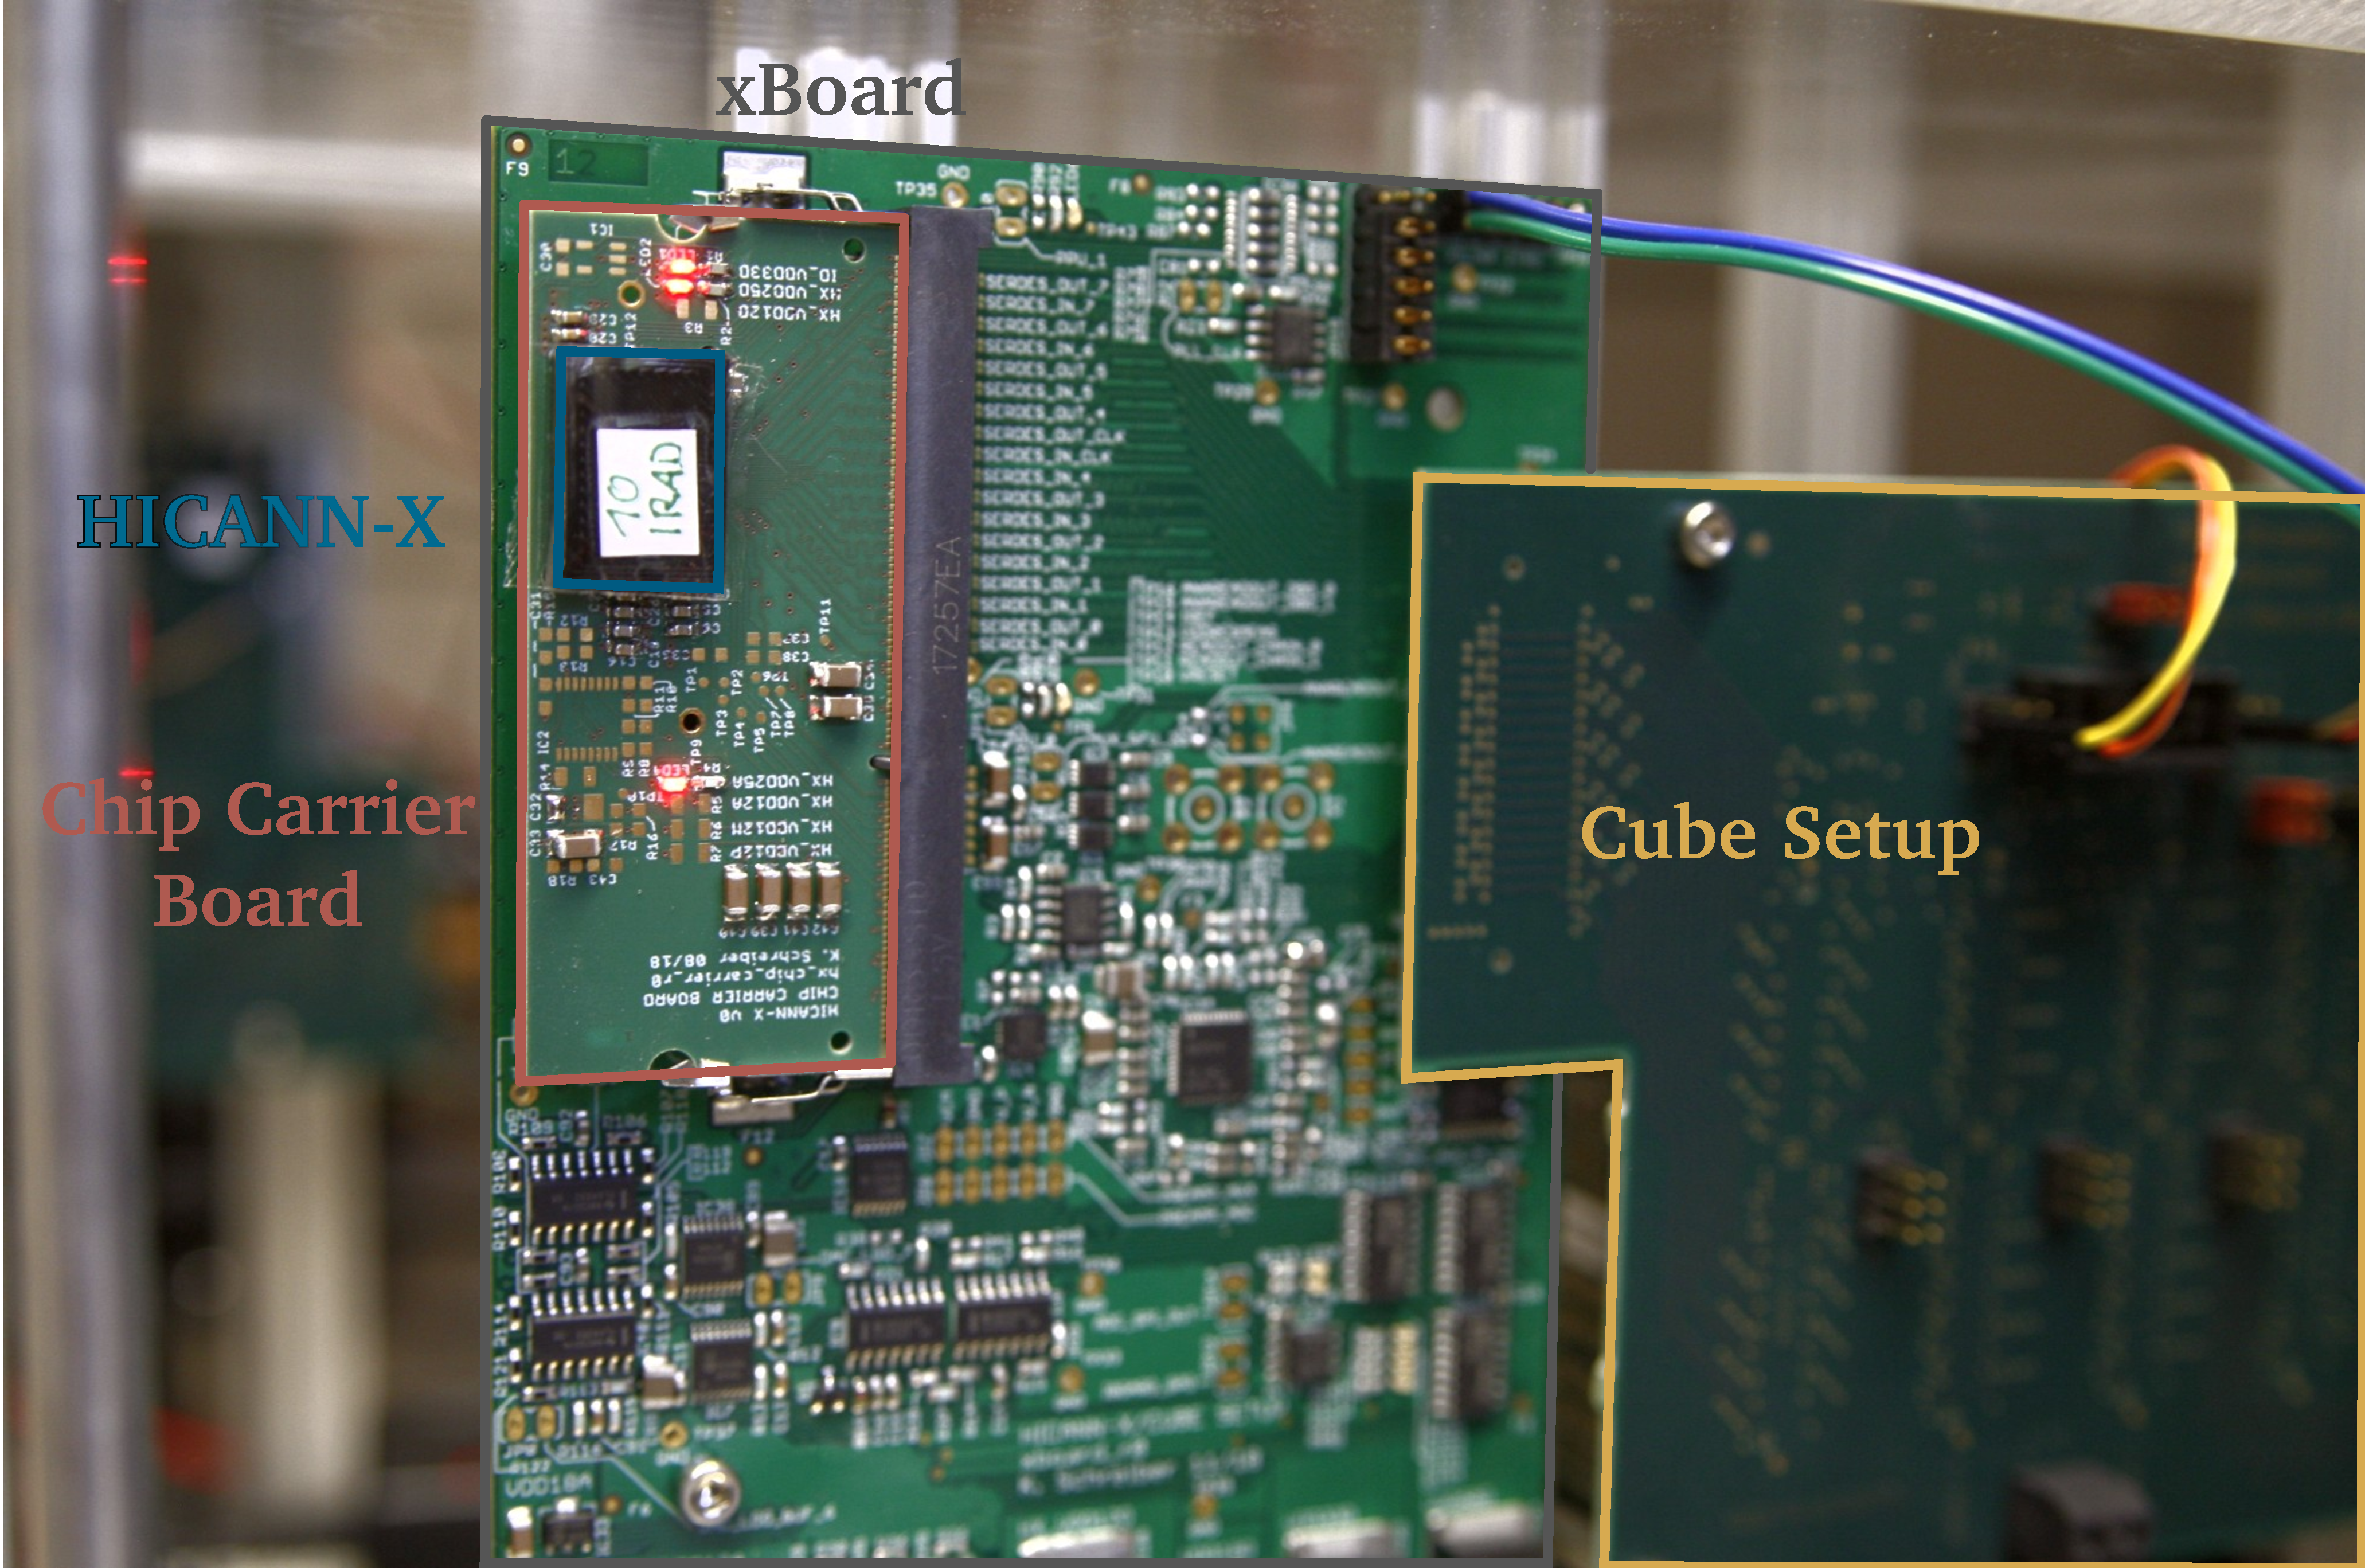
\includegraphics[width=0.98\textwidth]{figures/hxsetup_img_close_edited2.pdf}
		\label{cubesetup}
	\end{subfigure}	
	\begin{subfigure}{0.49\textwidth}
		\centering
		\caption{}
		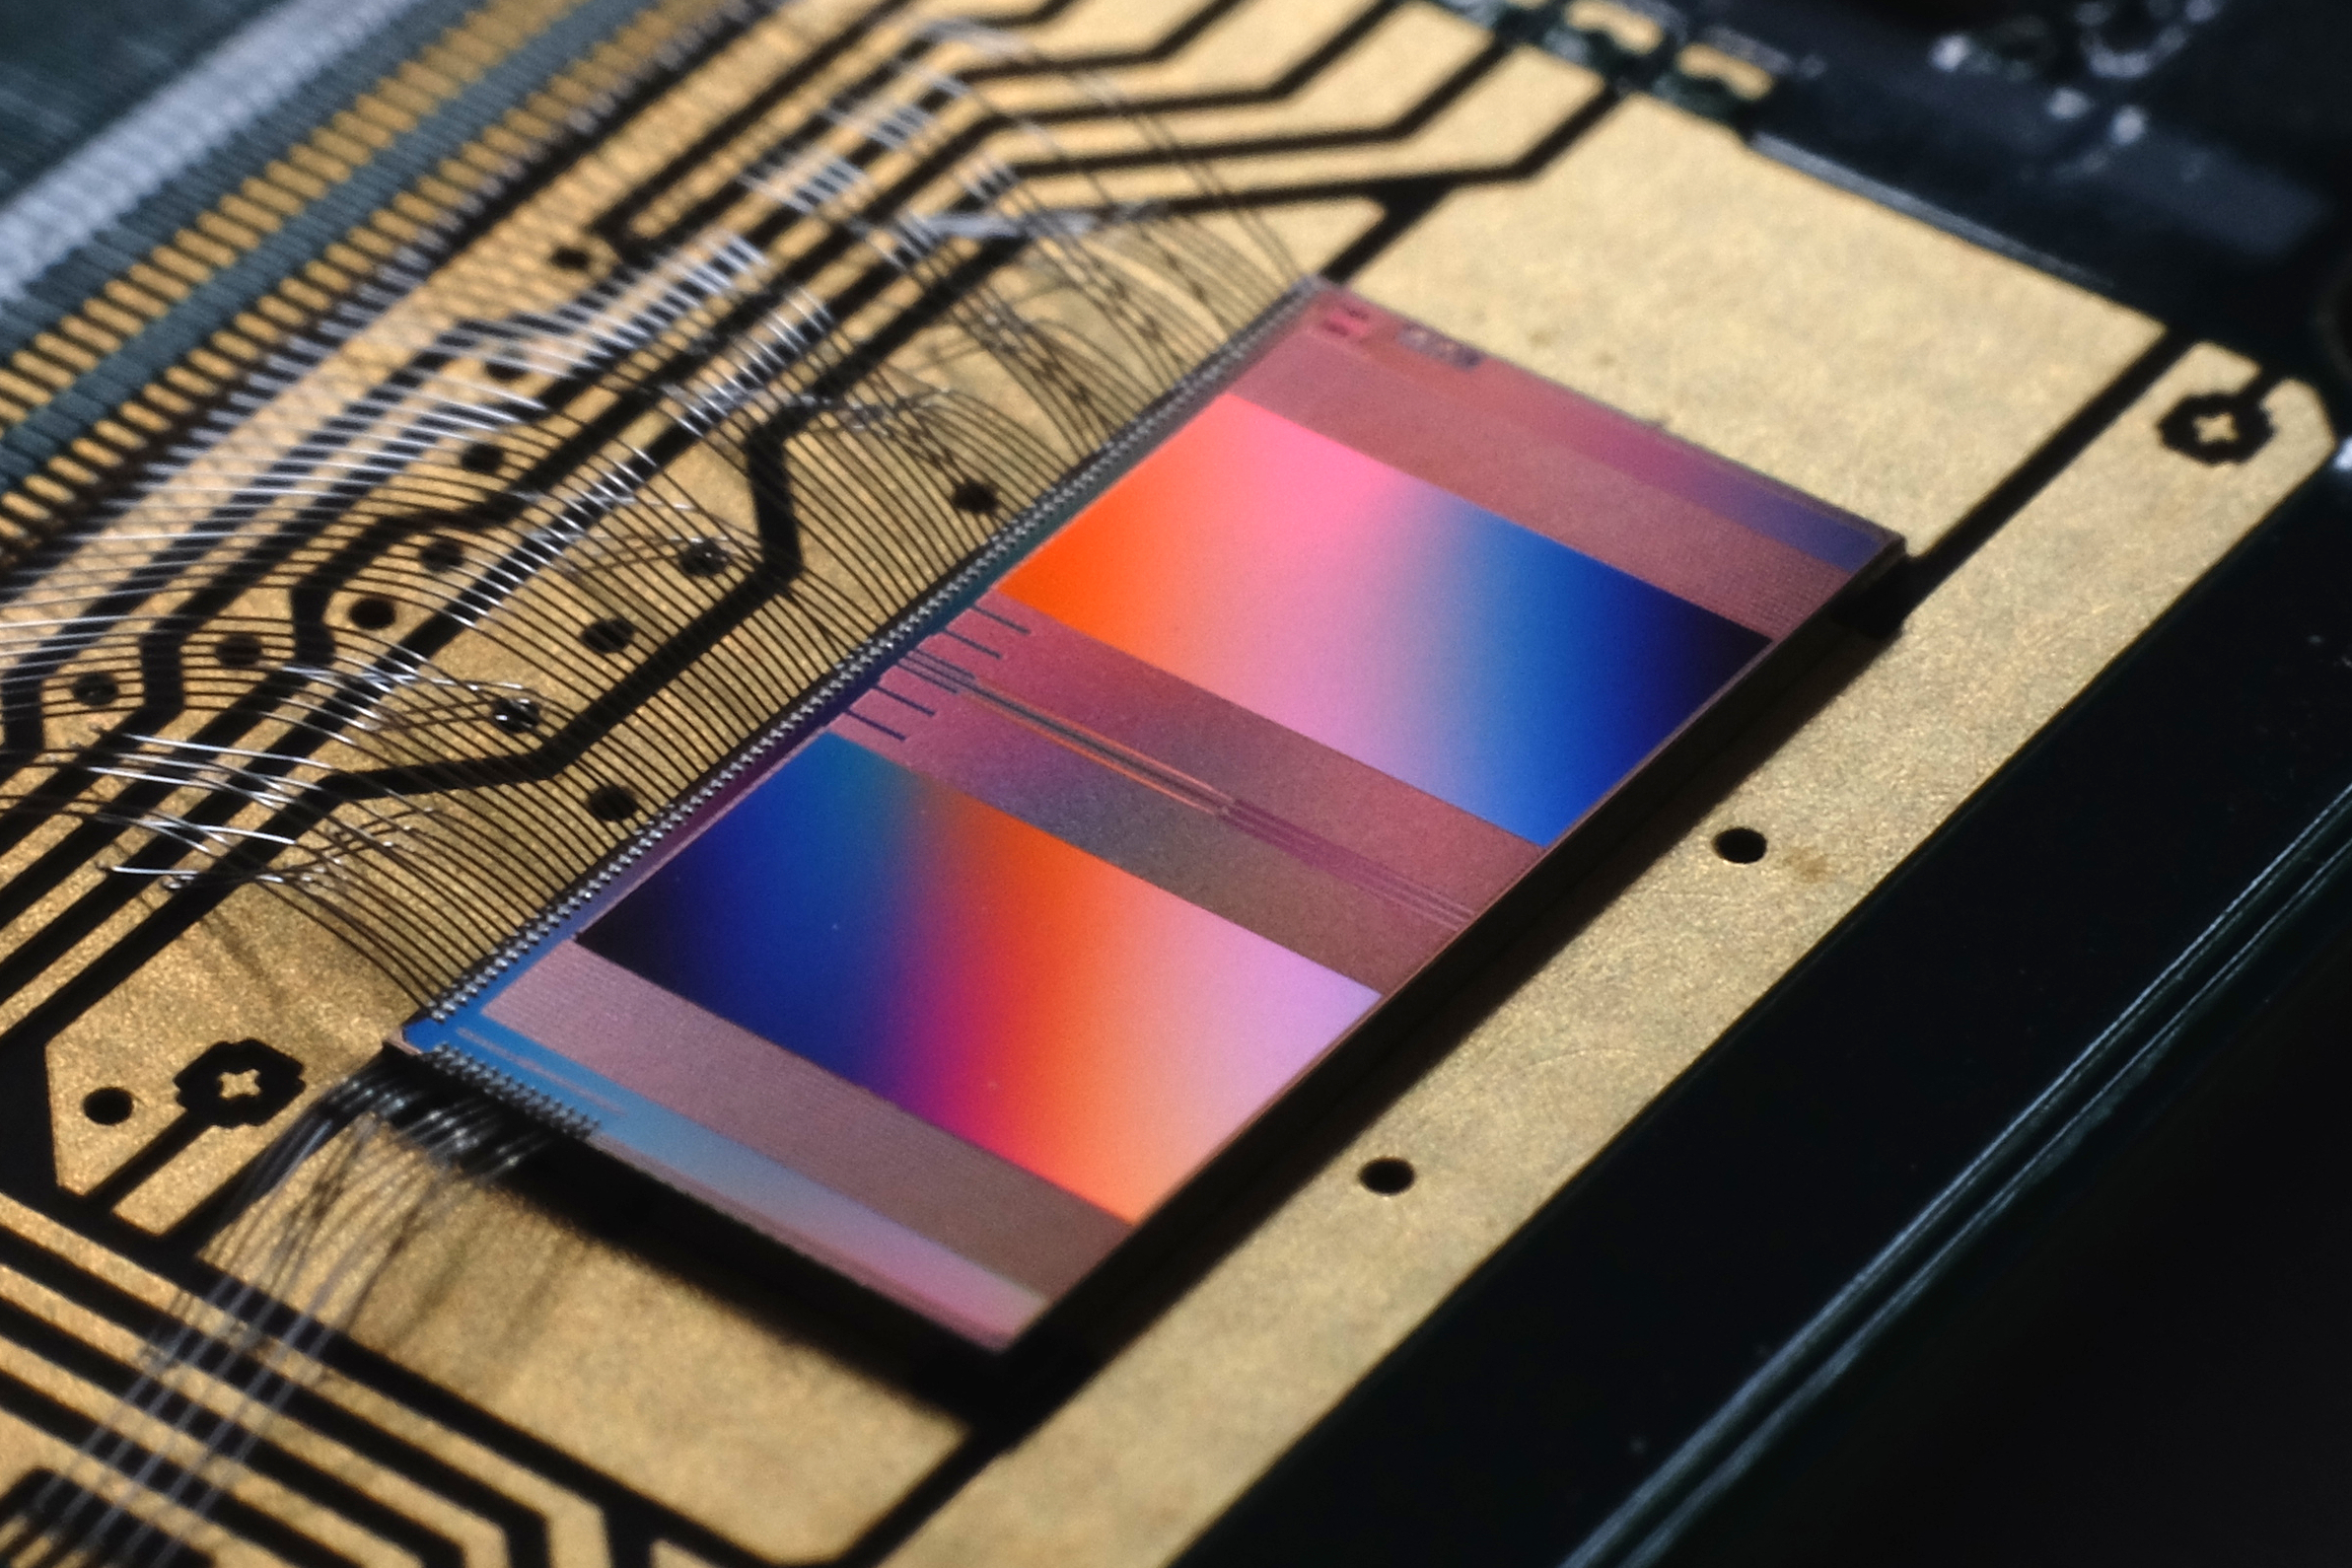
\includegraphics[width=.98\textwidth]{figures/HXcloseup.JPG}
		\label{hxcloseup}
	\end{subfigure}
	\centering
	\caption[The \acrshort{hx} setup.]{The \acrshort{hx} setup. \textbf{(\subref{cubesetup})} The chip (\textit{blue}) is mounted on a carrier board and protected by a cover. The carrier board (\textit{red}) is then mounted on the xBoard (\textit{gray}) which is connected to the \acrshort{fpga} over the cube setup (\textit{yellow}). \textbf{(\subref{hxcloseup})} Close-up of the newest \gls{bss2} single chip. The analog core of the neuromorphic chip is bonded before a protective cover is placed over it. Picture taken by M{\"u}ller, 2020.} 
	\label{hxsetup}
\end{figure}

In the context of this thesis, the presented learning strategies from \cref{neuralcoding} are implemented on an analog neuromorphic platform called \glsfirst{bss2}. This mixed-signal accelerated emulation for \glspl{snn} is based in Heidelberg and is the result of a long term cooperation with the EU, namely the Human Brain Project (HBP).
%
The \gls{bss2} platform is designed to perform various plasticity algorithms on-chip. The core of the platform is based upon a complete redesign of its predecessor the \gls{hicann}. By reducing the CMOS manufacturing process from \SI{180}{\nano \m} to \SI{65}{\nano \m} several new features could be included on the new core. One of the main renewals is a general purpose unit which can be used for any on-chip computation and a specialized vector unit that efficiently provides parallel access to observables from the analog core. The features have been implemented step by step on various prototype versions. The following paragraphs will focus on the specifications of the prototypes used for the experimental implementations of the discussed deep learning methods (c.f. \cref{bss2prototypes}).

On the \gls{dls} the newly designed \gls{lif} neuron model was tested as well as the on-chip computational units. The latter are also summarized as the \gls{ppu}. The \gls{dls} was manufactured at a reduced size of $32$ neurons and $32 \times 32$ synapses to avoid unnecessary costs. The \gls{hx} is the first full-size prototype of the \gls{bss2} platform with 512 \gls{adex} neuron circuits and 256 possible synaptic connections per neuron. In addition to the \gls{ppu}, the chip features on-chip event routing and HAGEN extension, an early realization of a neuromorphic system which basically implements an on-chip analog matrix multiplication (\citealp{schemmel2020accelerated}). Another renewal are dedicated noise generators, which come in handy when working with sigmoid activation functions and rate coding (c.f. \cref{ratecoding}).

\begin{table}[t!]\centering\ra{1.3}
	\begin{tabular}{@{}rccccc@{}}\toprule
		& 					& Neuron Model	& Neurons 	& Synapses 	& DLS	\\ \midrule
		& \acrshort{dls}	& \gls{lif}		& 32 		& $32 \times 32$	& \gls{ppu}\\
		& \acrshort{hx}		& \gls{adex}	& 512	 	& $512 \times 256$	& \gls{ppu}, Hagen\\
		\bottomrule
	\end{tabular}
	\caption[Overview of relevant \gls{bss2} prototypes.]{Overview of relevant \gls{bss2} prototypes. On \acrshort{dls} a rate-based \gls{snn} is successfully trained by a fully on-chip implementation and on \acrshort{hx} a temporal-based \gls{snn} is successfully trained with support from a host.}
	\label{bss2prototypes}
\end{table}

%The new features have been implemented step by step on various prototype versions. On the \gls{dls} the newly designed \gls{lif} neuron model was tested in combination with a in a reduced size of only $32$ neurons and a corresponding $32 \times 32$ synapse array allows all to all connectivity. The \gls{dls} and \gls{hx} chip. The \gls{hx} is the first full-size prototype of the \gls{bss2} platform with 512 \gls{adex} neuron circuits and 256 possible synaptic connections per neuron is especially designed to investigate various on-chip plasticity algorithms. Therefore it features two \glspl{ppu}, on-chip event routing and the HAGEN extension. The latter is an early realization of a neuromorphic system which basically implements analog matrix multiplication on-chip (\citealp{schemmel2020accelerated}).

%The new features have been tested step by step on smaller prototype systems, e.g. on the \gls{dls} the newly designed \gls{lif} neuron was tested. To avoid unnecessary costs, the size was reduced to $32$ neurons and a corresponding $32 \times 32$ synapse array allows all to all connectivity. Besides the Hagen extension and the \gls{adex} neuron, the main features of the \gls{bss2} platform, such as the \gls{ppu}, are already available on the prototyped versions.

%The experiments conducted within this thesis are done either on the \gls{hx} or the \gls{dls}. In the following section the individual parts of the chip are discussed.
%The manufacturing has been outsourced to the Taiwan Semiconductor Manufacturing Company (TSMC) using a standardized $65 \si{nm}$ low-power and low-leakage CMOS technology.

\subsection{Architecture of \gls{bss2}}

\begin{figure}
	\begin{subfigure}[c]{0.5\textwidth}
		\centering
		\caption{}
		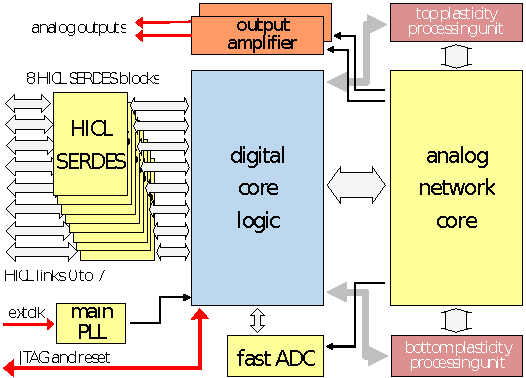
\includegraphics[width=0.9\textwidth]{figures/bss2architecture_wtext.pdf}
		\label{hxstructure}
	\end{subfigure}	
	\begin{subfigure}[c]{0.5\textwidth}
		\centering
		\caption{}
		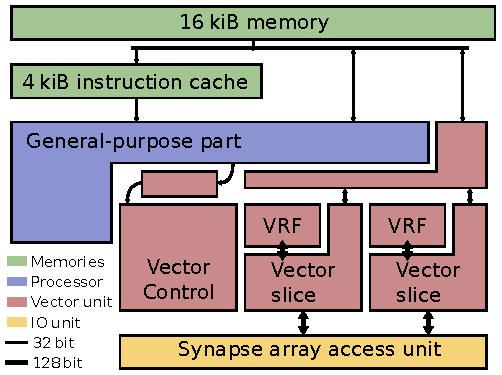
\includegraphics[width=0.9\textwidth]{figures/ppu_overview.pdf}
		\label{hxppu}
	\end{subfigure}
	\caption[Overview of the \gls{bss2} architecture.]{Overview of the \gls{bss2} architecture. \textbf{(\subref{hxstructure})} The neuromorphic platform is divided into a digital and analog core which is connected to an external host via an FPGA. Two plasticity processing units provide computational power for on-chip training.  Figure taken from \citealp{schemmel2017internal} \textbf{(\subref{hxppu})} The plasticity processing units are divided into a general purpose part which is based on a 32-bit architecture and a vector unit. The latter enables efficient parallel data processing of analog parameters and observables. Figure taken from \cite{friedmann2016hybridlearning}}
\end{figure}

The design of both prototypes can be divided into an \emph{analogue} and a \emph{digital} core (c.f. figure \ref{hxstructure}). The external communication is established by an \gls{fpga} accessing eight serial Low Voltage Differential Signaling (LVDS) links. The interface not only manages read and write instructions but handles any spike-event data in both directions.

Depending on the chip version, the analogue core contains the physical implementation of either a \gls{lif} or an \gls{adex} neuron model (\citealp{aamir2018dls2neuron} and \citealp{aamir2018mixed}). The analog neuron model parameters can be tuned by setting respective bias currents with a \SI{10}{\bit} \gls{dac}. Each neuron can be controlled and adjusted individually (\citealp{hock13analogmemory}). 

The biological time constants of neurons and synapses are usually in the order of 1 to 100 milliseconds. The \textit{in-silico} implementation of the neuron models cause a temporal speed-up compared to their \textit{in-vivo} counterpart, leading to chip-time constants of a few microseconds. This acceleration is possible due to the supra-threshold dynamics of CMOS transistors. 

\begin{figure}
	\centering
	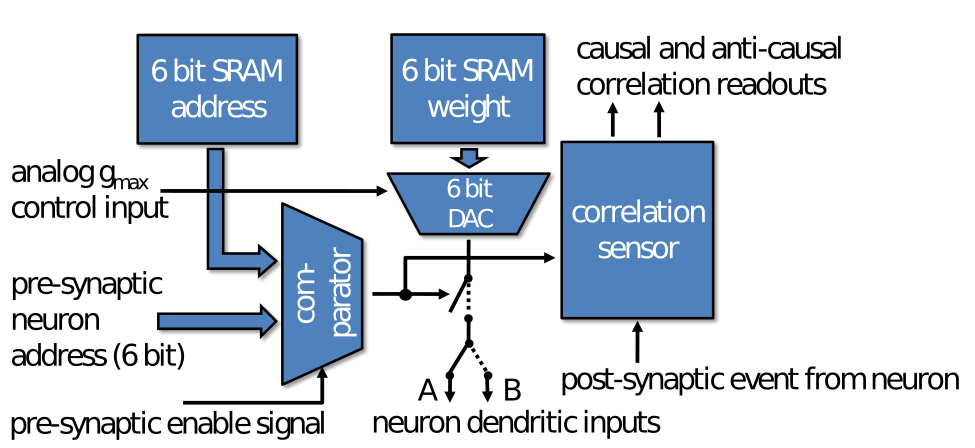
\includegraphics[width=0.8\textwidth]{figures/synapse.png}
	\caption[Synapse circuit overview on \gls{dls}]{Synapse circuit overview on \gls{dls}. Synapse drivers inject the presynaptic activity row-wise as either inhibitory or excitatory spikes. The 6-bit addresses of the presynaptic neuron is compared at each synapse with a local \SI{6}{\bit} address. If the addresses match, the spike is relayed to the corresponding neuron at the bottom of the synapse grid. The synaptic strength can be configured by a \SI{6}{\bit} weight. The two correlation sensors (causal and anti-causal) record \gls{stdp} traces. Figure from \cite{friedmann2016hybridlearning}.}
	\label{synapseschematics}
\end{figure}

On the full-size chip, the neurons are connected by a grid of $512 \times 256$ synapses ($32 \times 32$ on the smaller one). The activity of presynaptic neurons is injected row-wise by dedicated synapse drivers as either excitatory or inhibitory spikes. Each synapse has access to a \SI{6}{\bit} decoder address and compares it to a 6-bit label of the incoming spikes (see \cref{synapseschematics}). If they match, the spike is relayed to the corresponding neuron at the bottom of the synapse grid. The efficacy is thereby configured by a \SI{6}{\bit} weight.

The analog core features several observables which are relevant for the implementation of plasticity rules. The firing rate of a neuron for instance is recorded by a \SI{10}{\bit} spike counter on the \gls{dls}. The counter has been replaced by a smaller \SI{8}{\bit} version on the full-size chip to save some space. In addition, every synapse features two correlation sensors (causal and anti-causal) which are designed to record \gls{stdp} traces. Other relevant observables are the traces of the synaptic input current or the membrane potential. The latter is key for the implementation of temporal-based plasticity rules such as SuperSpike.

When training a highly accelerated analog system such as \gls{bss2} platform, a fast computation of any plasticity rule is indispensable. A \gls{cadc} provides row-wise parallel access to the \gls{stdp} traces with a total of $2 \times 32$ respectively $2 \times 512$ \gls{cadc} channels (one channel per correlation sensor per synapse row). The on-chip vector unit then guarantees an efficient access to the \gls{cadc} readout by the use of \gls{simd} operations. On the newer \gls{hx}, the \gls{cadc} routing possibilities have been extended such that the membrane potential can be accessed as well. Before this renewal the membrane potential was recorded by an \gls{madc} which accesses only one neuron at a time. With the lack of parallelization a fast in-experiment use cannot be realized and is therefor feasible for training purposes. This limitation is compensated by a better accuracy and resolution making the \gls{madc} a useful debugging and observation tool.

Apart from dedicated spike counters, the digital neuron back end registers any spiking event and transfers them to the digital core logic, where the events are merged with any activity coming from the noise spike generators or \glspl{ppu} as well as from an external source. The events are then rerouted back into the synapse grid accordingly, enabling recurrent connections and multilayer network structures.

These observation features for the analog neuronal dynamics are then combined by the general purpose unit with which complex plasticity rules can be implemented on-chip (see \cref{hxppu}). The \gls{hx} features even a second \glspl{ppu} to provide enough computational power for the increased chip size. The software capabilities of the general purpose unit for the new chip are under continuous development. For instance a fast access to an external memory will be released in near future. The current hardware and software constraints of both prototypes will be discussed in a final chapter, after the experimental implementations have been presented (\cref{circles} and \cref{superspike}).

%On the newer \gls{hx}, the \gls{cadc} is equipped with more routing possibilities, with which the membrane potential can be accessed as well. This feature  Unlike the \gls{cadc} the \gls{madc} provides only access to one observable at a time. This limitation is compensated with a better accuracy, making it a useful debugging and observation tool, that can be accessed from the digital core of the chip. By the use of the \gls{madc} the membrane potential can also be recorded on the \gls{dls}. However, with the lack of parallelization an in-experiment use is not feasible.
%When training a highly accelerated analog system, such as \gls{bss2}, a fast computation of any plasticity rule is indispensable. To provide sufficient computational power, the chip is equipped with two \glspl{ppu}, each containing a general-purpose unit that is extended with a special function unit implementing \gls{simd} operations. The special function unit has vector-wise access to the synapse array as well as to the results of the \gls{cadc} and will be further referred to as \emph{vector unit}.
%The communication with an external host is streamed out to the controlling Field Programmable Gate Array (FPGA). The existing FPGA solution developed for \gls{bss1} was simply transfered to \gls{bss2}.
%The link between chip and external host is established via an \gls{fpga} accessing eight serial Low Voltage Differential Signaling (LVDS) links. This interface handles read/write instructions and manages spike event data in both directions. %The FPGA grants access for the PPU to greater memory storages than the one provided on-chip. Access to large training datasets is vital for most learning tasks.